\pagebreak

\chapter{Κεφάλαιο 1 ---
Εισαγωγή}\label{ux3baux3b5ux3c6ux3acux3bbux3b1ux3b9ux3bf-1-ux3b5ux3b9ux3c3ux3b1ux3b3ux3c9ux3b3ux3ae}

\section{1.1 Πλαίσιο της
εργασίας}\label{ux3c0ux3bbux3b1ux3afux3c3ux3b9ux3bf-ux3c4ux3b7ux3c2-ux3b5ux3c1ux3b3ux3b1ux3c3ux3afux3b1ux3c2}

Η A.P. Møller-Mærsk A/S είναι ένας από τους μεγαλύτερους ομίλους
ολοκληρωμένης εφοδιαστικής αλυσίδας παγκοσμίως. Ιδρυθείσα το 1904, η
εταιρεία δραστηριοποιείται σε περισσότερες από 130 χώρες, απασχολεί πάνω
από 100.000 εργαζομένους και λειτουργεί στόλο άνω των 700 πλοίων
κοντέινερ --- τοποθετώντας την μεταξύ των δύο ή τριών μεγαλύτερων
\emph{container carriers} παγκοσμίως. Πέραν της θαλάσσιας μεταφοράς, ο
όμιλος επεκτείνεται σε Logistics \& Services, Terminals και Towage,
υλοποιώντας τη στρατηγική μετατόπιση από αποκλειστικό \emph{shipping
company} σε \emph{integrated logistics provider}. Η κλίμακα αυτή
συνεπάγεται τεράστιο ενεργειακό αποτύπωμα και, συνακόλουθα, τεράστια
ευθύνη στη διαχείριση των εκπομπών αερίων θερμοκηπίου (\emph{greenhouse
gases} --- GHG).

Η θαλάσσια μεταφορά αποτελεί τη ραχοκοκαλιά του παγκόσμιου εμπορίου,
μεταφέροντας περίπου το 80-90\% των εμπορευμάτων που κινούνται διεθνώς.
Παρά την αποτελεσματικότητά της ανά τόνο-χιλιόμετρο συγκριτικά με άλλες
μορφές μεταφοράς, η ναυτιλία συνεισφέρει σημαντικά στις παγκόσμιες
εκπομπές CO₂. Σύμφωνα με την Τέταρτη Μελέτη Εκπομπών GHG του Διεθνούς
Ναυτιλιακού Οργανισμού (IMO 4th GHG Study, 2020), η διεθνής ναυτιλία
ευθύνεται για περίπου \textbf{3\% των παγκόσμιων εκπομπών CO₂} ετησίως.
Η απανθρακοποίηση του κλάδου αντιμετωπίζει ιδιαίτερες δυσκολίες: τα
πλοία έχουν ωφέλιμη ζωή 25-30 ετών, απαιτούν εξαιρετικά υψηλή ενεργειακή
πυκνότητα που καθιστά την αντικατάσταση των συμβατικών υδρογονανθράκων
από εναλλακτικά καύσιμα τεχνολογικά απαιτητική, και δραστηριοποιούνται
σε διεθνή ύδατα εκτός ενιαίου εθνικού ρυθμιστικού πλαισίου. Σε αυτό το
πλαίσιο, η Maersk έχει θέσει στόχο \textbf{καθαρών μηδενικών εκπομπών
έως το 2040} --- δέκα χρόνια νωρίτερα από τον αντίστοιχο στόχο της IMO
για το 2050 --- με ενδιάμεσο ορόσημο χρήσης τουλάχιστον \textbf{30\%
βιώσιμης ενέργειας έως το 2030}.

Παράλληλα, το ρυθμιστικό περιβάλλον έχει εντατικοποιηθεί σημαντικά τα
τελευταία χρόνια. Η \textbf{Οδηγία CSRD} (\emph{Corporate Sustainability
Reporting Directive}) επιβάλλει εκτεταμένες υποχρεώσεις αναφοράς
βιωσιμότητας για μεγάλες ευρωπαϊκές οντότητες. Το \textbf{EU ETS
Maritime} --- η επέκταση του Ευρωπαϊκού Συστήματος Εμπορίας Εκπομπών στη
ναυτιλία --- τέθηκε σε ισχύ από \textbf{1/1/2024}, με σταδιακή αύξηση
των αποδοτέων εκπομπών (40\% το 2024, 70\% το 2025, 100\% από το 2026).
Η κανονιστική πράξη \textbf{FuelEU Maritime}, που εφαρμόζεται από
\textbf{1/1/2025}, θεσπίζει ποιοτικούς στόχους για την ένταση GHG των
καυσίμων. Τέλος, η αναθεωρημένη στρατηγική GHG της IMO (MEPC 80, 2023)
εντατικοποιεί τους στόχους μείωσης εκπομπών έως το 2030 και 2050. Η
συνδυαστική πίεση αυτών των ρυθμίσεων απαιτεί από εταιρείες της κλίμακας
της Maersk επίπεδα ακρίβειας, ιχνηλασιμότητας και αξιοπιστίας στη
μέτρηση εκπομπών που δεν μπορούν να επιτευχθούν με χειρωνακτικές
διαδικασίες. Τα λεπτομερή στοιχεία του ρυθμιστικού πλαισίου αναλύονται
στο Κεφ. 2.

\section{1.2 Στόχος της
εργασίας}\label{ux3c3ux3c4ux3ccux3c7ux3bfux3c2-ux3c4ux3b7ux3c2-ux3b5ux3c1ux3b3ux3b1ux3c3ux3afux3b1ux3c2}

Η παρούσα διπλωματική εργασία παρουσιάζει τον \textbf{Πάγκο Εργασίας
Εκπομπών} (\emph{Emissions Workbench}) --- την κεντρική πλατφόρμα
λογισμικού που σχεδίασε και υλοποίησε η ομάδα \emph{Energy Transition
(ET) Platform} της Maersk κατά το διάστημα Μαρτίου 2023 εώς σήμερα.
Στόχος της εργασίας είναι η τεκμηριωμένη παρουσίαση της λύσης σε
τέσσερις αλληλοσυμπληρούμενες διαστάσεις: τις λειτουργικές ανάγκες και
το επιχειρησιακό πλαίσιο που ώθησαν στη δημιουργία της, τις τεχνολογικές
αποφάσεις και αρχιτεκτονικές επιλογές που διέπουν την υλοποίησή της, τη
μεθοδολογία ανάπτυξης της ομάδας, και τα επιχειρησιακά αποτελέσματα που
επιτεύχθηκαν.

Αναλύεται η αρχιτεκτονική ενός συστήματος παραγωγικής κλίμακας που
συνδυάζει \emph{event-driven} επεξεργασία δεδομένων, \emph{event
sourcing} για λογιστική πράσινου καυσίμου, πραγματικού χρόνου
(\emph{real-time}) web διεπαφές και ολοκλήρωση με εξωτερικά συστήματα
τηλεμετρίας, αγορών καυσίμου και πιστοποίησης βιωσιμότητας. Εξετάζονται
επίσης οι εργασιακές μέθοδοι \emph{Extreme Programming} στο πλαίσιο μιας
κατανεμημένης ομάδας 28 μελών, και το πώς αυτές επέτρεψαν έναν κύκλο
ανάπτυξης έξι μηνών έως παραγωγική λειτουργία.

Η εργασία δεν καλύπτει εμπορικά ή συμβασιακά ζητήματα της Maersk,
λεπτομέρειες τιμολόγησης προς πελάτες, ή αισθητά προσωπικά δεδομένα
χρηστών. Επίσης δεν αποτελεί αξιολόγηση εναλλακτικών λύσεων του αγοράς
ούτε συγκριτική μελέτη τεχνολογιών εκτός του πλαισίου της συγκεκριμένης
υλοποίησης.

\section{1.3 Συνεισφορές της
εργασίας}\label{ux3c3ux3c5ux3bdux3b5ux3b9ux3c3ux3c6ux3bfux3c1ux3adux3c2-ux3c4ux3b7ux3c2-ux3b5ux3c1ux3b3ux3b1ux3c3ux3afux3b1ux3c2}

Η συμβολή της παρούσας εργασίας εντοπίζεται σε έξι βασικούς άξονες:

\begin{itemize}
\item
  \textbf{Τεκμηριωμένη παρουσίαση των τεσσάρων πυλώνων του ET Platform.}
  Αποτυπώνεται η πλήρης αρχιτεκτονική των πυλώνων Ocean Emissions, ECO
  Product Delivery, Bunker Optimization και Net Zero 2040 --- η
  εσωτερική αποστολή τους, η τεχνική τους υλοποίηση και η αλληλεπίδρασή
  τους.
\item
  \textbf{Αρχιτεκτονική \emph{event-driven} με BEAM σε εμπορικό
  περιβάλλον παραγωγής.} Η εργασία τεκμηριώνει πώς η πλατφόρμα
  BEAM/Elixir και οι σχετικές τεχνολογίες (Phoenix LiveView, Commanded,
  Oban, Kafka) εφαρμόζονται σε ένα σύστημα υψηλής διαθεσιμότητας με
  \textasciitilde32 αναπτύξεις σε παραγωγή ημερησίως και 720+ migrations
  χωρίς διακοπή υπηρεσίας.
\item
  \textbf{Σύζευξη θεωρητικού πλαισίου με τεχνική υλοποίηση.} Τα πρότυπα
  λογιστικής εκπομπών GHG Protocol, ISCC, GLEC και οι κατηγορίες Scope
  1/2/3 δεν παρουσιάζονται μόνο θεωρητικά, αλλά συνδέονται άμεσα με τα
  αντίστοιχα σχεδιαστικά πρότυπα (\emph{trade factors}, \emph{mass
  balance}, \emph{book-and-claim}) που υλοποιήθηκαν στον κώδικα.
\item
  \textbf{Εμπειρία εφαρμογής πρακτικών XP σε \emph{production team} της
  Maersk.} Η εργασία προσφέρει εμπειρική τεκμηρίωση για το πώς
  \emph{pair programming}, \emph{test-driven development},
  \emph{continuous integration} και \emph{vertical ownership}
  λειτούργησαν στην πράξη.
\item
  \textbf{Επιχειρησιακά αποτελέσματα σε μετρήσιμο βάθος.} Η εργασία
  συνδέει τεχνικές επιλογές με επιχειρησιακά αποτελέσματα: 1.300+
  ενεργοί χρήστες, ECO Delivery αξίας 98.000 FFE / \$31 εκατομμυρίων USD
  για το 2024, αντιμετώπιση εσωτερικού ελέγχου GIA 2023, και αυτόματη
  παραγωγή πιστοποιητικών για ECOv1 και ECOv2.
\end{itemize}

\section{1.4 Δομή του
κειμένου}\label{ux3b4ux3bfux3bcux3ae-ux3c4ux3bfux3c5-ux3baux3b5ux3b9ux3bcux3adux3bdux3bfux3c5}

Η εργασία οργανώνεται σε δώδεκα κεφάλαια, τα οποία ακολουθούν μια λογική
πρόοδο από το ευρύτερο πλαίσιο στην τεχνική υλοποίηση και τα
αποτελέσματα.

\textbf{Κεφάλαιο 2 --- Πλαίσιο και πρόβλημα} αναπτύσσει εκτενώς τον
επιχειρησιακό και ρυθμιστικό χώρο μέσα στον οποίο αναπτύχθηκε η
πλατφόρμα: το προφίλ της Maersk, η συνεισφορά της ναυτιλίας στις
παγκόσμιες εκπομπές, ο στόχος Net Zero 2040, οι ρυθμιστικές υποχρεώσεις
(CSRD, EU ETS, FuelEU Maritime), η χειρωνακτική διαδικασία που προηγείτο
και ο εσωτερικός έλεγχος GIA 2023 που ανέδειξε τα κενά της.

\textbf{Κεφάλαιο 3 --- Θεωρητικό υπόβαθρο} παρουσιάζει το κανονιστικό
και επιστημονικό πλαίσιο λογιστικής αερίων θερμοκηπίου: το GHG Protocol,
τις κατηγορίες εκπομπών Scope 1/2/3, τις μεθοδολογίες μέτρησης TTW και
WTW, τη λογική \emph{mass balance} και \emph{book-and-claim}, και τα
πρότυπα ISCC, GLEC που διέπουν την πιστοποίηση βιωσιμότητας.

\textbf{Κεφάλαιο 4 --- Ο Πάγκος Εργασίας Εκπομπών: Επισκόπηση} εισάγει
την αποστολή και τη δομή της ομάδας ET Platform, παρουσιάζει τους
τέσσερις πυλώνες σε επίπεδο αποστολής, και προσφέρει μια πρώτη
επισκόπηση της διεπαφής χρήστη και των επιτευγμάτων της πλατφόρμας.

\textbf{Κεφάλαιο 5 --- Πυλώνας Α: Ocean Emissions και STAR Connect}
αναλύει τον πρώτο πυλώνα: την αυτοματοποιημένη συλλογή τηλεμετρίας
καυσίμων από τον στόλο μέσω του STAR Connect, τον υπολογισμό εκπομπών
ανά κίνηση εμπορευματοκιβωτίου βάσει \emph{trade factors}, την
ενσωμάτωση EU ETS και τον υπολογισμό \emph{baseline} εκπομπών πελατών.

\textbf{Κεφάλαιο 6 --- Πυλώνας Β: ECO Product Delivery και
πιστοποιητικά} εξετάζει τον εμπορικό πυλώνα της πλατφόρμας: τις δύο
μεθοδολογίες ECOv1 και ECOv2, τη λογιστική πράσινου καυσίμου μέσω του
\emph{Energy Bank}, την αδιάσπαστη αλυσίδα ιχνηλασιμότητας ISCC/POS και
την αυτόματη έκδοση πιστοποιητικών.

\textbf{Κεφάλαιο 7 --- Πυλώνας Γ: Bunker Optimization} περιγράφει το
σύστημα βελτιστοποίησης ανεφοδιασμού καυσίμου (BOPS και BoW), τον C++
solver που ενσωματώνεται μέσω Erlang Ports, και τη σύνδεση της
βελτιστοποίησης κόστους καυσίμου με την ευρύτερη στρατηγική πράσινης
μετάβασης.

\textbf{Κεφάλαιο 8 --- Τεχνολογίες} παρουσιάζει αναλυτικά τις
τεχνολογίες της πλατφόρμας: BEAM/Elixir, Phoenix/LiveView,
PostgreSQL/Ecto, Apache Kafka, Dremio, Microsoft Azure/Kubernetes,
Terraform, Nix, Oban, Commanded/EventStore και το σύνολο του
\emph{observability stack}.

\textbf{Κεφάλαιο 9 --- Αρχιτεκτονική του συστήματος} αναλύει την
οργάνωση του monorepo \texttt{:nrg}, την εφαρμογή της \emph{Clean
Architecture}, τα components και τα όριά τους, το pipeline εισαγωγής
δεδομένων, το web layer, την αυθεντικοποίηση και εξουσιοδότηση, τη
λογική \emph{event sourcing} για την Energy Bank και την στρατηγική
deployment.

\textbf{Κεφάλαιο 10 --- Εργασιακές μέθοδοι} εξετάζει τις πρακτικές
\emph{Extreme Programming} που υιοθέτησε η ομάδα: \emph{pair
programming}, \emph{TDD}, \emph{continuous integration/delivery},
\emph{vertical ownership}, \emph{feedback loops}, \emph{onboarding} και
συνεργασίας σε κατανεμημένο περιβάλλον.

\textbf{Κεφάλαιο 11 --- Συμπεράσματα} συνοψίζει τα κύρια ευρήματα,
αξιολογεί τα επιτεύγματα σε σχέση με τους αρχικούς στόχους και
αναδεικνύει τα μαθήματα από την υλοποίηση που έχουν μεταφερσιμότητα
πέραν του συγκεκριμένου έργου.

\textbf{Κεφάλαιο 12 --- Μελλοντική εργασία} σκιαγραφεί τις επεκτάσεις
που ήδη σχεδιάζονται ή συζητιούνται: κάλυψη εκπομπών Scope 2 από γραφεία
και τερματικά, επέκταση αναφοράς SBTi, προβλεπτικά analytics και
ενσωμάτωση Bunker Optimization με την Energy Bank.

\pagebreak

\chapter{Κεφάλαιο 2 --- Πλαίσιο και
πρόβλημα}\label{ux3baux3b5ux3c6ux3acux3bbux3b1ux3b9ux3bf-2-ux3c0ux3bbux3b1ux3afux3c3ux3b9ux3bf-ux3baux3b1ux3b9-ux3c0ux3c1ux3ccux3b2ux3bbux3b7ux3bcux3b1}

Το παρόν κεφάλαιο διαγράφει το ευρύτερο πλαίσιο μέσα στο οποίο
αναπτύχθηκε ο Πάγκος Εργασίας Εκπομπών (\emph{Emissions Workbench}).
Αρχικά παρουσιάζεται η ίδια η Maersk ως επιχείρηση και ο κλάδος
θαλάσσιων μεταφορών, στη συνέχεια αναλύεται το ρυθμιστικό και
επιχειρησιακό πρόβλημα που έκανε αναγκαία την ανάπτυξη μιας
ολοκληρωμένης λύσης, και τέλος εξετάζονται οι συγκεκριμένοι καταλύτες
--- χρήστες, χειρωνακτικές διαδικασίες, εσωτερικός έλεγχος --- που
ώθησαν στη δημιουργία του συστήματος.

\section{2.1 Η Maersk και ο τομέας της θαλάσσιας
μεταφοράς}\label{ux3b7-maersk-ux3baux3b1ux3b9-ux3bf-ux3c4ux3bfux3bcux3adux3b1ux3c2-ux3c4ux3b7ux3c2-ux3b8ux3b1ux3bbux3acux3c3ux3c3ux3b9ux3b1ux3c2-ux3bcux3b5ux3c4ux3b1ux3c6ux3bfux3c1ux3acux3c2}

Η A.P. Møller-Mærsk A/S είναι μια δανέζικη πολυεθνική εταιρεία με έδρα
στην Κοπεγχάγη, ιδρυθείσα το 1904 από τον Arnold Peter Møller και τον
πατέρα του Peter Mærsk Møller. Από μια μικρή ατμοπλοϊκή εταιρεία του
19ου αιώνα, η Maersk εξελίχθηκε σε έναν από τους μεγαλύτερους ομίλους
ολοκληρωμένης εφοδιαστικής αλυσίδας παγκοσμίως, με παρουσία σε
περισσότερες από 130 χώρες και πάνω από 100.000 εργαζομένους.

Ο όμιλος δραστηριοποιείται σε τέσσερις βασικούς τομείς: \textbf{Ocean}
(ναυτιλία κοντέινερ), \textbf{Logistics \& Services} (αποθήκευση,
διανομή, τελωνειακές υπηρεσίες), \textbf{Terminals} (εμπορικά λιμάνια
και τερματικοί σταθμοί) και \textbf{Towage} (ρυμουλκητικές εργασίες). Ο
τομέας Ocean αποτελεί τον κορμό των δραστηριοτήτων: το 2023-2024 ο
στόλος της Maersk αριθμούσε περί τα 700 πλοία κοντέινερ, με συνολική
μεταφορική ικανότητα που τοποθετεί την εταιρεία μεταξύ των δύο ή τριών
μεγαλύτερων container carriers παγκοσμίως, διακινώντας εκατομμύρια TEU
(\emph{Twenty-foot Equivalent Units}) ετησίως σε κύρια εμπορικά
δρομολόγια όλων των ωκεανών.

Τις τελευταίες δεκαετίες, η Maersk πραγματοποίησε μια στρατηγική
μετατόπιση από καθαρά \emph{container shipping company} σε
\emph{integrated logistics provider}. Η εξαγορά της Hamburg Süd (2017),
της Damco (ενσωμάτωση), της LF Logistics (2022) και πολλών άλλων
εταιρειών logistics σηματοδοτεί αυτή τη στρατηγική βούληση. Στόχος είναι
η παροχή end-to-end εφοδιαστικών λύσεων --- από το εργοστάσιο παραγωγής
έως την πόρτα του καταναλωτή --- κάτω από μία οροφή, μειώνοντας την
πολυπλοκότητα για τους πελάτες και αυξάνοντας την προστιθέμενη αξία
πέραν της απλής θαλάσσιας μεταφοράς.

Αυτή η επιχειρηματική εξέλιξη συνεπάγεται και αλλαγή του αποτυπώματος
CO₂ της εταιρείας: πέραν των εκπομπών από πλοία (Κατηγορία 1 στο GHG
Protocol, βλ. Κεφ. 3), προστίθενται εκπομπές από εγκαταστάσεις
αποθήκευσης, φορτηγά μεταφοράς τελευταίου μιλίου, αεροπορικές αποστολές
και αλυσίδες εφοδιασμού τρίτων (Κατηγορία 3). Συνεπώς η διαχείριση των
εκπομπών δεν αφορά μόνο τον στόλο, αλλά ολόκληρο το επιχειρηματικό
οικοσύστημα.

\section{2.2 Συνεισφορά της ναυτιλίας στις παγκόσμιες
εκπομπές}\label{ux3c3ux3c5ux3bdux3b5ux3b9ux3c3ux3c6ux3bfux3c1ux3ac-ux3c4ux3b7ux3c2-ux3bdux3b1ux3c5ux3c4ux3b9ux3bbux3afux3b1ux3c2-ux3c3ux3c4ux3b9ux3c2-ux3c0ux3b1ux3b3ux3baux3ccux3c3ux3bcux3b9ux3b5ux3c2-ux3b5ux3baux3c0ux3bfux3bcux3c0ux3adux3c2}

Η θαλάσσια μεταφορά αποτελεί τη ραχοκοκαλιά του παγκόσμιου εμπορίου:
περίπου το 80-90\% των εμπορευμάτων που κινούνται παγκοσμίως
μεταφέρονται δια θαλάσσης. Παρά την τεράστια αυτή αποτελεσματικότητα σε
σχέση με άλλες μορφές μεταφοράς ως προς εκπομπές ανά τόνο-χιλιόμετρο, η
ναυτιλία στο σύνολό της συνεισφέρει σημαντικά στις παγκόσμιες εκπομπές
αερίων θερμοκηπίου (\emph{greenhouse gases} --- GHG).

Σύμφωνα με την Τέταρτη Μελέτη Εκπομπών GHG του Διεθνούς Ναυτιλιακού
Οργανισμού (IMO 4th GHG Study, 2020), η διεθνής ναυτιλία ευθύνεται για
περίπου \textbf{2,89\% των παγκόσμιων εκπομπών CO₂} ετησίως, αριθμός που
αντιστοιχεί σε περίπου 1.056 εκατομμύρια τόνους CO₂ για το 2018. Αν
συμπεριληφθούν και άλλα αέρια θερμοκηπίου (μεθάνιο, υποξείδιο του
αζώτου), το ποσοστό ανέρχεται σε \textasciitilde2,5\% των συνολικών
ανθρωπογενών εκπομπών GHG. Αν συνυπολογίσει κανείς ότι η ναυτιλία
αναμένεται να αυξήσει τους όγκους της παράλληλα με την παγκόσμια
οικονομική ανάπτυξη, η IMO εκτιμά ότι χωρίς παρέμβαση οι εκπομπές θα
μπορούσαν να αυξηθούν κατά 50\% έως 250\% έως το 2050 σε σχέση με το
2008.

Τα κυρίαρχα καύσιμα ναυτιλίας παραμένουν τα βαριά καύσιμα
υδρογονανθράκων: \textbf{HFO} (\emph{Heavy Fuel Oil} --- βαρύ
πετρέλαιο), \textbf{VLSFO} (\emph{Very Low Sulfur Fuel Oil} ---
ναυτιλιακό πετρέλαιο πολύ χαμηλής περιεκτικότητας θείου, εισαχθέν μετά
τον κανονισμό IMO 2020 για τα θείωδη) και \textbf{MGO} (\emph{Marine Gas
Oil} --- ναυτιλιακό πετρέλαιο κίνησης). Η καύση αυτών των καυσίμων
παράγει όχι μόνο CO₂, αλλά και \textbf{SOₓ} (οξείδια θείου),
\textbf{NOₓ} (οξείδια αζώτου) και σωματίδια (\emph{particulate matter}),
με αρνητικές επιπτώσεις στην ατμόσφαιρα, ιδίως στις παράκτιες αστικές
περιοχές κοντά σε μεγάλα λιμάνια.

Η απανθρακοποίηση της ναυτιλίας αντιμετωπίζει ιδιαίτερες τεχνικές και
οικονομικές δυσκολίες που δεν συναντώνται στις χερσαίες μεταφορές:

\begin{itemize}
\tightlist
\item
  \textbf{Μακροβιότητα περιουσιακών στοιχείων}: ένα νέο πλοίο έχει
  ωφέλιμη ζωή 25-30 ετών, με αποτέλεσμα οι επενδυτικές αποφάσεις σήμερα
  να δεσμεύουν τον στόλο έως το 2050 και πέραν.
\item
  \textbf{Υψηλή ενεργειακή πυκνότητα}: τα πλοία χρειάζονται τεράστιες
  ποσότητες ενέργειας για να διανύσουν αποστάσεις χιλιάδων ναυτικών
  μιλίων. Η αντικατάσταση των υγρών υδρογονανθράκων από εναλλακτικά
  καύσιμα (υδρογόνο, αμμωνία, μεθανόλη, e-fuels) παραμένει τεχνολογικά
  ανώριμη ή οικονομικά ασύμφορη σε μεγάλη κλίμακα.
\item
  \textbf{Παγκόσμια δικαιοδοσία}: τα πλοία δραστηριοποιούνται σε διεθνή
  ύδατα, εκτός ενιαίου εθνικού ρυθμιστικού πλαισίου, καθιστώντας τον
  συντονισμό διεθνώς αναγκαίο και πολύπλοκο.
\end{itemize}

Στο πλαίσιο αυτό, μια εταιρεία όπως η Maersk --- με στόλο
\textasciitilde700 πλοίων που καταναλώνουν εκατομμύρια τόνους καυσίμου
ετησίως --- έχει τόσο σημαντικό αντίκτυπο στις παγκόσμιες εκπομπές, όσο
και σημαντικό πλεονέκτημα κλίμακας για να πρωτοπορήσει στην αλλαγή. Η
ακριβής γνώση των ιδίων εκπομπών αποτελεί προϋπόθεση για οποιαδήποτε
μείωσή τους.

\section{2.3 Ο στόχος Net Zero 2040 της
Maersk}\label{ux3bf-ux3c3ux3c4ux3ccux3c7ux3bfux3c2-net-zero-2040-ux3c4ux3b7ux3c2-maersk}

Η Maersk είναι μία από τις λίγες μεγάλες εταιρείες θαλάσσιων μεταφορών
που έχουν δεσμευτεί δημόσια σε \textbf{καθαρές μηδενικές εκπομπές μέχρι
το 2040} --- δέκα ολόκληρα χρόνια πριν από τον στόχο του IMO για net
zero το 2050. Ο στόχος αυτός δεν αφορά μόνο το μεσοπρόθεσμο, αλλά
συνοδεύεται από ενδιάμεσο ορόσημο: \textbf{30\% χρήση βιώσιμης
ενέργειας} (\emph{sustainable energy usage}) μέχρι το 2030.

Για να επιτευχθεί αυτός ο στόχος, η Maersk έχει προχωρήσει σε μια σειρά
συγκεκριμένων κινήσεων. Πρώτον, έχει παραγγείλει δεκάδες πλοία
\emph{methanol-ready}, δηλαδή πλοία σχεδιασμένα να λειτουργούν με
πράσινη μεθανόλη, ένα καύσιμο που παράγεται από ανανεώσιμες πηγές
ενέργειας και βιομάζα. Το 2023, το \emph{Laura Mærsk} αποπλεύσε ως το
πρώτο μεγάλο container ship παγκοσμίως που λειτουργεί με e-methanol,
σηματοδοτώντας μια ορόσημο τεχνολογικής εξέλιξης για τον κλάδο.
Παράλληλα, η εταιρεία διερευνά τη χρήση \textbf{αμμωνίας} και
\textbf{βιοκαυσίμων} (\emph{biodiesel}) ως πρόσθετες επιλογές μειωμένου
άνθρακα, ανάλογα με τη διαθεσιμότητα και την οικονομικότητά τους.

Δεύτερον, η Maersk έχει αναπτύξει ένα χαρτοφυλάκιο \textbf{ECO
προϊόντων} (\emph{ECO Products}) --- υπηρεσιών μεταφοράς που επιτρέπουν
στους πελάτες να επιλέξουν αποστολές με μειωμένες ή μηδενικές εκπομπές,
χρεώνοντας την αντίστοιχη premium τιμή. Αυτά τα προϊόντα, που αναλύονται
στο Κεφ. 6, προϋποθέτουν ακριβή καταγραφή και πιστοποίηση εκπομπών ---
ακριβώς αυτό που ο Πάγκος Εργασίας Εκπομπών παρέχει.

Τρίτον, η Maersk συνεργάζεται με διεθνείς οργανισμούς επαλήθευσης και
πιστοποίησης, όπως η \textbf{ABS} (\emph{American Bureau of Shipping})
και η \textbf{Lloyd's Register}, για την ανεξάρτητη επαλήθευση των
εκπομπών και τη συμμόρφωση με τα πρότυπα ISCC Plus και διάφορα κλαδικά
πρότυπα ανανεώσιμης ενέργειας. Η αξιοπιστία των δεδομένων εκπομπών
απέναντι σε τρίτους ελεγκτές αποτελεί κρίσιμη απαίτηση που διαμορφώνει
σε μεγάλο βαθμό τον τεχνικό σχεδιασμό του Emissions Workbench (βλ. Κεφ.
4, 9).

Αξίζει να τονιστεί ότι ο στόχος Net Zero 2040 δεν είναι απλώς μια δήλωση
εταιρικής κοινωνικής ευθύνης. Είναι συνδεδεμένος με επενδυτικές
αποφάσεις δισεκατομμυρίων ευρώ, εμπορικά προϊόντα που ήδη πωλούνται στην
αγορά και ρυθμιστικές υποχρεώσεις που απαιτούν επαληθεύσιμα αποδεικτικά
στοιχεία. Κατά συνέπεια, η μέτρηση και διαχείριση εκπομπών δεν αποτελεί
περιθωριακή λειτουργία, αλλά στρατηγική επιχειρηματική ανάγκη πρώτης
γραμμής.

\section{2.4 Ρυθμιστικό
πλαίσιο}\label{ux3c1ux3c5ux3b8ux3bcux3b9ux3c3ux3c4ux3b9ux3baux3cc-ux3c0ux3bbux3b1ux3afux3c3ux3b9ux3bf}

Η στρατηγική βούληση της Maersk για Net Zero 2040 συνυπάρχει με έναν
εντυπωσιακά πολύπλοκο και ταχέως εξελισσόμενο κανονιστικό χώρο. Την
περίοδο 2023-2025, σειρά ρυθμίσεων σε ευρωπαϊκό και διεθνές επίπεδο
εισήγαγε νέες υποχρεωτικές απαιτήσεις μέτρησης, αναφοράς και κόστους για
τις εκπομπές του ναυτιλιακού κλάδου. Κατανοώντας αυτό το πλαίσιο,
γίνεται σαφές γιατί ένα σύστημα όπως ο Emissions Workbench είναι
αναγκαίο.

\subsection{CSRD --- Οδηγία Εταιρικής
Βιωσιμότητας}\label{csrd-ux3bfux3b4ux3b7ux3b3ux3afux3b1-ux3b5ux3c4ux3b1ux3b9ux3c1ux3b9ux3baux3aeux3c2-ux3b2ux3b9ux3c9ux3c3ux3b9ux3bcux3ccux3c4ux3b7ux3c4ux3b1ux3c2}

Η \textbf{Οδηγία για την Εταιρική Αναφορά Βιωσιμότητας} (\emph{Corporate
Sustainability Reporting Directive} --- CSRD, Οδηγία ΕΕ 2022/2464)
αποτελεί σημαντική αναβάθμιση της προηγούμενης Οδηγίας NFRD
(\emph{Non-Financial Reporting Directive}). Ισχύει σταδιακά από τα
οικονομικά έτη 2024 και 2025 για μεγάλες εταιρείες δημοσίου συμφέροντος,
και επεκτείνεται στις μεγαλύτερες μη εισηγμένες εταιρείες από το 2026. Η
Maersk, ως εισηγμένη στο χρηματιστήριο της Κοπεγχάγης και με εταιρίες
δραστηριοποιούμενες εντός ΕΕ, εμπίπτει στις πρώιμες υποχρεώσεις.

Βάσει της CSRD, οι εταιρείες υποχρεούνται να δημοσιεύουν ετήσιες
εκθέσεις βιωσιμότητας σύμφωνα με τα Ευρωπαϊκά Πρότυπα Αναφοράς
Βιωσιμότητας (\emph{European Sustainability Reporting Standards} ---
ESRS), που περιλαμβάνουν λεπτομερή δεδομένα εκπομπών GHG κατηγοριών 1, 2
και 3. Κρίσιμο στοιχείο: οι εκθέσεις αυτές υπόκεινται σε
\textbf{ανεξάρτητο έλεγχο} (\emph{limited assurance}) από
πιστοποιημένους ελεγκτές. Αυτό σημαίνει ότι τα δεδομένα εκπομπών πρέπει
να είναι επαληθεύσιμα, τεκμηριωμένα και ελέγξιμα --- ακριβώς η
λειτουργία που ο Emissions Workbench παρέχει (βλ. Κεφ. 4).

\subsection{EU ETS Maritime --- Ευρωπαϊκό Σύστημα Εμπορίας Εκπομπών για
τη
Ναυτιλία}\label{eu-ets-maritime-ux3b5ux3c5ux3c1ux3c9ux3c0ux3b1ux3caux3baux3cc-ux3c3ux3cdux3c3ux3c4ux3b7ux3bcux3b1-ux3b5ux3bcux3c0ux3bfux3c1ux3afux3b1ux3c2-ux3b5ux3baux3c0ux3bfux3bcux3c0ux3ceux3bd-ux3b3ux3b9ux3b1-ux3c4ux3b7-ux3bdux3b1ux3c5ux3c4ux3b9ux3bbux3afux3b1}

Το \textbf{Ευρωπαϊκό Σύστημα Εμπορίας Εκπομπών} (\emph{EU Emissions
Trading System} --- EU ETS) επεκτάθηκε στη ναυτιλία από \textbf{1
Ιανουαρίου 2024} (βάσει αναθεωρημένης Οδηγίας ETS, 2023/959). Σύμφωνα με
αυτό:

\begin{itemize}
\tightlist
\item
  Από 1/1/2024: υποχρεωτική αναφορά και παράδοση \textbf{δικαιωμάτων
  εκπομπών} (\emph{EU Allowances} --- EUA) για το 40\% των εκπομπών CO₂
  πλοίων άνω των 5.000 GT που πραγματοποιούν δρομολόγια εντός ή μεταξύ
  λιμανιών του Ευρωπαϊκού Οικονομικού Χώρου (ΕΟΧ).
\item
  Από 1/1/2025: κάλυψη αυξάνεται στο \textbf{70\%} των εκπομπών.
\item
  Από 1/1/2026: πλήρης κάλυψη \textbf{100\%} των εκπομπών.
\end{itemize}

Πέραν του CO₂, σταδιακά εντάσσονται και άλλα αέρια (μεθάνιο CH₄,
υποξείδιο του αζώτου N₂O) για συγκεκριμένες κατηγορίες πλοίων. Το EU ETS
Maritime εισάγει άμεσο οικονομικό κόστος για τις εκπομπές: κάθε τόνος
CO₂ χωρίς αντίστοιχο \emph{allowance} επισύρει χρηματική ποινή. Κατά
συνέπεια, η ακριβής παρακολούθηση και η δυνατότητα βελτιστοποίησης των
εκπομπών αποκτούν άμεση χρηματοοικονομική αξία --- μειώνοντας τη δαπάνη
για αγορά EUA από τα χρηματιστήρια άνθρακα.

\subsection{FuelEU Maritime}\label{fueleu-maritime}

Ο Κανονισμός \textbf{FuelEU Maritime} (Κανονισμός ΕΕ 2023/1805) εστιάζει
στην ποιότητα καυσίμων αντί για τις ποσοτικές εκπομπές. Εφαρμόζεται από
\textbf{1 Ιανουαρίου 2025} σε πλοία άνω των 5.000 GT που χρησιμοποιούν
λιμάνια ΕΟΧ. Ορίζει στόχους μείωσης \textbf{εντάσεως GHG} (\emph{GHG
intensity}) του ενεργειακού μίγματος που χρησιμοποιούν τα πλοία σε σχέση
με μια βασική τιμή αναφοράς:

\begin{itemize}
\tightlist
\item
  2025: −2\% σε σχέση με τη βάση 2020
\item
  2030: −6\%
\item
  2035: −14,5\%
\item
  \ldots{} σταδιακά έως −80\% το 2050
\end{itemize}

Η ένταση GHG υπολογίζεται σε βάση κύκλου ζωής (\emph{Well-to-Wake}) για
κάθε τύπο καυσίμου, παρέχοντας κίνητρα χρήσης βιοκαυσίμων, e-fuels και
ανανεώσιμης ηλεκτρικής ενέργειας. Η Maersk, επενδύοντας σε πλοία
methanol-ready και εναλλακτικά καύσιμα, εντάσσεται στη στρατηγική
συμμόρφωσης με αυτόν τον κανονισμό.

\subsection{IMO MEPC --- Στρατηγική GHG
2023}\label{imo-mepc-ux3c3ux3c4ux3c1ux3b1ux3c4ux3b7ux3b3ux3b9ux3baux3ae-ghg-2023}

Στο διεθνές επίπεδο, η \textbf{Επιτροπή Προστασίας Θαλάσσιου
Περιβάλλοντος} (\emph{Marine Environment Protection Committee} --- MEPC)
του IMO υιοθέτησε αναθεωρημένη στρατηγική GHG το 2023 (MEPC 80):

\begin{itemize}
\tightlist
\item
  Μείωση εκπομπών GHG κατά \textbf{20-30\%} έως το 2030 σε σχέση με το
  2008 (με φιλόδοξο στόχο 30\%).
\item
  \textbf{Μηδενισμός} εκπομπών GHG έως το \textbf{2050} ή κοντά σε αυτό.
\item
  Ενδιάμεσο ορόσημο: μείωση \textbf{70-80\%} έως το 2040.
\end{itemize}

Η στρατηγική αυτή είναι πιο φιλόδοξη από την προηγούμενη (2018) και
αναμένεται να μεταφραστεί σε δεσμευτικούς κανονισμούς --- όπως ο
\textbf{Carbon Intensity Indicator} (\emph{CII}) που ήδη λειτουργεί από
2023 και βαθμολογεί κάθε πλοίο ετησίως σε κλίμακα A-E.

\subsection{Εθελοντικά πλαίσια αναφοράς: CDP και
GRESB}\label{ux3b5ux3b8ux3b5ux3bbux3bfux3bdux3c4ux3b9ux3baux3ac-ux3c0ux3bbux3b1ux3afux3c3ux3b9ux3b1-ux3b1ux3bdux3b1ux3c6ux3bfux3c1ux3acux3c2-cdp-ux3baux3b1ux3b9-gresb}

Πέραν των υποχρεωτικών κανονισμών, η Maersk συμμετέχει εθελοντικά στο
\textbf{Carbon Disclosure Project} (\emph{CDP}), έναν μη κερδοσκοπικό
οργανισμό που διαχειρίζεται το μεγαλύτερο σύστημα αποκάλυψης
περιβαλλοντικών δεδομένων παγκοσμίως, καθώς και στο \textbf{GRESB}
(\emph{Global ESG Benchmark for Real Assets}) για τα ακίνητα και
τελματικά περιουσιακά στοιχεία. Αυτές οι αναφορές λαμβάνονται υπόψη από
επενδυτές, δανειστές και μεγάλους εταιρικούς πελάτες που αξιολογούν την
απόδοση ESG (\emph{Environmental, Social, Governance}) των εφοδιαστικών
τους αλυσίδων.

Το ρυθμιστικό αυτό τοπίο παρουσιάζεται συνοπτικά στον παρακάτω πίνακα:

{\def\LTcaptype{} % do not increment counter
\begin{longtable}[]{@{}
  >{\raggedright\arraybackslash}p{(\linewidth - 6\tabcolsep) * \real{0.2500}}
  >{\raggedright\arraybackslash}p{(\linewidth - 6\tabcolsep) * \real{0.2500}}
  >{\raggedright\arraybackslash}p{(\linewidth - 6\tabcolsep) * \real{0.2500}}
  >{\raggedright\arraybackslash}p{(\linewidth - 6\tabcolsep) * \real{0.2500}}@{}}
\toprule\noalign{}
\begin{minipage}[b]{\linewidth}\raggedright
Κανονισμός
\end{minipage} & \begin{minipage}[b]{\linewidth}\raggedright
Ισχύει από
\end{minipage} & \begin{minipage}[b]{\linewidth}\raggedright
Πεδίο εφαρμογής
\end{minipage} & \begin{minipage}[b]{\linewidth}\raggedright
Βασικός μηχανισμός
\end{minipage} \\
\midrule\noalign{}
\endhead
\bottomrule\noalign{}
\endlastfoot
CSRD & Οικ. έτος 2024 & Μεγάλες εταιρείες ΕΕ & Υποχρεωτική αναφορά
βιωσιμότητας, ανεξάρτητος έλεγχος \\
EU ETS Maritime & 1/1/2024 & Πλοία \textgreater5.000 GT, λιμάνια ΕΟΧ &
Αγορά δικαιωμάτων εκπομπών (EUA) \\
FuelEU Maritime & 1/1/2025 & Πλοία \textgreater5.000 GT, λιμάνια ΕΟΧ &
Στόχοι έντασης GHG, Well-to-Wake \\
IMO CII & 2023 & Πλοία \textgreater5.000 GT, διεθνής & Ετήσια
βαθμολόγηση ενεργειακής απόδοσης A-E \\
IMO Net Zero 2050 & Μεσοπρόθεσμη δέσμευση & Διεθνής ναυτιλία & Στόχοι
μείωσης 2030/2040/2050 \\
\end{longtable}
}

Ο συνδυασμός αυτών των κανονισμών δημιουργεί ισχυρά κίνητρα --- τόσο
κανονιστικά όσο και οικονομικά --- για την επένδυση σε ακριβή συστήματα
μέτρησης και διαχείρισης εκπομπών.

\section{2.5 Η προηγούμενη χειρωνακτική
διαδικασία}\label{ux3b7-ux3c0ux3c1ux3bfux3b7ux3b3ux3bfux3cdux3bcux3b5ux3bdux3b7-ux3c7ux3b5ux3b9ux3c1ux3c9ux3bdux3b1ux3baux3c4ux3b9ux3baux3ae-ux3b4ux3b9ux3b1ux3b4ux3b9ux3baux3b1ux3c3ux3afux3b1}

Πριν αναπτυχθεί ο Πάγκος Εργασίας Εκπομπών, οποιοδήποτε αίτημα για
δεδομένα εκπομπών στη Maersk ακολουθούσε μια πλήρως χειρωνακτική,
κατακερματισμένη διαδικασία πέντε σταδίων:

\begin{enumerate}
\def\labelenumi{\arabic{enumi}.}
\tightlist
\item
  \textbf{Υποβολή αιτήματος μέσω email}: Ένας χρήστης (πωλητής,
  υπεύθυνος προϊόντος, κ.λπ.) αποστέλλει email στην ομάδα Emissions
  Reporting ζητώντας δεδομένα εκπομπών για συγκεκριμένο πελάτη ή χρονικό
  διάστημα.
\item
  \textbf{Χειρωνακτική εξαγωγή δεδομένων αποστολών}: Μέλος της ομάδας
  Emissions Reporting εξάγει χειρωνακτικά τα σχετικά δεδομένα αποστολών
  από εσωτερικά πληροφοριακά συστήματα και βάσεις δεδομένων.
\item
  \textbf{Χειρωνακτική εφαρμογή συντελεστών εκπομπών}: Τα δεδομένα
  αποστολών επεξεργάζονται --- επίσης χειρωνακτικά --- ώστε να
  υπολογιστούν οι εκπομπές CO₂ βάσει της καθορισμένης μεθοδολογίας,
  χρησιμοποιώντας κατά κανόνα αρχεία Excel.
\item
  \textbf{Κατασκευή έκθεσης}: Τα αποτελέσματα ενσωματώνονται σε μια
  αναφορά, με σχεδιασμό και μορφοποίηση που επίσης απαιτεί χειρωνακτική
  εργασία.
\item
  \textbf{Αποστολή αποτελέσματος μέσω email}: Η έκθεση επιστρέφεται στον
  αρχικό αιτούντα, ολοκληρώνοντας έτσι έναν κύκλο που αθροιστικά
  μπορούσε να διαρκέσει \textbf{3 έως 8 εβδομάδες}.
\end{enumerate}

Αυτή η διαδικασία, εκτός από τη χρονοβόρα φύση της, εμφάνιζε μια σειρά
δομικών αδυναμιών που την καθιστούσαν ακατάλληλη τόσο για εσωτερικές
επιχειρησιακές ανάγκες όσο και για εξωτερική κανονιστική συμμόρφωση.

\textbf{Εξάρτηση από χειρωνακτική εργασία}: Κάθε αίτημα απαιτούσε
ανθρώπινη παρέμβαση σε κάθε στάδιο. Δεν υπήρχε δυνατότητα
αυτεξυπηρέτησης (\emph{self-service}) για τους χρήστες, ούτε
αυτοματισμός οποιουδήποτε μέρους της ροής.

\textbf{Προβλήματα ποιότητας δεδομένων και κανονικοποίησης}: Δεδομένα
από διαφορετικά πληροφοριακά συστήματα (σε διαφορετικές μορφές, με
διαφορετικές συμβάσεις ονοματολογίας) κανονικοποιούνταν χειρωνακτικά.
Για παράδειγμα, η ίδια τοποθεσία μπορούσε να αναγράφεται με διαφορετικό
τρόπο σε δύο βάσεις δεδομένων (πχ ``Rotterdam'', ``RTM'', ``Port of
Rotterdam''), και ο χειριστής έπρεπε να αναγνωρίσει και να συγχωνεύσει
αυτές τις ασυνέπειες. Αυτό αποτελούσε σημαντική πηγή σφαλμάτων.

\textbf{Εγγύηση πρόσφατων δεδομένων (\emph{data freshness})}: Στο
διάστημα μεταξύ συλλογής δεδομένων και παράδοσης αποτελεσμάτων, τα
υποκείμενα δεδομένα μπορούσαν να είχαν αλλάξει στα συστήματα πηγής (π.χ.
αναθεώρηση καταναλωθέντος καυσίμου, διόρθωση στοιχείων αποστολής). Ο
αποδέκτης της έκθεσης δεν είχε τρόπο να γνωρίζει αν τα δεδομένα
αντικατόπτριζαν ακόμη την πραγματικότητα.

\textbf{Απουσία ελεγξιμότητας (\emph{audit trail})}: Δεν υπήρχε αυτόματη
καταγραφή του ποια δεδομένα χρησιμοποιήθηκαν, πότε, και ποια μεθοδολογία
εφαρμόστηκε. Αν μια ελεγκτική αρχή (π.χ. EU ETS, CSRD auditor) ζητούσε
αναπαραγωγή ενός υπολογισμού από παλαιότερο έτος, μπορεί να
διαπιστωνόταν ότι τα πηγαία δεδομένα είχαν αντικατασταθεί ή χαθεί, και η
μεθοδολογία δεν μπορούσε να αποδειχθεί ότι εφαρμόστηκε ορθώς.

\textbf{Μη επαναληψιμότητα}: Ένας χειρωνακτικός υπολογισμός στο Excel
δεν εγγυάται ότι εφαρμόστηκε ακριβώς η ίδια μεθοδολογία κάθε φορά.
Διαφορετικοί χειριστές μπορεί να εφάρμοζαν ελαφρώς διαφορετικές εκδοχές
της μεθοδολογίας, οδηγώντας σε ασυνέπειες μεταξύ αναφορών.

\textbf{Έλλειψη κλιμάκωσης (\emph{scalability})}: Καθώς η Maersk
επέκτεινε τα ECO προϊόντα και αυξανόταν η ζήτηση για δεδομένα εκπομπών
από περισσότερες ομάδες (βλ. ενότητα 2.6), η χειρωνακτική διαδικασία δεν
μπορούσε να ανταποκριθεί στον όγκο --- οδηγώντας σε ουρές αιτημάτων,
καθυστερήσεις και συσσωρευμένη εργασία για την ομάδα Emissions
Reporting.

Η συνολική εικόνα ήταν ένα σύστημα που λειτουργούσε ως εμπόδιο αντί ως
διευκολυντής. Η ομάδα Emissions Reporting δαπανούσε το μεγαλύτερο μέρος
του χρόνου της σε επαναλαμβανόμενες, χειρωνακτικές εργασίες χαμηλής
αξίας, αντί να επικεντρώνεται στη βελτίωση μεθοδολογίας, στην ανάλυση
τάσεων ή στην υποστήριξη στρατηγικών αποφάσεων. Αυτή η αποτυχία του
status quo ήταν ο άμεσος επιχειρησιακός καταλύτης για την ανάπτυξη ενός
ολοκληρωμένου λογισμικού.

\section{2.6 Ομάδες χρηστών και ανάγκες
τους}\label{ux3bfux3bcux3acux3b4ux3b5ux3c2-ux3c7ux3c1ux3b7ux3c3ux3c4ux3ceux3bd-ux3baux3b1ux3b9-ux3b1ux3bdux3acux3b3ux3baux3b5ux3c2-ux3c4ux3bfux3c5ux3c2}

Η χειρωνακτική διαδικασία που περιγράφηκε στην ενότητα 2.5 δεν
εξυπηρετούσε έναν μεμονωμένο τύπο χρήστη, αλλά ένα διευρυμένο φάσμα
εσωτερικών ομάδων με διαφορετικές ανάγκες, που συχνά λειτουργούσαν σε
χρονικά αντικρουόμενες προθεσμίες. Κατά την έναρξη του έργου Emissions
Workbench, πριν ακόμη παρουσιαστεί στους χρήστες, οι εσωτερικές ομάδες
που επηρεάζονταν από την ανεπαρκή ροή δεδομένων εκπομπών αριθμούσαν
\textbf{πάνω από 1.300 ενεργούς χρήστες}.

Οι έξι κύριες ομάδες χρηστών, όπως αποτυπώθηκαν κατά τη φάση ανάλυσης
απαιτήσεων, παρουσιάζονται στον παρακάτω πίνακα:

{\def\LTcaptype{} % do not increment counter
\begin{longtable}[]{@{}
  >{\raggedright\arraybackslash}p{(\linewidth - 6\tabcolsep) * \real{0.2500}}
  >{\raggedright\arraybackslash}p{(\linewidth - 6\tabcolsep) * \real{0.2500}}
  >{\raggedright\arraybackslash}p{(\linewidth - 6\tabcolsep) * \real{0.2500}}
  >{\raggedright\arraybackslash}p{(\linewidth - 6\tabcolsep) * \real{0.2500}}@{}}
\toprule\noalign{}
\begin{minipage}[b]{\linewidth}\raggedright
Ομάδα χρηστών
\end{minipage} & \begin{minipage}[b]{\linewidth}\raggedright
Τύπος δεδομένων που ζητούν
\end{minipage} & \begin{minipage}[b]{\linewidth}\raggedright
Συχνότητα
\end{minipage} & \begin{minipage}[b]{\linewidth}\raggedright
Μορφή
\end{minipage} \\
\midrule\noalign{}
\endhead
\bottomrule\noalign{}
\endlastfoot
\textbf{ECO Delivery Ocean Products} & Εκπομπές ανά αποστολή για ECO
προϊόντα, πιστοποιητικά ECOv1/ECOv2 & Πολλαπλές φορές ημερησίως &
Αυτόματα πιστοποιητικά, API \\
\textbf{Regional Product Management} & Συγκεντρωτικά δεδομένα εκπομπών
ανά περιοχή / προϊόν, τάσεις & Εβδομαδιαία / μηνιαία & Αναφορές, αρχεία
Excel \\
\textbf{Commercial Sustainability} & Εκπομπές πελατών για ESG reporting,
στοιχεία CSRD & Τριμηνιαία / ετήσια & Αναφορές συμμόρφωσης, επαληθεύσιμα
δεδομένα \\
\textbf{Regional Sales} & Δεδομένα εκπομπών για τρέχουσες
διαπραγματεύσεις με πελάτες, ανταγωνιστική σύγκριση & Ad hoc, υψηλή
χρονική πίεση & Σύντομες αναφορές, γρήγορη πρόσβαση \\
\textbf{Contract Management} & Επαλήθευση εκπομπών σύμφωνα με συμβατικές
δεσμεύσεις προς πελάτες & Ανά σύμβαση / περίοδο & Πιστοποιητικά,
audit-ready δεδομένα \\
\textbf{Account Managers} & Τρέχουσες εκπομπές συγκεκριμένου πελάτη για
υποστήριξη συζητήσεων & Ad hoc, σε πραγματικό χρόνο & Οθόνη
αποτελεσμάτων, λήψη αρχείου \\
\end{longtable}
}

Κάθε ομάδα εμφανίζει ξεχωριστά χαρακτηριστικά που θέτουν διαφορετικές
τεχνικές απαιτήσεις στο σύστημα:

Τα \textbf{ECO Delivery Ocean Products} (προϊόντα ECO) χρειάζονται τα
δεδομένα σε πλήρως αυτοματοποιημένη μορφή --- πιστοποιητικά που
δημιουργούνται χωρίς ανθρώπινη παρέμβαση, έτοιμα να αποσταλούν σε
πελάτες. Ο όγκος και η ταχύτητα (πλήθος αποστολών σε πραγματικό χρόνο)
καθιστούν τη χειρωνακτική διαδικασία αδύνατη.

Οι \textbf{Regional Sales} (πωλήσεις) και \textbf{Account Managers}
(διαχειριστές λογαριασμών) χρειάζονται γρήγορη πρόσβαση κατά τη διάρκεια
διαπραγματεύσεων ή συναντήσεων πελατών --- συχνά ad hoc, χωρίς τη
δυνατότητα αναμονής 3-8 εβδομάδων. Μια καθυστέρηση σε αυτό το πλαίσιο
μπορεί να σημαίνει απώλεια σύμβασης.

Η \textbf{Commercial Sustainability} (εμπορική βιωσιμότητα) εστιάζει
στην επαληθευσιμότητα: τα δεδομένα που υποβάλλονται για CSRD ή CDP
πρέπει να μπορούν να ελεγχθούν ανεξάρτητα, με πλήρες ιστορικό αλλαγών
δεδομένων.

Η \textbf{Contract Management} (διαχείριση συμβολαίων) απαιτεί αρχεία
που αποδεικνύουν συμμόρφωση με συγκεκριμένες συμβατικές δεσμεύσεις
εκπομπών, αναφορικά με συγκεκριμένες αποστολές και χρονικές περιόδους.

Αυτή η ποικιλομορφία αναγκών (ταχύτητα, επαληθευσιμότητα, αυτοματισμός,
κλιμακωσιμότητα) ορίζει ουσιαστικά το φάσμα των λειτουργικών απαιτήσεων
που καλείται να καλύψει ο Emissions Workbench. Απαιτείται μια πλατφόρμα
ικανή να εξυπηρετεί ταυτόχρονα πολύ διαφορετικές χρήσεις, με δεδομένα
ανανεωμένα σε πραγματικό χρόνο και ιστορικό που διατηρείται αναλλοίωτο
για ελέγχους (βλ. Κεφ. 4).

\section{2.7 Ο εσωτερικός έλεγχος GIA του
2023}\label{ux3bf-ux3b5ux3c3ux3c9ux3c4ux3b5ux3c1ux3b9ux3baux3ccux3c2-ux3adux3bbux3b5ux3b3ux3c7ux3bfux3c2-gia-ux3c4ux3bfux3c5-2023}

Αν η λειτουργική ανεπάρκεια της χειρωνακτικής διαδικασίας αποτελούσε τον
σταθερό, μακροπρόθεσμο λόγο για ανάπτυξη νέου συστήματος, ο
\textbf{εσωτερικός έλεγχος GIA} (\emph{Group Internal Audit}) της Maersk
το 2023 υπήρξε ο κατεπείγων καταλύτης που επιτάχυνε δραματικά την
ανάπτυξη. Ο έλεγχος αυτός εντόπισε τα εξής συγκεκριμένα ζητήματα:

\begin{itemize}
\tightlist
\item
  \textbf{Παρακολούθηση δεδομένων} (\emph{data tracking}): Δεν υπήρχε
  ενιαίο σύστημα παρακολούθησης της ροής δεδομένων εκπομπών από την πηγή
  έως την τελική αναφορά. Αδύνατος ο προσδιορισμός πότε άλλαξαν τα
  δεδομένα ή γιατί εμφανίζεται ασυνέπεια μεταξύ δύο αναφορών.
\item
  \textbf{Ίχνος ελέγχου} (\emph{audit trail}): Η απουσία αυτόματης
  καταγραφής κάθε βήματος επεξεργασίας σήμαινε ότι ο έλεγχος δεν
  μπορούσε να επαληθεύσει ανεξάρτητα τους υπολογισμούς. Αυτό αποτελούσε
  κρίσιμο εύρημα υπό το φως των ερχόμενων υποχρεώσεων CSRD και EU ETS.
\item
  \textbf{Κλιμακωσιμότητα} (\emph{scalability}): Ο αριθμός αιτημάτων
  αυξανόταν ταχύτατα λόγω της ανάπτυξης των ECO προϊόντων, χωρίς
  αντίστοιχη κλιμάκωση της ανθρώπινης δυναμικότητας. Το σύστημα ήταν
  ευάλωτο σε καθυστερήσεις ή αποτυχία κατά τις περιόδους αιχμής.
\item
  \textbf{Ποσοστό σφαλμάτων} (\emph{error rates}): Χειρωνακτικές
  διαδικασίες εγγενώς ενέχουν υψηλότερο ποσοστό σφαλμάτων σε σχέση με
  αυτοματοποιημένες. Ο έλεγχος εντόπισε περιπτώσεις λανθασμένης
  εφαρμογής μεθοδολογίας ή ελλιπούς κανονικοποίησης δεδομένων.
\end{itemize}

Το αποτέλεσμα του GIA audit ήταν ένα επίσημο αρχείο ευρημάτων και
συστάσεων προς τη διοίκηση, με σαφή αναφορά στην αναγκαιότητα
αυτοματοποίησης και αναβάθμισης της διαδικασίας διαχείρισης δεδομένων
εκπομπών. Αυτό επιτάχυνε σημαντικά την έγκριση πόρων και προτεραιοτήτων
για την ανάπτυξη του Emissions Workbench.

Σημαντικό είναι ότι το ET Platform δεν αντιμετώπισε τον GIA audit ως
εξωτερική πίεση προς συμμόρφωση, αλλά ως ευκαιρία να τεκμηριώσει επίσημα
ζητήματα που ήταν ήδη γνωστά στην ομάδα. Το επίσημο εύρημα του audit
έδωσε το βάρος που απαιτούνταν για να αιτιολογηθεί επενδυτικά η ανάπτυξη
εξ ολοκλήρου νέου συστήματος, αντί επιδιορθωτικών λύσεων στο υπάρχον
Excel-based workflow.

Ως αποτέλεσμα, ο Emissions Workbench αναπτύχθηκε από τον Μάρτιο 2023 και
απέκτησε τους πρώτους χρήστες παραγωγής τον Σεπτέμβριο 2023, σε περίπου
έξι μήνες. Το κύριο έναυσμα ήταν η αντιμετώπιση των ευρημάτων του GIA
audit, το οποίο λειτούργησε ως μοχλός εταιρικής αλλαγής.

\begin{center}\rule{0.5\linewidth}{0.5pt}\end{center}

Το παρόν κεφάλαιο ανέλυσε το πλαίσιο μέσα στο οποίο γεννήθηκε η ανάγκη
για τον Πάγκο Εργασίας Εκπομπών: από την κλίμακα και τη στρατηγική της
Maersk, στο παγκόσμιο αποτύπωμα της ναυτιλίας, στα νέα ρυθμιστικά βάρη,
στη δυσλειτουργία της χειρωνακτικής διαδικασίας, και στον επίσημο
εσωτερικό έλεγχο που λειτούργησε ως τελικός καταλύτης. Το επόμενο
κεφάλαιο (Κεφ. 3) θα θεμελιώσει τη θεωρητική βάση: τη μεθοδολογία
λογιστικής αερίων θερμοκηπίου που διέπει τον τρόπο με τον οποίο το
σύστημα υπολογίζει τις εκπομπές.

\pagebreak

\chapter{Κεφάλαιο 3 --- Θεωρητικό υπόβαθρο: Λογιστική αερίων
θερμοκηπίου}\label{ux3baux3b5ux3c6ux3acux3bbux3b1ux3b9ux3bf-3-ux3b8ux3b5ux3c9ux3c1ux3b7ux3c4ux3b9ux3baux3cc-ux3c5ux3c0ux3ccux3b2ux3b1ux3b8ux3c1ux3bf-ux3bbux3bfux3b3ux3b9ux3c3ux3c4ux3b9ux3baux3ae-ux3b1ux3b5ux3c1ux3afux3c9ux3bd-ux3b8ux3b5ux3c1ux3bcux3bfux3baux3b7ux3c0ux3afux3bfux3c5}

Η μέτρηση, η καταγραφή και η αναφορά των εκπομπών αερίων θερμοκηπίου
(greenhouse gas emissions) αποτελεί σήμερα θεμελιώδη προϋπόθεση για κάθε
οργανισμό που επιδιώκει τεκμηριωμένη απεξάρτηση από τα ορυκτά καύσιμα.
Για να κατανοηθεί πλήρως ο σχεδιασμός και η λειτουργία του Πάγκου
Εργασίας Εκπομπών (Emissions Workbench) που αναλύεται στα επόμενα
κεφάλαια, είναι απαραίτητη η εξοικείωση με το θεωρητικό πλαίσιο της
λογιστικής άνθρακα (carbon accounting). Το παρόν κεφάλαιο παρουσιάζει τα
διεθνή πρότυπα, τις μεθοδολογίες υπολογισμού και τις βασικές έννοιες που
διέπουν αυτό το πεδίο: από το GHG Protocol ως τις κατηγορίες εκπομπών
(scopes), από τη διαφορά \emph{Tank-to-Wake} και \emph{Well-to-Wake} ως
τις έννοιες mass balance και book-and-claim.

\begin{center}\rule{0.5\linewidth}{0.5pt}\end{center}

\section{3.1 Το Πρωτόκολλο GHG (Greenhouse Gas
Protocol)}\label{ux3c4ux3bf-ux3c0ux3c1ux3c9ux3c4ux3ccux3baux3bfux3bbux3bbux3bf-ghg-greenhouse-gas-protocol}

\subsection{Ιστορικό και θεσμικό
πλαίσιο}\label{ux3b9ux3c3ux3c4ux3bfux3c1ux3b9ux3baux3cc-ux3baux3b1ux3b9-ux3b8ux3b5ux3c3ux3bcux3b9ux3baux3cc-ux3c0ux3bbux3b1ux3afux3c3ux3b9ux3bf}

Η συστηματική λογιστική των αερίων θερμοκηπίου (αέρια ΘΚ) σε εταιρικό
επίπεδο βασίζεται σε μεγάλο βαθμό στο Πρωτόκολλο GHG (\emph{Greenhouse
Gas Protocol}, εφεξής GHGP). Το πρωτόκολλο αναπτύχθηκε από κοινού από το
Παγκόσμιο Επιχειρηματικό Συμβούλιο για τη Βιώσιμη Ανάπτυξη (\emph{World
Business Council for Sustainable Development}, WBCSD) και το Ινστιτούτο
Παγκόσμιων Πόρων (\emph{World Resources Institute}, WRI). Ο
\emph{Corporate Accounting and Reporting Standard} δημοσιεύθηκε αρχικά
το 2001 και αναθεωρήθηκε το 2004 σε αυτή που αποτελεί σήμερα την
καθιερωμένη αναφορά για εταιρικές απογραφές αερίων ΘΚ {[}GHG Protocol
Corporate Standard, 2004{]}. Το 2011 δημοσιεύθηκε το \emph{Corporate
Value Chain (Scope 3) Accounting and Reporting Standard} {[}GHG Protocol
Scope 3 Standard, 2011{]}, το οποίο εισήγαγε λεπτομερή κατηγοριοποίηση
των έμμεσων εκπομπών στην αλυσίδα αξίας.

Η θεσμική βάση των αερίων που υπόκεινται σε καταγραφή έχει τις ρίζες της
στο Πρωτόκολλο του Κιότο (1997), το οποίο όρισε έξι ομάδες αερίων με
δυνητική επίδραση στο κλίμα: διοξείδιο του άνθρακα (CO₂), μεθάνιο (CH₄),
υποξείδιο του αζώτου (N₂O), υδροφθοράνθρακες (HFCs), υπερφθοράνθρακες
(PFCs) και εξαφθοριούχο θείο (SF₆). Το 2012, μέσω της τροποποίησης Doha,
προστέθηκε και το τριφθοριούχο άζωτο (NF₃) {[}UNFCCC, 2012{]}.

\subsection{Η έννοια του CO₂e και του Global Warming
Potential}\label{ux3b7-ux3adux3bdux3bdux3bfux3b9ux3b1-ux3c4ux3bfux3c5-coux2082e-ux3baux3b1ux3b9-ux3c4ux3bfux3c5-global-warming-potential}

Προκειμένου να συγκριθούν και να συγκεντρωθούν εκπομπές διαφορετικών
αερίων σε ένα ενιαίο μέτρο, χρησιμοποιείται η έννοια του ισοδύναμου
διοξειδίου του άνθρακα (\emph{CO₂ equivalent}, CO₂e). Η μετατροπή
βασίζεται στο \emph{Global Warming Potential} (GWP) κάθε αερίου, δηλαδή
στη θερμική ενέργεια που δεσμεύει στην ατμόσφαιρα σε ορίζοντα 100 ετών
σε σχέση με ισόποση ποσότητα CO₂. Για παράδειγμα, το CH₄ έχει GWP ≈ 28
και το N₂O ≈ 265 (δηλαδή 28 και 265 φορές πιο ισχυρό από το CO₂
αντίστοιχα), σύμφωνα με τις τιμές της 5ης Έκθεσης Αξιολόγησης του IPCC
{[}IPCC AR5, 2013{]}. Η χρήση ενιαίου μετρικού CO₂e επιτρέπει τόσο την
εσωτερική σύγκριση πηγών εκπομπών, όσο και τη διαμόρφωση ανταλλάξιμων
μονάδων ανθρακικής αγοράς.

\subsection{Σχέση με άλλα
πρότυπα}\label{ux3c3ux3c7ux3adux3c3ux3b7-ux3bcux3b5-ux3acux3bbux3bbux3b1-ux3c0ux3c1ux3ccux3c4ux3c5ux3c0ux3b1}

Το GHGP λειτουργεί ως οριζόντιο πλαίσιο αρχών, συμβατό με σειρά
εξειδικευμένων προτύπων. Το πρότυπο \textbf{ISO 14064} (έκδοση 2006,
αναθεωρημένο 2018) εισάγει απαιτήσεις επαλήθευσης και πιστοποίησης: το
ISO 14064-1 αφορά τις οργανωτικές απογραφές, το ISO 14064-2 τα έργα
μείωσης εκπομπών, και το ISO 14064-3 τον έλεγχο και την επικύρωση. Στον
τομέα των μεταφορών, το ευρωπαϊκό πρότυπο \textbf{EN 16258:2012} ορίζει
μεθοδολογία για τον υπολογισμό εκπομπών στη μεταφορά εμπορευμάτων και
επιβατών, και αποτελεί βάση για το GLEC Framework που αναλύεται στην
ενότητα 3.6 {[}CEN EN 16258, 2012{]}. Η συνοχή μεταξύ αυτών των πλαισίων
επιτρέπει σε οργανισμούς όπως η Maersk να διατηρούν ενιαία μεθοδολογία
που ικανοποιεί ταυτόχρονα εσωτερικές επιχειρηματικές ανάγκες, εξωτερικές
κανονιστικές απαιτήσεις (CSRD, EU ETS) και εθελοντικές πιστοποιήσεις.

\begin{center}\rule{0.5\linewidth}{0.5pt}\end{center}

\section{3.2 Κατηγορίες Εκπομπών
(Scopes)}\label{ux3baux3b1ux3c4ux3b7ux3b3ux3bfux3c1ux3afux3b5ux3c2-ux3b5ux3baux3c0ux3bfux3bcux3c0ux3ceux3bd-scopes}

Το κεντρικό εννοιολογικό εργαλείο του GHGP είναι η κατηγοριοποίηση των
εκπομπών σε τρεις \emph{scopes} (κατηγορίες/πεδία), ανάλογα με τη θέση
τους στην αλυσίδα αξίας και τη σχέση τους με τις δραστηριότητες του
οργανισμού.

\begin{figure}
\centering
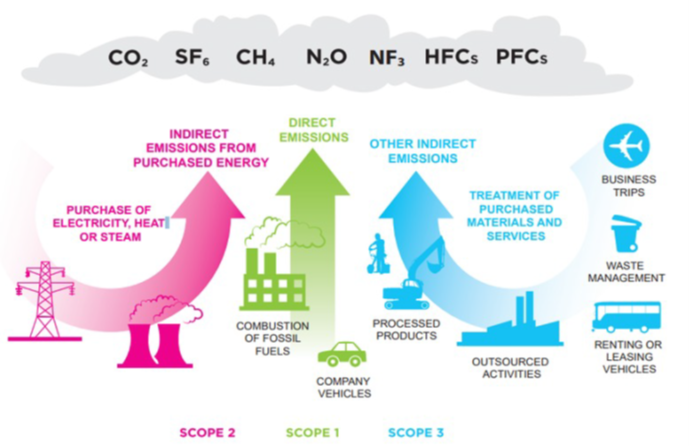
\includegraphics[width=\textwidth,keepaspectratio]{./Carbon_Accounting_Scopes.png}
\caption{Κατηγορίες Εκπομπών}
\end{figure}

\subsection{Κατηγορία 1 (Scope 1): Άμεσες
εκπομπές}\label{ux3baux3b1ux3c4ux3b7ux3b3ux3bfux3c1ux3afux3b1-1-scope-1-ux3acux3bcux3b5ux3c3ux3b5ux3c2-ux3b5ux3baux3c0ux3bfux3bcux3c0ux3adux3c2}

Οι εκπομπές Scope 1 προέρχονται από πηγές που ανήκουν ή ελέγχονται άμεσα
από τον οργανισμό. Για μια ναυτιλιακή εταιρεία όπως η Maersk, αυτές
περιλαμβάνουν κατά κύριο λόγο την καύση καυσίμων στα ιδιόκτητα πλοία,
τις σταθερές εγκαταστάσεις (γραφεία, αποθήκες, τερματικοί σταθμοί που
λειτουργεί η ίδια η εταιρεία), καθώς και τα οχήματα που ανήκουν στον
οργανισμό {[}GHG Protocol Corporate Standard, 2004{]}.

\subsection{Κατηγορία 2 (Scope 2): Έμμεσες εκπομπές από
ενέργεια}\label{ux3baux3b1ux3c4ux3b7ux3b3ux3bfux3c1ux3afux3b1-2-scope-2-ux3adux3bcux3bcux3b5ux3c3ux3b5ux3c2-ux3b5ux3baux3c0ux3bfux3bcux3c0ux3adux3c2-ux3b1ux3c0ux3cc-ux3b5ux3bdux3adux3c1ux3b3ux3b5ux3b9ux3b1}

Οι εκπομπές Scope 2 αφορούν τις έμμεσες εκπομπές που συνδέονται με την
αγορά ηλεκτρικής ενέργειας, θερμότητας, ατμού ή ψύξης από τρίτους
παρόχους. Οι εκπομπές παράγονται φυσικά εκτός του οργανισμού --- στο
σταθμό παραγωγής ενέργειας ή στο σύστημα τηλεθέρμανσης --- αλλά
αποδίδονται λογιστικά στον καταναλωτή. Στη Maersk, τυπικές πηγές Scope 2
είναι η κατανάλωση ηλεκτρισμού στα κεντρικά γραφεία και στους λιμενικούς
τερματικούς σταθμούς. Σύμφωνα με το GHGP Scope 2 Guidance (2015),
διακρίνονται δύο μέθοδοι υπολογισμού: η \emph{location-based} (βάσει
μέσου συντελεστή εκπομπών ηλεκτρισμού της αγοράς) και η
\emph{market-based} (βάσει συμβολαίων αγοράς ανανεώσιμης ενέργειας ή
εγγυήσεων προέλευσης) {[}GHG Protocol Scope 2 Guidance, 2015{]}.

\subsection{Κατηγορία 3 (Scope 3): Εκπομπές αλυσίδας
αξίας}\label{ux3baux3b1ux3c4ux3b7ux3b3ux3bfux3c1ux3afux3b1-3-scope-3-ux3b5ux3baux3c0ux3bfux3bcux3c0ux3adux3c2-ux3b1ux3bbux3c5ux3c3ux3afux3b4ux3b1ux3c2-ux3b1ux3beux3afux3b1ux3c2}

Το Scope 3 καλύπτει το σύνολο των έμμεσων εκπομπών που προκύπτουν στην
αλυσίδα αξίας (upstream και downstream) και δεν εντάσσονται στο Scope 2.
Σύμφωνα με το \emph{Scope 3 Standard} {[}GHG Protocol Scope 3 Standard,
2011{]}, ορίζονται 15 κατηγορίες, εκ των οποίων οι πλέον σχετικές για τη
ναυτιλία είναι:

\begin{itemize}
\tightlist
\item
  \textbf{Κατηγορία 1} (Αγορασθέντα αγαθά και υπηρεσίες): π.χ. αγορά
  καυσίμων, εξοπλισμού.
\item
  \textbf{Κατηγορία 4} (Μεταφορά και διανομή upstream): μεταφορές που
  αναθέτει η εταιρεία σε τρίτους.
\item
  \textbf{Κατηγορία 7} (Μεταφορά εργαζομένων): μετακινήσεις πληρωμάτων.
\item
  \textbf{Κατηγορία 11} (Χρήση πωληθέντων προϊόντων): εκπομπές στις
  μεταφορές που παρέχει ως υπηρεσία.
\end{itemize}

Ένα ειδικά σημαντικό ζήτημα για τη Maersk αφορά τα \textbf{ναυλωμένα
πλοία} (chartered vessels). Όταν η εταιρεία ναυλώνει πλοία από τρίτους,
η καύση καυσίμου στα πλοία αυτά δεν εμπίπτει στο Scope 1 (δεν υπάρχει
ιδιοκτησία ή λειτουργικός έλεγχος ανάλογα με τον επιλεγμένο ορισμό
ορίου), αλλά συνήθως στο Scope 3 κατηγορία 4 ή 7, ανάλογα με τον τύπο
ναύλωσης και τη μέθοδο οριοθέτησης (\emph{financial control}
vs.~\emph{operational control approach}). Αυτή η διάκριση έχει
σημαντικές επιπτώσεις στον σχεδιασμό συστημάτων καταγραφής, καθώς για τα
ιδιόκτητα πλοία είναι διαθέσιμα αναλυτικά δεδομένα κατανάλωσης καυσίμου,
ενώ για τα ναυλωμένα συχνά απαιτείται εκτίμηση βάσει μέσης κατανάλωσης
κλάσης πλοίου ή τύπου διαδρομής.

Αξίζει να σημειωθεί ότι ο Πάγκος Εργασίας Εκπομπών, στην παρούσα φάση
του (2025), καλύπτει εκπομπές Scope 1 και Scope 3, ενώ η ενσωμάτωση του
Scope 2 βρίσκεται σε εξέλιξη (βλ. Κεφ. 5).

\begin{center}\rule{0.5\linewidth}{0.5pt}\end{center}

\section{3.3 Μεθοδολογίες
Μέτρησης}\label{ux3bcux3b5ux3b8ux3bfux3b4ux3bfux3bbux3bfux3b3ux3afux3b5ux3c2-ux3bcux3adux3c4ux3c1ux3b7ux3c3ux3b7ux3c2}

Ανεξαρτήτως κατηγορίας (scope), για τον ποσοτικό υπολογισμό εκπομπών
υπάρχουν τρεις βασικές μεθοδολογικές προσεγγίσεις, οι οποίες διαφέρουν
ως προς τον τύπο δεδομένων εισόδου, την ακρίβεια που παρέχουν και το
κόστος εφαρμογής τους. Το GHGP Scope 3 Standard αναγνωρίζει ρητά και τις
τρεις {[}GHG Protocol Scope 3 Standard, 2011{]}.

\subsection{3.3.1 Μεθοδολογία βάσει κόστους
(Cost-based)}\label{ux3bcux3b5ux3b8ux3bfux3b4ux3bfux3bbux3bfux3b3ux3afux3b1-ux3b2ux3acux3c3ux3b5ux3b9-ux3baux3ccux3c3ux3c4ux3bfux3c5ux3c2-cost-based}

Στη μεθοδολογία βάσει κόστους, οι εκπομπές υπολογίζονται
πολλαπλασιάζοντας την οικονομική αξία (δαπάνη) μιας αγοράς ή
δραστηριότητας επί έναν οικονομικό συντελεστή εκπομπών
(\emph{Environmentally Extended Input-Output}, EEIO factor),
εκπεφρασμένο σε kgCO₂e ανά νομισματική μονάδα δαπάνης.

Οι συντελεστές EEIO προέρχονται από εθνικούς ή κλαδικούς πίνακες
εισόδου-εξόδου και αντικατοπτρίζουν τον μέσο εκπομπτόμενο άνθρακα ανά
μονάδα οικονομικής αξίας για τον εκάστοτε κλάδο. Η προσέγγιση αυτή έχει
το πλεονέκτημα της απλότητας: χρειάζεται μόνο τα τιμολόγια αγορών, χωρίς
ανάγκη φυσικών μετρήσεων.

Ωστόσο, τα μειονεκτήματά της είναι σημαντικά. Πρώτον, οι EEIO
συντελεστές αντικατοπτρίζουν μέσους όρους ολόκληρων κλάδων, με
αποτέλεσμα ανακρίβειες όταν ο συγκεκριμένος προμηθευτής ή δραστηριότητα
αποκλίνει από τον μέσο. Δεύτερον, τα αποτελέσματα είναι ευαίσθητα στις
διακυμάνσεις τιμών αγοράς: αύξηση τιμής καυσίμου οδηγεί τεχνηέντως σε
αύξηση εκτιμώμενων εκπομπών, ακόμα και αν η πραγματική κατανάλωση
παρέμεινε σταθερή. Για λόγους αυτούς, η μεθοδολογία βάσει κόστους
συνιστάται μόνο ως \emph{fallback} σε περιπτώσεις απουσίας πρωτογενών
δεδομένων {[}GHG Protocol Scope 3 Standard, 2011{]}.

\subsection{3.3.2 Μεθοδολογία βάσει δραστηριότητας
(Activity-based)}\label{ux3bcux3b5ux3b8ux3bfux3b4ux3bfux3bbux3bfux3b3ux3afux3b1-ux3b2ux3acux3c3ux3b5ux3b9-ux3b4ux3c1ux3b1ux3c3ux3c4ux3b7ux3c1ux3b9ux3ccux3c4ux3b7ux3c4ux3b1ux3c2-activity-based}

Στη μεθοδολογία βάσει δραστηριότητας, οι εκπομπές υπολογίζονται
πολλαπλασιάζοντας ένα μέτρο φυσικής δραστηριότητας (\emph{activity
data}) επί έναν εξειδικευμένο συντελεστή εκπομπών:

\textbf{Εκπομπές = Δεδομένα Δραστηριότητας × Συντελεστής Εκπομπών}

Στη ναυτιλία, τυπικά παραδείγματα είναι:

\begin{itemize}
\tightlist
\item
  \textbf{Κατανάλωση καυσίμου} (τόνοι καυσίμου) × \textbf{συντελεστής
  εκπομπών καυσίμου} (kgCO₂e/τόνο) --- η πλέον ακριβής μέθοδος για
  εκπομπές Scope 1.
\item
  \textbf{Τονοχιλιόμετρα} (tonne-km) × \textbf{εκπομπές ανά tonne-km}
  (gCO₂e/tonne-km) --- χρήσιμο για κατανομή εκπομπών ανά φορτίο.
\item
  \textbf{Ναυτικά μίλια} × \textbf{κατανάλωση καυσίμου ανά μίλι} για
  συγκεκριμένο τύπο πλοίου.
\end{itemize}

Οι συντελεστές εκπομπών για διαφορετικά καύσιμα (HFO, VLSFO, MGO, LNG,
βιοκαύσιμα κ.λπ.) δημοσιεύονται από διεθνείς οργανισμούς όπως ο IMO, η
Ευρωπαϊκή Επιτροπή (για τους σκοπούς EU ETS) και διάφοροι φορείς
πιστοποίησης. Η μεθοδολογία αυτή παρέχει σημαντικά υψηλότερη ακρίβεια
και επαληθευσιμότητα σε σύγκριση με την cost-based, αλλά απαιτεί
αναλυτική καταγραφή φυσικών δεδομένων δραστηριότητας --- κάτι που
αποτελεί το πλέον απαιτητικό κομμάτι από πλευράς συλλογής και ποιοτικού
ελέγχου δεδομένων. Στην περίπτωση της Maersk, αυτό σημαίνει άντληση
δεδομένων κατανάλωσης καυσίμου από ποικίλα πληροφοριακά συστήματα
πλοίων, τα οποία χρησιμοποιούν διαφορετικές μορφές και σχήματα δεδομένων
(βλ. Κεφ. 5).

\subsection{3.3.3 Υβριδική μεθοδολογία
(Hybrid)}\label{ux3c5ux3b2ux3c1ux3b9ux3b4ux3b9ux3baux3ae-ux3bcux3b5ux3b8ux3bfux3b4ux3bfux3bbux3bfux3b3ux3afux3b1-hybrid}

Η υβριδική μεθοδολογία συνδυάζει τις δύο προηγούμενες: χρησιμοποιεί
activity-based δεδομένα όπου είναι διαθέσιμα, και συμπληρώνει τα κενά με
cost-based εκτιμήσεις. Αυτή η προσέγγιση συνιστάται ρητά από το GHGP ως
η προτιμώμενη μέθοδος για τον υπολογισμό Scope 3 εκπομπών, καθώς
μεγιστοποιεί την ακρίβεια στους τομείς όπου υπάρχουν δεδομένα, ενώ
διατηρεί πλήρη κάλυψη όλων των κατηγοριών {[}GHG Protocol Scope 3
Standard, 2011{]}.

Η υβριδική μεθοδολογία είναι αυτή που επιλέχθηκε να υλοποιηθεί στον
Πάγκο Εργασίας Εκπομπών της Maersk. Στην πράξη, αυτό σημαίνει ότι για
κάθε αποστολή (shipment) το σύστημα προσπαθεί πρώτα να χρησιμοποιήσει
πραγματικά δεδομένα κατανάλωσης καυσίμου (activity-based), και όταν αυτά
δεν είναι διαθέσιμα --- π.χ. για ναυλωμένα πλοία ή για παλαιότερα
δεδομένα πριν την ενεργοποίηση τροφοδοσιών δεδομένων --- χρησιμοποιεί
εκτιμήσεις βάσει τύπου πλοίου, χωρητικότητας και αποστάσεων. Η
λεπτομερής υλοποίηση αυτής της λογικής περιγράφεται στο Κεφάλαιο 5.5.

\begin{center}\rule{0.5\linewidth}{0.5pt}\end{center}

\section{3.4 TTW έναντι WTW: Όρια του συστήματος
εκπομπών}\label{ttw-ux3adux3bdux3b1ux3bdux3c4ux3b9-wtw-ux3ccux3c1ux3b9ux3b1-ux3c4ux3bfux3c5-ux3c3ux3c5ux3c3ux3c4ux3aeux3bcux3b1ux3c4ux3bfux3c2-ux3b5ux3baux3c0ux3bfux3bcux3c0ux3ceux3bd}

Ένα κρίσιμο θεωρητικό ζήτημα στη λογιστική εκπομπών καυσίμων αφορά τον
ορισμό των ορίων του συστήματος: πού «ξεκινά» και πού «τελειώνει» η
αλυσίδα που μετράμε;

\subsection{Tank-to-Wake (TTW)}\label{tank-to-wake-ttw}

Η προσέγγιση \textbf{Tank-to-Wake} (TTW), μετρά αποκλειστικά τις
εκπομπές που προκύπτουν κατά την καύση του καυσίμου στη μηχανή του
οχήματος ή πλοίου. Είναι το παραδοσιακό μέτρο που χρησιμοποιείται για
τον καθορισμό κατανάλωσης καυσίμου και εκπομπών Scope 1, και εκφράζεται
συνήθως σε gCO₂/kWh ή gCO₂/tonne-nm.

Το TTW αποτυπώνει εκπομπές που είναι άμεσα μετρήσιμες και επαληθεύσιμες.
Ωστόσο, αυτή η προσέγγιση παρουσιάζει σημαντικό μειονέκτημα όταν
συγκρίνονται διαφορετικά καύσιμα: ένα πλοίο που χρησιμοποιεί πράσινο
υδρογόνο ή βιοκαύσιμα έχει TTW εκπομπές πολύ χαμηλότερες (ή μηδενικές,
για καύσιμα με βιογενές CO₂), αλλά η παραγωγή τους μπορεί να ήταν
ενεργειακά εντατική.

\subsection{Well-to-Wake (WTW)}\label{well-to-wake-wtw}

Η προσέγγιση \textbf{Well-to-Wake} (WTW) επεκτείνει τα όρια του
συστήματος ώστε να συμπεριλαμβάνει επίσης τις εκπομπές που συνδέονται με
την εξόρυξη, επεξεργασία, μεταφορά και διανομή του καυσίμου
(\emph{Well-to-Tank}, WTT). Δηλαδή:

\textbf{WTW = WTT (Well-to-Tank) + TTW (Tank-to-Wake)}

Η WTW προσέγγιση είναι απαραίτητη για μια ολοκληρωμένη σύγκριση
εναλλακτικών καυσίμων. Για παράδειγμα:

\begin{itemize}
\tightlist
\item
  Το \textbf{LNG} (liquefied natural gas) έχει χαμηλότερες εκπομπές CO₂
  TTW σε σχέση με το HFO, αλλά η παραγωγή και υγροποίησή του συνεπάγεται
  σημαντικές WTT εκπομπές, και η διαφυγή μεθανίου (CH₄) κατά τη
  φόρτωση/εκφόρτωση (\emph{methane slip}) έχει υψηλό GWP.
\item
  Τα \textbf{βιώσιμα βιοκαύσιμα} (π.χ. FAME από απόβλητα λίπη) έχουν
  σχεδόν μηδενικό TTW CO₂ (βιογενής άνθρακας), αλλά το πλήρες WTW
  αποτύπωμά τους εξαρτάται κρίσιμα από τη διαδρομή παραγωγής.
\item
  Το \textbf{πράσινο υδρογόνο} από ηλεκτρόλυση με ανανεώσιμη ενέργεια
  έχει μηδενικές TTW εκπομπές, αλλά η παραγωγή του απαιτεί σημαντικές
  ποσότητες ηλεκτρικής ενέργειας.
\end{itemize}

Η ευρωπαϊκή νομοθεσία κινείται ρητά προς τη WTW προσέγγιση: ο Κανονισμός
\textbf{FuelEU Maritime} (Κανονισμός (ΕΕ) 2023/1805), που τέθηκε σε ισχύ
από 1 Ιανουαρίου 2025, χρησιμοποιεί ένταση εκπομπών ΘΚ σε WTW βάση για
τον ορισμό στόχων μείωσης, σε αντίθεση με τον Κανονισμό EU ETS Maritime
που βασίζεται σε TTW μετρήσεις {[}Κανονισμός (ΕΕ) 2023/1805, FuelEU
Maritime{]}.

Στον Πάγκο Εργασίας Εκπομπών, η διάκριση TTW/WTW αποτελεί βασική
παράμετρο του μοντέλου δεδομένων: κάθε αποτέλεσμα εκπομπών μπορεί να
παρουσιαστεί και στις δύο βάσεις, ώστε να ανταποκρίνεται στις
διαφορετικές κανονιστικές και εμπορικές απαιτήσεις (βλ. Κεφ. 5.3 και
6.3).

\begin{center}\rule{0.5\linewidth}{0.5pt}\end{center}

\section{3.5 Mass Balance και
Book-and-Claim}\label{mass-balance-ux3baux3b1ux3b9-book-and-claim}

Καθώς τα εναλλακτικά καύσιμα χαμηλού άνθρακα επεκτείνονται στον κλάδο
της ναυτιλίας, προκύπτει ένα θεμελιώδες λογιστικό ζήτημα: πώς
αποδίδονται οι περιβαλλοντικές ιδιότητες ενός καυσίμου όταν η φυσική ροή
του καυσίμου δεν ακολουθεί πάντα τη λογιστική αναφορά;

\subsection{Φυσική ροή έναντι λογιστικής
ροής}\label{ux3c6ux3c5ux3c3ux3b9ux3baux3ae-ux3c1ux3bfux3ae-ux3adux3bdux3b1ux3bdux3c4ux3b9-ux3bbux3bfux3b3ux3b9ux3c3ux3c4ux3b9ux3baux3aeux3c2-ux3c1ux3bfux3aeux3c2}

Σε ένα ιδανικό σύστημα, κάθε τόνος βιοκαυσίμου που αγοράζεται από έναν
πελάτη θα χρησιμοποιείτο στο συγκεκριμένο πλοίο που μεταφέρει το φορτίο
του. Στην πράξη, αυτό είναι συχνά αδύνατο λόγω περιορισμών εφοδιαστικής
αλυσίδας (εναλλακτικά καύσιμα δεν είναι διαθέσιμα σε όλα τα λιμάνια),
τεχνικών περιορισμών (συμβατότητα μηχανών) και οικονομικής σκοπιμότητας.
Δύο θεωρητικά πλαίσια αντιμετωπίζουν αυτή την πρακτική πρόκληση: το
\emph{mass balance} και το \emph{book-and-claim}.

\subsection{Mass Balance (Ισοζύγιο
μάζας)}\label{mass-balance-ux3b9ux3c3ux3bfux3b6ux3cdux3b3ux3b9ux3bf-ux3bcux3acux3b6ux3b1ux3c2}

Το \textbf{mass balance} (ισοζύγιο μάζας) είναι μια μέθοδος αλυσίδας
επιμέλειας (\emph{chain-of-custody}) που επιτρέπει τον εικονικό
διαχωρισμό των βιώσιμων ιδιοτήτων ενός καυσίμου εντός ενός φυσικά
ανάμεικτου συστήματος, υπό την προϋπόθεση ότι οι εισροές και εκροές
ιχνηλατούνται αυστηρά ανά καθορισμένο χρονικό παράθυρο και γεωγραφικό
πεδίο {[}ISCC System Document ISCC-203, 2023{]}.

Στην πράξη: μια εταιρεία μπορεί να αναμείξει βιώσιμο καύσιμο με
συμβατικό σε κοινή υποδομή (π.χ. αγωγό, αποθήκη λιμανιού), αρκεί να
διατηρεί ακριβή καταγραφή της ποσότητας βιώσιμου καυσίμου που εισέρχεται
στο σύστημα. Στη συνέχεια, οι «βιώσιμες μονάδες» μπορούν να παραδοθούν
λογιστικά σε πελάτες που αγόρασαν βιώσιμο καύσιμο, ακόμα και αν στο
πλοίο τους φορτώθηκε φυσικά μίγμα.

Το mass balance αποτελεί την επίσημη μέθοδο που αναγνωρίζεται από τα
πλέον διαδεδομένα πιστοποιητικά βιωσιμότητας καυσίμων,
συμπεριλαμβανομένων του \textbf{ISCC EU} και \textbf{ISCC Plus}, στο
πλαίσιο της Ευρωπαϊκής Οδηγίας για Ανανεώσιμες Πηγές Ενέργειας II (RED
II, Οδηγία 2018/2001/ΕΕ) {[}Ευρωπαϊκή Επιτροπή, RED II, 2018{]}.

\subsection{Book-and-Claim (Αναφορά αποσυνδεδεμένη από φυσική
ροή)}\label{book-and-claim-ux3b1ux3bdux3b1ux3c6ux3bfux3c1ux3ac-ux3b1ux3c0ux3bfux3c3ux3c5ux3bdux3b4ux3b5ux3b4ux3b5ux3bcux3adux3bdux3b7-ux3b1ux3c0ux3cc-ux3c6ux3c5ux3c3ux3b9ux3baux3ae-ux3c1ux3bfux3ae}

Το \textbf{book-and-claim} (λογιστική και απαίτηση) αντιπροσωπεύει ένα
πλαίσιο στο οποίο οι περιβαλλοντικές ιδιότητες ενός καυσίμου
αποσυνδέονται πλήρως από τη φυσική παράδοσή του. Ο πελάτης «αγοράζει»
ένα πιστωτικό περιβαλλοντικής αξίας (\emph{claim}) που αντιστοιχεί σε
συγκεκριμένη ποσότητα βιώσιμου καυσίμου που έχει χρησιμοποιηθεί κάπου
στο σύστημα, χωρίς αυτό να έχει φορτωθεί στο συγκεκριμένο πλοίο του
πελάτη.

Αναλογικά παραδείγματα από άλλους κλάδους:

\begin{itemize}
\tightlist
\item
  \textbf{Πιστοποιητικά Ανανεώσιμης Ενέργειας} (\emph{Renewable Energy
  Certificates}, RECs / \emph{Guarantees of Origin}): ο αγοραστής
  κατανάλωσε ηλεκτρισμό από το δίκτυο αλλά έχει αγοράσει ισόποσες
  ανανεώσιμες μονάδες.
\item
  \textbf{Βιώσιμα Αεροπορικά Καύσιμα} (\emph{Sustainable Aviation Fuel},
  SAF): το book-and-claim χρησιμοποιείται ευρέως στην αεροπορία για
  επιτρεπόμενη αναφορά SAF χρήσης χωρίς φυσική ιχνηλάτηση ανά πτήση.
\end{itemize}

Στη ναυτιλία, το book-and-claim εισάγεται σταδιακά, ιδίως για προϊόντα
ECO (\emph{Eco-delivery}). Η Maersk χρησιμοποιεί book-and-claim για το
ECO Delivery Ocean (ECOv1/ECOv2): ένας πελάτης αγοράζει μειωμένες
εκπομπές για τη διαδρομή του, και αυτές αντισταθμίζονται από πραγματική
χρήση βιώσιμου καυσίμου σε κάποιο άλλο φορτίο στο σύστημα {[}βλ. Κεφ.
6.4 για πλήρη ανάλυση της υλοποίησης μέσω Energy Bank{]}.

\subsection{Πλεονεκτήματα και
περιορισμοί}\label{ux3c0ux3bbux3b5ux3bfux3bdux3b5ux3baux3c4ux3aeux3bcux3b1ux3c4ux3b1-ux3baux3b1ux3b9-ux3c0ux3b5ux3c1ux3b9ux3bfux3c1ux3b9ux3c3ux3bcux3bfux3af}

Και οι δύο μέθοδοι απαιτούν αυστηρή διαφάνεια και ελεγξιμότητα. Το mass
balance διατηρεί ισχυρότερη φυσική σύνδεση και είναι η μέθοδος που
αναγνωρίζεται για κανονιστικούς σκοπούς (RED II, EU ETS). Το
book-and-claim προσφέρει μεγαλύτερη εμπορική ευελιξία αλλά εγείρει
ερωτήματα αξιοπιστίας αν δεν υποστηρίζεται από επαρκή τεκμηρίωση.
Κρίσιμη προϋπόθεση και για τα δύο πλαίσια είναι η εφαρμογή ενός
συστήματος πληροφορικής ικανού να παρακολουθεί σε πραγματικό χρόνο τόσο
την κατανάλωση πραγματικών καυσίμων ανά πλοίο, όσο και τα διαθέσιμα
πιστωτικά εναλλακτικού καυσίμου --- ακριβώς ο ρόλος του Energy Bank στον
Πάγκο Εργασίας Εκπομπών (βλ. Κεφ. 6.3).

\begin{center}\rule{0.5\linewidth}{0.5pt}\end{center}

\section{3.6 Πρότυπα και
Πιστοποιήσεις}\label{ux3c0ux3c1ux3ccux3c4ux3c5ux3c0ux3b1-ux3baux3b1ux3b9-ux3c0ux3b9ux3c3ux3c4ux3bfux3c0ux3bfux3b9ux3aeux3c3ux3b5ux3b9ux3c2}

Πέραν του GHGP και του ISO 14064 που αναλύθηκαν στην ενότητα 3.1, ο
τομέας της ναυτιλίας και της εφοδιαστικής αλυσίδας διαθέτει σειρά
εξειδικευμένων προτύπων και πλαισίων πιστοποίησης που είναι άμεσα
σχετικά με τον Πάγκο Εργασίας Εκπομπών.

\subsection{ISCC (International Sustainability and Carbon
Certification)}\label{iscc-international-sustainability-and-carbon-certification}

Το \textbf{ISCC} είναι ένα διεθνές σύστημα πιστοποίησης βιωσιμότητας και
ανθρακικής ουδετερότητας για βιομάζα, βιοκαύσιμα, βιογενή υγρά,
ανακυκλωμένα καύσιμα αεροσκαφών (SAF) και ανανεώσιμα καύσιμα μη
βιολογικής προέλευσης (RFNBO). Η έκδοση \textbf{ISCC EU} αναγνωρίζεται
επίσημα από την Ευρωπαϊκή Επιτροπή στο πλαίσιο της Οδηγίας RED II
(2018/2001/ΕΕ) για τη θεσμική αναγνώριση βιώσιμων καυσίμων {[}ISCC
System Document ISCC-203, 2023{]}.

Η πιστοποίηση ISCC βασίζεται σε αλυσίδα επιμέλειας με τη μέθοδο mass
balance: κάθε φορέας στην αλυσίδα εφοδιασμού (παραγωγός, επεξεργαστής,
διανομέας) πρέπει να πιστοποιηθεί ανεξάρτητα από διαπιστευμένο φορέα
ελέγχου. Για τη Maersk, η πιστοποίηση ISCC των προμηθευτών βιοκαυσίμων
αποτελεί προαπαιτούμενο για τη διάθεση ECO προϊόντων, καθώς επιτρέπει
την τεκμηριωμένη αναγνώριση μειωμένου ανθρακικού αποτυπώματος (βλ. Κεφ.
6.4).

\subsection{SBTi Maritime (Science Based Targets
initiative)}\label{sbti-maritime-science-based-targets-initiative}

Η \textbf{SBTi} είναι πρωτοβουλία κοινής διαχείρισης από τον CDP, το UN
Global Compact, το WRI και το WWF, που επιτρέπει σε εταιρείες να θέτουν
επιστημονικά βασισμένους στόχους μείωσης εκπομπών (\emph{science-based
targets}) συμβατούς με την ανάγκη περιορισμού της θερμοκρασιακής αύξησης
στον 1,5°C σύμφωνα με τη Συμφωνία του Παρισιού {[}SBTi Corporate Manual,
2023{]}.

Η SBTi διαθέτει εξειδικευμένο εταιρικό εγχειρίδιο που ορίζει τους
κανόνες για όλους τους τομείς, ενώ εκπονεί τομεακές κατευθυντήριες
γραμμές. Για τη ναυτιλία, το \emph{SBTi Maritime Guidance} (σε φάση
πιλοτικής εφαρμογής) ορίζει μεθοδολογία για τον καθορισμό αποθεμάτων
άνθρακα (\emph{carbon budget}) ανά εταιρεία βάσει μεριδίου στόλου και
μεριδίου αγοράς. Η Maersk έχει δεσμευτεί σε SBTi-aligned στόχους
μείωσης, γεγονός που αυξάνει την ανάγκη για ακριβή και επαληθεύσιμη
καταγραφή εκπομπών σε κεντρικό σύστημα.

\subsection{GLEC Framework (Global Logistics Emissions
Council)}\label{glec-framework-global-logistics-emissions-council}

Το \textbf{GLEC Framework} (έκδοση 3, 2023) είναι η κλαδική μεθοδολογία
για τον υπολογισμό και την αναφορά εκπομπών σε διαφορετικές μορφές
εφοδιαστικής αλυσίδας. Αναπτύχθηκε από το \emph{Smart Freight Centre}
και έχει λάβει την αναγνώριση ευρέος φάσματος φορέων του κλάδου {[}GLEC
Framework v3.0, Smart Freight Centre, 2023{]}. Βασίζεται στις αρχές του
GHGP και του EN 16258, εισάγοντας ωστόσο εξειδικευμένες μεθοδολογίες για
κάθε κατηγορία μεταφοράς (οδική, σιδηροδρομική, θαλάσσια, εναέρια).

Ειδικότερα για τη θαλάσσια μεταφορά, το GLEC v3 παρέχει:

\begin{itemize}
\tightlist
\item
  Προκαθορισμένους συντελεστές εκπομπών ανά τύπο πλοίου και τύπο φορτίου
  (\emph{default emission factors}).
\item
  Μεθοδολογία κατανομής εκπομπών σε επίπεδο container (φορτίου),
  διακρίνοντας μεταξύ 20' (TEU) και 40' (FFE) container, dry και reefer.
\item
  Κανόνες για τον χειρισμό μικτών φορτίων και συνδυαστικών διαδρομών.
\end{itemize}

Η Maersk ευθυγραμμίζεται με το GLEC Framework για την παροχή εκπομπών
ανά αποστολή στους πελάτες, διασφαλίζοντας ότι τα δεδομένα που παρέχει ο
Πάγκος Εργασίας Εκπομπών είναι συγκρίσιμα με εκείνα άλλων μεταφορέων που
ακολουθούν το ίδιο πλαίσιο.

\subsection{CDP και ISO 14001}\label{cdp-ux3baux3b1ux3b9-iso-14001}

Το \textbf{CDP} (\emph{Carbon Disclosure Project}) είναι εθελοντικό
πλαίσιο γνωστοποίησης κλιματικού αποτυπώματος, χρηματοοικονομικών
κινδύνων και στρατηγικών διαχείρισης, στο οποίο εκατοντάδες εταιρείες
αναφέρουν εκπομπές, στόχους και πρακτικές. Η Maersk συμμετέχει ετήσια
στην αξιολόγηση CDP Climate.

Το \textbf{ISO 14001} είναι διεθνές πρότυπο για συστήματα
περιβαλλοντικής διαχείρισης (\emph{Environmental Management System},
EMS), το οποίο ορίζει πλαίσιο για τον εντοπισμό, την παρακολούθηση και
τη βελτίωση των περιβαλλοντικών επιπτώσεων ενός οργανισμού. Αν και δεν
είναι εξειδικευμένο για εκπομπές ΘΚ, αποτελεί συνήθη οργανωτική βάση που
υποστηρίζει τις διαδικασίες GHGP/ISO 14064.

\subsection{Σύνοψη κανονιστικού και προτυπικού
πλαισίου}\label{ux3c3ux3cdux3bdux3bfux3c8ux3b7-ux3baux3b1ux3bdux3bfux3bdux3b9ux3c3ux3c4ux3b9ux3baux3bfux3cd-ux3baux3b1ux3b9-ux3c0ux3c1ux3bfux3c4ux3c5ux3c0ux3b9ux3baux3bfux3cd-ux3c0ux3bbux3b1ux3b9ux3c3ux3afux3bfux3c5}

Ο παρακάτω πίνακας συνοψίζει τα βασικά πρότυπα και πλαίσια που
επηρεάζουν τον σχεδιασμό του Πάγκου Εργασίας Εκπομπών:

{\def\LTcaptype{} % do not increment counter
\begin{longtable}[]{@{}
  >{\raggedright\arraybackslash}p{(\linewidth - 4\tabcolsep) * \real{0.3333}}
  >{\raggedright\arraybackslash}p{(\linewidth - 4\tabcolsep) * \real{0.3333}}
  >{\raggedright\arraybackslash}p{(\linewidth - 4\tabcolsep) * \real{0.3333}}@{}}
\toprule\noalign{}
\begin{minipage}[b]{\linewidth}\raggedright
Πρότυπο / Πλαίσιο
\end{minipage} & \begin{minipage}[b]{\linewidth}\raggedright
Τύπος
\end{minipage} & \begin{minipage}[b]{\linewidth}\raggedright
Κύρια σχέση με το σύστημα
\end{minipage} \\
\midrule\noalign{}
\endhead
\bottomrule\noalign{}
\endlastfoot
GHG Protocol Corporate Standard (2004) & Μεθοδολογικό & Ορισμός Scopes
1/2/3, μεθοδολογίες \\
GHG Protocol Scope 3 Standard (2011) & Μεθοδολογικό & Scope 3
κατηγορίες, υβριδική μέθοδος \\
ISO 14064-1 (2018) & Πιστοποίηση & Επαλήθευση οργανωτικής απογραφής \\
EN 16258 (2012) & Κανονιστικό & Εκπομπές μεταφοράς εμπορευμάτων \\
ISCC EU & Πιστοποίηση & Τεκμηρίωση βιώσιμων καυσίμων, ECO products \\
GLEC Framework v3 (2023) & Κλαδικό & Κατανομή εκπομπών ανά container \\
SBTi Maritime Guidance & Στρατηγικό & Ευθυγράμμιση εταιρικών στόχων \\
FuelEU Maritime (2023/1805) & Νομοθετικό & WTW εντάσεις εκπομπών από
2025 \\
EU ETS Maritime & Νομοθετικό & TTW CO₂ αναφορά, αγορά δικαιωμάτων \\
\end{longtable}
}

Το σύνολο αυτό των προτύπων και κανονισμών καθορίζει πολύπλοκες, συχνά
αλληλεπικαλυπτόμενες απαιτήσεις, οι οποίες πρέπει να ικανοποιούνται
ταυτόχρονα από ένα ενιαίο σύστημα πληροφορικής. Στο επόμενο κεφάλαιο
παρουσιάζεται ο τρόπος με τον οποίο ο Πάγκος Εργασίας Εκπομπών
οργανώθηκε για να ανταποκρίνεται σε αυτές τις ετερογενείς απαιτήσεις ως
ενιαία πλατφόρμα (βλ. Κεφ. 4).

\begin{center}\rule{0.5\linewidth}{0.5pt}\end{center}

\subsection{Βιβλιογραφικές αναφορές
κεφαλαίου}\label{ux3b2ux3b9ux3b2ux3bbux3b9ux3bfux3b3ux3c1ux3b1ux3c6ux3b9ux3baux3adux3c2-ux3b1ux3bdux3b1ux3c6ux3bfux3c1ux3adux3c2-ux3baux3b5ux3c6ux3b1ux3bbux3b1ux3afux3bfux3c5}

\begin{itemize}
\tightlist
\item
  {[}GHG Protocol Corporate Standard, 2004{]} World Resources Institute
  \& WBCSD. \emph{A Corporate Accounting and Reporting Standard},
  Revised Edition. Washington DC: WRI/WBCSD, 2004.
\item
  {[}GHG Protocol Scope 2 Guidance, 2015{]} World Resources Institute.
  \emph{Scope 2 Accounting Guidance}. WRI, 2015.
\item
  {[}GHG Protocol Scope 3 Standard, 2011{]} World Resources Institute \&
  WBCSD. \emph{Corporate Value Chain (Scope 3) Accounting and Reporting
  Standard}. WRI/WBCSD, 2011.
\item
  {[}IPCC AR5, 2013{]} IPCC. \emph{Climate Change 2013: The Physical
  Science Basis}. Cambridge: Cambridge University Press, 2013.
\item
  {[}UNFCCC, 2012{]} UNFCCC. \emph{Doha Amendment to the Kyoto
  Protocol}. 2012.
\item
  {[}ISO 14064-1, 2018{]} International Organization for
  Standardization. \emph{ISO 14064-1:2018 --- Greenhouse gases --- Part
  1: Specification with guidance at the organization level}. Geneva:
  ISO, 2018.
\item
  {[}CEN EN 16258, 2012{]} European Committee for Standardization.
  \emph{EN 16258:2012 --- Methodology for calculation and declaration of
  energy consumption and GHG emissions of transport services}. Brussels:
  CEN, 2012.
\item
  {[}ISCC System Document ISCC-203, 2023{]} International Sustainability
  and Carbon Certification. \emph{ISCC System Document ISCC-203:
  Requirements for the Supply Chain}. Cologne: ISCC, 2023.
\item
  {[}GLEC Framework v3.0, 2023{]} Smart Freight Centre. \emph{Global
  Logistics Emissions Council Framework for Logistics Emissions
  Accounting and Reporting, Version 3.0}. Amsterdam: Smart Freight
  Centre, 2023.
\item
  {[}SBTi Corporate Manual, 2023{]} Science Based Targets initiative.
  \emph{SBTi Corporate Manual}. London: SBTi, 2023.
\item
  {[}Κανονισμός (ΕΕ) 2023/1805{]} Ευρωπαϊκό Κοινοβούλιο και Συμβούλιο.
  \emph{Κανονισμός (ΕΕ) 2023/1805 της 13ης Σεπτεμβρίου 2023 σχετικά με
  τη χρήση ανανεώσιμων και χαμηλής έντασης άνθρακα καυσίμων στις
  θαλάσσιες μεταφορές (FuelEU Maritime)}. Επίσημη Εφημερίδα ΕΕ, 2023.
\item
  {[}RED II, 2018{]} Ευρωπαϊκό Κοινοβούλιο και Συμβούλιο. \emph{Οδηγία
  2018/2001/ΕΕ για την προώθηση της χρήσης ενέργειας από ανανεώσιμες
  πηγές (αναδιατύπωση)}. Επίσημη Εφημερίδα ΕΕ, 2018.
\end{itemize}

\pagebreak

\chapter{Κεφάλαιο 4 --- Ο Πάγκος Εργασίας Εκπομπών:
Επισκόπηση}\label{ux3baux3b5ux3c6ux3acux3bbux3b1ux3b9ux3bf-4-ux3bf-ux3c0ux3acux3b3ux3baux3bfux3c2-ux3b5ux3c1ux3b3ux3b1ux3c3ux3afux3b1ux3c2-ux3b5ux3baux3c0ux3bfux3bcux3c0ux3ceux3bd-ux3b5ux3c0ux3b9ux3c3ux3baux3ccux3c0ux3b7ux3c3ux3b7}

\section{4.1 Στόχοι και αποστολή της ομάδας ET
Platform}\label{ux3c3ux3c4ux3ccux3c7ux3bfux3b9-ux3baux3b1ux3b9-ux3b1ux3c0ux3bfux3c3ux3c4ux3bfux3bbux3ae-ux3c4ux3b7ux3c2-ux3bfux3bcux3acux3b4ux3b1ux3c2-et-platform}

Η ομάδα \emph{Energy Transition (ET) Platform} της Maersk δημιουργήθηκε
με την εξής αποστολή:

\begin{quote}
``Ensure Maersk realises our Net Zero 2040 targets by providing
definitive emissions data and technology services that support customer
decarbonization ambitions and drive ECO product adoption''
\end{quote}

Η διατύπωση αυτή αποκαλύπτει τρεις αλληλοσυνδεδεμένους στόχους που
διαμορφώνουν κάθε τεχνολογική απόφαση της ομάδας. Πρώτον, η παροχή
αξιόπιστων (definitive) δεδομένων εκπομπών --- δεδομένων δηλαδή που δεν
αμφισβητούνται από πελάτες, ελεγκτές ή ρυθμιστικές αρχές. Η λέξη
«definitive» δεν είναι τυχαία: αποτυπώνει την αντίδραση στην
προγενέστερη κατάσταση, όπου χειρωνακτικές διαδικασίες παρήγαγαν
αποτελέσματα που δεν μπορούσαν να επαληθευτούν ή να ανιχνευτούν (βλ.
Κεφ. 2.5). Δεύτερον, η υποστήριξη των αποκαρβονοποιητικών φιλοδοξιών των
πελατών: η μέτρηση εκπομπών είναι ζήτημα κανονιστικής συμμόρφωσης,
ωστόσο μπορούν να προσφέρουν και εμπορική αξία στην αλυσίδα εφοδιασμού
των πελατών της. Τρίτον, η προώθηση των μεταφορών με εναλλακτικά
κάυσιμα, ονομαζόμενα \emph{ECO products}: υπηρεσίες που επιτρέπουν στους
πελάτες να μειώσουν το ανθρακικό αποτύπωμα της εφοδιαστικής αλυσίδας
τους.

Η έναρξη της κωδικοποίησης τοποθετείται τον Μάρτιο 2023, με την πρώτη
παραγωγική κυκλοφορία να επιτυγχάνεται τον Σεπτέμβριο 2023 --- ένας
κύκλος ανάπτυξης έξι μηνών που κατέστη εφικτός μέσω της υιοθέτησης
πρακτικών \emph{Extreme Programming} (βλ. Κεφ. 10). Ο \emph{Πάγκος
Εργασίας Εκπομπών} (\emph{Emissions Workbench}) αποτελεί το κεντρικό
προϊόν αυτής της ομάδας: μια web εφαρμογή προσβάσιμη στη διεύθυνση
\texttt{emissions-workbench.maersk.com}, σχεδιασμένη να εξυπηρετεί
ετερογενείς ομάδες χρηστών μέσα στον οργανισμό, από εσωτερικούς αναλυτές
αειφορίας έως εμπορικούς αντιπροσώπους.

Ο τεχνολογικός πυρήνας της εφαρμογής σε μορφή monorepo (μονο-αποθετήριο)
φιλοξενεί πολλαπλά \emph{components} που υλοποιούν τους τέσσερις πυλώνες
λειτουργικότητας. Η επιλογή ενός ενιαίου αποθετηρίου αντί της
αρχιτεκτονικής πολλαπλών ανεξάρτητων αποθετηρίων αντανακλά την ανάγκη
για ατομικές (atomic) αναπτύξεις και ισχυρή ανακατασκευή (refactoring)
εγκάρσια στα components --- επιλογές που αναλύονται λεπτομερώς στο Κεφ.
9.

\section{4.2 Οι τέσσερις πυλώνες του ET
Platform}\label{ux3bfux3b9-ux3c4ux3adux3c3ux3c3ux3b5ux3c1ux3b9ux3c2-ux3c0ux3c5ux3bbux3ceux3bdux3b5ux3c2-ux3c4ux3bfux3c5-et-platform}

Το \emph{Emissions Workbench} δεν είναι ένα ενιαίο μονολιθικό προϊόν
αλλά μια συνεκτική πλατφόρμα που οργανώνεται γύρω από τέσσερις
διακριτούς πυλώνες λειτουργικότητας, ο καθένας με σαφή εμπορική αποστολή
και τεχνολογική υλοποίηση. Οι πυλώνες παρουσιάζονται εδώ σε επίπεδο
αποστολής· κάθε ένας αναλύεται εκτενώς στα Κεφ. 5, 6 και 7.

{\def\LTcaptype{} % do not increment counter
\begin{longtable}[]{@{}
  >{\raggedright\arraybackslash}p{(\linewidth - 2\tabcolsep) * \real{0.5000}}
  >{\raggedright\arraybackslash}p{(\linewidth - 2\tabcolsep) * \real{0.5000}}@{}}
\toprule\noalign{}
\begin{minipage}[b]{\linewidth}\raggedright
Πυλώνας
\end{minipage} & \begin{minipage}[b]{\linewidth}\raggedright
Αποστολή
\end{minipage} \\
\midrule\noalign{}
\endhead
\bottomrule\noalign{}
\endlastfoot
Ocean Emissions & Υποστήριξη πελατών στη συμμόρφωση με κανονισμούς
εκπομπών και επίτευξη ιδίων στόχων αποκαρβονοποίησης \\
ECO Product Delivery & Ολοκληρωμένες τεχνολογικές υπηρεσίες για ταχεία
και εμπορικά βιώσιμη κλιμάκωση των ECO προϊόντων \\
Optimising Net Zero 2040 & Αξιόπιστες πληροφορίες εκπομπών για τη χάραξη
οδικών χαρτών αποκαρβονοποίησης εντός της επιχείρησης \\
Energy Markets (Bunker) & Βελτιστοποίηση προγραμμάτων εφοδιασμού πλοίων
για τη χαμηλότερη δυνατή δαπάνη καυσίμων \\
\end{longtable}
}

\textbf{Πυλώνας Α --- Ocean Emissions} (Κεφ. 5): Ο πυλώνας αυτός
καλύπτει την ανάγκη αξιόπιστης μέτρησης και αναφοράς εκπομπών για τα
δρομολόγια της Maersk:

\begin{quote}
``Support transported, fulfilled and managed by Maersk customers to
comply with emissions regulations and, through Maersk, achieve their own
decarbonisation goals''
\end{quote}

Πρακτικά, ο πυλώνας αυτός τροφοδοτεί τη βάση δεδομένων εκπομπών ανά
αποστολή (shipment), ανά δρομολόγιο και ανά πελάτη, χρησιμοποιώντας
τηλεμετρία πλοίων από το σύστημα \emph{STAR Connect} και δεδομένα από τη
λίμνη δεδομένων (data lake) \emph{Dremio} (λεπτομέρειες στο Κεφ. 5).

\textbf{Πυλώνας Β --- ECO Product Delivery} (Κεφ. 6): Ο πυλώνας αυτός
υλοποιεί την εμπορική διάσταση της πλατφόρμας. Η αποστολή του ορίζεται
ως:

\begin{quote}
``Provide integrated technology services to enable rapid, commercially
viable scale-up of ECO products and thereby achieve 30\% sustainable
energy usage by 2030''
\end{quote}

Ο στόχος του 30\% βιώσιμης ενέργειας έως το 2030 συνδέεται άμεσα με τον
ευρύτερο στόχο Net Zero 2040 της Maersk και διατρέχει ολόκληρη την
αρχιτεκτονική του πυλώνα. Το κεντρικό στοιχείο είναι η λογιστική
παρακολούθηση (energy tracking) βιώσιμων καυσίμων μέσω μεθοδολογίας
\emph{mass balance} και η αυτοματοποιημένη έκδοση πιστοποιητικών
(certificates) για τους πελάτες ECO Delivery (λεπτομέρειες στο Κεφ. 6).

\textbf{Πυλώνας Γ --- Optimising Net Zero 2040} (Κεφ. 7, εσωτερικά
ονομάζεται και \emph{Energy Bank}): Αφορά τις εσωτερικές ανάγκες της
Maersk για χάραξη οδικών χαρτών αποκαρβονοποίησης. Η αποστολή του είναι:

\begin{quote}
``Ensure Maersk and our suppliers reach Net Zero 2040 targets by
providing the trusted emissions information and insights needed to
realise the economic delivery of decarbonisation roadmaps across the
business''
\end{quote}

Ο πυλώνας αυτός συνδέει τα ακατέργαστα δεδομένα εκπομπών με στρατηγικές
αποφάσεις εντός της επιχείρησης, παρέχοντας επισκόπηση στόλου, κατανομή
βιώσιμων καυσίμων και ανάλυση προόδου για δεσμεύσεις SBTi.

\textbf{Πυλώνας Δ --- Energy Markets / Bunker Optimization} (Κεφ. 7): Ο
πυλώνας αυτός εξυπηρετεί τη βελτιστοποίηση του εφοδιασμού καυσίμων:

\begin{quote}
``Optimize vessel bunker plans to ensure the lowest possible bunker
spend is realized to execute our expected vessel schedules, setting the
foundation for optimizing green fuel sourcing in an emissions trading
system (ETS) environment.''
\end{quote}

Η σύνδεση με το σύστημα εμπορίας ρύπων (ETS) είναι κρίσιμη: από την 1η
Ιανουαρίου 2024, η ναυτιλία εντάχθηκε στο ευρωπαϊκό σύστημα EU ETS (βλ.
Κεφ. 2.4), καθιστώντας τη βελτιστοποίηση καυσίμων ταυτόχρονα λειτουργική
και οικονομική αναγκαιότητα.

Οι τέσσερις πυλώνες δεν λειτουργούν ανεξάρτητα. Υπάρχουν σαφείς ροές
δεδομένων μεταξύ τους: τα δεδομένα εκπομπών του Ocean Emissions
τροφοδοτούν τον υπολογισμό κατανομής ECO Delivery· ο εφοδιασμός καυσίμων
του Bunker Optimization ορίζει τη διαθεσιμότητα βιώσιμων καυσίμων που
παρακολουθεί η Energy Bank· και η Energy Bank εκκαθαρίζει τις αξιώσεις
(claims) που ενεργοποιούν την έκδοση πιστοποιητικών. Αυτή η εσωτερική
συνάφεια αντανακλάται και στην τεχνολογική αρχιτεκτονική, όπου
components επικοινωνούν μέσω Kafka και εσωτερικών Elixir interfaces
(Κεφ. 9).

\section{4.3 Επιτεύγματα και
αντίκτυπος}\label{ux3b5ux3c0ux3b9ux3c4ux3b5ux3cdux3b3ux3bcux3b1ux3c4ux3b1-ux3baux3b1ux3b9-ux3b1ux3bdux3c4ux3afux3baux3c4ux3c5ux3c0ux3bfux3c2}

Ο αντίκτυπος του \emph{Emissions Workbench} στη λειτουργία της Maersk
είναι σημαντικός και μετρήσιμος, τόσο από άποψη εμπορικής αξίας όσο και
την οργανωτική εμπιστοσύνη που κέρδισε η πλατφόρμα εντός δύο χρόνων
λειτουργίας.

\textbf{Κλίμακα χρήσης.} Κατά τη δημιουργία του εργαλείου, είχαν ήδη
αναγνωριστεί 1.000+ δυνητικοί χρήστες πριν καν από την πρώτη παραγωγική
κυκλοφορία (pre-launch). Η βάση αυτή επεκτάθηκε και σήμερα η πλατφόρμα
μετράει \textbf{1.300+ ενεργούς χρήστες}, οι οποίοι κατανέμονται σε έξι
διαφορετικές ομάδες χρηστών εντός του οργανισμού: από ομάδες ECO
Delivery Ocean Products και Regional Product Management έως Commercial
Sustainability, Regional Sales, Contract Management και Account
Managers. Η ετερογένεια αυτή αποδεικνύει ότι το εργαλείο εξυπηρετεί τόσο
αναλυτικές-στρατηγικές ανάγκες όσο και καθημερινές εμπορικές
λειτουργίες.

\textbf{Εμπορικά αποτελέσματα.} Το σημαντικότερο μετρήσιμο αποτέλεσμα
αφορά τις πωλήσεις ECO Delivery Ocean: κατά το 2024, η πλατφόρμα
επέτρεψε την επεξεργασία \textbf{98.000 FFE} (\emph{Forty-Foot
Equivalent} μονάδων κοντέινερ), με αντίστοιχη εμπορική αξία \textbf{\$31
εκατομμυρίων USD}. Η συσχέτιση αυτή --- μεταξύ διαθεσιμότητας πλατφόρμας
και κλιμάκωσης εμπορικού προϊόντος --- καταδεικνύει ότι η τεχνολογία
αντιμετωπίστηκε ως επιτρεπτικός παράγοντας (enabler) και όχι ως κόστος
υποδομής.

\textbf{Λειτουργική αξιοπιστία.} Ο ρυθμός αναπτύξεων (deployments)
ανέρχεται σε \textbf{\textasciitilde32 αναπτύξεις ημερησίως} --- μέγεθος
που αντιστοιχεί σε μία ανάπτυξη κάθε 15 λεπτά κατά τη διάρκεια εργάσιμης
ημέρας. Αυτός ο ρυθμός δεν είναι τυχαίος: αντανακλά τη δέσμευση της
ομάδας σε \emph{Continuous Delivery} και \emph{trunk-based development}
(βλ. Κεφ. 10). Η συνεχής παράδοση αξίας χωρίς μακρά κύκλα ανάπτυξης
αποτέλεσε οργανωτική εντολή από την αρχή.

\textbf{Κανονιστική συμμόρφωση.} Κατά το 2023, η Maersk διενήργεσε
εσωτερικό έλεγχο μέσω της \emph{Group Internal Audit (GIA)}, ο οποίος
εντόπισε ανησυχίες γύρω από την ιχνηλασιμότητα των δεδομένων εκπομπών,
την αδυναμία ελέγχου (audit trail), και την έλλειψη επεκτασιμότητας στη
διαχείριση αιτημάτων. Το \emph{Emissions Workbench} αντιμετώπισε ρητά
αυτές τις ανησυχίες: η πλατφόρμα παρέχει πλήρη ιχνηλασιμότητα
υπολογισμών, αρχείο ελέγχου για κάθε αλλαγή δεδομένων, και αυτόματη
δημιουργία πιστοποιητικών για τους πελάτες ECOv1 και ECOv2. Το γεγονός
ότι ο έλεγχος GIA 2023 αποτέλεσε κίνητρο επιτάχυνσης ανάπτυξης
υπογραμμίζει ότι η ποιότητα δεδομένων δεν είναι μόνο τεχνικό αλλά και
θεσμικό ζήτημα.

\textbf{Αυτοματοποίηση πιστοποιητικών.} Πριν από την πλατφόρμα, η έκδοση
πιστοποιητικών για ECO Delivery πελάτες απαιτούσε χειρωνακτική εργασία:
συλλογή δεδομένων, εφαρμογή συντελεστών εκπομπών, σύνταξη αναφοράς,
αποστολή μέσω email. Το εργαλείο αυτοματοποιεί πλήρως αυτή τη ροή για
τους πελάτες ECOv1 (βιώσιμα καύσιμα επαληθευμένα μέσω
\emph{book-and-claim}) και ECOv2 (βιώσιμα καύσιμα μέσω φυσικής
κατανομής), μειώνοντας τον χρόνο ανταπόκρισης από εβδομάδες σε λεπτά.

Συνολικά, οι μετρικές αυτές τεκμηριώνουν ότι το \emph{Emissions
Workbench} πέρασε από proof-of-concept σε πλατφόρμα παραγωγής με
εμπορικά μετρήσιμη αξία σε διάρκεια μόνο μερικών μηνών --- ένα επίτευγμα
που αποδίδεται εξίσου στις αρχιτεκτονικές επιλογές (Κεφ. 9) και στις
πρακτικές ανάπτυξης λογισμικού (Κεφ. 10).

\section{4.4 Επισκόπηση χαρακτηριστικών διεπαφής
χρήστη}\label{ux3b5ux3c0ux3b9ux3c3ux3baux3ccux3c0ux3b7ux3c3ux3b7-ux3c7ux3b1ux3c1ux3b1ux3baux3c4ux3b7ux3c1ux3b9ux3c3ux3c4ux3b9ux3baux3ceux3bd-ux3b4ux3b9ux3b5ux3c0ux3b1ux3c6ux3aeux3c2-ux3c7ux3c1ux3aeux3c3ux3c4ux3b7}

Η διεπαφή χρήστη (\emph{User Interface, UI}) του \emph{Emissions
Workbench} σχεδιάστηκε με γνώμονα την αυτοεξυπηρέτηση
(\emph{self-service}): κάθε χρήστης να μπορεί να αναζητήσει, επαληθεύσει
και εξάγει δεδομένα εκπομπών χωρίς να απαιτείται η μεσολάβηση
εξειδικευμένης ομάδας αναφορών. Η λειτουργικότητα αυτή παρουσιάστηκε
στην εσωτερική τεχνολογική συνάντηση ET Platform 2025 με πέντε βασικά
χαρακτηριστικά επίδειξης, τα οποία αντανακλούν τον κύκλο ζωής ενός
τυπικού αιτήματος πελάτη.

\textbf{Χαρακτηριστικό 1 --- Αναζήτηση και εύρεση δεδομένων εκπομπών.} Ο
χρήστης εισάγει τον κωδικό πελάτη (\emph{customer code}) και ορίζει ένα
χρονικό εύρος. Η εφαρμογή ανακτά αμέσως τα δεδομένα εκπομπών για τον
συγκεκριμένο πελάτη, αντικαθιστώντας τη χειρωνακτική διαδικασία
email-και-αναμονής που περιγράφεται στο Κεφ. 2.5. Η ανάκτηση γίνεται με
polling στη λίμνη δεδομένων \emph{Dremio}, ενώ επιμερίζεται μέσω
εργασιών \emph{Oban} εξασφαλίζοντας χρονική εγγύτητα δεδομένων (data
freshness) σε επίπεδο ωρών αντί εβδομάδων.

\textbf{Χαρακτηριστικό 2 --- Επισκόπηση δεδομένων αποστολής σε επίπεδο
δρομολογίου.} Αφού εντοπιστεί ο πελάτης, ο χρήστης μπορεί να αναλύσει τα
δεδομένα εκπομπών σε επίπεδο αποστολής (\emph{shipment level}),
κατανεμημένα ανά δρομολόγιο (\emph{route}). Αυτή η λεπτομερής μέτρηση
είναι κρίσιμη για πελάτες που επιθυμούν να κατανοήσουν ποιά δρομολόγια
συνεισφέρουν περισσότερο στο ανθρακικό τους αποτύπωμα και να εξετάσουν
υπηρεσίες ECO Delivery. Τεχνικά, η λειτουργία αυτή αξιοποιεί τον
υπολογισμό εκπομπών ανά \emph{container move} που τροφοδοτείται από τα
δεδομένα τηλεμετρίας πλοίων (Κεφ. 5).

\textbf{Χαρακτηριστικό 3 --- Λήψη δεδομένων πελάτη.} Η εφαρμογή παρέχει
εξαγωγή (export) δεδομένων σε μορφή Excel, καλύπτοντας δύο διαστάσεις:
πρώτον, τα πλήρη δεδομένα αποστολών με λεπτομέρειες εκπομπών, και
δεύτερον, τα δεδομένα εξοικονόμησης εκπομπών (\emph{emissions saving
data}) για πελάτες ECO. Η επιλογή του Excel ως μορφή εξαγωγής έγινε μιας
και οι περισσότεροι τελικοί χρήστες (λ.χ. Contract Management ή Account
Managers) χρησιμοποιούν το Excel ως εργαλείο ροής εργασίας για
παρουσιάσεις σε πελάτες ή εσωτερικές αναφορές.

\textbf{Χαρακτηριστικό 4 --- Δημιουργία πιστοποιητικών για πελάτη.} Το
εργαλείο \emph{Certificates} επιτρέπει στον χρήστη να εκκινήσει τη
δημιουργία επίσημων πιστοποιητικών για έναν πελάτη ECO Delivery. Η
διαδικασία ενεργοποιεί αυτοματοποιημένες εργασίες (Oban workers) που
αντλούν από το λογιστικό ισοζύγιο βιώσιμης ενέργειας (\emph{Energy
Bank}), επαληθεύουν τα διαθέσιμα υπόλοιπα καυσίμων, και παράγουν
αποτυπωμένα εγγραφα συμμόρφωσης με τα πρότυπα ISCC ή RSB για \emph{mass
balance} (Κεφ. 6). Ολόκληρη η ροή πιστοποίησης, που προηγουμένως
απαιτούσε χειρωνακτική επαλήθευση από εξειδικευμένη ομάδα, εκτελείται
πλέον αυτόματα εντός της πλατφόρμας.

\textbf{Χαρακτηριστικό 5 --- Λήψη πιστοποιητικών και αναφορών.} Μόλις
ολοκληρωθεί η δημιουργία, τα πιστοποιητικά καθίστανται διαθέσιμα για
λήψη σε μορφή PDF, συνοδευόμενα από αναλυτική αναφορά
(\emph{accompanying report}) που τεκμηριώνει τη μεθοδολογία υπολογισμού.
Η συνοδευτική αναφορά είναι ουσιώδης για τη διαφάνεια: επιτρέπει στον
πελάτη να κατανοήσει πώς υπολογίστηκαν οι εκπομπές και να χρησιμοποιήσει
τα στοιχεία σε δικές του κανονιστικές αναφορές (πχ CSRD, CDP).

Τα πέντε αυτά χαρακτηριστικά σχηματίζουν έναν συνεκτικό κύκλο αξίας: από
την αναζήτηση δεδομένων, μέσω της επαλήθευσης σε επίπεδο δρομολογίου,
έως την τυπική πιστοποίηση και τελικά την παράδοση εγγράφων στον πελάτη.
Η υλοποίησή τους μέσω της τεχνολογίας \emph{Phoenix LiveView} --- η
οποία επιτρέπει πραγματικό χρόνο ενημέρωση της διεπαφής χωρίς πλήρη
φόρτωση σελίδας --- αποτελεί αρχιτεκτονική επιλογή που αναλύεται εκτενώς
στο Κεφ. 8. Η τεκμηρίωση της διεπαφής και οι οργανωτικές πρακτικές που
διέπουν την ανάπτυξή της συζητούνται στο Κεφ. 10.

\pagebreak

\chapter{Κεφάλαιο 5 --- Πυλώνας Α: Ocean Emissions και STAR
Connect}\label{ux3baux3b5ux3c6ux3acux3bbux3b1ux3b9ux3bf-5-ux3c0ux3c5ux3bbux3ceux3bdux3b1ux3c2-ux3b1-ocean-emissions-ux3baux3b1ux3b9-star-connect}

Ο πρώτος πυλώνας του ET Platform αφορά τη συλλογή, επεξεργασία και
αποθήκευση εκπομπών για το σύνολο των θαλάσσιων μεταφορών της Maersk.
Είναι ο θεμέλιος λίθος του συστήματος: χωρίς αξιόπιστα δεδομένα κινήσεων
κοντέινερ και πραγματικής κατανάλωσης καυσίμου, κανένας από τους
υπόλοιπους πυλώνες --- παράδοση ECO προϊόντων (Κεφ. 6), βελτιστοποίηση
ανεφοδιασμού (Κεφ. 7) --- δεν θα μπορούσε να λειτουργήσει. Το παρόν
κεφάλαιο εξετάζει την πολυπλοκότητα του προβλήματος (5.1), τις πηγές
δεδομένων (5.2), το σύστημα vessel master data (5.3), τη ροή πραγματικού
χρόνου μέσω STAR Connect (5.4), τον αλγόριθμο υπολογισμού εκπομπών
(5.5), την ενσωμάτωση του Ευρωπαϊκού Συστήματος Εμπορίας Εκπομπών (5.6)
και τη λειτουργία Customer Baseline Emissions (5.7).

\section{5.1 Πρόκληση: Ακριβής καταγραφή εκπομπών
στόλου}\label{ux3c0ux3c1ux3ccux3baux3bbux3b7ux3c3ux3b7-ux3b1ux3baux3c1ux3b9ux3b2ux3aeux3c2-ux3baux3b1ux3c4ux3b1ux3b3ux3c1ux3b1ux3c6ux3ae-ux3b5ux3baux3c0ux3bfux3bcux3c0ux3ceux3bd-ux3c3ux3c4ux3ccux3bbux3bfux3c5}

Η Maersk διαχειρίζεται έναν στόλο άνω των 700 πλοίων και εκτελεί δεκάδες
χιλιάδες δρομολόγια ετησίως, μεταφέροντας εμπορευματοκιβώτια σε
διαφορετικά μεγέθη, τύπους και προϊόντα από εκατοντάδες λιμάνια σε 130+
χώρες. Η ακριβής καταγραφή εκπομπών σε αυτή την κλίμακα αντιμετωπίζει
πλήθος προκλήσεων.

\textbf{Ετερογένεια κοντέινερ.} Κάθε κίνηση εμπορευματοκιβωτίου
(\emph{container move}) χαρακτηρίζεται από το μέγεθός του --- 20'',
40'', 45'', 53'' --- και τον τύπο του --- ξηρό φορτίο (\emph{dry}) ή
ψυγείο (\emph{reefer}). Η μονάδα μέτρησης \emph{FFE} (Forty-Foot
Equivalent) αποτελεί τον κοινό κανονιστή: ένα 20'' κοντέινερ αντιστοιχεί
σε 0,5 FFE, ενώ ένα 40'' ή 45'' αντιστοιχεί σε 1 FFE. Τα ψυγεία
καταναλώνουν περισσότερη ενέργεια λόγω ψύξης και απαιτούν διαφορετικούς
συντελεστές εκπομπών.

\textbf{Πολυπλοκότητα προϊόντων.} Η Maersk προσφέρει εύρος ECO προϊόντων
--- EC2, EC3, EC4, EC5, ECM --- που αντιστοιχούν σε διαφορετικές
αναλογίες χρήσης πράσινου καυσίμου και διαφορετικές μεθοδολογίες
υπολογισμού (ECOv1, ECOv2). Ένα συμβατικό \emph{FOSSIL} προϊόν έχει
πλήρεις εκπομπές γκρίζων καυσίμων, ενώ τα ECO προϊόντα φέρουν μερική ή
πλήρη μείωση εκπομπών. Κάθε προϊόν εφαρμόζει διαφορετικό συντελεστή
εκπομπών κατά τον υπολογισμό.

\textbf{Δυσκολία απόδοσης εκπομπών.} Σε ένα δρομολόγιο, ένα πλοίο
μεταφέρει χιλιάδες κοντέινερ ταυτόχρονα. Οι εκπομπές πρέπει να
κατανεμηθούν σε κάθε κίνηση εμπορευματοκιβωτίου με βάση εμπορικώς
αποδεκτούς συντελεστές --- τους \emph{trade factors} --- που έχουν
προκαθοριστεί ανά εμπορική διαδρομή, κατεύθυνση και έτος. Αυτή η
μέθοδος, αντί για ακριβές μέτρηση κατανάλωσης ανά κοντέινερ, αποτελεί
πρακτική αναγκαιότητα δεδομένης της αδυναμίας φυσικής απόδοσης καυσίμου
σε μεμονωμένες αποστολές.

\textbf{Ιδιοκτησιακό καθεστώς πλοίων.} Ο στόλος περιλαμβάνει πλοία υπό
πλήρη ιδιοκτησία (Scope 1 εκπομπές), υπό ναύλωση (\emph{chartered
vessels}, Scope 3 κατηγορία 7) και υπό ναυλοσύμφωνο χρόνου. Κάθε
κατηγορία αντιμετωπίζεται διαφορετικά στο GHG Protocol (βλ. Κεφ. 2.4 και
3.2), γεγονός που απαιτεί ευέλικτη λογική ταξινόμησης στο σύστημα.

\section{5.2 Πηγές
δεδομένων}\label{ux3c0ux3b7ux3b3ux3adux3c2-ux3b4ux3b5ux3b4ux3bfux3bcux3adux3bdux3c9ux3bd}

Ο πυλώνας Ocean Emissions τροφοδοτείται από τρεις κύριες πηγές
δεδομένων, καθεμία με διαφορετικά χαρακτηριστικά διαθεσιμότητας,
εγκαιρότητας και δομής.

\subsection{5.2.1 Dremio Data Lake}\label{dremio-data-lake}

Το Dremio αποτελεί την κεντρική εταιρική πλατφόρμα ανάλυσης δεδομένων
της Maersk και λειτουργεί ως κύρια πηγή batch δεδομένων για κινήσεις
κοντέινερ. Μέσω του Dremio, το σύστημα έχει πρόσβαση σε πολλαπλές βάσεις
δεδομένων:

\begin{itemize}
\tightlist
\item
  \texttt{Infrastructure\_GDA.Energy\_Transition.*} --- δεδομένα
  ενεργειακής μετάβασης, συντελεστές εκπομπών
\item
  \texttt{EcoDelivery.ShipmentDetails} --- λεπτομέρειες αποστολών ECO
  προϊόντων
\item
  \texttt{Common\_Datasets.*} --- κοινές αναφορές (λιμάνια, διαδρομές,
  πελάτες)
\item
  \texttt{Infrastructure\_GDA.Energy\_Transition.NetZero.EU\_ETS.*} ---
  δεδομένα EU ETS (βλ. 5.6)
\end{itemize}

Οι ερωτήματα εκτελούνται μέσω ενός αφαιρετικού στρώματος
\texttt{Dremio.encode\_sql/1} και \texttt{Dremio.stream/1}, που
επιτρέπει \emph{streaming} αποτελεσμάτων χωρίς φόρτωση ολόκληρου του
resultset στη μνήμη --- κρίσιμο για πίνακες εκατομμυρίων εγγραφών.

\subsection{5.2.2 Shiptech}\label{shiptech}

Το Shiptech είναι το legacy σύστημα διαχείρισης ναυτιλιακών εντολών και
ταξιδιών της Maersk. Προσπελαύνεται μέσω ODBC και περιέχει ιστορικά
δεδομένα δρομολογίων που δεν έχουν ακόμη μεταναστεύσει στο Dremio. Η
πρόσβαση μέσω ODBC επιβάλλει ιδιαίτερη προσοχή στη διαχείριση συνδέσεων
και το error handling.

\subsection{5.2.3 Δομή κίνησης εμπορευματοκιβωτίου
(ContainerMove)}\label{ux3b4ux3bfux3bcux3ae-ux3baux3afux3bdux3b7ux3c3ux3b7ux3c2-ux3b5ux3bcux3c0ux3bfux3c1ux3b5ux3c5ux3bcux3b1ux3c4ux3bfux3baux3b9ux3b2ux3c9ux3c4ux3afux3bfux3c5-containermove}

Κάθε κίνηση εμπορευματοκιβωτίου μοντελοποιείται ως Ecto schema που
αντικατοπτρίζει τον πίνακα \texttt{ocean\_container\_moves} στη βάση
δεδομένων. Η δομή περιλαμβάνει τόσο τεχνικά χαρακτηριστικά του κοντέινερ
όσο και επιχειρησιακά στοιχεία αποστολής:

\begin{verbatim}
schema "ocean_container_moves" do
  field(:container_size, Ecto.Enum, values: Nrg.Ocean.Container.sizes())
  field(:container_type, Ecto.Enum, values: Nrg.Ocean.Container.types())
  field(:equipment_id, :string)
  field(:loaded_ffe, :decimal)
  field(:missing_in_dremio, :boolean)

  # these fields come from shipment data
  field(:first_loaded_at, :utc_datetime)
  field(:arrived_on, :date)
  field(:lane_id, :string)
  field(:test_id, :string)
  field(:deleted_at, :utc_datetime)

  timestamps()

  belongs_to(:customer, Customer)
  belongs_to(:shipment, Shipment)

  field(:port_of_receipt_location, :map, virtual: true)
  field(:port_of_discharge_location, :map, virtual: true)
end
\end{verbatim}

Αξίζει να σημειωθούν μερικές σχεδιαστικές επιλογές. Τα πεδία
\texttt{container\_size} και \texttt{container\_type} ορίζονται ως
\texttt{Ecto.Enum}, εξασφαλίζοντας ότι μόνο επιτρεπτές τιμές μπορούν να
αποθηκευτούν --- οι επιτρεπτές τιμές ορίζονται δυναμικά από τα
\texttt{Nrg.Ocean.Container.sizes()} και
\texttt{Nrg.Ocean.Container.types()}. Το πεδίο
\texttt{missing\_in\_dremio} αποτελεί σήμα ποιότητας δεδομένων: αν μια
κίνηση δεν βρεθεί στο Dremio, σημαίνεται ώστε να μη συμπεριληφθεί σε
υπολογισμούς εκπομπών χωρίς χειροκίνητη αναθεώρηση. Τα πεδία
\texttt{port\_of\_receipt\_location} και
\texttt{port\_of\_discharge\_location} ορίζονται ως
\texttt{virtual:\ true}, δηλαδή δεν αποθηκεύονται στη βάση αλλά
εμπλουτίζονται κατά τη φόρτωση για χρήση στο UI ή σε υπολογισμούς.
Τέλος, οι συσχετίσεις \texttt{belongs\_to(:customer)} και
\texttt{belongs\_to(:shipment)} εξασφαλίζουν ακεραιότητα αναφοράς σε
επίπεδο βάσης.

\section{5.3 Vessel Master Data
(ocean\_api)}\label{vessel-master-data-ocean_api}

Η γνώση ποια πλοία ανήκουν στον στόλο, ποιο IMO number φέρουν και αν
είναι ενεργά σε δεδομένη χρονική στιγμή, αποτελεί προαπαιτούμενο τόσο
για τον υπολογισμό εκπομπών όσο και για τη σωστή αντιστοίχηση δεδομένων
STAR Connect. Το component \texttt{ocean\_api} παρέχει ακριβώς αυτή τη
λειτουργικότητα.

\textbf{Αρχιτεκτονική GenServer με \texttt{:pg}.} Το
\texttt{OceanApi.VesselApi} υλοποιείται ως \texttt{GenServer} που
εκκινεί με \texttt{start\_link/1} και εγγράφεται σε process group μέσω
\texttt{:pg.join(@name,\ self())}. Αυτή η επιλογή επιτρέπει σε πολλαπλές
επαναλήψεις του server να τρέχουν ταυτόχρονα σε ένα distributed BEAM
cluster: η \texttt{find\_server/0} εντοπίζει ένα διαθέσιμο process,
διανέμοντας φυσικά τη φόρτωση χωρίς explict load balancer (βλ. Κεφ. 9
για την κατανεμημένη αρχιτεκτονική).

\textbf{Δημόσιο API.} Οι τρεις κύριες συναρτήσεις που εκτίθενται είναι:

\begin{itemize}
\tightlist
\item
  \texttt{get\_all\_vessels/0} --- επιστρέφει όλα τα γνωστά πλοία
\item
  \texttt{all\_active/0} --- φιλτράρει μόνο ενεργά πλοία (χωρίς
  \texttt{deleted\_at})
\item
  \texttt{find\_by\_imo/1} --- αναζήτηση βάσει IMO number
\end{itemize}

Κάθε \texttt{Vessel} φέρει τουλάχιστον: αριθμό IMO, ονομασία πλοίου,
καθεστώς ιδιοκτησίας (\emph{ownership}), \emph{flag state} (σημαία) και
κατάσταση. Η αντιστοίχηση με το
\texttt{Bops.ExternalDataFeeds.RemainingFuelOnBoard} γίνεται μέσω
\texttt{imo\_number}, πεδίου κοινού και στις δύο δομές.

\textbf{Σχέση με STAR Connect.} Κάθε μέτρηση STAR Connect φθάνει με ένα
\texttt{imo\_number}. Το \texttt{ocean\_api} παρέχει την αρχή αλήθειας
για τη σχέση IMO → vessel record, επιτρέποντας τον εμπλουτισμό των
δεδομένων RoB με τα master data του πλοίου πριν αποθηκευτούν.

\section{5.4 STAR Connect: Real-time Τηλεμετρία
Καυσίμων}\label{star-connect-real-time-ux3c4ux3b7ux3bbux3b5ux3bcux3b5ux3c4ux3c1ux3afux3b1-ux3baux3b1ux3c5ux3c3ux3afux3bcux3c9ux3bd}

\subsection{5.4.1 Τι είναι το STAR
Connect}\label{ux3c4ux3b9-ux3b5ux3afux3bdux3b1ux3b9-ux3c4ux3bf-star-connect}

Το \emph{STAR Connect} είναι η εσωτερική πλατφόρμα τηλεμετρίας πλοίων
της Maersk. Ενσωματώνει αισθητήρες και συστήματα αυτοματισμού από τη
μηχανοστάσιο κάθε πλοίου, αποστέλλοντας σε τακτά διαστήματα μετρήσεις
πραγματικού χρόνου --- μεταξύ άλλων, το \emph{Remaining Fuel On Board}
(RoB), δηλαδή τη ποσότητα καυσίμου που απομένει στις δεξαμενές του
πλοίου, ανά τύπο καυσίμου.

Αυτά τα δεδομένα είναι πολύτιμα για δύο λόγους: αφενός επιτρέπουν
υπολογισμό της κατανάλωσης ανά voyage (ΔRoB = RoB\_αρχή − RoB\_τέλος),
αφετέρου τροφοδοτούν τα bunker plans με πληροφορίες για τη διαθέσιμη
ποσότητα καυσίμου πριν από τον επόμενο ανεφοδιασμό (βλ. Κεφ. 7 για τον
πυλώνα Bunker Optimization).

\subsection{5.4.2 Ροή δεδομένων: STAR Connect → Kafka →
BoW}\label{ux3c1ux3bfux3ae-ux3b4ux3b5ux3b4ux3bfux3bcux3adux3bdux3c9ux3bd-star-connect-kafka-bow}

Η αρχιτεκτονική ενσωμάτωσης ακολουθεί ένα \emph{event-driven} μοντέλο με
Kafka ως μεσίτη μηνυμάτων (\emph{message broker}):

\begin{verbatim}
STAR Connect (vessel sensors)
        ↓
  Kafka topic (per-vessel partition)
        ↓
  Bops.ExternalDataFeeds.RemainingFuelOnBoard
  (BoW consumer — bunker/bow component)
        ↓
  PostgreSQL table: remaining_fuel_on_board
\end{verbatim}

Η επιλογή του Kafka δικαιολογείται από πολλαπλές απαιτήσεις. Πρώτον, η
ασύγχρονη ροή (\emph{backpressure}) εξασφαλίζει ότι παροδικές
καθυστερήσεις στην επεξεργασία δεν οδηγούν σε απώλεια μηνυμάτων --- το
Kafka αποθηκεύει τα events μέχρι να τα επεξεργαστεί ο consumer.
Δεύτερον, η διάταξη ανά partition εξασφαλίζει ότι τα μηνύματα ενός
πλοίου επεξεργάζονται με σωστή χρονολογική σειρά, κρίσιμο για σωστό
υπολογισμό ΔRoB. Τρίτον, το Kafka επιτρέπει πολλαπλούς \emph{consumers}
στο ίδιο topic χωρίς αλληλεπικάλυψη --- αυτή η ιδιότητα επιτρέπει τόσο
στο BoW (bunker) όσο και σε μελλοντικά components να καταναλώνουν τα
ίδια δεδομένα ανεξάρτητα (βλ. Κεφ. 8.4 για τη γενικότερη χρήση Kafka
στην πλατφόρμα).

\subsection{5.4.3 Δομή δεδομένων
RemainingFuelOnBoard}\label{ux3b4ux3bfux3bcux3ae-ux3b4ux3b5ux3b4ux3bfux3bcux3adux3bdux3c9ux3bd-remainingfuelonboard}

Το Ecto schema \texttt{Bops.ExternalDataFeeds.RemainingFuelOnBoard}
αποτυπώνει τη δομή κάθε μέτρησης RoB:

\begin{verbatim}
schema "remaining_fuel_on_board" do
  field :imo_number, :integer
  field :period_end, :naive_datetime
  field :hsdis, Measurement.Ecto.Type, unit: :tonnes
  field :hsfo, Measurement.Ecto.Type, unit: :tonnes
  field :lsdis, Measurement.Ecto.Type, unit: :tonnes
  field :ulsfo, Measurement.Ecto.Type, unit: :tonnes
  field :vlsfo, Measurement.Ecto.Type, unit: :tonnes
  field :methanol, Measurement.Ecto.Type, unit: :tonnes
  field :other, Measurement.Ecto.Type, unit: :tonnes
  has_many :bunker_plans, Bops.BunkerPlans.BunkerPlan
  belongs_to :vessel, Bops.Vessels.Vessel
  timestamps()
end
\end{verbatim}

Κάθε εγγραφή αντιστοιχεί σε μία χρονική στιγμή (\texttt{period\_end})
για ένα συγκεκριμένο πλοίο (\texttt{imo\_number}). Τα πεδία καυσίμων
χρησιμοποιούν τον τύπο \texttt{Measurement.Ecto.Type} με μονάδα
\texttt{:tonnes}, εξασφαλίζοντας type-safe μετατροπές μονάδων. Το εύρος
καυσίμων καλύπτει όλους τους τύπους που χρησιμοποιεί ο στόλος:
\texttt{hsdis} (High Sulfur Distillate), \texttt{hsfo} (High Sulfur Fuel
Oil), \texttt{lsdis} (Low Sulfur Distillate), \texttt{ulsfo} (Ultra Low
Sulfur Fuel Oil), \texttt{vlsfo} (Very Low Sulfur Fuel Oil) και
\texttt{methanol}.

\subsection{5.4.4 API
πρόσβασης}\label{api-ux3c0ux3c1ux3ccux3c3ux3b2ux3b1ux3c3ux3b7ux3c2}

Το module εκθέτει τρεις δημόσιες συναρτήσεις: \texttt{all/0} για
ανάκτηση όλων των μετρήσεων, \texttt{store!/1} για εισαγωγή νέας
μέτρησης από τον Kafka consumer και \texttt{for\_vessel/1} που
επιστρέφει την πιο πρόσφατη μέτρηση για δεδομένο IMO number --- αυτή
χρησιμοποιείται στη σελίδα \emph{current bunker plan} για εμφάνιση του
τρέχοντος RoB.

Η ίδια αυτή ροή τροφοδοτεί και τον πυλώνα Bunker Optimization (Κεφ. 7),
καθώς το RoB αποτελεί κρίσιμο input για τον σχεδιασμό του επόμενου
ανεφοδιασμού.

\section{5.5 Υπολογισμός
Εκπομπών}\label{ux3c5ux3c0ux3bfux3bbux3bfux3b3ux3b9ux3c3ux3bcux3ccux3c2-ux3b5ux3baux3c0ux3bfux3bcux3c0ux3ceux3bd}

\subsection{5.5.1 Trade Factors: ο πυρήνας της
μεθοδολογίας}\label{trade-factors-ux3bf-ux3c0ux3c5ux3c1ux3aeux3bdux3b1ux3c2-ux3c4ux3b7ux3c2-ux3bcux3b5ux3b8ux3bfux3b4ux3bfux3bbux3bfux3b3ux3afux3b1ux3c2}

Ο υπολογισμός εκπομπών για κάθε κίνηση εμπορευματοκιβωτίου βασίζεται
στους \emph{trade factors} --- προκαθορισμένους συντελεστές που
αντιστοιχούν σε μια πλέγμα παραμέτρων:

\begin{verbatim}
συντελεστής = f(route_code, direction, container_size, container_type, product, year)
\end{verbatim}

Οι συντελεστές αποθηκεύονται σε πίνακες
\texttt{ocean\_trade\_factors\_*} στη βάση δεδομένων και εισάγονται μέσω
της \texttt{Nrg.Ocean.Ingest.OceanTradeFactors}. Κάθε συντελεστής φέρει
τόσο TTW (\emph{Tank-to-Wake}) --- εκπομπές μόνο από καύση --- όσο και
WTW (\emph{Well-to-Wake}) τιμή, που συμπεριλαμβάνει και τις εκπομπές
παραγωγής και μεταφοράς καυσίμου (βλ. Κεφ. 3.4). Ο λόγος WTW/TTW
κυμαίνεται από 1.0 έως \textasciitilde1.4 ανάλογα με τον τύπο καυσίμου,
με τα εναλλακτικά βιοκαύσιμα να εμφανίζουν μικρότερες διαφορές λόγω
χαμηλότερων WTT εκπομπών.

\subsection{5.5.2 EmissionsCalculator: η δημόσια API
υπολογισμού}\label{emissionscalculator-ux3b7-ux3b4ux3b7ux3bcux3ccux3c3ux3b9ux3b1-api-ux3c5ux3c0ux3bfux3bbux3bfux3b3ux3b9ux3c3ux3bcux3bfux3cd}

Το module \texttt{Nrg.Ocean.EmissionsCalculator} αποτελεί την κύρια
\emph{context} για τον υπολογισμό εκπομπών. Η κύρια συνάρτηση
\texttt{get\_ocean\_emissions\_for\_route/N} δέχεται:

\begin{verbatim}
get_ocean_emissions_for_route(
  route_code_and_direction,
  container_size,
  container_type,
  container_count,
  year,
  eco_product,
  ocean_factors_filter_options \\ Nrg.Ocean.Factors.list_filter_options()
)
\end{verbatim}

Το αποτέλεσμα είναι ένα \texttt{EcoOceanLaneEmissionsModel} που περιέχει
τόσο TTW όσο και WTW τιμές για τη δεδομένη διαδρομή και προϊόν, ήδη
πολλαπλασιασμένες με τον αριθμό FFE. Η φόρμουλα υπολογισμού σε
ψευδοκώδικα:

\begin{verbatim}
emissions_kg_ttw = loaded_ffe × ttw_factor(route, size, type, product, year)
emissions_kg_wtw = loaded_ffe × wtw_factor(route, size, type, product, year)
\end{verbatim}

Ο \texttt{Nrg.Ocean.Container.equivalent\_container\_size\_for\_co2e/1}
κανονικοποιεί ορισμένα μεγέθη πριν την αναζήτηση --- για παράδειγμα, τα
μεγέθη \texttt{:size45} και \texttt{:size53} αντιστοιχίζονται σε
\texttt{:size40} για τους υπολογισμούς CO₂e, καθώς οι trade factors δεν
διαθέτουν ξεχωριστό συντελεστή για αυτά τα μεγέθη.

\subsection{5.5.3 Pipeline μετασχηματισμού
εισαγωγής}\label{pipeline-ux3bcux3b5ux3c4ux3b1ux3c3ux3c7ux3b7ux3bcux3b1ux3c4ux3b9ux3c3ux3bcux3bfux3cd-ux3b5ux3b9ux3c3ux3b1ux3b3ux3c9ux3b3ux3aeux3c2}

Κατά την εισαγωγή δεδομένων, κάθε raw εγγραφή από το Dremio
μετασχηματίζεται σε domain objects μέσω του
\texttt{Nrg.Ocean.Ingest.Converters}. Το pipeline χρησιμοποιεί την
έκφραση \texttt{with} της Elixir για σαφή διαχείριση σφαλμάτων:

\begin{verbatim}
def from_raw(%Ingest.RawOceanContainerMove{record: record}, to: :shipment_attrs) do
  with operator when not is_nil(operator) <- record["shipment_operator"],
       product when product != :unrecognized_product <-
         dremio_product_to_product(record["shipment_product"]) do
    {:ok,
     %{
       external_id: record["shipment_no"],
       operator: operator |> String.downcase(),
       status: shipment_status(record["shipment_status"]),
       product: product
     }}
  else
    nil ->
      {:error, :missing_shipment_operator}

    :unrecognized_product ->
      {:error, :unrecognized_product}
  end
end
\end{verbatim}

Αυτή η δομή επιτυγχάνει αρκετά πράγματα ταυτόχρονα. Το \texttt{with}
εκφράζει σειρά ελέγχων που πρέπει όλοι να επιτύχουν· αν οποιοσδήποτε
αποτύχει, εκτελείται ο κλάδος \texttt{else} με ακριβή αιτιολογία
σφάλματος. Η κανονικοποίηση \texttt{String.downcase()} στον
\texttt{operator} εξασφαλίζει consistency σε case-insensitive
αναζητήσεις αργότερα. Η μετατροπή
\texttt{dremio\_product\_to\_product/1} μεταφράζει τους κωδικούς
προϊόντων του Dremio σε εσωτερικές τιμές \texttt{atom} --- αν ο κωδικός
δεν αναγνωρίζεται, επιστρέφει \texttt{:unrecognized\_product} που ο
\texttt{with} αντιμετωπίζει ως σφάλμα. Αυτό αποτρέπει την εισαγωγή
εγγραφών με άγνωστα προϊόντα, που θα οδηγούσαν αργότερα σε λανθασμένους
υπολογισμούς εκπομπών.

Μια παρόμοια λογική εφαρμόζεται στους converter για customer\_attrs και
consignee\_attrs, δομώντας τη φάση εισαγωγής δεδομένων ως σειρά
ανεξάρτητων μετασχηματισμών με αυστηρό error handling. Η υβριδική
μεθοδολογία (βλ. Κεφ. 3.3.3) εφαρμόζεται εδώ στην πράξη: δεδομένα από
Dremio και Shiptech χρησιμοποιούνται όπου είναι διαθέσιμα, ενώ οι trade
factors καλύπτουν τα κενά.

\section{5.6 EU ETS Surcharges}\label{eu-ets-surcharges}

\subsection{5.6.1 Ρυθμιστικό
πλαίσιο}\label{ux3c1ux3c5ux3b8ux3bcux3b9ux3c3ux3c4ux3b9ux3baux3cc-ux3c0ux3bbux3b1ux3afux3c3ux3b9ux3bf-1}

Από 1 Ιανουαρίου 2024, το Ευρωπαϊκό Σύστημα Εμπορίας Δικαιωμάτων
Εκπομπών (\emph{EU ETS --- Emissions Trading System}) επεκτάθηκε στη
ναυτιλία. Σύμφωνα με αυτό, τα ναυτιλιακά γραφεία διαχείρισης πλοίων
υποχρεούνται να αγοράζουν \emph{ευρωπαϊκά δικαιώματα εκπομπών}
(\emph{EUAs --- European Union Allowances}) για ένα ποσοστό των εκπομπών
CO₂ των πλοίων τους σε ευρωπαϊκά ύδατα. Το ποσοστό κλιμακώνεται: 40\% το
2024, 70\% το 2025 και 100\% από το 2026 (βλ. Κεφ. 2.4).

Αυτό συνεπάγεται για τη Maersk ένα επιπλέον κόστος ανά voyage που πρέπει
να μεταφράζεται σε surcharge για τους πελάτες. Η πρόκληση δεν είναι μόνο
τεχνική --- η τιμή του EUA αγοράς διαμορφώνεται δυναμικά και απαιτεί
τριμηνιαία ενημέρωση των υπολογισμών.

\subsection{5.6.2 Υλοποίηση στο
NRG}\label{ux3c5ux3bbux3bfux3c0ux3bfux3afux3b7ux3c3ux3b7-ux3c3ux3c4ux3bf-nrg}

Το component \texttt{nrg/components/ocean/eu\_ets/} υλοποιεί την
ολόκληρη λογική EU ETS surcharge. Η δεδομένα αντλούνται από το Dremio
μέσω τεσσάρων πινάκων:

\begin{itemize}
\tightlist
\item
  \texttt{EUETSEmissionsTradeFactor} --- συντελεστές εκπομπών ανά
  διαδρομή/κατεύθυνση/τύπο κοντέινερ
\item
  \texttt{EUETSEmissionsSurcharge} --- το υπολογισμένο surcharge ανά
  trade lane
\item
  \texttt{EUETSPriceHistory} --- ιστορικό τιμών EUA για κάθε τριμηνιαία
  περίοδο
\item
  \texttt{EUETSMetadata} --- μεταδεδομένα εγκυρότητας και \emph{run IDs}
  για audit trail
\end{itemize}

Η φόρμουλα υπολογισμού εφαρμόζεται ως:

\begin{verbatim}
ets_charge = emissions_kg × ETS_trade_factor × EUA_price_used
\end{verbatim}

Ο βαθμός εισαγωγής στο ETS (40\%/70\%/100\%) ενσωματώνεται στον
\texttt{EUETSEmissionsTradeFactor}, ώστε η φόρμουλα να παραμένει απλή
και ο πελάτης να βλέπει το τελικό charge χωρίς να χρειάζεται να γνωρίζει
το κλιμακούμενο ποσοστό.

\subsection{5.6.3 Τριμηνιαία εγκυρότητα και audit
trail}\label{ux3c4ux3c1ux3b9ux3bcux3b7ux3bdux3b9ux3b1ux3afux3b1-ux3b5ux3b3ux3baux3c5ux3c1ux3ccux3c4ux3b7ux3c4ux3b1-ux3baux3b1ux3b9-audit-trail}

Κάθε run υπολογισμού λαμβάνει μοναδικό \emph{run ID}, αποθηκευμένο στο
\texttt{EUETSMetadata}. Η λογική \texttt{determine\_valid\_quarters/1}
αναλύει τα πεδία \texttt{ValidFrom}/\texttt{ValidTo} και παράγει μια
εγγραφή ανά τρίμηνο εντός της περιόδου εγκυρότητας. Αυτό εξασφαλίζει ότι
κάθε surcharge που χρεώθηκε σε πελάτη μπορεί να αντιστοιχιστεί σε
συγκεκριμένο run ID, EUA τιμή και τρίμηνο --- ακριβώς η διαφάνεια που
απαιτεί ο έλεγχος GIA (βλ. Κεφ. 2.7).

Η φιλτράρισμένη ροή (\texttt{Stream.filter(\&valid?/2)}) απορρίπτει
εγγραφές με άκυρη κατάσταση \texttt{isPromoted}, καταγράφοντας παράλληλα
μετρικά τηλεμετρίας μέσω \texttt{:telemetry.execute/3}. Αυτές οι
μετρικές επιτρέπουν παρακολούθηση της αναλογίας valid/invalid εγγραφών
κατά την εισαγωγή δεδομένων --- πρακτική που ευθυγραμμίζεται με τις
αρχές \emph{observability} που αναλύονται στο Κεφ. 9.

Το EU ETS surcharge αποτελεί επίσης τη βάση για τα ETS-related κόστη στα
ECO προϊόντα --- ένα ECO προϊόν μπορεί να μειώνει τα ETS charges επειδή
χρησιμοποιεί καύσιμα με χαμηλότερες εκπομπές. Η σύνδεση με τον πυλώνα
ECO Delivery αναλύεται στο Κεφ. 6.

\section{5.7 Customer Baseline
Emissions}\label{customer-baseline-emissions}

\subsection{5.7.1 Σκοπός και
λειτουργικότητα}\label{ux3c3ux3baux3bfux3c0ux3ccux3c2-ux3baux3b1ux3b9-ux3bbux3b5ux3b9ux3c4ux3bfux3c5ux3c1ux3b3ux3b9ux3baux3ccux3c4ux3b7ux3c4ux3b1}

Η λειτουργία \emph{Customer Baseline Emissions} αποτελεί το κύριο σημείο
επαφής μεταξύ του backend υπολογισμού εκπομπών και των χρηστών του
συστήματος. Επιτρέπει σε account managers, στελέχη πωλήσεων και managers
ECO προϊόντων να αναζητήσουν τις εκπομπές ενός συγκεκριμένου πελάτη για
δεδομένη χρονική περίοδο.

Η λειτουργία υλοποιείται ως Phoenix LiveView, συνδυάζοντας διαδραστικό
frontend με real-time ενημερώσεις χωρίς ανανέωση σελίδας. Ο χρήστης
εισάγει τον κωδικό πελάτη (\emph{concern code} ή \emph{fact code}) και
εύρος ημερομηνιών. Το σύστημα εκτελεί aggregated queries πάνω στον
πίνακα \texttt{ocean\_container\_moves} σε join με \texttt{customers}
και \texttt{shipments}, υπολογίζει και παρουσιάζει:

\begin{itemize}
\tightlist
\item
  Συνολικές εκπομπές WTW και TTW ανά τύπο προϊόντος
\item
  Σύγκριση fossil baseline vs ECO actual εκπομπές
\item
  Ποσοστό εξοικονόμησης εκπομπών (\%)
\item
  Κατανομή ανά lane, μέγεθος κοντέινερ και χρονική περίοδο
\end{itemize}

\subsection{5.7.2 Backend:
BaselineEmissionsReport}\label{backend-baselineemissionsreport}

Το module \texttt{Nrg.Ocean.BaselineEmissionsReport} εκτελεί τις
aggregated queries και κατασκευάζει το report model. Κεντρική λειτουργία
είναι η επεξεργασία των \texttt{ContainerMoveEmissionsSummary} entries
--- ένα ενδιάμεσο data transfer object που ομαδοποιεί τις εκπομπές ανά
διαδρομή και προϊόν.

Η αρχιτεκτονική ακολουθεί το pattern που ορίζεται στα εσωτερικά guides
(\emph{clean architecture}): η LiveView αναλαμβάνει αποκλειστικά
presentation logic, ενώ το \texttt{BaselineEmissionsReport}
διαχειρίζεται domain logic και queries. Αυτός ο διαχωρισμός επιτρέπει
ανεξάρτητη δοκιμαστήριο (\emph{unit testing}) του υπολογισμού εκπομπών
χωρίς εξάρτηση από το web layer.

\subsection{5.7.3 Audit trail ανά
αναζήτηση}\label{audit-trail-ux3b1ux3bdux3ac-ux3b1ux3bdux3b1ux3b6ux3aeux3c4ux3b7ux3c3ux3b7}

Κάθε εκτέλεση αναζήτησης baseline emissions καταγράφεται ως event. Αυτό
εξυπηρετεί δύο σκοπούς: αφενός, παρέχει ιχνηλασιμότητα
(\emph{traceability}) --- αν ένας πελάτης παραλάβει αναφορά εκπομπών,
υπάρχει αρχείο για ποιον εκτέλεσε την αναζήτηση, πότε και με ποιά
παραμέτρους. Αφετέρου, επιτρέπει την παρακολούθηση μέσω Loki/Grafana για
ανίχνευση ανώμαλης χρήσης (βλ. Κεφ. 9).

\subsection{5.7.4 Σύνδεση με downstream
χρήσεις}\label{ux3c3ux3cdux3bdux3b4ux3b5ux3c3ux3b7-ux3bcux3b5-downstream-ux3c7ux3c1ux3aeux3c3ux3b5ux3b9ux3c2}

Τα αποτελέσματα του Customer Baseline Emissions τροφοδοτούν δύο κρίσιμες
downstream λειτουργίες. Πρώτον, αποτελούν τη βάση για την έκδοση
πιστοποιητικών εκπομπών (Κεφ. 6.5) --- το πιστοποιητικό αντλεί ακριβώς
τα ίδια aggregated δεδομένα που βλέπει ο χρήστης στο UI, εξασφαλίζοντας
συνέπεια μεταξύ αναφοράς και πιστοποιητικού. Δεύτερον, η σύγκριση fossil
baseline vs ECO actual επιτρέπει την αξιολόγηση της αποτελεσματικότητας
των ECO προϊόντων --- δεδομένα που χρησιμοποιούνται για αναφορές
βιωσιμότητας και αποτελέσματα της Maersk τόσο εσωτερικά όσο και στις
αναφορές CSRD/CDP (Κεφ. 6, βλ. επίσης Κεφ. 2.4 για το ρυθμιστικό
πλαίσιο).

\begin{center}\rule{0.5\linewidth}{0.5pt}\end{center}

Ο πυλώνας Ocean Emissions αποτελεί το θεμέλιο του συνολικού συστήματος.
Η αξιοπιστία των δεδομένων κίνησης κοντέινερ, η real-time τηλεμετρία
μέσω STAR Connect, ο αλγόριθμος υπολογισμού βασισμένος σε trade factors
και η ενσωμάτωση EU ETS απαντούν στις απαιτήσεις ακρίβειας, διαφάνειας
και audit trail που εντοπίστηκαν ως βασικές ελλείψεις της παλιάς
χειροκίνητης διαδικασίας. Τα επόμενα κεφάλαια εξετάζουν πώς αυτή η
αξιόπιστη βάση εκπομπών χρησιμοποιείται για την παράδοση ECO προϊόντων
(Κεφ. 6) και τον βέλτιστο ανεφοδιασμό καυσίμου (Κεφ. 7).

\pagebreak

\chapter{Κεφάλαιο 6 --- Πυλώνας Β: ECO Product Delivery και
πιστοποιητικά}\label{ux3baux3b5ux3c6ux3acux3bbux3b1ux3b9ux3bf-6-ux3c0ux3c5ux3bbux3ceux3bdux3b1ux3c2-ux3b2-eco-product-delivery-ux3baux3b1ux3b9-ux3c0ux3b9ux3c3ux3c4ux3bfux3c0ux3bfux3b9ux3b7ux3c4ux3b9ux3baux3ac}

\section{6.1 Τι είναι τα ECO
Products}\label{ux3c4ux3b9-ux3b5ux3afux3bdux3b1ux3b9-ux3c4ux3b1-eco-products}

Ένα από τα σημαντικότερα ανταγωνιστικά πλεονεκτήματα της Maersk στη
σύγχρονη αγορά εμπορευματικών μεταφορών είναι η δυνατότητα που προσφέρει
στους πελάτες της να επιλέξουν αποστολή των εμπορευμάτων τους με
σημαντικά μειωμένο αποτύπωμα άνθρακα. Αυτή η δυνατότητα υλοποιείται μέσω
της οικογένειας προϊόντων που αποκαλείται \emph{ECO Delivery Ocean}.

Τα ECO Products είναι εμπορικά προϊόντα μεταφοράς κοντέινερ, στα οποία ο
πελάτης καταβάλλει πρόσθετο κόστος προκειμένου η Maersk να εξασφαλίσει
ότι αντίστοιχη ποσότητα εναλλακτικού καυσίμου --- συνήθως βιοκαυσίμου ή
καυσίμου μειωμένων εκπομπών αερίων θερμοκηπίου (GHG) --- χρησιμοποιήθηκε
κάπου στον εμπορικό στόλο κατά τη διάρκεια της παρτίδας. Η αξία για τον
πελάτη είναι απτή και αποδείξιμη: δύναται να μειώσει τις εκπομπές
\emph{Κατηγορίας 3} του GHG Protocol που αναλογούν στις ναυτιλιακές
μεταφορές του, με ελεγχόμενο και τεκμηριωμένο τρόπο (βλ. Κεφ. 3.5 για τη
μεθοδολογία ισοζυγίου μάζας).

Η ποσοτικοποίηση της μείωσης γίνεται σε τόνους CO₂ ισοδύναμου (CO₂e) ανά
Forty-Foot Equivalent (FFE) κοντέινερ ανά δρομολόγιο. Η πλατφόρμα
υποστηρίζει διάφορα ECO products, που αντιστοιχούν σε διαφορετικούς
τύπους εναλλακτικού καυσίμου και διαφορετικές μεθοδολογίες υπολογισμού:

\begin{itemize}
\tightlist
\item
  \textbf{ECO1 / ECO (eco1)}: βιοκαύσιμο 100\% αντικατάστασης,
  υπολογισμός βάσει απόλυτης διαφοράς εκπομπών CO₂.
\item
  \textbf{ECO2 (eco2)}: υπολογισμός βάσει ποσοστιαίας εξοικονόμησης
  CO₂e, πιο ευέλικτος για πολλαπλούς τύπους πράσινου καυσίμου.
\item
  \textbf{B50 (b50)}: βιοκαύσιμο 50\% ανάμειξης (blend).
\item
  \textbf{ECO4 / ECO5 (eco4, eco5)}: προηγμένα βιοκαύσιμα ή καύσιμα
  συγκεκριμένης τεχνολογικής προέλευσης.
\item
  \textbf{ECM (ecm)}: μεθανόλη (methanol) ως εναλλακτικό καύσιμο.
\item
  \textbf{ECX (ecx)}: ειδικό προϊόν για επιλεγμένα δρομολόγια.
\end{itemize}

Το μηχανισμός πώλησης βασίζεται στην αρχή του \emph{mass balance}
(ισοζύγιο μάζας): ο πελάτης δεν απαιτείται το συγκεκριμένο φορτίο του να
μεταφερθεί με πράσινο καύσιμο στο κινητήρα του πλοίου. Αντ' αυτού, η
Maersk εγγυάται ότι η ισοδύναμη ποσότητα πράσινου καυσίμου σε ενεργειακή
αξία (gigajoules) χρησιμοποιήθηκε κάπου στον στόλο κατά την αντίστοιχη
περίοδο. Αυτή η απόδειξη παρέχεται μέσω αδιάσπαστης αλυσίδας
ιχνηλασιμότητας: από τον προμηθευτή καυσίμου, μέσω των εγγράφων
\emph{Proof of Sustainability} (POS) και πιστοποίησης ISCC, έως το
πιστοποιητικό που εκδίδεται για τον τελικό πελάτη (βλ. Κεφ. 3.6 για το
ρυθμιστικό πλαίσιο ISCC).

Το επιχειρησιακό μέγεθος αυτής της λειτουργίας είναι σημαντικό: κατά το
2024 η πλατφόρμα διαχειρίστηκε πωλήσεις ECO Delivery Ocean ύψους 98.000
FFE και αξίας 31 εκατομμυρίων δολαρίων ΗΠΑ, με αυτοματοποιημένη έκδοση
πιστοποιητικών τόσο για ECOv1 όσο και για ECOv2.

\section{6.2 ECOv1 vs ECOv2: Δύο μεθοδολογίες
υπολογισμού}\label{ecov1-vs-ecov2-ux3b4ux3cdux3bf-ux3bcux3b5ux3b8ux3bfux3b4ux3bfux3bbux3bfux3b3ux3afux3b5ux3c2-ux3c5ux3c0ux3bfux3bbux3bfux3b3ux3b9ux3c3ux3bcux3bfux3cd}

Η ύπαρξη δύο παραλλαγών των ECO products --- ECOv1 και ECOv2 ---
αντανακλά την εξέλιξη της μεθοδολογίας υπολογισμού εκπομπών που
ακολούθησε η Maersk καθώς η αγορά ωρίμαζε και περισσότεροι τύποι
εναλλακτικών καυσίμων ενσωματώθηκαν στο χαρτοφυλάκιο προμήθειας.

\subsection{ECOv1: Υπολογισμός βάσει απόλυτης διαφοράς
CO₂}\label{ecov1-ux3c5ux3c0ux3bfux3bbux3bfux3b3ux3b9ux3c3ux3bcux3ccux3c2-ux3b2ux3acux3c3ux3b5ux3b9-ux3b1ux3c0ux3ccux3bbux3c5ux3c4ux3b7ux3c2-ux3b4ux3b9ux3b1ux3c6ux3bfux3c1ux3acux3c2-coux2082}

Η πρώτη έκδοση, ECOv1, υπολογίζει την εξοικονόμηση εκπομπών ως την
απόλυτη διαφορά μεταξύ του σεναρίου 100\% συμβατικού καυσίμου
(\emph{grey fuel}) και του σεναρίου με 100\% αντικατάστασή του από
πράσινο καύσιμο. Η λογική υλοποιείται στο module
\texttt{Nrg.Products.Eco} και ακολουθεί τα παρακάτω βήματα:

\begin{enumerate}
\def\labelenumi{\arabic{enumi}.}
\tightlist
\item
  \textbf{Ενέργεια πράσινου καυσίμου}: η ποσότητα γκρι καυσίμου
  μετατρέπεται σε ενέργεια (GJ) μέσω του \emph{θερμογόνου δύναμης}
  (\emph{calorific value}) του γκρι καυσίμου.
\item
  \textbf{Ποσότητα πράσινου καυσίμου}: η ενέργεια αυτή διαιρείται με τον
  θερμογόνο δύναμη του πράσινου καυσίμου, ώστε να ληφθεί η ισοδύναμη
  ποσότητα σε τόνους.
\item
  \textbf{Εκπομπές γκρι καυσίμου}: πολλαπλασιασμός τόνων γκρι καυσίμου
  με τον συντελεστή εκπομπών TTW (\emph{Tank-to-Wake}) και WTW
  (\emph{Well-to-Wake}).
\item
  \textbf{Εκπομπές πράσινου καυσίμου}: αντίστοιχος υπολογισμός για το
  πράσινο καύσιμο.
\item
  \textbf{Εξοικονόμηση}: η διαφορά είναι το \emph{ECO savings},
  εκφρασμένη σε kg CO₂e.
\end{enumerate}

Σχηματικά, η βασική φόρμουλα για την ποσότητα πράσινου καυσίμου είναι:

\begin{verbatim}
green_fuel_needed = (calorific_grey × grey_fuel_used) / calorific_green
savings_ttw = (grey_fuel_used × grey_to_ttw) − (green_fuel_needed × green_to_ttw)
savings_wtw = (grey_fuel_used × grey_to_wtw) − (green_fuel_needed × green_to_wtw)
\end{verbatim}

Σημαντική τεχνική λεπτομέρεια είναι ότι οι υπολογισμοί αυτοί δεν
αποδίδουν άμεσα αριθμητικά αποτελέσματα αλλά κατασκευάζουν \emph{δέντρα
εκφράσεων} (expression trees) μέσω των structs
\texttt{Nrg.Equation.Expression} και \texttt{Nrg.Equation.Variable}.
Αυτό επιτρέπει στο σύστημα να αποθηκεύει και να παρουσιάζει πλήρη
αιτιολόγηση της μεθοδολογίας υπολογισμού για κάθε αποτέλεσμα ---
απαίτηση που πηγάζει από την ανάγκη ελεγξιμότητας (Κεφ. 5.5).

\subsection{ECOv2: Υπολογισμός βάσει ποσοστιαίας εξοικονόμησης
CO₂e}\label{ecov2-ux3c5ux3c0ux3bfux3bbux3bfux3b3ux3b9ux3c3ux3bcux3ccux3c2-ux3b2ux3acux3c3ux3b5ux3b9-ux3c0ux3bfux3c3ux3bfux3c3ux3c4ux3b9ux3b1ux3afux3b1ux3c2-ux3b5ux3beux3bfux3b9ux3baux3bfux3bdux3ccux3bcux3b7ux3c3ux3b7ux3c2-coux2082e}

Η δεύτερη έκδοση, ECOv2, υλοποιείται στο module
\texttt{Nrg.Products.Eco2} και διαφέρει ουσιωδώς από την ECOv1: αντί να
υπολογίζει την απόλυτη διαφορά εκπομπών, χρησιμοποιεί ένα \emph{ποσοστό
εξοικονόμησης εκπομπών} (\texttt{ttw\_emissions\_savings\_percentage},
\texttt{wtw\_emissions\_savings\_percentage}) που παρέχεται ως
παράμετρος των \emph{emissions factors} του συγκεκριμένου προϊόντος.

Η φόρμουλα ECOv2 για TTW εξοικονόμηση είναι:

\begin{verbatim}
ttw_savings = ttw_on_full_grey_fuel × ttw_emissions_savings_percentage × green_fuel_percentage
\end{verbatim}

όπου \texttt{green\_fuel\_percentage} ισούται με 100\% για πλήρη
αντικατάσταση. Αντίστοιχα για WTW:

\begin{verbatim}
wtw_savings = wtw_on_full_grey_fuel × wtw_emissions_savings_percentage × green_fuel_percentage
\end{verbatim}

Αυτή η προσέγγιση είναι πιο ευέλικτη γιατί το ποσοστό εξοικονόμησης
μπορεί να τεκμηριωθεί ανεξάρτητα για κάθε τύπο πράσινου καυσίμου από
εξωτερικούς φορείς πιστοποίησης, χωρίς να εξαρτάται κάθε φορά από ακριβή
γνώση του συγκεκριμένου θερμογόνου δύναμης. Αυτό καθιστά το ECOv2
κατάλληλο για εναλλακτικά καύσιμα με μεγαλύτερη ποικιλομορφία ιδιοτήτων,
όπως η μεθανόλη ή τα προηγμένα βιοκαύσιμα.

\section{6.3 Energy Bank: λογιστική πράσινου
καυσίμου}\label{energy-bank-ux3bbux3bfux3b3ux3b9ux3c3ux3c4ux3b9ux3baux3ae-ux3c0ux3c1ux3acux3c3ux3b9ux3bdux3bfux3c5-ux3baux3b1ux3c5ux3c3ux3afux3bcux3bfux3c5}

\subsection{6.3.1 Το πρόβλημα του ισοζυγίου
μάζας}\label{ux3c4ux3bf-ux3c0ux3c1ux3ccux3b2ux3bbux3b7ux3bcux3b1-ux3c4ux3bfux3c5-ux3b9ux3c3ux3bfux3b6ux3c5ux3b3ux3afux3bfux3c5-ux3bcux3acux3b6ux3b1ux3c2}

Ο μηχανισμός mass balance που περιγράφηκε στο Κεφ. 6.1 δημιουργεί μια
θεμελιώδη επιχειρησιακή απαίτηση: η Maersk δεν πρέπει ποτέ να πουλήσει
περισσότερο πράσινο καύσιμο από αυτό που έχει φυσικά προμηθευτεί και
παραλάβει. Παράλληλα, κάθε πώληση ECO product πρέπει να αντιστοιχίζεται
ιχνηλάσιμα σε συγκεκριμένες παρτίδες καυσίμου, με εγγυημένη αλυσίδα
πιστοποίησης.

Αυτό το πρόβλημα είναι ουσιαστικά ένα λογιστικό πρόβλημα: κάθε παρτίδα
πράσινου καυσίμου που παραδίδεται σε ένα πλοίο είναι μια \emph{κατάθεση}
(deposit) στη λογιστική βιβλίο, κάθε πώληση ECO product είναι μια
\emph{ανάληψη} (withdrawal), και η αρχή της συντήρησης απαιτεί να ισχύει
ανά πάσα στιγμή:

\begin{verbatim}
Σωρευτικές καταθέσεις ≥ Σωρευτικές αναλήψεις (ανά λογαριασμό και περίοδο)
\end{verbatim}

Για να διασφαλιστεί η συμμόρφωση με αυτή την αρχή, αλλά και να παρέχεται
πλήρης ελεγξιμότητα (audit trail) σε ενδεχόμενο εσωτερικό ή εξωτερικό
έλεγχο, η ομάδα σχεδίασε έναν εξειδικευμένο υποσυστήματικό λογαριασμό
που ονομάστηκε \textbf{Energy Bank}.

\subsection{6.3.2 Event Sourcing και CQRS στην Energy
Bank}\label{event-sourcing-ux3baux3b1ux3b9-cqrs-ux3c3ux3c4ux3b7ux3bd-energy-bank}

Για την υλοποίηση του Energy Bank επιλέχθηκε η αρχιτεκτονική \emph{Event
Sourcing} σε συνδυασμό με το πρότυπο \emph{CQRS} (\emph{Command Query
Responsibility Segregation} --- Διαχωρισμός Ευθυνών Εντολής-Ερωτήματος).
Η επιλογή αυτή δεν ήταν τυχαία: η φύση του προβλήματος --- αμετάβλητο
ιστορικό συναλλαγών, ανάγκη επανεκτέλεσης παρελθοντικών υπολογισμών,
αδιαμφισβήτητη ελεγξιμότητα --- ταυτίζεται φυσικά με τα δυνατά σημεία
του Event Sourcing.

Στο Event Sourcing, η κατάσταση ενός αντικειμένου (aggregate) δεν
αποθηκεύεται άμεσα αλλά ανακατασκευάζεται κάθε φορά από την αλληλουχία
αμετάβλητων γεγονότων (events) που έχουν εγγραφεί στην ιστορία του. Τα
events είναι αμετάβλητα (immutable) και αποτελούν την αποκλειστική
αλήθεια του συστήματος. Οποιαδήποτε ερώτηση για τρέχουσα κατάσταση
εξυπηρετείται από \emph{projections} --- read models που κατασκευάζονται
ασύγχρονα ακούγοντας τη ροή events (βλ. Κεφ. 9.9 για αναλυτικότερη
παρουσίαση της CQRS αρχιτεκτονικής).

Η υλοποίηση στηρίζεται στη βιβλιοθήκη \texttt{Commanded} που παρέχει
πλαίσιο για Command → Aggregate → Event → Projection ροή, και στο
\texttt{EventStore} ως backend αποθήκευσης events (βλ. Κεφ. 8.16). Κάθε
εντολή εκφράζεται ως struct που εξακριβώνεται πριν εκτελεστεί, και κάθε
handler ορίζει ρητά το behavior \texttt{Commanded.Commands.Handler}.

\textbf{Λήμμα 6.3.1} --- Command και CommandHandler για ανάληψη
ενέργειας από την Energy Bank:

\begin{verbatim}
defmodule EnergyBank.Application.Transactions.WithdrawEnergy do
  defmodule Command do
    use Ecto.Schema
    import Ecto.Changeset

    @fields [
      :transaction_id,
      :account_id,
      :amount,
      :withdrawn_at,
      :recorded_at
    ]

    @primary_key false
    embedded_schema do
      field :transaction_id, :string
      field :account_id, :string
      field :amount, :decimal
      field :withdrawn_at, :naive_datetime
      field :recorded_at, :naive_datetime
    end

    def new!(attrs) do
      %__MODULE__{}
      |> cast(attrs, @fields)
      |> validate_required(@fields)
      |> apply_action!(:new)
    end
  end

  defmodule CommandHandler do
    alias EnergyBank.Domain.Transactions.Withdrawal

    @behaviour Commanded.Commands.Handler

    @impl Commanded.Commands.Handler
    def handle(state, %Command{} = command) do
      Withdrawal.withdraw(state, command |> Map.from_struct())
    end
  end
end
\end{verbatim}

Στον κώδικα αυτό φαίνεται καθαρά το διπλό pattern που ακολουθεί η Energy
Bank: το \texttt{Command} module ορίζει το schema της εντολής ως
embedded Ecto schema, εξακριβώνει τα πεδία (\texttt{validate\_required})
και εφαρμόζει τις αλλαγές μέσω changeset pipeline. Αυτό εξασφαλίζει ότι
καμία ανάληψη δεν μπορεί να εκτελεστεί με ελλιπή ή άκυρα δεδομένα. Το
\texttt{CommandHandler} από την άλλη, εφαρμόζει το behavior
\texttt{Commanded.Commands.Handler} και αναθέτει στη domain logic
(\texttt{Withdrawal.withdraw/2}) την ευθύνη να αποφασίσει αν η ανάληψη
είναι έγκυρη με βάση την τρέχουσα κατάσταση του aggregate. Αν η ανάληψη
ξεπερνά τη διαθέσιμη ενέργεια, η domain function επιστρέφει σφάλμα και
κανένα event δεν εγγράφεται στο EventStore.

\subsection{6.3.3 Καταθέσεις, Αναλήψεις και Λογαριασμοί
Εκκαθάρισης}\label{ux3baux3b1ux3c4ux3b1ux3b8ux3adux3c3ux3b5ux3b9ux3c2-ux3b1ux3bdux3b1ux3bbux3aeux3c8ux3b5ux3b9ux3c2-ux3baux3b1ux3b9-ux3bbux3bfux3b3ux3b1ux3c1ux3b9ux3b1ux3c3ux3bcux3bfux3af-ux3b5ux3baux3baux3b1ux3b8ux3acux3c1ux3b9ux3c3ux3b7ux3c2}

Η Energy Bank οργανώνει τη ροή πράσινης ενέργειας σε τρεις τύπους
λειτουργιών:

\textbf{Καταθέσεις (Deposits)}: κάθε φορά που ένα πλοίο παραλαμβάνει
βυθιζόμενο πράσινο καύσιμο (\emph{bunkered green fuel}), η αντίστοιχη
ποσότητα σε gigajoules εγγράφεται ως κατάθεση. Τα δεδομένα αντλούνται
από τον \texttt{FuelOrderTracking} component, ο οποίος παρακολουθεί τις
φυσικές παραγγελίες καυσίμου και τις παραδόσεις τους ανά πλοίο και
λιμάνι ανεφοδιασμού (\emph{Port of Supply} --- POS). Το projection
\texttt{EnergyBank.Projections.FuelOrdersProjector} ακούει events από
τον \texttt{FuelOrderTracking.Dispatcher} και δημιουργεί εγγραφές στους
πίνακες \texttt{energy\_bank\_projections.fuel\_orders\_2} και
\texttt{fuel\_order\_deliveries\_2}.

\textbf{Αναλήψεις (Withdrawals)}: κάθε φορά που ένα shipment κλείνει ως
ECO product, η αντίστοιχη ποσότητα πράσινης ενέργειας αναλαμβάνεται από
τον λογαριασμό. Η εντολή \texttt{WithdrawEnergy.Command} περιέχει τα
πεδία \texttt{account\_id}, \texttt{amount}, \texttt{withdrawn\_at} και
\texttt{recorded\_at}, επιτρέποντας διαχωρισμό του χρονικού στιγμιότυπου
της φυσικής χρήσης από αυτό της λογιστικής καταγραφής.

\textbf{Λογαριασμοί Εκκαθάρισης (Clearing Accounts)}: για λόγους λογικού
διαχωρισμού, η Energy Bank υποστηρίζει πολλαπλούς λογαριασμούς
εκκαθάρισης, οργανωμένους ανά προμηθευτή, ανά POS (λιμάνι ανεφοδιασμού)
και ανά χρονική περίοδο. Αυτό επιτρέπει, για παράδειγμα, να εξασφαλιστεί
ότι βιοκαύσιμο αγορασμένο από έναν συγκεκριμένο προμηθευτή με ISCC
πιστοποίηση χρησιμοποιείται μόνο για ECO products που φέρουν τη
συγκεκριμένη πιστοποίηση.

\subsection{6.3.4 Η αρχή του ισοζυγίου μάζας ως περιορισμός
συστήματος}\label{ux3b7-ux3b1ux3c1ux3c7ux3ae-ux3c4ux3bfux3c5-ux3b9ux3c3ux3bfux3b6ux3c5ux3b3ux3afux3bfux3c5-ux3bcux3acux3b6ux3b1ux3c2-ux3c9ux3c2-ux3c0ux3b5ux3c1ux3b9ux3bfux3c1ux3b9ux3c3ux3bcux3ccux3c2-ux3c3ux3c5ux3c3ux3c4ux3aeux3bcux3b1ux3c4ux3bfux3c2}

Η αρχή της μη αρνητικής διαθέσιμης ενέργειας εφαρμόζεται ρητά στους
command handlers. Πριν εγγραφεί οποιοδήποτε event ανάληψης στο
EventStore, η domain συνάρτηση \texttt{Withdrawal.withdraw/2} επαληθεύει
ότι το τρέχον ισοζύγιο του λογαριασμού επαρκεί. Αν όχι, επιστρέφεται
σφάλμα και το σύστημα ενημερώνει τον χειριστή.

Σε περίπτωση παραβίασης --- για παράδειγμα λόγω εκ των υστέρων ακύρωσης
μιας παρτίδας καυσίμου --- το σύστημα παράγει ειδοποίηση που απαιτεί
χειροκίνητη αναθεώρηση. Η ιχνηλασιμότητα παραμένει πλήρης καθώς το
EventStore διατηρεί αναλλοίωτη ολόκληρη την ακολουθία γεγονότων,
επιτρέποντας ανά πάσα στιγμή \emph{time travel} στην κατάσταση
οποιουδήποτε λογαριασμού σε οποιαδήποτε παρελθοντική χρονική στιγμή ---
η ικανότητα αυτή ήταν καθοριστική για την επίλυση των ζητημάτων που
ανέδειξε ο εσωτερικός έλεγχος GIA του 2023.

\section{6.4 Proof of Sustainability (POS) και
ISCC}\label{proof-of-sustainability-pos-ux3baux3b1ux3b9-iscc}

Η αλυσίδα πιστοποίησης βιοκαυσίμων ξεκινά πολύ πριν το καύσιμο φτάσει
στο πλοίο. Οι βιομηχανικοί παραγωγοί βιοκαυσίμων --- διυλιστήρια,
παραγωγοί βιοανεφοδιασμού --- υποχρεούνται να παρέχουν έγγραφα που
αποδεικνύουν τη βιωσιμότητα της πρώτης ύλης και την ενεργειακή απόδοση
του τελικού προϊόντος. Αυτά τα έγγραφα ονομάζονται \emph{Proof of
Sustainability} (POS) και αποτελούν τη θεμελιακή τεκμηρίωση κάθε πώλησης
ECO product.

Κάθε POS έγγραφο περιέχει πληροφορίες για:

\begin{itemize}
\tightlist
\item
  \textbf{Feedstock} (πρώτη ύλη): π.χ. χρησιμοποιημένο μαγειρικό λάδι
  (\emph{Used Cooking Oil} --- UCO), φυτικά λίπη, απόβλητα γεωργίας.
\item
  \textbf{Αλυσίδα Επιμέλειας} (\emph{Chain of Custody}): ποιοί φορείς
  ήλεγξαν, επεξεργάστηκαν και διανέμησαν το καύσιμο.
\item
  \textbf{Ενεργειακό περιεχόμενο}: η πραγματική ενέργεια (σε GJ) που
  αντιπροσωπεύει η παρτίδα.
\item
  \textbf{Αριθμός POS}: μοναδικός αναγνωριστικός κωδικός που επιτρέπει
  αντιστοίχιση με φυσικές παραδόσεις.
\end{itemize}

Η πιστοποίηση αυτή εκδίδεται από τον οργανισμό \emph{ISCC}
(\emph{International Sustainability and Carbon Certification}), ο οποίος
διαπιστεύει ολόκληρη την αλυσίδα παραγωγής και διανομής βιοκαυσίμων.
Χωρίς έγκυρο ISCC πιστοποιητικό για μια παρτίδα καυσίμου, η Maersk δεν
μπορεί νόμιμα να πωλήσει ECO product που να αναφέρεται σε εκείνη την
παρτίδα (βλ. Κεφ. 3.6 για το ευρύτερο ρυθμιστικό πλαίσιο ISCC).

Η υλοποίηση αντιστοίχισης POS με φυσικές παραδόσεις καυσίμου γίνεται
μέσω του \texttt{EnergyBank.Projections.FuelOrdersProjector}. Στο
projection schema \texttt{FuelOrderDelivery} ορίζεται ένα
\texttt{embeds\_many\ :matched\_pos} που περιέχει τα πεδία
\texttt{pos\_number}, \texttt{quantity} (σε τόνους) και \texttt{energy}
(σε GJ) για κάθε αντίστοιχο POS έγγραφο. Αυτή η αντιστοίχιση εξασφαλίζει
ότι κάθε ανάληψη ενέργειας από την Energy Bank μπορεί να αναχθεί σε
συγκεκριμένα POS έγγραφα, παρέχοντας πλήρη ιχνηλασιμότητα από το
πιστοποιητικό πελάτη έως τη φυσική παρτίδα βιοκαυσίμου.

Η διαχείριση POS εγγράφων στο σύστημα περιλαμβάνει επίσης τη διάκριση
μεταξύ \emph{εκτιμώμενης} (\texttt{status:\ "estimated"}) και
\emph{επιβεβαιωμένης} (\texttt{status:\ "delivered"}) κατάστασης
παράδοσης, καθώς η τελική ποσότητα καυσίμου μπορεί να διαφέρει ελαφρώς
από την αρχική παραγγελία. Η πλατφόρμα διαχειρίζεται αυτή την
αβεβαιότητα διατηρώντας τις εκτιμήσεις ως προσωρινές εγγραφές που
αντικαθίστανται όταν ληφθεί η επίσημη επιβεβαίωση από τον προμηθευτή.

\section{6.5 Έκδοση
πιστοποιητικών}\label{ux3adux3baux3b4ux3bfux3c3ux3b7-ux3c0ux3b9ux3c3ux3c4ux3bfux3c0ux3bfux3b9ux3b7ux3c4ux3b9ux3baux3ceux3bd}

\subsection{6.5.1 Δομή
πιστοποιητικού}\label{ux3b4ux3bfux3bcux3ae-ux3c0ux3b9ux3c3ux3c4ux3bfux3c0ux3bfux3b9ux3b7ux3c4ux3b9ux3baux3bfux3cd}

Το πιστοποιητικό ECO Delivery αποτελεί το τελικό παραδοτέο προς τον
πελάτη και φέρει νομική και εμπορική βαρύτητα: δηλώνει επίσημα την
ποσότητα CO₂ ή CO₂e που εξοικονομήθηκε για λογαριασμό του πελάτη κατά τη
διάρκεια ενός έτους, βάσει αποδεκτής μεθοδολογίας και με πλήρη αλυσίδα
τεκμηρίωσης.

Το domain model ορίζεται στο \texttt{Nrg.Ocean.Certificates.Certificate}
και περιλαμβάνει:

\begin{itemize}
\tightlist
\item
  \textbf{Κωδικός αντικτήτορα} (\emph{concern\_code}): ο μοναδικός
  αναγνωριστικός κωδικός του νομικού προσώπου-πελάτη στο σύστημα Maersk.
\item
  \textbf{Έτος} (\emph{year}): το ημερολογιακό έτος στο οποίο αναφέρεται
  το πιστοποιητικό.
\item
  \textbf{Κινήσεις FFE} (\emph{ffe\_moves}): ο συνολικός αριθμός
  κοντέινερ ισοδύναμων τεσσαρακονταπόδων (FFE) που εμπλέκονται.
\item
  \textbf{Συνολικές εκπομπές WTW} (\emph{total\_emissions\_wtw}): σε
  τόνους CO₂e, Well-to-Wake.
\item
  \textbf{Εξοικονόμηση} (\emph{savings}): εκφρασμένη ως απόλυτη ποσότητα
  (ECOv1) ή ποσοστό (ECOv2).
\item
  \textbf{Αναφορά ISCC} (\emph{iscc\_reference}): σύνδεσμος με τα POS
  έγγραφα που τεκμηριώνουν τη βιωσιμότητα.
\item
  \textbf{Περίοδος ισχύος}: ημερομηνίες έναρξης και λήξης ισχύος του
  πιστοποιητικού.
\item
  \textbf{Template}: \texttt{:co2} ή \texttt{:co2e}, που καθορίζει την
  παρουσίαση στο PDF.
\end{itemize}

Επιπλέον, κάθε πιστοποιητικό ενσωματώνει ένα \texttt{EmissionsSummary}
struct με αναλυτική περίληψη εκπομπών: TTW και WTW επί πράσινου και γκρι
καυσίμου, χρησιμοποιηθείσα πράσινη ενέργεια σε GJ, τύπος καυσίμου και
ποσοστό εξοικονόμησης.

\subsection{6.5.2 Παραγωγή PDF και αποθήκευση στο Azure Blob
Storage}\label{ux3c0ux3b1ux3c1ux3b1ux3b3ux3c9ux3b3ux3ae-pdf-ux3baux3b1ux3b9-ux3b1ux3c0ux3bfux3b8ux3aeux3baux3b5ux3c5ux3c3ux3b7-ux3c3ux3c4ux3bf-azure-blob-storage}

Η δημιουργία του πιστοποιητικού ως PDF αρχείου ακολουθεί ντετερμινιστική
διαδικασία που διασφαλίζει ότι το PDF που αποστέλλεται στον πελάτη
αντιστοιχεί ακριβώς στα δεδομένα που είναι αποθηκευμένα στο σύστημα. Το
module \texttt{Nrg.Ocean.Certificates.GenerateCertificateDocument}
αναλαμβάνει την παραγωγή:

\begin{enumerate}
\def\labelenumi{\arabic{enumi}.}
\tightlist
\item
  \textbf{Συγκέντρωση δεδομένων}: τα δεδομένα εκπομπών και ισοζυγίου
  φόρτωνται από τη βάση.
\item
  \textbf{Μορφοποίηση}: δημιουργείται η δομή περιεχομένου βάσει του
  template (ECO1 ή ECO2).
\item
  \textbf{Απόδοση σε PDF}: η Elixir εφαρμογή αποδίδει το πιστοποιητικό
  σε μορφή PDF.
\item
  \textbf{Αποθήκευση}: το PDF αποθηκεύεται στο \emph{Azure Blob Storage}
  με αυστηρή σύμβαση ονομασίας αρχείου που επιτρέπει αναζήτηση και
  ανάκτηση:
  \texttt{\{concern\}\_\{year\}\_\{template\}\_\{certificate\_id\}.pdf}.
\end{enumerate}

Η ανάκτηση γίνεται μέσω του module
\texttt{Nrg.Ocean.Certificates.GetCertificateDocument}, το οποίο
επιστρέφει τα bytes του PDF. Το HTTP endpoint για λήψη εξυπηρετείται από
τον controller
\texttt{lib/nrg\_web/controllers/ocean/certificates\_controller.ex}
(συνάρτηση \texttt{download/2}).

Αξιοσημείωτο είναι το pattern \texttt{fetch\_or\_create\_pdf/1}: όταν
ζητηθεί ένα PDF, το σύστημα πρώτα ψάχνει αν υπάρχει ήδη αποθηκευμένο. Αν
υπάρχει, το επιστρέφει άμεσα. Αν δεν υπάρχει (π.χ. πρόκειται για νέο
πιστοποιητικό ή ακυρωθέν παλαιότερο), το δημιουργεί εκ νέου. Αυτό το
lazy generation pattern εξοικονομεί χώρο αποθήκευσης και εξασφαλίζει ότι
το PDF πάντα αντιστοιχεί στην πιο πρόσφατη έκδοση των δεδομένων.

\subsection{6.5.3 Επανέκδοση, ακύρωση και
ιστορικό}\label{ux3b5ux3c0ux3b1ux3bdux3adux3baux3b4ux3bfux3c3ux3b7-ux3b1ux3baux3cdux3c1ux3c9ux3c3ux3b7-ux3baux3b1ux3b9-ux3b9ux3c3ux3c4ux3bfux3c1ux3b9ux3baux3cc}

Τα δεδομένα εκπομπών ενδέχεται να αλλάξουν μετά την αρχική έκδοση ενός
πιστοποιητικού. Νέα πλοηγικά δεδομένα μπορεί να ενσωματωθούν εκ των
υστέρων, διορθώσεις σε παραγγελίες καυσίμου μπορεί να μεταβάλλουν το
ισοζύγιο, ή οι trade factors μπορεί να αναθεωρηθούν. Σε αυτές τις
περιπτώσεις, η πλατφόρμα υποστηρίζει αυτόματη επανέκδοση
(\emph{reissue}) πιστοποιητικών.

Η επανέκδοση εκτελείται ασύγχρονα μέσω Oban worker. Το module
\texttt{Nrg.Ocean.Certificates} παρέχει τη συνάρτηση
\texttt{enqueue\_reissue\_certificate/2} που δημιουργεί μια νέα εργασία
στην ουρά Oban, παραδίδοντας το \texttt{certificate\_id} και τα στοιχεία
του χρήστη (για λόγους audit). Η ουρά επεξεργάζεται την εργασία
ασύγχρονα: αναυπολογίζει τις εκπομπές, δημιουργεί νέο PDF και
αντικαθιστά το παλαιό στο Azure Blob Storage.

Ομοίως, η συνάρτηση \texttt{bulk\_issue\_certificates/2} επιτρέπει
μαζική έκδοση για ένα ολόκληρο έτος --- χρήσιμο κατά την αρχική
ενεργοποίηση νέου έτους ή μετά από μαζική επανεπεξεργασία δεδομένων.

\textbf{Λήμμα 6.5.1} --- Oban worker για εισαγωγή παρτίδας κινήσεων
κοντέινερ:

\begin{verbatim}
defmodule Nrg.Ocean.Ingest.Jobs.ImportContainerMovesBatch do
  use Oban.Worker, queue: :dremio

  @impl Oban.Worker
  def perform(%{args: %{"day" => date, "offset" => offset, "limit" => limit}}) do
    start_datetime = DateTime.new!(date |> Date.from_iso8601!(), ~T[00:00:00])
    end_datetime = DateTime.new!(date |> Date.from_iso8601!(), ~T[23:59:59])

    result =
      Nrg.Ocean.Ingest.ContainerMoves.ingest_incremental_moves(%{
        limit: limit,
        offset: offset,
        last_updated: ~U[1999-01-01 00:00:00Z],
        first_loaded_at: [start_datetime, end_datetime]
      })

    {:ok, result}
  end

  @impl Oban.Worker
  def perform(%{args: %{"last_updated" => date, "offset" => offset, "limit" => limit}}) do
    earliest_ingest_date = ~U[2022-01-01 00:00:00Z]

    last_updated = NaiveDateTime.from_iso8601!(date) |> DateTime.from_naive!("Etc/UTC")

    result =
      Nrg.Ocean.Ingest.ContainerMoves.ingest_incremental_moves(%{
        limit: limit,
        offset: offset,
        last_updated: last_updated,
        first_loaded_at: earliest_ingest_date
      })

    {:ok, result}
  end
end
\end{verbatim}

Ο κώδικας αυτός αποτυπώνει χαρακτηριστικά του γενικότερου pattern που
ακολουθεί η πλατφόρμα για Oban workers: η δήλωση
\texttt{use\ Oban.Worker,\ queue:\ :dremio} ορίζει σε ποια ουρά εργασιών
ανήκει ο worker (εδώ η ουρά \texttt{dremio} που αφορά εισαγωγές
δεδομένων από το data lake). Η συνάρτηση \texttt{perform/1} χρησιμοποιεί
pattern matching στο \texttt{args} map για να χειριστεί δύο διαφορετικά
σενάρια εισαγωγής: το πρώτο βάσει ημερομηνίας (\emph{day-based batch})
και το δεύτερο βάσει timestamp τελευταίας ενημέρωσης (\emph{incremental
update}). Αυτό το ίδιο pattern επαναλαμβάνεται στους workers επανέκδοσης
πιστοποιητικών, όπου τα \texttt{args} μεταφέρουν το
\texttt{certificate\_id} και τα στοιχεία χρήστη.

Για ιστορικό παρακολούθησης, η πλατφόρμα παρέχει τη
\texttt{GetCertificateHistoryReport} που επιστρέφει χρονολογική λίστα
αλλαγών ανά πιστοποιητικό: αρχική έκδοση, επανεκδόσεις με ημερομηνία και
αιτιολόγηση, ακυρώσεις και ποσοστιαία μεταβολή εκπομπών σε κάθε
αναθεώρηση. Η συνάρτηση \texttt{append\_latest\_changes\_variation/1}
του \texttt{Nrg.Ocean.Certificates} υπολογίζει και ταξινομεί την
απόκλιση μεταξύ αρχικής και τρέχουσας έκδοσης, επιτρέποντας στον
χειριστή να αξιολογήσει αν η αλλαγή είναι ουσιώδης ή αμελητέα.

\section{6.6 ECO Delivery Surcharges: τιμολόγηση και κόστος
αποφυγής}\label{eco-delivery-surcharges-ux3c4ux3b9ux3bcux3bfux3bbux3ccux3b3ux3b7ux3c3ux3b7-ux3baux3b1ux3b9-ux3baux3ccux3c3ux3c4ux3bfux3c2-ux3b1ux3c0ux3bfux3c6ux3c5ux3b3ux3aeux3c2}

Η τιμολόγηση των ECO προϊόντων αποτελεί την πιο εμπορική όψη του πυλώνα:
πρέπει να αντικατοπτρίζει με ακρίβεια το πραγματικό κόστος της Maersk
για την προμήθεια πράσινου καυσίμου, ενώ ταυτόχρονα να παρέχει μια
κατανοητή μετρική στους πελάτες. Η αρμόδια λογική υλοποιείται στο
component \texttt{eco\_delivery\_surcharges}, με το module
\texttt{EcoDeliverySurcharges.Domain.Surcharges} ως κεντρικό domain
service.

\subsection{6.6.1 Cost of Abatement}\label{cost-of-abatement}

Η μετρική \emph{Cost of Abatement} (κόστος αποφυγής) εκφράζει το
επιπλέον κόστος ανά τόνο εκπομπών CO₂e που αποφεύγεται. Είναι η
κανονικοποιημένη μορφή με την οποία η Maersk συγκρίνει διαφορετικά
εναλλακτικά καύσιμα και την οποία επικοινωνεί στους πελάτες:

\begin{verbatim}
def calculate_maersk_cost_of_abatement(%{
      grey_fuel_to_wtw: grey_fuel_to_wtw,
      wtw_emissions_savings_percentage: wtw_emissions_savings_percentage,
      green_fuel_price_foe: green_fuel_price_foe,
      vlsfo_price: vlsfo_price
    }) do
  Decimal.div(
    Decimal.sub(green_fuel_price_foe, vlsfo_price),
    Decimal.mult(grey_fuel_to_wtw, Decimal.div(wtw_emissions_savings_percentage, 100))
  )
end
\end{verbatim}

Ο αριθμητής αντιπροσωπεύει το επιπλέον κόστος του πράσινου καυσίμου σε
σχέση με τη συμβατική επιλογή (VLSFO, \emph{Very Low Sulphur Fuel Oil},
ως καύσιμο αναφοράς). Ο παρονομαστής εκφράζει την ποσότητα CO₂e που
αποφεύγεται ανά μονάδα γκρίζου καυσίμου, υπολογισμένη ως ο συντελεστής
εκπομπών WTW του γκρίζου καυσίμου επί το ποσοστιαίο όφελος εκπομπών.
Έτσι, το αποτέλεσμα εκφράζεται σε δολάρια ή ευρώ ανά τόνο CO₂e και
επιτρέπει σύγκριση τύπου \emph{apples to apples} ανάμεσα σε διαφορετικά
εναλλακτικά καύσιμα.

\subsection{6.6.2 Υπολογισμός χρέωσης
πελάτη}\label{ux3c5ux3c0ux3bfux3bbux3bfux3b3ux3b9ux3c3ux3bcux3ccux3c2-ux3c7ux3c1ux3adux3c9ux3c3ux3b7ux3c2-ux3c0ux3b5ux3bbux3acux3c4ux3b7}

Η πραγματική χρέωση που εμφανίζεται στον πελάτη υποστηρίζεται από δύο
εναλλακτικές φόρμουλες, ανάλογα με τον τύπο του προϊόντος και τον βαθμό
λεπτομέρειας των διαθέσιμων δεδομένων:

\begin{verbatim}
def calculate_surcharge(%{
      grey_fuel_used: grey_fuel_used,
      green_fuel_price_foe: green_fuel_price_foe,
      vlsfo_price: _vlsfo_price
    }) do
  Decimal.mult(grey_fuel_used, green_fuel_price_foe)
end

def calculate_surcharge(%{
      wtw_savings: wtw_savings,
      abatement_cost: abatement_cost
    }) do
  Decimal.mult(wtw_savings, abatement_cost)
end
\end{verbatim}

Η πρώτη φόρμουλα είναι η απλούστερη και χρησιμοποιείται όταν η Maersk
έχει συγκεκριμένο ζευγάρι ποσότητας καυσίμου και τιμής πράσινου
καυσίμου: η χρέωση είναι απλώς το γινόμενο των δύο. Όπως φαίνεται στα
σχόλια του κώδικα, αυτή η φόρμουλα προέκυψε από αλγεβρική απλοποίηση
μιας αρχικής έκφρασης που περιείχε την τιμή VLSFO ως όρο αναφοράς --- οι
όροι \texttt{+vlsfo\_price} και \texttt{−vlsfo\_price}
αλληλοαναιρούνται, αφήνοντας μόνο το γινόμενο
\texttt{grey\_fuel\_used\ ×\ green\_fuel\_price\_foe}. Η δεύτερη
φόρμουλα χρησιμοποιείται όταν η σύμβαση με τον πελάτη βασίζεται
απευθείας σε τόνους εξοικονόμησης CO₂e που πιστώνονται.

Η ύπαρξη δύο εναλλακτικών μεθόδων αντικατοπτρίζει την πραγματικότητα ότι
διαφορετικοί πελάτες θέλουν να ποσοτικοποιούν την αγορά τους με
διαφορετικό τρόπο: άλλοι σε όρους ενέργειας/καυσίμου, άλλοι σε όρους
περιβαλλοντικού οφέλους. Η πλατφόρμα παρέχει αμφότερες τις γωνίες θέασης
χωρίς να εξαναγκάζει μία καθολική επιλογή.

\begin{center}\rule{0.5\linewidth}{0.5pt}\end{center}

Το σύνολο των τμημάτων του πυλώνα --- προϊόντα ECOv1/v2, λογιστική
Energy Bank, αλυσίδα POS/ISCC, αυτοματοποιημένη έκδοση πιστοποιητικών
και εμπορική τιμολόγηση μέσω surcharges --- συνθέτει μια ενιαία
διαδικασία που μετατρέπει τη φυσική αγορά πράσινου καυσίμου σε
αποδείξιμο εμπορικό προϊόν. Στο επόμενο κεφάλαιο παρουσιάζεται ο τρίτος
πυλώνας του ET Platform, η βελτιστοποίηση ανεφοδιασμού (Bunker
Optimization), που λειτουργεί ως οικονομικός μηχανισμός υποστήριξης τόσο
της παραδοσιακής όσο και της μελλοντικής ροής πράσινων καυσίμων.

\pagebreak

\chapter{Κεφάλαιο 7 --- Πυλώνας Γ: Bunker Optimization (Energy
Markets)}\label{ux3baux3b5ux3c6ux3acux3bbux3b1ux3b9ux3bf-7-ux3c0ux3c5ux3bbux3ceux3bdux3b1ux3c2-ux3b3-bunker-optimization-energy-markets}

\section{7.1 Το πρόβλημα
ανεφοδιασμού}\label{ux3c4ux3bf-ux3c0ux3c1ux3ccux3b2ux3bbux3b7ux3bcux3b1-ux3b1ux3bdux3b5ux3c6ux3bfux3b4ux3b9ux3b1ux3c3ux3bcux3bfux3cd}

Ο ανεφοδιασμός καυσίμου (\emph{bunkering}) αποτελεί έναν από τους
σημαντικότερους παράγοντες κόστους στην εμπορική ναυτιλία. Για έναν
στόλο της κλίμακας της Maersk, με εκατοντάδες πλοία να εκτελούν
περιστροφικά δρομολόγια (\emph{vessel rotations}) σε δεκάδες λιμάνια ανά
τον κόσμο, οι αποφάσεις που αφορούν στο ποσό καυσίμου που θα φορτωθεί σε
κάθε λιμάνι συνιστούν πρόβλημα βελτιστοποίησης με πολλαπλές μεταβλητές
και αυστηρούς περιορισμούς.

Τα βασικά στοιχεία της πολυπλοκότητας είναι τα ακόλουθα. Πρώτον, η τιμή
καυσίμου διαφέρει σημαντικά μεταξύ λιμανιών και κυμαίνεται στον χρόνο:
ένας χειριστής (\emph{operator}) μπορεί να επιλέξει να φορτώσει
περισσότερο καύσιμο σε ένα φθηνό λιμάνι και λιγότερο σε ένα ακριβό,
εφόσον το πλοίο έχει επαρκή αποθηκευτική ικανότητα. Δεύτερον, κάθε
λιμάνι έχει περιορισμένο διαθέσιμο χρόνο παραμονής (\emph{port call
duration}) και ενδέχεται να μην διαθέτει πάντα το ζητούμενο είδος
καυσίμου. Τρίτον, οι κανονισμοί περί θείου (MARPOL Annex VI, SECA zones)
επιβάλλουν τη χρήση χαμηλόθειων καυσίμων σε συγκεκριμένες περιοχές,
προσθέτοντας επιπλέον τύπους καυσίμου στο πρόβλημα: HSFO (\emph{High
Sulfur Fuel Oil}), VLSFO (\emph{Very Low Sulfur Fuel Oil}), LSDIS
(\emph{Low Sulfur Distillate}), ULSFO (\emph{Ultra Low Sulfur Fuel
Oil}), μεθανόλη. Τέταρτον, το EU ETS Maritime (βλ. Κεφ. 2.4), που ισχύει
από το 2024, προσθέτει ένα επιπλέον κόστος άνθρακα ανά tonne εκπομπών
στο αντικειμενικό άθροισμα κόστους της βελτιστοποίησης.

Ο στόχος είναι η ελαχιστοποίηση του συνολικού δαπανώμενου ποσού για
καύσιμα κατά τη διάρκεια ενός ορίζοντα σχεδιασμού (\emph{planning
horizon}), που συνήθως αντιστοιχεί σε ένα πλήρες voyage rotation. Η
επίλυση αυτού του προβλήματος απαιτεί γραμμικό προγραμματισμό
(\emph{linear programming}) με δεκάδες μεταβλητές απόφασης, γεγονός που
καθιστά αναγκαία τη χρήση εξειδικευμένου επιλυτή (\emph{solver}).

Σε μεσοπρόθεσμο ορίζοντα, η αρχιτεκτονική του Bunker Optimization πυλώνα
προβλέπεται να επεκταθεί ώστε να ενσωματώσει στο αντικειμενικό άθροισμα
τόσο το κόστος άνθρακα του EU ETS όσο και τη δυνατότητα επιλογής
πράσινου καυσίμου σε συγκεκριμένα λιμάνια, σε άμεση σύνδεση με την
Energy Bank (βλ. Κεφ. 6.3).

\begin{center}\rule{0.5\linewidth}{0.5pt}\end{center}

\section{7.2 BOPS: Bunker Optimization Planning
System}\label{bops-bunker-optimization-planning-system}

Το σύστημα που υλοποιεί τον πυλώνα ανεφοδιασμού ονομάζεται BOPS
(\emph{Bunker Optimization Planning System}). Αποτελεί αναδημιουργία
ενός υπάρχοντος συστήματος της Maersk Energy Markets, με στόχο τη
σύγχρονη αρχιτεκτονική, τη συντηρησιμότητα και τη δυνατότητα ενσωμάτωσης
με τα υπόλοιπα components του NRG monorepo (βλ. Κεφ. 9.3).

Το BOPS οργανώνεται σε τρία διακριτά επίπεδα:

\textbf{Επίπεδο 1 --- API} (\texttt{bunker/api/}): Πρόκειται για τον
συντονιστή (\emph{coordinator}) της βελτιστοποίησης. Διαχειρίζεται την
ουρά εργασιών, επικοινωνεί με τον C++ επιλυτή μέσω Erlang Ports και
επιστρέφει τα αποτελέσματα.

\textbf{Επίπεδο 2 --- BoW (Bunker on Water Workbench)}
(\texttt{bunker/bow/}): Η web εφαρμογή που χρησιμοποιούν οι χειριστές
για να παρακολουθούν και να τροποποιούν τα bunker plans.

\textbf{Επίπεδο 3 --- MBC (\emph{Multi-Bundle Connector})}: Ο C++
γραμμικός επιλυτής που εκτελεί τους πραγματικούς βελτιστοποιητικούς
υπολογισμούς. Εκτελείται ως ξεχωριστή διεργασία του λειτουργικού
συστήματος και επικοινωνεί με τον BEAM μέσω \texttt{Port}.

Η συνολική ροή δεδομένων ακολουθεί την παρακάτω πορεία:

\begin{verbatim}
Shiptech → API → BoW UI → Operator edits → API →
 MBC Solver → Results → BoW → Shiptech writeback
\end{verbatim}

Αρχικά, τα δεδομένα πλοίου και δρομολογίου αντλούνται από το Shiptech
(το legacy σύστημα σχεδιασμού ναυτιλιακών δρομολογίων). Ο χειριστής
εισάγει στο BoW τυχόν αλλαγές (π.χ. διορθώσεις στις τιμές καυσίμου ανά
λιμάνι ή τροποποίηση διαθεσιμότητας). Το API συγκεντρώνει τα δεδομένα,
δρομολογεί το αίτημα στον MBC solver, λαμβάνει τα αποτελέσματα και τα
επιστρέφει στο Shiptech για εγγραφή (\emph{writeback}), ενώ ταυτόχρονα
τα εμφανίζει στο BoW για επισκόπηση.

Η αρχιτεκτονική αυτή διαφέρει σημαντικά από εκείνη του
\texttt{emissions\_workbench}, που έχει κυρίως αναλυτικό χαρακτήρα. Το
BOPS είναι κατά βάση συναλλακτικό (\emph{transactional}): κάθε εκτέλεση
επιλυτή αντιστοιχεί σε ένα συγκεκριμένο πλοίο και ένα συγκεκριμένο
χρονικό παράθυρο, και τα αποτελέσματα πρέπει να εγγραφούν αμέσως στο
Shiptech.

\begin{center}\rule{0.5\linewidth}{0.5pt}\end{center}

\section{7.3 BoW: Bunker on Water
Workbench}\label{bow-bunker-on-water-workbench}

Το BoW (\emph{Bunker on Water Workbench}) αποτελεί την πύλη
αλληλεπίδρασης των χειριστών με τη λειτουργία ανεφοδιασμού. Είναι μια
Phoenix LiveView εφαρμογή που εκτελείται σε ξεχωριστό Elixir service
(\texttt{bunker/bow}) και επικοινωνεί με το BOPS API μέσω HTTP για να
εκκινεί plan runs, να ανακτά αποτελέσματα και να αποστέλλει διορθωτικές
εισόδους χειριστή.

Τα κεντρικά σχήματα δεδομένων (\emph{schemas}) που διαχειρίζεται το BoW
περιλαμβάνουν: \texttt{vessels} (πλοία με IMO number, κωδικό GSIS, τύπο
καυσίμου), \texttt{bunker\_plans} (σχέδια ανεφοδιασμού ανά πλοίο),
\texttt{port\_calls} (κλήσεις λιμανιών με ETA/ETD), \texttt{schedules}
(δρομολόγια), και \texttt{remaining\_fuel\_on\_board} (τελευταία μέτρηση
καυσίμου ανά τύπο).

Η ροή εργασίας ενός χειριστή (\emph{operator workflow}) ακολουθεί τα
εξής βήματα:

\begin{enumerate}
\def\labelenumi{\arabic{enumi}.}
\item
  \textbf{Επισκόπηση τρέχοντος plan}: Ο χειριστής βλέπει για κάθε πλοίο
  τον πλήρη κατάλογο λιμανιών επίσκεψης με τις προτεινόμενες ποσότητες
  ανεφοδιασμού ανά τύπο καυσίμου (HSFO, VLSFO, LSDIS, ULSFO) και τις
  αντίστοιχες τιμές αγοράς.
\item
  \textbf{Επεξεργασία εισόδων}: Ο χειριστής μπορεί να τροποποιήσει τιμές
  καυσίμου ανά λιμάνι, να προσαρμόσει περιορισμούς διαθεσιμότητας ή να
  επισημάνει ένα λιμάνι ως μη-ανεφοδιαζόμενο (\emph{non-bunkerable}).
  Αυτές οι τροποποιήσεις αποθηκεύονται στο σχήμα
  \texttt{fpms\_bp\_operator\_port\_inputs} και αποστέλλονται στο
  Shiptech μέσω της αποθηκευμένης διαδικασίας
  \texttt{sp\_UpdateBunkerPlanOperatorInputs}.
\item
  \textbf{Εκκίνηση plan run}: Ο χειριστής ενεργοποιεί χειροκίνητα ή το
  σύστημα αυτόματα ενεργοποιεί νέα εκτέλεση του solver. Η ουρά
  διαχειρίζεται ασύγχρονα (βλ. Κεφ. 7.6).
\item
  \textbf{Σύγκριση αποτελεσμάτων}: Αφού ολοκληρωθεί το plan run, ο
  χειριστής βλέπει τα νέα αποτελέσματα σε σύγκριση με τα προηγούμενα. Το
  BoW υποστηρίζει πρόσβαση σε ιστορικά plans για ελεγξιμότητα.
\end{enumerate}

Ιδιαίτερο χαρακτηριστικό του BoW είναι η ενσωμάτωση δεδομένων
\emph{Remaining Fuel on Board} (RoB) που λαμβάνονται σε πραγματικό χρόνο
από το STAR Connect μέσω Kafka (βλ. Κεφ. 5.4). Αυτά τα δεδομένα
εμφανίζονται στη σελίδα τρέχοντος bunker plan, παρέχοντας στον χειριστή
την πλέον πρόσφατη εικόνα των αποθεμάτων καυσίμου του πλοίου και
αποτελούν είσοδο για τον υπολογισμό των ποσοτήτων ανεφοδιασμού στο
επόμενο plan run.

\begin{center}\rule{0.5\linewidth}{0.5pt}\end{center}

\section{7.4 Ο C++ Solver μέσω Erlang
Ports}\label{ux3bf-c-solver-ux3bcux3adux3c3ux3c9-erlang-ports}

\subsection{7.4.1 Αρχιτεκτονική σύνδεσης με εξωτερικό
επιλυτή}\label{ux3b1ux3c1ux3c7ux3b9ux3c4ux3b5ux3baux3c4ux3bfux3bdux3b9ux3baux3ae-ux3c3ux3cdux3bdux3b4ux3b5ux3c3ux3b7ux3c2-ux3bcux3b5-ux3b5ux3beux3c9ux3c4ux3b5ux3c1ux3b9ux3baux3cc-ux3b5ux3c0ux3b9ux3bbux3c5ux3c4ux3ae}

Η επιλογή του MBC (\emph{Multi-Bundle Connector}) ως εξωτερικό C++
εκτελέσιμο για τη βελτιστοποίηση οφείλεται σε δύο συμπληρωματικούς
λόγους. Πρώτον, οι αλγόριθμοι γραμμικού προγραμματισμού απαιτούν ώριμες
βιβλιοθήκες σε χαμηλού επιπέδου γλώσσα, με C++ να αποτελεί de facto
επιλογή σε παραγωγικά solver περιβάλλοντα. Δεύτερον, ο MBC προϋπήρχε ήδη
ως αποδεδειγμένο σύστημα στη Maersk και η επαναχρησιμοποίησή του μέσω
του BOPS API εξοικονόμησε σημαντικό αναπτυξιακό κόστος.

Η ενσωμάτωση του C++ εκτελεσίμου στον BEAM γίνεται μέσω \textbf{Erlang
Ports}, και όχι μέσω NIFs (\emph{Native Implemented Functions}). Η
διαφορά είναι κρίσιμης σημασίας από αρχιτεκτονικής άποψης: τα NIFs
εκτελούνται μέσα στον χώρο διευθύνσεων (\emph{address space}) της BEAM
VM, οπότε ένα segmentation fault ή ένας ατέρμων βρόχος σε native κώδικα
καταρρίπτει ολόκληρο το node. Αντίθετα, τα Ports εκκινούν τον C++ κώδικα
ως ξεχωριστή διεργασία του λειτουργικού συστήματος· εάν αυτή αποτύχει ή
εξέλθει με σφάλμα, η BEAM VM παραμένει άθικτη και το supervision tree
μπορεί να ανταποκριθεί κανονικά (βλ. Κεφ. 8.1 για αναλυτικότερη
επεξήγηση των Erlang Ports).

Η επικοινωνία γίνεται μέσω stdio σε δυαδική μορφή (\emph{binary
protocol}): το \texttt{Port} στέλνει τα δεδομένα εισόδου στο
\texttt{stdin} του MBC και λαμβάνει τα αποτελέσματα από το
\texttt{stdout} γραμμή προς γραμμή. Αυτή η σχεδίαση επιτρέπει στον BEAM
GenServer να παρακολουθεί σε πραγματικό χρόνο τα log μηνύματα του solver
κατά τη διάρκεια της εκτέλεσης.

\subsection{7.4.2 Υλοποίηση:
BopsApi.Server}\label{ux3c5ux3bbux3bfux3c0ux3bfux3afux3b7ux3c3ux3b7-bopsapi.server}

Ο \texttt{BopsApi.Server} είναι ο GenServer που επιτηρεί μία εκτέλεση
του MBC solver. Εκκινείται από τον \texttt{BopsApi.ServerSupervisor} με
στρατηγική \texttt{:one\_for\_all}, που σημαίνει ότι εάν ο Server ή ο
Jobs Scheduler αποτύχει, και οι δύο επανεκκινούνται μαζί --- διατηρώντας
έτσι τη συνοχή κατάστασης.

\begin{verbatim}
defmodule BopsApi.Server do
  use GenServer

  alias BopsApi.Response
  alias OpenTelemetry.Tracer

  require Tracer

  defmodule State do
    defstruct [
      :cmd,
      :current_mbc_trace_ctx,
      :log_batch_size,
      :request,
      :traceparent,
      logs: []
    ]

    def new(opts) do
      struct!(__MODULE__, opts)
    end
  end

  def start_link(opts) do
    GenServer.start_link(__MODULE__, opts, Keyword.take(opts, [:name]))
  end

  @impl GenServer
  def init(opts) do
    state =
      State.new(
        cmd: Keyword.fetch!(opts, :cmd),
        log_batch_size: Keyword.get(opts, :log_batch_size, 50)
      )

    {:ok, state}
  end

  @impl GenServer
  def handle_cast(:find_work, state) do
    {:noreply, find_work(state)}
  end

  @impl GenServer
  def handle_continue(:find_work, state) do
    {:noreply, find_work(state)}
  end
\end{verbatim}

\emph{Λήμμα 7.4.1: BopsApi.Server --- δομή κατάστασης και αρχικοποίηση
GenServer}

Στη δομή \texttt{State} αποθηκεύεται η εντολή εκτέλεσης του MBC
(\texttt{cmd}), η αίτηση που επεξεργάζεται (\texttt{request}), το
\texttt{traceparent} για distributed tracing με OpenTelemetry, και ένας
buffer (\texttt{logs}) για τα μηνύματα εξόδου του solver.

Μόλις ο Server λάβει ένα job από την ουρά, εκκινεί τον solver ως Port:

\begin{verbatim}
port = Port.open({:spawn_executable, path}, [
  :binary,
  :exit_status,
  args: [request.plan_id]
])
\end{verbatim}

Εν συνεχεία, τα μηνύματα εξόδου του solver φτάνουν ως
\texttt{handle\_info(\{\_port,\ \{:data,\ output\}\},\ state)} και
αποθηκεύονται προσωρινά στο \texttt{state.logs}. Όταν η διεργασία
ολοκληρωθεί επιτυχώς (\texttt{\{:exit\_status,\ 0\}}), ο Server ανακτά
τα αποτελέσματα από τη βάση δεδομένων του MBC μέσω του
\texttt{BopsApi.Mbc.result/1} και τα αποστέλλει στο BoW μέσω
\texttt{Response.done/1}. Σε περίπτωση σφάλματος
(\texttt{\{:exit\_status,\ N\}} με \texttt{N\ ≠\ 0}), καταγράφεται το
\texttt{mbc\_crash} και το σφάλμα γνωστοποιείται στο BoW μέσω
\texttt{Response.error/1}.

Αξίας σημείωσης είναι επίσης ο ενσωματωμένος μηχανισμός
\emph{distributed tracing}: ο Server αναλύει τις γραμμές εξόδου του
solver αναζητώντας ειδικά prefixes (\texttt{Trace\ start:},
\texttt{Trace\ attribute:}, \texttt{Trace\ end:}), τα οποία μετατρέπει
σε OpenTelemetry spans. Έτσι το trace του end-to-end plan run εκτείνεται
από τον BEAM ως μέσα στα internals του C++ solver, παρέχοντας πλήρη
ορατότητα στο σύστημα παρακολούθησης.

\begin{center}\rule{0.5\linewidth}{0.5pt}\end{center}

\section{7.5 Ενσωμάτωση με το
Shiptech}\label{ux3b5ux3bdux3c3ux3c9ux3bcux3acux3c4ux3c9ux3c3ux3b7-ux3bcux3b5-ux3c4ux3bf-shiptech}

\subsection{7.5.1 Αρχιτεκτονική ανταλλαγής
δεδομένων}\label{ux3b1ux3c1ux3c7ux3b9ux3c4ux3b5ux3baux3c4ux3bfux3bdux3b9ux3baux3ae-ux3b1ux3bdux3c4ux3b1ux3bbux3bbux3b1ux3b3ux3aeux3c2-ux3b4ux3b5ux3b4ux3bfux3bcux3adux3bdux3c9ux3bd}

Το Shiptech είναι το legacy σύστημα σχεδιασμού ναυτιλιακών δρομολογίων
και ανεφοδιασμού της Maersk, χτισμένο πάνω σε SQL Server. Περιέχει τα
ιστορικά δεδομένα πλοίων, δρομολογίων και bunker plans και αποτελεί το
σύστημα αρχείου (\emph{system of record}) για την πλευρά των χειριστών.
Το BOPS λειτουργεί ως overlay: διαβάζει από το Shiptech, επεξεργάζεται
δεδομένα μέσω του MBC solver και εγγράφει πίσω τα αποτελέσματα.

Η ανάγνωση δεδομένων από το Shiptech γίνεται μέσω ODBC (\emph{Open
Database Connectivity}) με χρήση του Erlang ODBC adapter. Ο
\texttt{Shiptech.Repo} διαχειρίζεται τη σύνδεση και εκτελεί ερωτήματα σε
πίνακες του Shiptech, ανακτώντας στοιχεία όπως:
\texttt{VesselVoyagedetailId} (μοναδικό αναγνωριστικό ταξιδιού),
\texttt{VesselId}, χρονοδιαγράμματα λιμανιών (ETA/ETD), ποσότητες
καυσίμου και τιμές αγοράς.

Η εγγραφή αποτελεσμάτων επιστρέφει επίσης στο Shiptech μέσω
αποθηκευμένων διαδικασιών (\emph{stored procedures}). Η βασικότερη είναι
η \texttt{sp\_CreateModelRunDataWithString}, η οποία δέχεται ολόκληρο το
αποτέλεσμα βελτιστοποίησης σε μορφή JSON και το αποθηκεύει σε πολλαπλούς
πίνακες ατομικά (\emph{atomically}), εντός μίας SQL Server transaction.
Ομοίως, η \texttt{sp\_UpdateBunkerPlanOperatorInputs} αντιγράφει στο
Shiptech τυχόν διορθώσεις που εισήγαγε ο χειριστής μέσω του BoW.

Η χρήση αποθηκευμένων διαδικασιών αντί για άμεσα
\texttt{INSERT}/\texttt{UPDATE} ερωτήματα είναι σκόπιμη: το Shiptech
διαθέτει σύνθετη σχεσιακή δομή με επιχειρησιακούς κανόνες
(\emph{business rules}) ενσωματωμένους στη βάση, και οι stored
procedures ενθυλακώνουν αυτή την πολυπλοκότητα εξασφαλίζοντας συνέπεια
δεδομένων ανεξαρτήτως του caller.

\subsection{7.5.2 Ορισμός υποδομής με
Terraform}\label{ux3bfux3c1ux3b9ux3c3ux3bcux3ccux3c2-ux3c5ux3c0ux3bfux3b4ux3bfux3bcux3aeux3c2-ux3bcux3b5-terraform}

Το BOPS API χρησιμοποιεί ξεχωριστή PostgreSQL βάση δεδομένων για τον MBC
solver (η οποία διαφέρει από τη βάση του BoW). Η βάση αυτή αποθηκεύει
προσωρινά τα δεδομένα εισόδου πριν την εκτέλεση του solver και τα
αποτελέσματα αμέσως μετά, μέχρι να γραφούν στο Shiptech. Ο ορισμός της
υποδομής γίνεται ως κώδικας με Terraform (βλ. Κεφ. 8.7 για Azure):

\begin{verbatim}
resource "azurerm_postgresql_flexible_server" "bops-blue" {
  name                = "bops-staging-blue"
  resource_group_name = data.azurerm_resource_group.nrg.name
  version             = var.postgres_version

  administrator_login           = var.postgres_admin_username
  administrator_password        = var.postgres_admin_password
  public_network_access_enabled = false
  auto_grow_enabled             = true

  tags = {
    "app"         = "bops"
    "env"         = "staging"
    "k8s_cluster" = "k8s_cluster"
    "mop_ingest"  = "true"
  }
}

resource "azurerm_postgresql_flexible_server_database" "bops-blue" {
  name      = "bops"
  server_id = azurerm_postgresql_flexible_server.bops-blue.id
}

resource "azurerm_postgresql_flexible_server_database" "solver-blue" {
  name      = "solver"
  server_id = azurerm_postgresql_flexible_server.bops-blue.id
}

resource "azurerm_postgresql_flexible_server_configuration" "shared_preload_libraries" {
  name      = "shared_preload_libraries"
  server_id = azurerm_postgresql_flexible_server.bops-blue.id
  value     = "pg_cron,pg_stat_statements"
}
\end{verbatim}

\emph{Λήμμα 7.5.1: Terraform ορισμός PostgreSQL Flexible Server για το
BOPS staging περιβάλλον}

Αξιοσημείωτα στοιχεία αυτής της δήλωσης: η δημόσια πρόσβαση είναι
απενεργοποιημένη (\texttt{public\_network\_access\_enabled\ =\ false}),
και δημιουργούνται δύο ξεχωριστές βάσεις: \texttt{bops} (για τα δεδομένα
εισόδου/εξόδου του BoW) και \texttt{solver} (αποκλειστικά για τα
ενδιάμεσα δεδομένα του MBC). Το extension \texttt{pg\_cron} φορτώνεται
ως preload library για χρονοδρομολογημένες εργασίες, ενώ το
\texttt{pg\_stat\_statements} επιτρέπει την παρακολούθηση επιδόσεων
ερωτημάτων.

\begin{center}\rule{0.5\linewidth}{0.5pt}\end{center}

\section{7.6 Χρονοπρογραμματισμός εκτελέσεων Plan
Run}\label{ux3c7ux3c1ux3bfux3bdux3bfux3c0ux3c1ux3bfux3b3ux3c1ux3b1ux3bcux3bcux3b1ux3c4ux3b9ux3c3ux3bcux3ccux3c2-ux3b5ux3baux3c4ux3b5ux3bbux3adux3c3ux3b5ux3c9ux3bd-plan-run}

Οι εκτελέσεις του solver (\emph{plan runs}) δεν εκκινούνται αποκλειστικά
χειροκίνητα από τον χειριστή· υπάρχει και αυτόματος χρονοπρογραμματισμός
που εξασφαλίζει την περιοδική ανανέωση των bunker plans, ώστε να
αντικατοπτρίζουν πάντα τα πιο πρόσφατα δεδομένα τιμών καυσίμου,
διαθεσιμότητας και τηλεμετρίας. Η υλοποίηση γίνεται μέσω του
\texttt{Bops.Vessels.PlanRunEnqueuer}, ενός \texttt{GenServer} που
λειτουργεί ως αυτο-χρονοπρογραμματιζόμενος προγραμματιστής εργασιών.

\begin{verbatim}
@impl GenServer
def init(opts) do
  interval_ms = Keyword.get(opts, :interval_ms, :timer.hours(1))
  schedule_on_boot = Keyword.get(opts, :schedule_on_boot, true)

  if schedule_on_boot do
    send(self(), :schedule)
  end

  {:ok, %{interval_ms: interval_ms}}
end

@impl GenServer
def handle_info(:schedule, %{interval_ms: interval} = state) do
  Bops.Vessels.find_migrated()
  |> Bops.Vessels.schedule_plan_run_for_migrated_vessels()

  :telemetry.execute([:bops, :vessels, :plan_run_enqueuer], %{status: :scheduled}, %{})
  Process.send_after(self(), :schedule, interval)
  {:noreply, state}
end
\end{verbatim}

\emph{(Πηγή:
\texttt{bunker/bow/lib/bops/vessels/plan\_run\_enqueuer.ex},
αποσπάσματα)}

Το pattern είναι απλό αλλά αξιόπιστο: κατά την εκκίνηση
(\texttt{init/1}) ο GenServer αυτο-στέλνει ένα μήνυμα \texttt{:schedule}
αν η παράμετρος \texttt{schedule\_on\_boot} είναι αληθής (η προεπιλογή),
εξασφαλίζοντας ότι τουλάχιστον μία εκτέλεση συντελείται χωρίς εξωτερική
παρέμβαση. Το \texttt{handle\_info(:schedule,\ ...)} εντοπίζει τα
μεταναστευμένα πλοία (\emph{find\_migrated}) --- δηλαδή εκείνα για τα
οποία το BOPS είναι ενεργό σύστημα σχεδιασμού --- και τα δρομολογεί για
plan run. Στη συνέχεια εκπέμπει ένα telemetry event για παρατηρησιμότητα
(Κεφ. 8.13) και επανα-προγραμματίζει τον εαυτό του μέσω
\texttt{Process.send\_after/3} με προεπιλεγμένο διάστημα μίας ώρας.

Η ίδια η εκτέλεση ενός plan run --- δηλαδή η μετάβαση από «έχω μια λίστα
πλοίων» σε «τρέχει ο solver» --- δεν συμβαίνει συγχρονικά μέσα στον
enqueuer. Αντίθετα, χρησιμοποιείται asynchronous task scheduling, ώστε ο
GenServer να μη μπλοκάρει αν ο solver καθυστερήσει. Πιθανές αποτυχίες
εκτέλεσης δεν επηρεάζουν τον επόμενο γύρο: ο enqueuer θα προσπαθήσει
ξανά στο επόμενο διάστημα, και τα μεμονωμένα plan runs έχουν δικό τους
retry/error-handling στο επίπεδο του API (Κεφ. 7.4).

Για ιστορικό παρακολούθησης, οι εκτελέσεις καταγράφονται στον πίνακα
\texttt{plan\_runs} με \texttt{inserted\_at} timestamp· η
\texttt{last\_run\_at/0} δίνει τη χρονική σφραγίδα της τελευταίας
εκτέλεσης, χρήσιμη για observability dashboards αλλά και για χειροκίνητη
απόφαση εάν χρειάζεται έκτακτη επανεκτέλεση. Ο χειριστής, εφόσον
απαιτηθεί (π.χ. μετά από διόρθωση τιμών), μπορεί να εκκινήσει
χειροκίνητα plan run μέσω του BoW UI, χωρίς να περιμένει τον επόμενο
αυτόματο γύρο.

\begin{center}\rule{0.5\linewidth}{0.5pt}\end{center}

\section{7.7 Σύνδεση με EU ETS και πράσινα
καύσιμα}\label{ux3c3ux3cdux3bdux3b4ux3b5ux3c3ux3b7-ux3bcux3b5-eu-ets-ux3baux3b1ux3b9-ux3c0ux3c1ux3acux3c3ux3b9ux3bdux3b1-ux3baux3b1ux3cdux3c3ux3b9ux3bcux3b1}

Η ανάπτυξη του πυλώνα Bunker Optimization δεν περιορίζεται στη μείωση
κόστους καυσίμου με τους όρους που είχε νόημα πριν την κανονιστική
επέκταση: η εισαγωγή του EU ETS Maritime από την 1η Ιανουαρίου 2024
(Κεφ. 2.4) μετέβαλε ριζικά το οικονομικό υπόβαθρο του προβλήματος, καθώς
η εκπομπή κάθε τόνου CO₂ συνεπάγεται πλέον αγορά αντίστοιχων δικαιωμάτων
στην ευρωπαϊκή αγορά άνθρακα.

Στην τρέχουσα φάση, το BOPS παρέχει το θεμέλιο πάνω στο οποίο μπορεί να
χτιστεί η πλήρης ενσωμάτωση κόστους άνθρακα: γνωρίζει με ακρίβεια ποια
καύσιμα φορτώνονται σε ποια λιμάνια, σε ποιες ποσότητες και τιμές. Από
αυτά τα δεδομένα, σε συνδυασμό με τους συντελεστές εκπομπών του Ocean
Emissions πυλώνα (Κεφ. 5.5) και τα δεδομένα EU ETS surcharges (Κεφ.
5.6), προκύπτουν αξιόπιστες εκτιμήσεις κόστους άνθρακα ανά voyage. Στη
μεσοπρόθεσμη επέκταση, ο MBC solver θα ενσωματώσει αυτό το κόστος ως
πρόσθετο όρο στη συνάρτηση κόστους που ελαχιστοποιεί, μετατρέποντας τη
βελτιστοποίηση από καθαρά οικονομική (κόστος καυσίμου) σε
\emph{carbon-aware}: σε ορισμένες περιπτώσεις θα είναι προτιμότερη η
φόρτωση ακριβότερου αλλά λιγότερο ρυπογόνου καυσίμου, αν αυτό μειώνει το
συνολικό κόστος συμπεριλαμβανομένου του κόστους άνθρακα.

Ένα δεύτερο κανάλι σύνδεσης αφορά τα πράσινα καύσιμα (Κεφ. 6). Σήμερα, η
αγορά πράσινου καυσίμου από την Maersk καταγράφεται ως κατάθεση στην
Energy Bank (Κεφ. 6.3), ο δε ανεφοδιασμός των πλοίων προγραμματίζεται
ανεξάρτητα από το BOPS. Η μελλοντική σύνδεση αφορά την αυτόματη επιλογή
λιμανιών με διαθεσιμότητα πράσινου καυσίμου από τον solver, ώστε ένα
πλοίο να μπορεί να φορτωθεί φυσικά πράσινο καύσιμο όταν αυτό είναι
διαθέσιμο και οικονομικά ωφέλιμο. Αυτό θα μειώσει την εξάρτηση από τη
λογιστική book-and-claim για συγκεκριμένα δρομολόγια, αν και η μέθοδος
mass balance θα παραμείνει απαραίτητη για τη συνολική κάλυψη της ζήτησης
ECO προϊόντων.

Σε πιο μακροπρόθεσμο ορίζοντα, η Maersk σχεδιάζει την προ-δέσμευση
(\emph{pre-allocation}) ποσοτήτων από την Energy Bank για συγκεκριμένα
bunker plans, συνδέοντας έτσι τη φυσική ροή καυσίμου με τις εμπορικές
υποχρεώσεις πελατών ECO. Αυτή η ολοκληρωμένη οπτική μετατρέπει το BOPS
από εργαλείο μείωσης κόστους σε στρατηγικό σύστημα που αξιολογεί κάθε
απόφαση ανεφοδιασμού στο πλήρες πλαίσιο εκπομπών, κανονιστικού πλαισίου
και εμπορικής υπόσχεσης προς τους πελάτες --- μετουσιώνοντας έτσι, στην
πράξη, την επίσημη αποστολή του πυλώνα: «βελτιστοποίηση εφοδιασμού
καυσίμων ως θεμέλιο για την προμήθεια πράσινων καυσίμων σε περιβάλλον
εμπορίας ρύπων».

\pagebreak

\chapter{Κεφάλαιο 8 ---
Τεχνολογίες}\label{ux3baux3b5ux3c6ux3acux3bbux3b1ux3b9ux3bf-8-ux3c4ux3b5ux3c7ux3bdux3bfux3bbux3bfux3b3ux3afux3b5ux3c2}

Το παρόν κεφάλαιο παρουσιάζει αναλυτικά το τεχνολογικό στοίβα
(\emph{technology stack}) που επιλέχθηκε για την υλοποίηση του Πάγκου
Εργασίας Εκπομπών. Κάθε τεχνολογία εξετάζεται ως προς τα εξής τέσσερα
ερωτήματα: τι είναι, γιατί επιλέχθηκε για τις συγκεκριμένες απαιτήσεις
του συστήματος, πώς χρησιμοποιείται στην πράξη εντός του NRG και ποιες
εναλλακτικές απορρίφθηκαν όπου αυτό είναι κατατοπιστικό. Η επισκόπηση
της αλληλεπίδρασης μεταξύ των επιμέρους τεχνολογιών, καθώς και ο τρόπος
με τον οποίο αυτές συνθέτουν μια ενιαία αρχιτεκτονική, αναπτύσσεται στο
Κεφ. 9.

\section{8.1 BEAM, Erlang και
Elixir}\label{beam-erlang-ux3baux3b1ux3b9-elixir}

Η κεντρική τεχνολογική επιλογή του NRG είναι η εικονική μηχανή
(\emph{virtual machine}) \textbf{BEAM} και η γλώσσα \textbf{Elixir} που
εκτελείται πάνω σ' αυτήν. Η BEAM αναπτύχθηκε αρχικά από μηχανικούς της
Ericsson τη δεκαετία του 1980 για την εκτέλεση της γλώσσας Erlang σε
συστήματα τηλεπικοινωνίας που απαιτούσαν υψηλή διαθεσιμότητα και ανοχή
σε σφάλματα. Η Elixir, που δημιουργήθηκε το 2011 από τον José Valim,
φέρνει σύγχρονο συντακτικό και το οικοσύστημα του Phoenix Framework πάνω
στην ίδια VM.

Η BEAM υλοποιεί έναν \textbf{preemptive scheduler} με τόσα νήματα
λειτουργικού συστήματος (\emph{OS threads}) όσοι και οι πυρήνες του
επεξεργαστή. Πάνω σε αυτά ο scheduler εκτελεί εκατοντάδες χιλιάδες
\textbf{BEAM processes} --- ελαφριές εικονικές διεργασίες με ιδιωτική
μνήμη και ουρά μηνυμάτων. Επικοινωνία μεταξύ τους γίνεται αποκλειστικά
μέσω \textbf{ασύγχρονων μηνυμάτων} (\emph{message passing}), χωρίς
κοινόχρηστη μνήμη (\emph{shared state}). Το αποτέλεσμα είναι ότι η
αποτυχία μιας διεργασίας δεν μολύνει τις υπόλοιπες --- η φιλοσοφία
«\emph{let it crash}» της OTP επιτρέπει σε \emph{supervisor} διεργασίες
να επανεκκινούν αυτόματα οποιαδήποτε παιδική διεργασία αποτύχει.

Σε σύγκριση με εναλλακτικές: η \textbf{JVM} υποστηρίζει πολλές γλώσσες
αλλά με βαριά OS threads ως μονάδα παραλληλίας· η \textbf{Go} προσφέρει
goroutines αλλά με κοινόχρηστη μνήμη που απαιτεί συγχρονισμό· το
\textbf{Node.js} είναι μονονηματικό και εξαρτάται από callbacks για
ασύγχρονη εκτέλεση. Η BEAM αντιμετωπίζει φυσιολογικά σενάρια όπου
χιλιάδες WebSocket συνδέσεις ή εισερχόμενα Kafka events χρειάζονται
ταυτόχρονη επεξεργασία --- ακριβώς η κατάσταση στον Πάγκο Εργασίας
Εκπομπών.

Επιπλέον, η BEAM υποστηρίζει \textbf{Erlang Ports}: μηχανισμό
επικοινωνίας με εξωτερικές native διεργασίες μέσω stdio, χωρίς να
μοιράζονται τον ίδιο χώρο διευθύνσεων. Αυτό χρησιμοποιείται στον BOPS
για την επικοινωνία με τον C++ solver (βλ. Κεφ. 7.4).

Η Elixir ως \textbf{συναρτησιακή} (\emph{functional}) γλώσσα ενθαρρύνει
φυσικά pipelines μετασχηματισμού δεδομένων με αμετάβλητες δομές
(\emph{immutable data structures}). Μόνο στα άκρα του pipeline ---
εισαγωγή δεδομένων και αποθήκευση --- υπάρχουν παρενέργειες (\emph{side
effects}), γεγονός που περιορίζει σημαντικά τα σημεία αστοχίας.

\textbf{Λήμμα 8.1.1} --- Pipeline μετασχηματισμού αρχείου εισόδου:

\begin{verbatim}
def from_raw(%Ingest.RawOceanContainerMove{record: record}, to: :shipment_attrs) do
  with operator when not is_nil(operator) <- record["shipment_operator"],
       product when product != :unrecognized_product <-
         dremio_product_to_product(record["shipment_product"]) do
    {:ok,
     %{
       external_id: record["shipment_no"],
       operator: operator |> String.downcase(),
       status: shipment_status(record["shipment_status"]),
       product: product
     }}
  else
    nil ->
      {:error, :missing_shipment_operator}

    :unrecognized_product ->
      {:error, :unrecognized_product}
  end
end
\end{verbatim}

Το λήμμα αποτυπώνει χαρακτηριστικά στοιχεία της Elixir: η έκφραση
\texttt{with} αποσυνθέτει σειριακά τον μετασχηματισμό, κάθε βήμα
επιστρέφει είτε την τιμή είτε αιτιολογημένο σφάλμα, και ο κλάδος
\texttt{else} χειρίζεται κάθε πιθανή αποτυχία ρητά. Το αποτέλεσμα είναι
κώδικας ευανάγνωστος, χωρίς εξαιρέσεις (\emph{exceptions}) που
«ξεφεύγουν» ανεξέλεγκτα.

\section{8.2 Phoenix Framework και
LiveView}\label{phoenix-framework-ux3baux3b1ux3b9-liveview}

Το \textbf{Phoenix Framework} είναι το web framework της Elixir, με
φιλοσοφία παρόμοια με το Ruby on Rails: επίκεντρο η παραγωγικότητα,
σαφής διαχωρισμός ευθυνών (Router → Controller/LiveView → Template) και
πλούσια εργαλεία γραμμής εντολών (\emph{generators}). Στηρίζεται στη
βιβλιοθήκη \textbf{Plug} για σύνθεση middleware, ενώ όλο το HTTP request
handling γίνεται εντός BEAM processes.

Η κύρια καινοτομία που χρησιμοποιείται εκτεταμένα στο NRG είναι το
\textbf{Phoenix LiveView}: αντί να αποστέλλεται στατικό HTML ή να
επικοινωνεί το frontend με REST/GraphQL API, η κατάσταση (\emph{state})
της σελίδας διαχειρίζεται σε ένα BEAM process ανά σύνδεση. Οι αλλαγές
αποστέλλονται στον browser μέσω μόνιμης σύνδεσης \textbf{WebSocket} ως
διαφορά (\emph{diff}) του DOM. Το αποτέλεσμα είναι εμπειρία χρήστη
αντίστοιχη \emph{Single-Page Application} (SPA) χωρίς ξεχωριστή βάση
κώδικα JavaScript --- ένα ενιαίο Elixir module ελέγχει τόσο την
επιχειρησιακή λογική όσο και την παρουσίαση. Στο NRG υπάρχουν 14+
LiveView modules κατανεμημένα σε τέσσερα namespaces: Eco Delivery,
Energy Bank, Emissions Data Inventory και Admin.

Η σύγκριση με SPA frameworks (React, Vue): η προσέγγιση με LiveView
μειώνει τον κώδικα που συντηρεί η ομάδα και εξαλείφει το «impedance
mismatch» μεταξύ backend και frontend τύπων. Το μειονέκτημα είναι η
απαίτηση μόνιμης WebSocket σύνδεσης, άρα αυξημένη εξάρτηση από τη
διαθεσιμότητα του server.

\textbf{Λήμμα 8.2.1} --- \texttt{mount/3} και \texttt{handle\_event/3}
από \texttt{OceanSimulatorLive}:

\begin{verbatim}
@impl Phoenix.LiveView
def mount(_params, _session, socket) do
  filter_options = Nrg.Ocean.Factors.list_filter_options()
  latest_year = List.last(filter_options.years)

  assigns = %{
    page_id: "ocean-simulator",
    form: %SimulationInput{date: to_string(latest_year)},
    result: nil,
    filter_options: filter_options,
    selected_year: latest_year,
    products: Nrg.Products.simulatable()
  }

  {:ok, assign(socket, assigns)}
end

@impl Phoenix.LiveView
def handle_event(
      "submit_form",
      %{
        "container_size" => container_size,
        "container_type" => container_type,
        "date" => date,
        "lane_id" => lane_id,
        "number_of_ffe" => number_of_ffe,
        "number_of_moves" => number_of_moves,
        "product_id" => product_id
      },
      socket
    ) do
  form =
    %SimulationInput{
      container_size: container_size,
      container_type: container_type,
      date: date,
      lane_id: lane_id,
      number_of_ffe: number_of_ffe,
      number_of_moves: number_of_moves,
      product_id: product_id
    }

  result = calculate_result(form)

  {:noreply, assign(socket, result: result)}
end
\end{verbatim}

Το \texttt{mount/3} εκτελείται κατά τη δημιουργία της σύνδεσης και
αρχικοποιεί το state του LiveView process. Το \texttt{handle\_event/3}
ανταποκρίνεται σε γεγονότα από τον browser --- εδώ η υποβολή φόρμας ---
με pattern matching στα πεδία της φόρμας και υπολογισμό αποτελέσματος. Ο
server επιστρέφει \texttt{\{:noreply,\ assign(...)\}} για να ενημερώσει
το state και να ενεργοποιήσει re-render.

\section{8.3 PostgreSQL και Ecto}\label{postgresql-ux3baux3b1ux3b9-ecto}

Η βάση δεδομένων που επιλέχθηκε είναι η \textbf{PostgreSQL}, ώριμη
ανοιχτού κώδικα σχεσιακή βάση δεδομένων (\emph{relational database}) με
πλήρη υποστήριξη \textbf{ACID} συναλλαγών (\emph{transactions}), τύπους
JSON/JSONB για ημιδομημένα δεδομένα, και πλούσιο οικοσύστημα επεκτάσεων.
Στο NRG η PostgreSQL φιλοξενείται ως διαχειριζόμενη υπηρεσία
\textbf{Azure Database for PostgreSQL Flexible Server}, που αναλαμβάνει
backups, patches και υψηλή διαθεσιμότητα.

Η βιβλιοθήκη \textbf{Ecto} είναι το επίπεδο αλληλεπίδρασης με τη βάση
στην Elixir. Αποτελείται από τέσσερα στρώματα: \emph{Adapter} (σύνδεση
με PostgreSQL driver), \emph{Schema} (αντιστοίχηση Elixir struct σε
πίνακα), \emph{Changeset} (επικύρωση και μετασχηματισμός δεδομένων πριν
την αποθήκευση) και \emph{Query} (composable DSL για SQL queries). Η
προσέγγιση αυτή διαχωρίζει σαφώς τον ορισμό δεδομένων από την επικύρωση,
επιτρέποντας διαφορετικά changesets για δημιουργία, ενημέρωση και
επικύρωση στο ίδιο schema.

\textbf{Λήμμα 8.3.1} --- Ecto schema \texttt{ContainerMove}:

\begin{verbatim}
schema "ocean_container_moves" do
  field(:container_size, Ecto.Enum, values: Nrg.Ocean.Container.sizes())
  field(:container_type, Ecto.Enum, values: Nrg.Ocean.Container.types())
  field(:equipment_id, :string)
  field(:loaded_ffe, :decimal)
  field(:missing_in_dremio, :boolean)

  # these fields come from shipment data
  field(:first_loaded_at, :utc_datetime)
  field(:arrived_on, :date)
  field(:lane_id, :string)
  field(:test_id, :string)
  field(:deleted_at, :utc_datetime)

  timestamps()

  belongs_to(:customer, Customer)
  belongs_to(:shipment, Shipment)

  field(:port_of_receipt_location, :map, virtual: true)
  field(:port_of_discharge_location, :map, virtual: true)
end
\end{verbatim}

Το schema ορίζει ρητά τύπους ανά πεδίο --- ιδιαίτερα \texttt{Ecto.Enum}
για \texttt{container\_size} και \texttt{container\_type} που
διασφαλίζουν ότι μόνο έγκυρες τιμές αποθηκεύονται στη βάση. Τα
\texttt{virtual} πεδία (\texttt{port\_of\_receipt\_location},
\texttt{port\_of\_discharge\_location}) δεν αντιστοιχούν σε στήλες
πίνακα αλλά χρησιμοποιούνται για εμπλουτισμό του struct κατά το query
χωρίς ξεχωριστό join model.

\section{8.4 Apache Kafka}\label{apache-kafka}

Το \textbf{Apache Kafka} είναι κατανεμημένο σύστημα καταγραφής μηνυμάτων
(\emph{distributed log}) που χρησιμεύει ως \textbf{message broker}
μεταξύ παραγωγών (\emph{producers}) και καταναλωτών (\emph{consumers})
δεδομένων. Η κεντρική αρχή του είναι ότι τα μηνύματα αποθηκεύονται
διατεταγμένα και αμετάβλητα σε \emph{topics} και \emph{partitions},
επιτρέποντας αναπαραγωγή (\emph{replay}), backpressure και ανεξάρτητη
κλιμάκωση παραγωγών και καταναλωτών.

Στο NRG, το Kafka χρησιμεύει κυρίως για: - \textbf{Τηλεμετρία πλοίων
(STAR Connect)}: τα δεδομένα καυσίμου από τα πλοία εισρέουν ως Kafka
events και λαμβάνονται από το BoW για τον υπολογισμό του \emph{Remaining
Fuel on Board}. - \textbf{Ocean emissions ingestion}: εισαγωγή container
move δεδομένων από εσωτερικά Maersk συστήματα. - \textbf{Event streaming
μεταξύ components}: ασύγχρονη επικοινωνία με αποσύνδεση
(\emph{decoupling}) παραγωγού-καταναλωτή.

Το NRG χρησιμοποιεί τη βιβλιοθήκη \textbf{\texttt{:brod}} --- τον
Erlang-native Kafka client --- που ενσωματώνεται φυσικά στη BEAM χωρίς
JNI ή FFI. Τα topics διαιρούνται σε partitions ανά vessel (με κλειδί το
IMO number), διασφαλίζοντας διατακτική επεξεργασία (\emph{ordering}) για
κάθε πλοίο. Οι καταναλωτές ανήκουν σε \emph{consumer groups},
επιτρέποντας οριζόντια κλιμάκωση και ανάκτηση από τον τελευταίο
επεξεργασμένο \emph{offset} σε περίπτωση επανεκκίνησης.

\section{8.5 Dremio}\label{dremio}

Το \textbf{Dremio} είναι πλατφόρμα ομοσπονδιακής αναζήτησης SQL
(\emph{federated SQL query engine}) που επιτρέπει ερωτήματα σε διάφορες
πηγές δεδομένων (αρχεία Parquet, S3, βάσεις δεδομένων) μέσω ενός ενιαίου
SQL interface χωρίς ETL (\emph{Extract-Transform-Load}). Στη Maersk
χρησιμοποιείται ως η εταιρική πλατφόρμα data lake.

Η σύνδεση γίνεται μέσω ODBC ή Arrow Flight (για streaming queries
μεγάλου όγκου). Το Dremio ουσιαστικά παρέχει ένα επίπεδο αφαίρεσης
(abstraction layer) πάνω από τις φυσικές βάσεις δεδομένων στο data lake.

\section{8.6 ODBC
ενσωματώσεις}\label{odbc-ux3b5ux3bdux3c3ux3c9ux3bcux3b1ux3c4ux3ceux3c3ux3b5ux3b9ux3c2}

Η πρόσβαση σε εξωτερικά συστήματα μέσω \textbf{ODBC} (\emph{Open
Database Connectivity}) χρησιμοποιείται σε δύο σημεία: στη σύνδεση με το
\textbf{Shiptech} (legacy σύστημα σχεδιασμού ταξιδιών σε Microsoft SQL
Server) και στην πρόσβαση στο \textbf{Dremio} μέσω ODBC. Το Erlang/OTP
περιλαμβάνει native ODBC adapter (\texttt{:odbc} application) που
επιτρέπει χρήση ODBC χωρίς εξωτερικές εξαρτήσεις.

Η ενσωμάτωση με Shiptech ακολουθεί το μοτίβο ξεχωριστού \texttt{Repo}
(\texttt{Shiptech.Repo}) που αξιοποιεί Ecto ως DSL αλλά οδηγεί SQL
Server μέσω ODBC αντί για PostgreSQL driver. Αυτό επιτρέπει στο υπόλοιπο
σύστημα να αλληλεπιδρά με legacy SQL Server με τον ίδιο τρόπο που
αλληλεπιδρά με PostgreSQL, μειώνοντας γνωσιακό φορτίο (\emph{cognitive
load}).

\section{8.7 Microsoft Azure}\label{microsoft-azure}

Το \textbf{Microsoft Azure} είναι η πλατφόρμα νέφους (\emph{cloud
platform}) που χρησιμοποιεί η Maersk για τις υποδομές της. Η επιλογή δεν
έγινε από την ομάδα ET Platform αλλά κληρονομήθηκε ως εταιρική απαίτηση.

Οι υπηρεσίες Azure που χρησιμοποιούνται στο NRG περιλαμβάνουν:

\begin{itemize}
\tightlist
\item
  \textbf{Azure Database for PostgreSQL Flexible Server}: διαχειριζόμενη
  βάση δεδομένων για emissions\_workbench, bunker/bow και EventStore.
\item
  \textbf{Azure Kubernetes Service (AKS)}: εκτέλεση των containerized
  εφαρμογών (βλ. 8.8).
\item
  \textbf{Azure Blob Storage}: αποθήκευση PDF πιστοποιητικών ECO
  Delivery (βλ. Κεφ. 6.5).
\item
  \textbf{Azure Key Vault}: αποθήκευση ευαίσθητων παραμέτρων
  (\emph{secrets}) --- συμπληρωματικά με HashiCorp Vault (βλ. 8.14).
\item
  \textbf{Azure Logic Apps}: ορχήστρωση ροών εργασίας στο BOPS (8 Logic
  Apps: \texttt{activate\_vessel}, \texttt{pre\_processing},
  \texttt{upload\_bunker\_plan}, \texttt{upload\_user\_input} κ.ά.).
\item
  \textbf{Azure API Management}: gateway για το BOPS API.
\item
  \textbf{Azure Active Directory + SAML SSO}: αυθεντικοποίηση χρηστών
  (βλ. Κεφ. 9.7).
\end{itemize}

Το σύστημα λειτουργεί σε \textbf{δύο περιβάλλοντα} (staging και
production), καθένα με ανεξάρτητες υποδομές. Το πλεονέκτημα του Azure ως
διαχειριζόμενης υπηρεσίας είναι η μείωση του λειτουργικού φορτίου
(\emph{operational overhead}) για patches, backups και υψηλή
διαθεσιμότητα. Το μειονέκτημα είναι αυξημένο κόστος σε σχέση με
self-hosted λύσεις, και εξάρτηση από διαθεσιμότητα τρίτου παρόχου.

\section{8.8 Kubernetes}\label{kubernetes}

Το \textbf{Kubernetes} (\emph{K8s}) είναι πλατφόρμα ορχήστρωσης
containers (\emph{container orchestration}) που αναλαμβάνει την
εκτέλεση, κλιμάκωση, αυτόματη επανεκκίνηση και rolling updates των
υπηρεσιών. Στο NRG, ο web server του emissions\_workbench τρέχει σε
\textbf{3 replicas} πάνω σε AKS.

Η ροή της κυκλοφορίας (\emph{traffic flow}) ακολουθεί τα εξής βήματα:
\textbf{Akamai} (CDN και WAF) → \textbf{Stargate} (εσωτερικό API gateway
Maersk) → \textbf{nginx ingress controller} (AKS) → \textbf{pods}. Κάθε
pod εκτελεί το Elixir release σε Docker container. Το Kubernetes
διαμορφώνει \emph{readiness probes} (η εφαρμογή είναι έτοιμη να δεχτεί
κυκλοφορία) και \emph{liveness probes} (η εφαρμογή είναι εν λειτουργία),
επανεκκινώντας αυτόματα pods που δεν ανταποκρίνονται.

Ιδιαίτερο χαρακτηριστικό είναι το custom CLI εργαλείο
\textbf{\texttt{k8s}}: ένα Nix-based wrapper πάνω από \texttt{kubectl}
που τυποποιεί τις εντολές deployment και παρέχει έτοιμα
\emph{namespaces}, \emph{contexts} και credentials. Η ανάπτυξη γίνεται
μέσω rolling updates --- το νέο pod ξεκινά, περνά τα readiness checks,
και μόνο τότε τερματίζεται το παλαιό --- διασφαλίζοντας μηδενικό χρόνο
διακοπής (\emph{zero-downtime deployment}) ακόμα και κατά τις
\textasciitilde32 αναπτύξεις ανά ημέρα.

\section{8.9 Terraform}\label{terraform}

Το \textbf{Terraform} της HashiCorp είναι εργαλείο υποδομής ως κώδικα
(\emph{Infrastructure as Code --- IaC}): οι υποδομές ορίζονται σε αρχεία
HCL (\emph{HashiCorp Configuration Language}) και
δημιουργούνται/ενημερώνονται ντετερμινιστικά με
\texttt{terraform\ apply}. Οποιαδήποτε αλλαγή στην υποδομή (νέος
πίνακας, νέο AKS cluster, firewall rule) γίνεται μόνο μέσω αλλαγής
κώδικα Terraform, επιτρέποντας \emph{code review}, \emph{audit trail}
και εύκολη αναδημιουργία.

Σε σχέση με εναλλακτικές (Pulumi, AWS CDK, Ansible): το Terraform
επιλέχθηκε για την ευρεία υιοθέτησή του στη Maersk, τον ώριμο
\texttt{azurerm} provider και τη σαφή γλώσσα δήλωσης πόρων.

\section{8.10 Nix και nix-darwin}\label{nix-ux3baux3b1ux3b9-nix-darwin}

Το \textbf{Nix} είναι διαχειριστής πακέτων (\emph{package manager}) και
γλώσσα δήλωσης ρυθμίσεων (\emph{configuration language}) με κεντρική
αρχή την \textbf{αναπαραγωγιμότητα} (\emph{reproducibility}): κάθε
πακέτο ορίζεται από το ακριβές \emph{hash} των εξαρτήσεών του,
εξαλείφοντας το φαινόμενο «στον υπολογιστή μου λειτουργεί». Τα
\textbf{Nix Flakes} εισάγουν δηλωτικό lockfile (\texttt{flake.lock}) που
καρφώνει (\emph{pins}) κάθε εξάρτηση σε ακριβή έκδοση, παρόμοια με
\texttt{package-lock.json} αλλά για ολόκληρο το περιβάλλον ανάπτυξης.

Στο NRG, ολόκληρο το περιβάλλον ανάπτυξης --- Elixir, Erlang, Node.js,
εργαλεία CI, k8s binary --- ορίζεται στο \texttt{flake.nix}. Η
ενσωμάτωση \textbf{nix-darwin} επιτρέπει τη χρήση Nix σε macOS,
καλύπτοντας το development laptop κάθε μηχανικού. Το \textbf{Home
Manager} διαχειρίζεται ρυθμίσεις χρήστη (\texttt{.zshrc}, git config,
packages). Το \textbf{direnv} φορτώνει αυτόματα το περιβάλλον
\texttt{flake.nix} κάθε φορά που ο χρήστης μπαίνει στον κατάλογο του
project.

\textbf{Λήμμα 8.10.1} ---\texttt{flake.nix}:

\begin{verbatim}
nrg = addK8sToApp {
  app = callPackage ./components/emissions_workbench { };
  containerImage = (callPackage ./components/emissions_workbench/container.nix) {
    paths = [ nrg.app ];
  };
};
\end{verbatim}

Ο ορισμός δείχνει τη σύνθεση (\emph{composability}) του Nix: η εφαρμογή
\texttt{nrg} δημιουργείται ως πακέτο μέσω \texttt{callPackage},
ενσωματώνεται σε Docker container image μέσω \texttt{container.nix}, και
εμπλουτίζεται με Kubernetes εργαλεία μέσω \texttt{addK8sToApp}. Ολόκληρη
η αλυσίδα από source code έως container image είναι δηλωτική και
αναπαράξιμη.

Το πλεονέκτημα στην ομάδα είναι σημαντικό: νέος μηχανικός ρυθμίζει το
περιβάλλον με \texttt{nix\ develop} χωρίς χειροκίνητη εγκατάσταση
εξαρτήσεων. Το CI τρέχει το ίδιο Nix flake, διασφαλίζοντας ότι builds σε
laptop και CI είναι πανομοιότυπα.

\section{8.11 GitHub Actions και Custom
Runner}\label{github-actions-ux3baux3b1ux3b9-custom-runner}

Η ομάδα χρησιμοποιεί το \textbf{GitHub Actions} ως σύστημα συνεχούς
ολοκλήρωσης (\emph{CI --- Continuous Integration}) και συνεχούς
ανάπτυξης (\emph{CD --- Continuous Deployment}). Στο NRG υπάρχουν
workflows που καλύπτουν: build, test, σάρωση υποδομής (\emph{IaC scan}),
αναπτύξεις σε staging και production, έλεγχοι ασφαλείας και εκτέλεση
Terraform.

Κρίσιμη βελτίωση αποδοτικότητας είναι ο \textbf{Custom NixOS Runner}:
εικονική μηχανή Azure που εκτελεί NixOS και χρησιμεύει ως GitHub Actions
runner αντί για τους standard GitHub-hosted runners. Το πλεονέκτημα:
αφού το περιβάλλον είναι Nix, το runner έχει ήδη cached τα πακέτα και ο
χρόνος εκκίνησης CI είναι πολύ μικρότερος. Η αυθεντικοποίηση με
HashiCorp Vault γίνεται μέσω \textbf{AppRole auth} --- το CI λαμβάνει
βραχύβιο token από Vault για πρόσβαση σε production secrets.

Μια σημαντική βελτιστοποίηση είναι το \textbf{affected workspace
detection}: στο monorepo, κάθε CI run αξιολογεί ποια components
επηρεάζονται από τις αλλαγές και εκτελεί tests μόνο για αυτά,
αποφεύγοντας άσκοπες επαναλήψεις.

\section{8.12 Maersk Design System
(MDS)}\label{maersk-design-system-mds}

Το \textbf{Maersk Design System (MDS)} είναι η εσωτερική βιβλιοθήκη UI
components της Maersk, υλοποιημένη ως \textbf{Web Components} ---
πρότυπο W3C που επιτρέπει επαναχρησιμοποιήσιμα HTML elements ανεξάρτητα
από JavaScript framework. Παρέχει έτοιμα components (κουμπιά, φόρμες,
πίνακες, modals) με εφαρμοσμένο το brand identity της Maersk (χρώματα,
typography, spacing). Χρησιμποιώντας έτοιμο στυλ UI, οι χρήστες που
εργάζονται σε πολλές Maersk εφαρμογές αναγνωρίζουν οικεία patterns
ελαχιστοποιώντας τον χρόνο εκμάθησης.

\section{8.13 Observability stack}\label{observability-stack}

Η παρακολούθηση (\emph{observability}) ενός κατανεμημένου, event-driven
συστήματος απαιτεί τρεις πυλώνες: logs, metrics και traces. Το NRG
χρησιμοποιεί:

\textbf{Logs}: Το \textbf{Grafana Loki} συγκεντρώνει logs από όλα τα
pods. Ερωτήματα σε logs γίνονται με \textbf{LogQL} (γλώσσα παρόμοια με
PromQL). Ο agent αποστολής logs (\texttt{promtail} ή Kubernetes-native
log shipper) στέλνει ένα log stream ανά pod.

\textbf{Metrics}: Η βιβλιοθήκη \textbf{PromEx} εξάγει αυτόματα Phoenix,
Oban και LiveView metrics σε Prometheus exposition format. Ο
\textbf{Prometheus} συλλέγει (\emph{scrapes}) τα metrics ανά interval,
και το \textbf{Grafana} παρέχει dashboards. Έτοιμα dashboards (Phoenix
web server latency, Oban queue depth, LiveView connections) δίνουν
ορατότητα χωρίς custom instrumentation.

\textbf{Traces}: Το \textbf{OpenTelemetry} ενσωματώνεται στο Phoenix και
Ecto για αυτόματη ιχνηλάτηση (\emph{distributed tracing}) των HTTP
requests και database queries. Τα traces αποστέλλονται στο
\textbf{OpenObserve} (v0.14.4, self-hosted), αντικαθιστώντας ακριβότερες
λύσεις cloud tracing.

\textbf{Alerts}: Κανόνες ειδοποίησης (\emph{alert rules}) ορίζονται ως
κώδικας. Ειδοποιήσεις αποστέλλονται μέσω του εσωτερικού συστήματος
\textbf{Hedwig} σε Microsoft Teams channels ή email.

\textbf{Λήμμα 8.13.1} --- Κανόνας ειδοποίησης για ETW requests:

\begin{verbatim}
- alert: Too many concurrent requests to ETW
  expr: sum(nrg_etw_requests_count{app="nrg-workers"}) by(env) > 5
  for: 5m0s
  labels:
    hedwig_scope: nrg-errors-scope
  annotations:
    runbook_url: https://maersk-tools.atlassian.net/wiki/x/lIl0iio
    summary: Too many current requests to ETW
    description: We've made too many concurrent requests to ETW in an environment.
\end{verbatim}

Κάθε κανόνας ορίζει PromQL έκφραση (\texttt{expr}), διάρκεια
ενεργοποίησης (\texttt{for}), scope ειδοποίησης (\texttt{hedwig\_scope})
και σύνδεσμο runbook για αντιμετώπιση. Η αποθήκευση alert rules ως
κώδικα επιτρέπει code review, version control και ελεγχόμενη εξέλιξη των
κανόνων παράλληλα με τον κώδικα εφαρμογής.

\section{8.14 HashiCorp Vault και
agenix}\label{hashicorp-vault-ux3baux3b1ux3b9-agenix}

Η διαχείριση ευαίσθητων παραμέτρων (\emph{secrets management}) απαιτεί
διαφορετικές λύσεις για διαφορετικές φάσεις: runtime credentials
(database passwords, API keys) vs build-time secrets (κλειδιά πρόσβασης
σε Nix binary cache).

Για \textbf{runtime secrets}, το \textbf{HashiCorp Vault} παρέχει
κεντρικό αποθετήριο με fine-grained πολιτικές πρόσβασης
(\emph{policies}), audit logging κάθε ανάγνωσης και \textbf{dynamic
secrets} (Vault δημιουργεί βραχύβια credentials που λήγουν αυτόματα). Η
αυθεντικοποίηση του CI γίνεται μέσω \textbf{AppRole auth}: το GitHub
Actions workflow παίρνει βραχύβιο token ανταλλάσσοντας role ID + secret
ID, αποφεύγοντας τη διαχείριση μακρόβιων credentials στα GitHub Secrets.

Για \textbf{build-time secrets} (πχ netrc για private Nix binary cache),
χρησιμοποιείται \textbf{agenix}: εργαλείο δηλωτικής κρυπτογράφησης
βασισμένο στο πρότυπο \emph{age}. Τα secrets αποθηκεύονται
κρυπτογραφημένα στο Git repository και αποκρυπτογραφούνται κατά το build
με το κατάλληλο κλειδί. Η διάκριση μεταξύ Vault (runtime) και agenix
(build-time) αντικατοπτρίζει την αρχή ελάχιστης έκθεσης: κάθε secret
εκτίθεται μόνο όταν χρειάζεται.

\section{8.15 Oban}\label{oban}

Το \textbf{Oban} είναι βιβλιοθήκη επεξεργασίας εργασιών υποβάθρου
(\emph{background job processor}) για Elixir, βασισμένη σε
\textbf{PostgreSQL} ως αποθετήριο ουράς. Κάθε εργασία αποθηκεύεται ως
γραμμή στον πίνακα \texttt{oban\_jobs} με κατάσταση, ουρά
(\emph{queue}), αριθμό επαναπροσπαθειών (\emph{attempts}) και
προγραμματισμένο χρόνο εκτέλεσης. Αν ο server επανεκκινηθεί, οι
εκκρεμείς εργασίες ανακτώνται από PostgreSQL --- δεν χάνονται.

Η νοητική αναλογία με το Sidekiq του Ruby on Rails είναι εύστοχη, με
κεντρική διαφορά ότι το Oban χρησιμοποιεί PostgreSQL αντί Redis ---
αξιοποιώντας ACID εγγυήσεις για ακριβές exactly-once semantics μέσω
advisory locks. Η χρήση Oban απαλλάσσει τους developers από την
υλοποίηση custom scheduling και retry logic σε κάθε worker.

\section{8.16 Commanded και
EventStore}\label{commanded-ux3baux3b1ux3b9-eventstore}

Το \textbf{Commanded} είναι βιβλιοθήκη υλοποίησης \textbf{CQRS}
(\emph{Command Query Responsibility Segregation}) και \textbf{event
sourcing} στην Elixir. Παρέχει τα δομικά στοιχεία: \texttt{Aggregate}
(domain object με state), \texttt{Command} (εντολή αλλαγής),
\texttt{Event} (αμετάβλητο γεγονός που καταγράφει τι συνέβη) και
\texttt{Projection} (read model που προκύπτει από replay events).

Το backend αποθήκευσης events είναι το \textbf{EventStore} (μέσω του
\texttt{commanded\_eventstore\_adapter}), που εδράζεται πάνω σε
PostgreSQL. Κάθε event αποθηκεύεται αμετάβλητα με sequence number,
δίνοντας πλήρες audit trail και τη δυνατότητα αναπαραγωγής
(\emph{replay}) της ιστορίας.

Στο NRG, Commanded χρησιμοποιείται αποκλειστικά για το \textbf{Energy
Bank} (Κεφ. 6.3): οι καταθέσεις (\emph{deposits}) πράσινου καυσίμου και
αναλήψεις (\emph{withdrawals}) για ECO products υλοποιούνται ως Commands
που παράγουν Events. Αυτό εξασφαλίζει πλήρη ιχνηλασιμότητα για τους GIA
audit ελέγχους και επιτρέπει ανακατασκευή του ισοζυγίου ανά οποιαδήποτε
χρονική στιγμή.

\section{8.17 Λοιπά υποστηρικτικά
εργαλεία}\label{ux3bbux3bfux3b9ux3c0ux3ac-ux3c5ux3c0ux3bfux3c3ux3c4ux3b7ux3c1ux3b9ux3baux3c4ux3b9ux3baux3ac-ux3b5ux3c1ux3b3ux3b1ux3bbux3b5ux3afux3b1}

Πέραν των κεντρικών τεχνολογιών, το NRG αξιοποιεί μια σειρά εργαλείων
που υποστηρίζουν ποιότητα κώδικα, παραγωγικότητα και ειδικές ανάγκες:

\textbf{Credo}: στατικός αναλυτής (\emph{linter}) Elixir που εφαρμόζει
κανόνες στυλ και αναγνωρίζει κοινά antipatterns. Εκτελείται στο CI για
κάθε pull request.

\textbf{Dialyxir}: wrapper για Dialyzer, το εργαλείο τυπικής ανάλυσης
(\emph{type analysis}) βασισμένο σε \emph{success typings} --- εντοπίζει
κλήσεις συναρτήσεων που δεν μπορούν να επιστρέψουν \emph{valid} τύπο
χωρίς να απαιτεί ρητές type annotations.

\textbf{Telemetry}: βιβλιοθήκη instrumentation χαμηλού επιπέδου που
εκπέμπει events για κρίσιμα σημεία (HTTP request έναρξη/λήξη, Ecto query
εκτέλεση). PromEx χτίζει πάνω σε Telemetry για τα Phoenix/Oban metrics.

\textbf{Workspace}: εργαλείο διαχείρισης Elixir monorepo --- ορίζει DAG
εξαρτήσεων μεταξύ applications και επιτρέπει εντολές
\texttt{mix\ workspace.run} να εκτελούνται μόνο στα affected components,
ενισχύοντας την ταχύτητα CI.

\textbf{Livebook}: περιβάλλον notebook για Elixir (αντίστοιχο Jupyter),
χρησιμοποιούμενο για εξερεύνηση ποιότητας δεδομένων
(\texttt{data-quality.livemd}) και ad-hoc ανάλυση χωρίς να χρειάζεται
ξεχωριστό Python περιβάλλον.

\textbf{ChromicPDF}: βιβλιοθήκη δημιουργίας PDF μέσω headless Chromium,
χρησιμοποιούμενη για τη δημιουργία PDF πιστοποιητικών ECO (Κεφ. 6.5) από
HTML templates.

\begin{center}\rule{0.5\linewidth}{0.5pt}\end{center}

Η επιλογή κάθε τεχνολογίας στον παραπάνω κατάλογο δεν είναι τυχαία:
αποτελεί συνειδητή απόφαση με αιτιολογημένη σύνδεση στις απαιτήσεις του
συστήματος. Η BEAM επελέγη για παραλληλία και ανοχή σε σφάλματα, το
Phoenix LiveView για ενοποιημένο full-stack development, το Nix για
αναπαραγωγιμότητα περιβάλλοντος, και το Commanded/EventStore για audit
trail στην Energy Bank. Στο επόμενο κεφάλαιο (Κεφ. 9) εξετάζεται πώς
αυτές οι τεχνολογίες συνδέονται αρχιτεκτονικά σε ένα λειτουργικό σύνολο.

\pagebreak

\chapter{Κεφάλαιο 9 --- Αρχιτεκτονική του
συστήματος}\label{ux3baux3b5ux3c6ux3acux3bbux3b1ux3b9ux3bf-9-ux3b1ux3c1ux3c7ux3b9ux3c4ux3b5ux3baux3c4ux3bfux3bdux3b9ux3baux3ae-ux3c4ux3bfux3c5-ux3c3ux3c5ux3c3ux3c4ux3aeux3bcux3b1ux3c4ux3bfux3c2}

\section{9.1 Επισκόπηση
συστήματος}\label{ux3b5ux3c0ux3b9ux3c3ux3baux3ccux3c0ux3b7ux3c3ux3b7-ux3c3ux3c5ux3c3ux3c4ux3aeux3bcux3b1ux3c4ux3bfux3c2}

Το σύστημα NRG / Emissions Workbench αποτελεί μια πολύπλοκη,
κατανεμημένη πλατφόρμα η οποία ενορχηστρώνει αφενός τη συλλογή και
επεξεργασία δεδομένων εκπομπών από ετερογενείς πηγές, αφετέρου την
παρουσίαση επεξεργασμένων πληροφοριών σε 1.300 και πλέον χρήστες
διαφορετικών επιχειρησιακών ρόλων. Η αρχιτεκτονική ενσωματώνει τρεις
κύριους πυλώνες λειτουργικότητας --- Ocean Emissions, ECO Product
Delivery και Bunker Optimization (βλ. Κεφ. 4) --- μέσα σε ένα ενιαίο,
συνεκτικό σύστημα που εκτείνεται από την πραγματικού χρόνου τηλεμετρία
πλοίων ως την έκδοση νομικά δεσμευτικών πιστοποιητικών βιωσιμότητας.

Το παρακάτω διάγραμμα παρέχει μια υψηλού επιπέδου θεώρηση των συστατικών
στοιχείων του συστήματος και των αλληλεπιδράσεών τους:

\begin{figure}
\centering
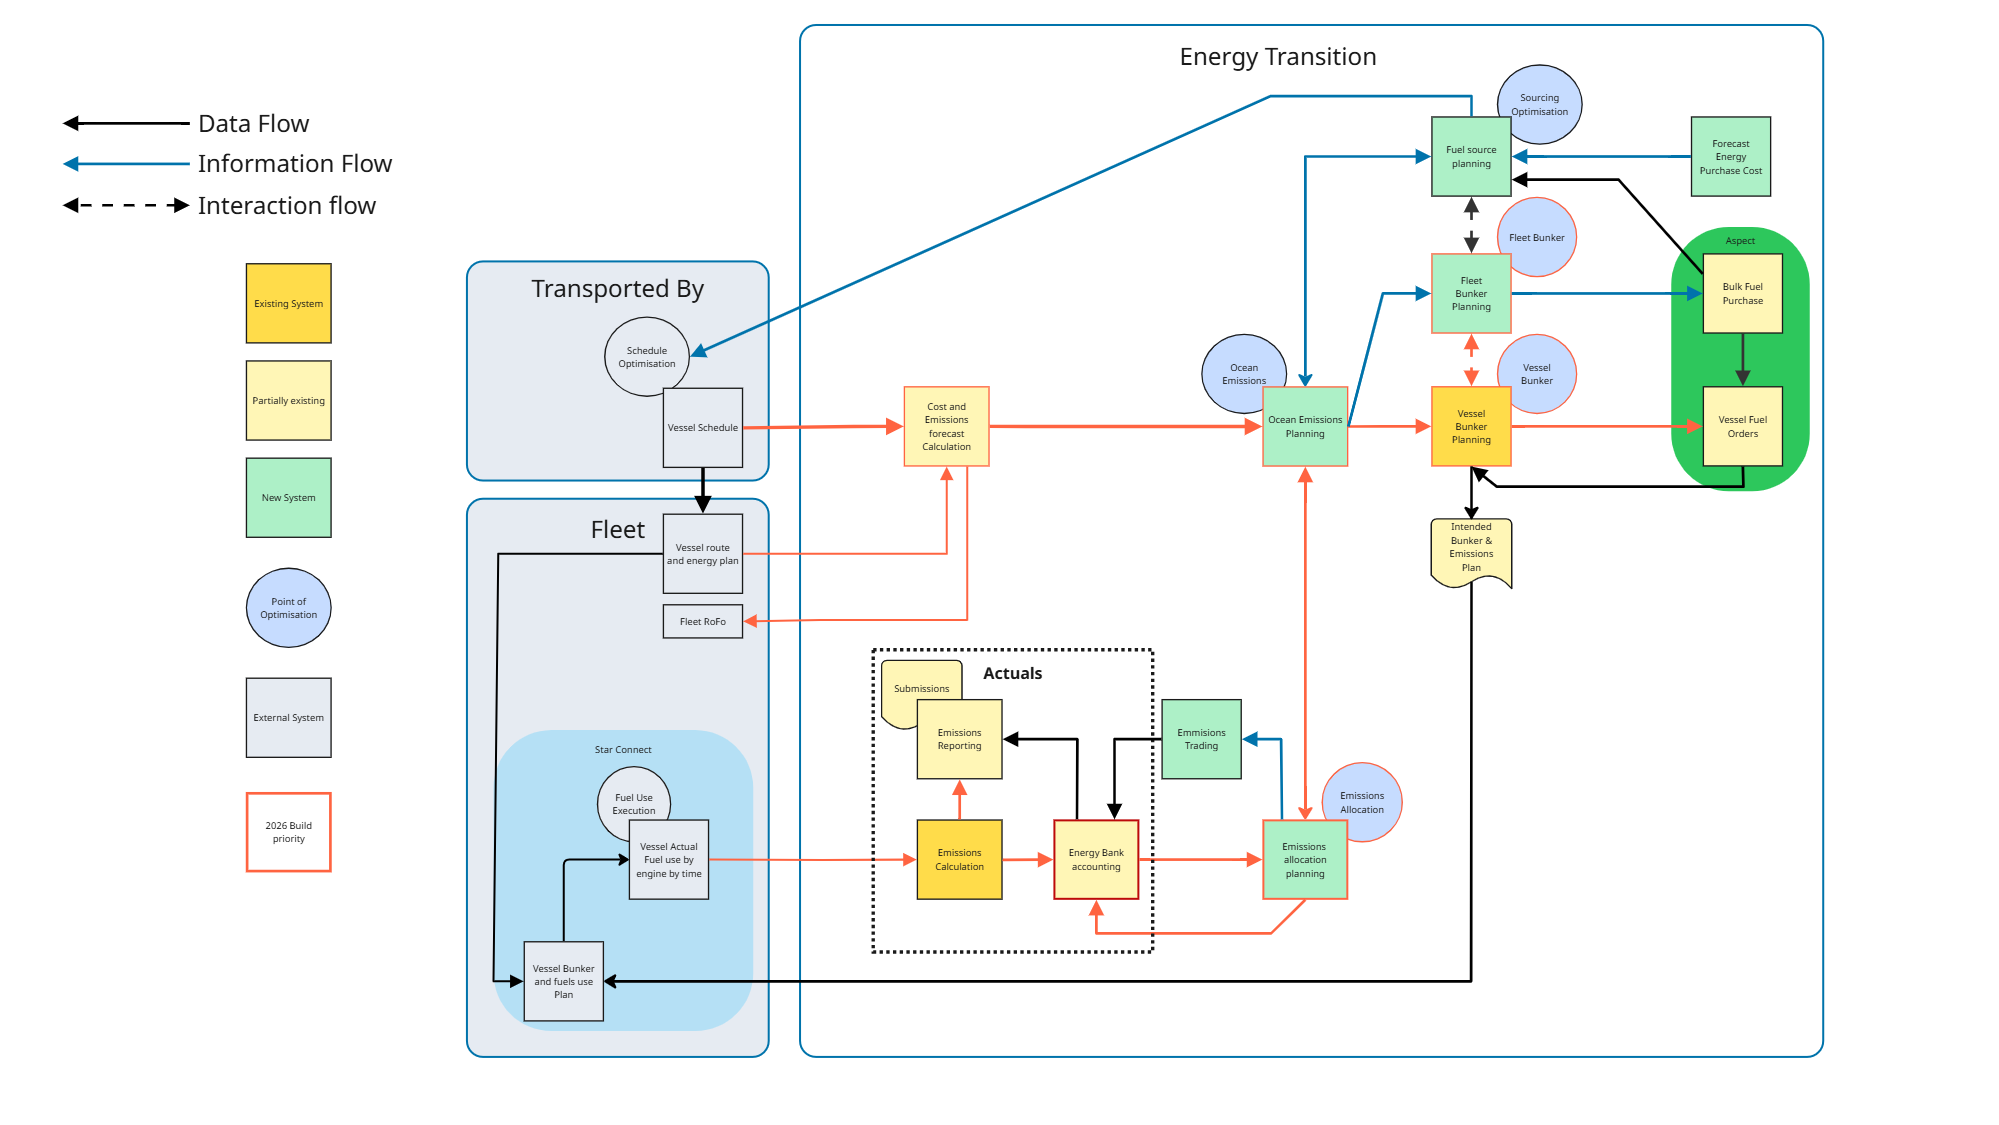
\includegraphics[width=\textwidth,keepaspectratio]{./system_overview_diagram.png}
\caption{Αρχιτεκτονική Συστήματος}
\end{figure}

Η λογική άποψη του συστήματος διακρίνει πέντε βασικά συστατικά
(\emph{components}): το \texttt{emissions\_workbench} ως κεντρικό domain
component, το \texttt{bunker/bow} και το \texttt{bunker/api} για τη
βελτιστοποίηση ανεφοδιασμού, καθώς και τα \texttt{ocean} και
\texttt{eco\_products} ως εξειδικευμένα, αυτόνομα components. Όλα
συνυπάρχουν σε ένα μονο-αποθετήριο (\emph{monorepo}) που διαχειρίζεται
την κοινή υποδομή, τη δοκιμή και την ανάπτυξη.

Η φυσική άποψη περιλαμβάνει δύο ανεξάρτητα deployment περιβάλλοντα
(παραγωγή και ενδιάμεσο περιβάλλον δοκιμής --- \emph{staging}), με τρία
αντίγραφα (\emph{replicas}) web server pod και ένα αποκλειστικό pod για
επεξεργασία παρασκηνίου (\emph{background processing}), όλα
ενορχηστρωμένα μέσω Azure Kubernetes Service. Η υψηλού επιπέδου ροή
δεδομένων ακολουθεί ένα μοτίβο αγωγού (\emph{pipeline}): εξωτερικές
πηγές (Dremio, Kafka, Shiptech) → στρώμα ενσωμάτωσης (\emph{ingestion
layer}) → domain logic → στρώμα παρουσίασης (LiveView) → αποθήκευση
αποτελεσμάτων (PostgreSQL, Azure Blob Storage).

Η ανάπτυξη ξεκίνησε το Μάρτιο του 2023 και το σύστημα μπήκε σε παραγωγή
τον Σεπτέμβριο του 2023 --- ένας κύκλος ανάπτυξης έξι μηνών από κενή
κατάσταση σε πλήρως λειτουργικό σύστημα παραγωγής. Η επιλογή της
αρχιτεκτονικής ήταν συνειδητά προσανατολισμένη στην ταχύτητα ανάπτυξης,
χωρίς να θυσιάζεται η επιχειρησιακή ορθότητα --- δεδομένου ότι τα
παραγόμενα δεδομένα χρησιμοποιούνται για κανονιστική συμμόρφωση (EU ETS,
CSRD) και εμπορικές συναλλαγές ύψους 31 εκατομμυρίων δολαρίων.

Αξίζει να σημειωθεί ότι η αρχιτεκτονική δεν σχεδιάστηκε εκ των προτέρων
ως ολοκληρωμένο blueprint, αλλά εξελίχθηκε σταδιακά υπό τις αρχές του
Extreme Programming (βλ. Κεφ. 10): απλούστατη δομή αρχικά, με συνεχή
ανακαινισμό (\emph{refactoring}) καθώς αποκαλύπτονταν νέες
επιχειρησιακές απαιτήσεις.

\section{9.2 Clean Architecture στην
πράξη}\label{clean-architecture-ux3c3ux3c4ux3b7ux3bd-ux3c0ux3c1ux3acux3beux3b7}

Η θεμελιώδης αρχιτεκτονική αρχή που διέπει τον κώδικα του NRG είναι η
\emph{Clean Architecture}, όπως αυτή τεκμηριώθηκε από τον Robert C.
Martin. Η αρχή αυτή οργανώνει τον κώδικα σε ομόκεντρα στρώματα με
αυστηρή κατευθυντήρια εξάρτηση: εξωτερικά στρώματα εξαρτώνται από
εσωτερικά, ενώ το αντίθετο απαγορεύεται.

Στο πλαίσιο του NRG, η αρχιτεκτονική αυτή υλοποιείται με τέσσερα
επίπεδα:

\textbf{Entities (Οντότητες):} Τα βασικά επιχειρησιακά δεδομένα και οι
κανόνες που θα υπήρχαν ακόμη και αν το σύστημα δεν ήταν
αυτοματοποιημένο. Στο NRG, αυτά περιλαμβάνουν έννοιες όπως
\texttt{ContainerMove}, \texttt{ClearingAccount}, \texttt{FuelOrder},
\texttt{Certificate} --- δομές δεδομένων χωρίς εξαρτήσεις σε εξωτερικά
frameworks.

\textbf{Use Cases (Περιπτώσεις Χρήσης):} Η επιχειρησιακή λογική της
εφαρμογής, ανεξάρτητη από web frameworks, βάσεις δεδομένων και λοιπές
υποδομές. Παράδειγμα: ο υπολογισμός εκπομπών ανά δρομολόγιο εμπεριέχει
την επιχειρησιακή λογική (\texttt{EmissionsCalculator}), αλλά δεν
γνωρίζει τίποτα για SQL ή HTTP. Τα use cases ορίζουν \emph{behaviours}
(συμπεριφορές) για τα δεδομένα που χρειάζονται, χωρίς να γνωρίζουν πώς
αυτά ανακτώνται.

\textbf{Adapters/Gateways (Προσαρμογείς):} Αποτελούν τη γέφυρα μεταξύ
των use cases και του εξωτερικού κόσμου. Τα \emph{Gateways} υλοποιούν
τις συμπεριφορές που ορίζουν τα use cases και αλληλεπιδρούν με εξωτερικά
συστήματα (PostgreSQL, Dremio, Kafka). Τα \emph{Web adapters} (LiveView,
HTTP controllers) εκχωρούν όλη την επεξεργασία δεδομένων στα use cases,
παρέχοντάς τους τα κατάλληλα Gateways.

\textbf{Frameworks/Drivers:} Το εξωτερικότερο στρώμα --- Phoenix, Ecto,
Kafka clients, Azure SDKs. Οι επιλογές αυτές μπορούν να αντικατασταθούν
χωρίς να επηρεαστεί η επιχειρησιακή λογική.

Ένα χαρακτηριστικό παράδειγμα εφαρμογής της Clean Architecture είναι το
σύστημα έκδοσης πιστοποιητικών (βλ. Κεφ. 6.5): το use case συγκεντρώνει
εκπομπές μέσω ενός gateway, υπολογίζει αποταμιεύσεις ανεξάρτητα από τη
βάση δεδομένων, και στη συνέχεια ο web controller μεριμνά για τη
μορφοποίηση και αποθήκευση του PDF --- κάθε στρώμα ξεχωριστό, με καθαρές
διεπαφές. Αυτή η αυστηρή διαστρωμάτωση επέτρεψε στην ομάδα να αλλάζει
τον τρόπο παραγωγής PDF χωρίς να αγγίξει τη λογική υπολογισμού εκπομπών.

Ένα ζήτημα που προκύπτει συχνά κατά την εφαρμογή Clean Architecture σε
Elixir είναι η σχέση με τις παραδοσιακές Phoenix conventions: το Phoenix
framework, από μόνο του, δεν επιβάλλει Clean Architecture --- απλοποιεί
την ανάπτυξη με controllers που απευθείας αλληλεπιδρούν με Ecto schemas.
Στο NRG, η ομάδα επέλεξε να υπερβεί αυτό το default pattern, εισάγοντας
ρητή Gateway layer: οι controllers και οι LiveView modules δεν
αλληλεπιδρούν ποτέ άμεσα με τους Ecto repos, αλλά μέσω Gateway modules
που υλοποιούν behaviours ορισμένα από τα use cases. Αυτή η επιλογή
αυξάνει ελαφρά το boilerplate, αλλά επιτρέπει πλήρη unit testing των use
cases χωρίς βάση δεδομένων --- κρίσιμο για τη διατήρηση του ρυθμού TDD
(βλ. Κεφ. 10).

Η Clean Architecture εκτός από τεχνική επιλογή αποτελεί και πολιτισμική
αρχή: η ομάδα χρησιμοποιεί τη διαστρωμάτωση ως κοινή γλώσσα στα code
reviews. Ερωτήματα του τύπου ``αυτό ανήκει στο use case ή στο gateway;''
αποτελούν τακτικές συζητήσεις στο pair programming (βλ. Κεφ. 10),
διαμορφώνοντας μια ομαδική κουλτούρα αρχιτεκτονικής συνέπειας ανεξάρτητα
από ατομικές προτιμήσεις.

\section{9.3 Monorepo
οργάνωση}\label{monorepo-ux3bfux3c1ux3b3ux3acux3bdux3c9ux3c3ux3b7}

Ολόκληρη η κωδικοβάση φιλοξενείται σε ένα ενιαίο αποθετήριο
(\emph{monorepo}) που συνδυάζει το εργαλείο \texttt{Workspace} για
ενορχήστρωση Elixir monorepo με Mix umbrella applications. Αυτή η
επιλογή αντανακλά μια συνειδητή αρχιτεκτονική απόφαση: η ατομική
διαχείριση πολλαπλών αποθετηρίων θα εισήγαγε σημαντική πολυπλοκότητα
συντονισμού σε μια κωδικοβάση όπου τα components μοιράζονται domain
γνώση και τεχνολογική υποδομή.

Τα πέντε κύρια components οργανώνονται κάτω από τον κατάλογο
\texttt{components/}:

\begin{itemize}
\tightlist
\item
  \texttt{emissions\_workbench}: Ο κεντρικός κόμβος --- Ocean Emissions,
  ECO Product Delivery, Energy Bank.
\item
  \texttt{bunker/bow}: Το web UI του συστήματος βελτιστοποίησης
  ανεφοδιασμού.
\item
  \texttt{bunker/api}: Ο coordinator service που επικοινωνεί με τον C++
  solver.
\item
  \texttt{ocean}: Αυτόνομο component για vessel master data και EU ETS
  δεδομένα.
\item
  \texttt{eco\_products} και \texttt{net\_zero}: Placeholder components
  για μελλοντική επέκταση.
\end{itemize}

Ένα κρίσιμο πλεονέκτημα του monorepo είναι η ανίχνευση επηρεαζόμενων
εφαρμογών (\emph{affected workspace apps}) κατά τη φάση CI/CD: αντί να
επανεκτελούνται τα tests για ολόκληρη την κωδικοβάση σε κάθε commit, το
σύστημα εντοπίζει ποια components επηρεάστηκαν από τις αλλαγές και
εκτελεί μόνο τα σχετικά tests --- αυτό επιτρέπει τη διατήρηση υψηλής
συχνότητας deployments (\textasciitilde32 ανά ημέρα) χωρίς αδικαιολόγητα
μεγάλους χρόνους αναμονής (βλ. Κεφ. 10 για CI/CD πρακτικές).

Ένα εγγενές μειονέκτημα είναι η αυξημένη πολυπλοκότητα κατασκευής
(\emph{build complexity}): η ατομική εκτέλεση ενός component απαιτεί
κατανόηση του γράφου εξαρτήσεων. Αυτό αντιμετωπίζεται μέσω τεκμηρίωσης
και εργαλείων ανίχνευσης εξαρτήσεων του \texttt{Workspace}.

Μια ενδιαφέρουσα πτυχή της monorepo οργάνωσης είναι ο τρόπος με τον
οποίο συνδυάζεται με το εργαλείο Nix: το \texttt{flake.nix} ορίζει ένα
ενιαίο, αναπαραγώγιμο development environment για ολόκληρο το
repository. Αυτό σημαίνει ότι ένας νέος developer που κλωνοποιεί το repo
εκτελεί μία μόνο εντολή (\texttt{nix\ develop}) και αποκτά ακριβώς την
ίδια έκδοση Elixir, Erlang, PostgreSQL, και όλων των βοηθητικών
εργαλείων που χρησιμοποιεί ολόκληρη η ομάδα --- ανεξάρτητα από το
λειτουργικό σύστημα ή τις τοπικές ρυθμίσεις.

\section{9.4 Components και τα όριά
τους}\label{components-ux3baux3b1ux3b9-ux3c4ux3b1-ux3ccux3c1ux3b9ux3ac-ux3c4ux3bfux3c5ux3c2}

Η οργάνωση σε components δεν είναι απλώς φυσική διαίρεση φακέλων ---
αντιπροσωπεύει σαφώς οριοθετημένα επιχειρησιακά contexts (βλ.
\emph{Domain-Driven Design}). Κάθε component εκθέτει μια δημόσια διεπαφή
και κρύβει τις εσωτερικές λεπτομέρειες υλοποίησης.

{\def\LTcaptype{} % do not increment counter
\begin{longtable}[]{@{}
  >{\raggedright\arraybackslash}p{(\linewidth - 4\tabcolsep) * \real{0.3548}}
  >{\raggedright\arraybackslash}p{(\linewidth - 4\tabcolsep) * \real{0.2258}}
  >{\raggedright\arraybackslash}p{(\linewidth - 4\tabcolsep) * \real{0.4194}}@{}}
\toprule\noalign{}
\begin{minipage}[b]{\linewidth}\raggedright
Component
\end{minipage} & \begin{minipage}[b]{\linewidth}\raggedright
Ρόλος
\end{minipage} & \begin{minipage}[b]{\linewidth}\raggedright
Δημόσια API
\end{minipage} \\
\midrule\noalign{}
\endhead
\bottomrule\noalign{}
\endlastfoot
\texttt{emissions\_workbench} & Κεντρικό domain: εκπομπές, ECO products,
Energy Bank & \texttt{Nrg.Ocean.*}, \texttt{EnergyBank.*},
\texttt{NrgWeb.*} \\
\texttt{bunker/bow} & Web UI βελτιστοποίησης ανεφοδιασμού & Phoenix
LiveView app, Oban workers \\
\texttt{bunker/api} & Coordinator για C++ solver & REST API, Port-based
IPC \\
\texttt{ocean} & Vessel master data + EU ETS &
\texttt{get\_all\_vessels/0}, \texttt{find\_by\_imo/1} \\
\texttt{eco\_products} & ECO product logic (placeholder) & Εξαρτάται από
emissions\_workbench \\
\end{longtable}
}

Η Elixir ως γλώσσα δεν διαθέτει access modifiers σε επίπεδο module,
επομένως τα όρια εφαρμόζονται κατά σύμβαση: δημόσιες συναρτήσεις στα
ανώτερα επίπεδα module path (πχ \texttt{EnergyBank.deposit/2}) αποτελούν
τη σύμβαση δημόσιας διεπαφής, ενώ modules με βαθύτερη ιεραρχία (πχ
\texttt{EnergyBank.Domain.Transactions.Withdrawal}) θεωρούνται
εσωτερικής χρήσης.

Τα όρια μεταξύ components επιβάλλονται επίσης μέσω της δομής εξαρτήσεων
στα Mix project files: ένα component δεν μπορεί να εισαγάγει κώδικα
άλλου component αν αυτή η εξάρτηση δεν είναι δηλωμένη ρητά. Αυτό
δημιουργεί ένα κατευθυνόμενο ακυκλικό γράφο (\emph{DAG}) εξαρτήσεων που
τεκμηριώνει τη συνολική αρχιτεκτονική δομή.

Εντός του \texttt{emissions\_workbench}, τα domain contexts οργανώνονται
επίσης ιεραρχικά: το \texttt{Nrg.Ocean} namespace ορίζει vessel master
data και emissions calculation, το \texttt{EnergyBank} namespace
διαχειρίζεται τη λογιστική καυσίμων, και το \texttt{NrgWeb} namespace
εκθέτει το web interface. Η επικοινωνία μεταξύ αυτών των contexts
γίνεται μέσω δημόσιων API συναρτήσεων, αποτρέποντας άμεση εξάρτηση
μεταξύ εσωτερικών modules. Αυτή η πρακτική, αν και δεν επιβάλλεται από
τον compiler, ελέγχεται στα code reviews ως αρχιτεκτονική αρχή της
ομάδας.

Ένα ζήτημα που αντιμετωπίζουν πολλά microservices architectures είναι η
διαχείριση δεδομένων που ανήκουν σε πολλαπλά contexts. Στο NRG, αυτό
αντιμετωπίζεται με ρητή αντιγραφή (\emph{copy-on-write}) μόνο των
απαραίτητων πεδίων: το \texttt{emissions\_workbench} αποθηκεύει τα
vessel data που χρειάζεται τοπικά, αντί να καλεί κάθε φορά το
\texttt{ocean} component. Αυτή η στρατηγική \emph{data sovereignty per
context} αυξάνει την τοπική συνοχή και μειώνει τη σύζευξη runtime, με το
κόστος πιθανής (διαχειρίσιμης) πλεονασματικής αποθήκευσης.

\section{9.5 Data ingestion pipeline}\label{data-ingestion-pipeline}

Ένας από τους αρχιτεκτονικά πιο ενδιαφέροντες τομείς του συστήματος
είναι ο τρόπος με τον οποίο δεδομένα από ετερογενείς εξωτερικές πηγές
εισέρχονται, κανονικοποιούνται και καθίστανται διαθέσιμα για
επεξεργασία. Η ενσωμάτωση δεδομένων (\emph{data ingestion})
αντιμετωπίζει τρεις διαφορετικές προκλήσεις: πηγές που απαιτούν
περιοδική ανάκτηση (\emph{polling}), ροές πραγματικού χρόνου
(\emph{streaming}) και σύνθετες εργασίες μετασχηματισμού (\emph{batch
processing}).

\subsection{9.5.1 Polling sources}\label{polling-sources}

Η ανάκτηση δεδομένων από το Dremio data lake και το Shiptech
πραγματοποιείται μέσω περιοδικής δειγματοληψίας που ενορχηστρώνεται από
Oban workers. Κάθε worker υλοποιεί ένα μοτίβο \emph{idempotent polling}:
διατηρεί ένα σελιδοδείκτη (\emph{bookmark}) \texttt{last\_updated} ώστε
να ανακτά μόνο τα νέα ή τροποποιημένα records, αποφεύγοντας
επαναλαμβανόμενη εισαγωγή.

Τα Dremio queries εκτελούνται μέσω ODBC, εκμεταλλευόμενα τον ODBC
adapter του Erlang OTP. Τα αποτελέσματα επιστρέφονται ως streaming
cursor, κατάλληλος για μεγάλα datasets χωρίς να φορτώνεται ολόκληρο το
result set στη μνήμη. Ο χρονοπρογραμματισμός ακολουθεί ημερήσιο κύκλο
για την πλειοψηφία των δεδομένων, με υψηλότερη συχνότητα για
time-sensitive streams (πχ vessel RoB).

Το Dremio λειτουργεί ως ενοποιητικό στρώμα δεδομένων (\emph{federated
data layer}) για το Maersk enterprise data ecosystem: αντί να αποθηκεύει
δεδομένα, δρομολογεί SQL queries σε υποκείμενα συστήματα (data
warehouses, data lakes, external databases). Για το NRG, αυτό σημαίνει
ότι τα δεδομένα εκπομπών ανά δρομολόγιο, τα trade factors και τα vessel
master data ανακτώνται μέσω ενιαίου SQL interface, ανεξάρτητα από το
υποκείμενο σύστημα αποθήκευσης. Η αρχιτεκτονική αντίσταση
(\emph{architectural insulation}) που παρέχει το Dremio επιτρέπει στο
NRG να παραμείνει αναλλοίωτο ακόμη και αν αλλάξει η υποκείμενη υποδομή
του enterprise data platform.

\subsection{9.5.2 Streaming}\label{streaming}

Η πραγματικού χρόνου ροή δεδομένων υλοποιείται μέσω Apache Kafka με την
Erlang βιβλιοθήκη \texttt{:brod}. Εννέα αρχεία ολοκλήρωσης Kafka
διαχειρίζονται topics που σχετίζονται με vessel telemetry (STAR Connect
feeds) και ocean emissions updates.

Η κατανομή των partitions ανά vessel αριθμό IMO εγγυάται διατήρηση της
σειράς μηνυμάτων ανά σκάφος --- προϋπόθεση σημαντική για σωστή
χρονολογική εφαρμογή των fuel consumption readings. Η διαχείριση offsets
επιτρέπει idempotent processing: αν ένας consumer αποτύχει και
επανεκκινηθεί, επεξεργάζεται εκ νέου τα μηνύματα από το τελευταίο
επιτυχώς δεσμευμένο offset.

Η επιλογή \texttt{:brod} (Erlang client για Kafka) αντί για pure Elixir
libraries (πχ \texttt{kafka\_ex}) αντικατοπτρίζει την αρχιτεκτονική
φιλοσοφία: η χρήση mature, low-level Erlang libraries παρέχει αξιοπιστία
και performance που δεν απαιτεί wrapper libraries. Το \texttt{:brod}
επιτρέπει fine-grained έλεγχο ανά partition consumer και υποστηρίζει
native Erlang process model για τη διαχείριση consumers.

Αξίζει να σημειωθεί η αρχιτεκτονική επιλογή για \emph{backpressure}: η
BEAM φυσικά περιορίζει το throughput μέσω message queue sizing. Αν ένας
downstream consumer δεν μπορεί να επεξεργαστεί μηνύματα αρκετά γρήγορα,
η BEAM mailbox γεμίζει και ο producer επιβραδύνεται φυσικά --- χωρίς
πολύπλοκο infrastructure για rate limiting. Αυτό απλοποιεί σημαντικά την
αρχιτεκτονική σε σχέση με JVM-based systems που απαιτούν ρητή διαχείριση
backpressure.

\subsection{9.5.3 Job processing και GenServer
Director}\label{job-processing-ux3baux3b1ux3b9-genserver-director}

Αφότου τα ακατέργαστα δεδομένα ενσωματωθούν, ακολουθεί ένας αγωγός
μετασχηματισμού: πρώτα αποθηκεύονται σε staging tables (πχ
\texttt{RawOceanContainerMove}), εμπλουτίζονται με αναφορικά δεδομένα
(vessel data, trade factors, emissions factors) και τελικά μεταφέρονται
στους κύριους πίνακες.

Η διαχείριση των background workers υλοποιείται μέσω του
\texttt{NrgWorker.Director}, ενός GenServer που παρακολουθεί αλλαγές
διαμόρφωσης και εκκινεί ή τερματίζει workers δυναμικά:

\begin{verbatim}
defmodule NrgWorker.Director do
  @moduledoc "Listens for worker config changes and starts/stops workers accordingly."

  use GenServer

  @spec start_link(keyword()) :: GenServer.on_start()
  def start_link(init_args \\ []) do
    GenServer.start_link(__MODULE__, init_args, name: __MODULE__)
  end

  @impl GenServer
  def init(_opts) do
    NrgWorker.Settings.subscribe(:worker_config)
    {:ok, [], {:continue, :apply_current_worker_config}}
  end

  @impl GenServer
  def handle_continue(:apply_current_worker_config, state) do
    NrgWorker.Settings.latest_worker_config() |> apply_config()
    {:noreply, state}
  end

  @impl GenServer
  def handle_info({:worker_config, :changed}, state) do
    NrgWorker.Settings.latest_worker_config() |> apply_config()
    {:noreply, state}
  end

  # Starts and stops workers based on the contents of `new_config`
  @spec apply_config(map()) :: :ok
  defp apply_config(new_config) do
    Enum.each(new_config, fn {field, should_be_running?} ->
      if field in NrgWorker.worker_config_fields() do
        worker = NrgWorker.find_by_config_field(field)

        if should_be_running?,
          do: NrgWorker.start(worker, NrgWorker.Supervisor),
          else: NrgWorker.stop(worker)
      end
    end)

    :ok
  end
end
\end{verbatim}

\textbf{Λήμμα 9.5.1:} \texttt{NrgWorker.Director} GenServer --- δυναμική
διαχείριση workers μέσω subscription σε αλλαγές διαμόρφωσης.

Η αρχιτεκτονική αυτή επιτρέπει run-time ενεργοποίηση ή απενεργοποίηση
κάθε worker χωρίς επανεκκίνηση της εφαρμογής --- κρίσιμο για λειτουργική
ευελιξία σε production περιβάλλον. Ο Director εγγράφεται
(\texttt{subscribe}) σε αλλαγές ρυθμίσεων και αντιδρά άμεσα,
ακολουθώντας το BEAM μοτίβο της επικοινωνίας μέσω μηνυμάτων. Η χρήση
\texttt{\{:continue,\ :apply\_current\_worker\_config\}} στο
\texttt{init/1} εξασφαλίζει ότι η αρχική διαμόρφωση εφαρμόζεται αμέσως
μετά την εκκίνηση, χωρίς να μπλοκαριστεί ο supervisor.

\section{9.6 Web layer}\label{web-layer}

Το στρώμα παρουσίασης βασίζεται αποκλειστικά σε Phoenix LiveView,
επιτρέποντας διαδραστικές, server-rendered εμπειρίες χρήστη χωρίς
client-side JavaScript framework.

\begin{itemize}
\tightlist
\item
  \textbf{Eco Delivery}: Παρακολούθηση ECO product allocations, έκδοση
  πιστοποιητικών, dashboard επισκόπησης.
\item
  \textbf{Energy Bank}: Διαχείριση clearing accounts, προβολή
  καταθέσεων/αναλήψεων, ισοζύγιο καυσίμων.
\item
  \textbf{Emissions Data Inventory}: Αναζήτηση εκπομπών ανά πελάτη,
  export δεδομένων, ιστορικά reports.
\item
  \textbf{Admin}: Διαχείριση ρυθμίσεων συστήματος, worker configuration,
  user roles.
\end{itemize}

Τα LiveView modules ακολουθούν το Humble Object pattern: η παρουσίαση
(mount/handle\_event/render) διαχωρίζεται από την επιχειρησιακή λογική,
την οποία εκχωρούν σε use case modules. Αυτό επιτρέπει αποτελεσματική
δοκιμή της επιχειρησιακής λογικής ανεξάρτητα από το web layer (βλ. Κεφ.
10 για TDD πρακτικές).

Η ενσωμάτωση με το Maersk Design System (MDS) --- μια βιβλιοθήκη Web
Components --- εξασφαλίζει οπτική συνέπεια με άλλες εφαρμογές του
ομίλου. Τα MDS components χρησιμοποιούνται ως custom HTML elements εντός
των Phoenix HEEx templates, διατηρώντας τη διαχωριστική γραμμή μεταξύ
περιεχομένου (Elixir) και παρουσίασης (MDS). Τα static assets
διαχειρίζονται από \texttt{esbuild} με Phoenix integration.

Η επικοινωνία μεταξύ sessions χρηστών για πραγματικού χρόνου ενημερώσεις
χρησιμοποιεί το Phoenix PubSub: όταν ένας worker ολοκληρώνει μια
εισαγωγή δεδομένων, ενημερώνει τα ενεργά LiveView sessions μέσω
broadcast, ώστε οι χρήστες να βλέπουν ενημερωμένα δεδομένα χωρίς manual
refresh.

Η αρχιτεκτονική επιλογή Phoenix LiveView αντί για SPA (Single Page
Application) με React ή Vue έχει συγκεκριμένες επιπτώσεις στη δομή του
κώδικα: ολόκληρη η λογική κατάστασης (\emph{state management}) παραμένει
στον server, εξαλείφοντας την ανάγκη για client-state synchronization. Ο
server αποστέλλει ελάχιστα diffs HTML μέσω WebSocket αντί για JSON
payloads, μειώνοντας τη σύζευξη client-server. Το κόστος αυτής της
επιλογής είναι η υψηλότερη εξάρτηση από WebSocket connectivity ---
αποδεκτό κόστος για εταιρικούς χρήστες σε αξιόπιστα δίκτυα.

Επιπλέον, η χρήση LiveComponents για επαναχρησιμοποιήσιμα UI elements
(πχ emissions summary cards, certificate status badges) εφαρμόζει την
αρχή DRY εντός του web layer, μειώνοντας duplicated template logic. Κάθε
LiveComponent διαχειρίζεται ανεξάρτητα την κατάστασή του, επιτρέποντας
partial re-renders χωρίς να ανανεώνεται ολόκληρη η σελίδα.

\section{9.7 Authentication και
Authorization}\label{authentication-ux3baux3b1ux3b9-authorization}

Η ταυτοποίηση χρηστών βασίζεται σε SAML SSO μέσω Azure Active Directory.
Κάθε χρήστης αυθεντικοποιείται μέσω του εταιρικού identity provider της
Maersk, ενώ οι πληροφορίες ταυτότητας και ρόλων προέρχονται από AD
groups.

Η εξουσιοδότηση (\emph{authorization}) υλοποιείται με ρόλους βασισμένους
σε ομάδες Azure AD. Ομάδες όπως ``SBTi Developers'' ή ``ECO Sales''
αντιστοιχίζονται σε internal ρόλους της εφαρμογής. Στα LiveView mounts,
ο έλεγχος ρόλων πραγματοποιείται με helper macros τύπου
\texttt{with\_authenticated\_request(ctx,\ roles:\ \textasciitilde{}ROLES(admin))},
παρέχοντας διαδηλωτικό (\emph{declarative}) και επαναχρησιμοποιήσιμο
έλεγχο πρόσβασης.

Για πρόσβαση σε production περιβάλλον, χρησιμοποιείται Privileged
Identity Management (PIM) της Azure --- ένα σύστημα just-in-time
πρόσβασης όπου ο χρήστης αιτείται ανύψωση προνομίων για συγκεκριμένο
χρονικό διάστημα. Αυτό ελαχιστοποιεί την επιφάνεια επίθεσης σε περίπτωση
παραβίασης λογαριασμού, και δημιουργεί ακριβές audit trail κάθε
πρόσβασης στα production συστήματα --- απαίτηση που προέκυψε άμεσα από
τον εσωτερικό έλεγχο GIA του 2023 (βλ. Κεφ. 2.7).

Τα secrets της εφαρμογής (credentials βάσεων δεδομένων, API keys)
διαχειρίζονται μέσω HashiCorp Vault, με AppRole authentication για τα
CI/CD pipelines. Ο διαχωρισμός μεταξύ runtime secrets (Vault) και
build-time secrets (agenix) αντικατοπτρίζει την αρχιτεκτονική αρχή της
ελάχιστης δυνατής έκθεσης κατά την κάθε φάση.

Αξιοσημείωτη αρχιτεκτονική λεπτομέρεια είναι η απουσία session-level
authorization state: κάθε LiveView request επαληθεύει τη συνεδρία
(\emph{session}) και τα δικαιώματα ανεξάρτητα, αντί να εκχωρεί αποφάσεις
authorization σε cached state. Αυτό προστατεύει από κατηγορία επιθέσεων
όπου η ανάκληση δικαιωμάτων (πχ αποχώρηση χρήστη) δεν αντανακλάται άμεσα
σε ενεργές sessions. Στο πλαίσιο του NRG, όπου οι χρήστες έχουν πρόσβαση
σε εμπιστευτικά οικονομικά δεδομένα πελατών, αυτή η προσέγγιση αποτελεί
ορθή αρχιτεκτονική επιλογή.

\section{9.8 Persistence layer}\label{persistence-layer}

Η κεντρική αποθήκευση δεδομένων του συστήματος βασίζεται σε PostgreSQL
Flexible Server στο Azure.

Η κρίσιμη αρχιτεκτονική απόφαση αφορά τη χρήση \textbf{πολλαπλών βάσεων
δεδομένων} αντί ενός ενιαίου αποθετηρίου: κάθε domain context έχει δική
του Ecto Repo. Αυτό επιτρέπει:

\begin{itemize}
\tightlist
\item
  \textbf{Απομόνωση σφαλμάτων} (\emph{blast radius}): πρόβλημα στη βάση
  δεδομένων του Energy Bank δεν επηρεάζει άμεσα τις Ocean emissions.
\item
  \textbf{Ανεξάρτητη κλιμάκωση}: κάθε βάση μπορεί να διαμορφωθεί
  ανεξάρτητα (storage, compute, backup policy).
\item
  \textbf{Καθαρά domain boundaries}: η αδυναμία foreign key constraints
  μεταξύ βάσεων αναγκάζει explicit modeling των cross-context
  relationships στον κώδικα.
\end{itemize}

Η στρατηγική δημιουργίας αντιγράφων ασφαλείας (\emph{backup strategy})
αξιοποιεί το Azure Data Protection με ημερήσιες και εβδομαδιαίες λήψεις
αντιγράφων. Κρίσιμο στοιχείο είναι τα αυτοματοποιημένα εβδομαδιαία τεστ
αποκατάστασης: ένα GitHub Actions workflow
(\texttt{db-restore-from-backup.yml}) εκτελείται κάθε Παρασκευή,
αποκαθιστά τη βάση δεδομένων σε δοκιμαστικό περιβάλλον και επαληθεύει
την ακεραιότητα των δεδομένων. Αυτή η πρακτική, σπάνια σε πολλές
οργανώσεις, εξασφαλίζει ότι το RTO (Recovery Time Objective) παραμένει
μετρήσιμο και επαληθευμένο, και όχι θεωρητικό.

Οι migrations ακολουθούν αρχή αντίστροφης συμβατότητας
(\emph{backward-compatible migrations only}): κάθε αλλαγή σχήματος
πρέπει να είναι συμβατή με την προηγούμενη έκδοση κώδικα, επιτρέποντας
zero-downtime deployments με κυλιόμενη ενημέρωση pods.

Η χρήση Ecto ως ORM (αντικειμενο-σχεσιακός χαρτογράφος ---
\emph{Object-Relational Mapper}) παρέχει τυπική ασφάλεια για queries
μέσω Ecto.Query DSL, ενώ τα Changesets εγγυώνται επικύρωση δεδομένων
πριν από κάθε εγγραφή.

\section{9.9 Event sourcing για Energy
Bank}\label{event-sourcing-ux3b3ux3b9ux3b1-energy-bank}

Το υποσύστημα Energy Bank αποτελεί αρχιτεκτονικά το πιο σύνθετο τμήμα
του συστήματος, επιλέγοντας το μοτίβο \emph{Event Sourcing} σε συνδυασμό
με \emph{CQRS (Command Query Responsibility Segregation)}. Η επιλογή
αυτή δεν είναι τυχαία: το πρόβλημα της λογιστικής καυσίμων απαιτεί
πλήρες ελεγκτικό ίχνος (\emph{audit trail}), δυνατότητα αναπαραγωγής
(\emph{event replay}) για επαναϋπολογισμό ισοζυγίων, και αμεταβλητότητα
του ιστορικού --- ιδιότητες που το event sourcing παρέχει φυσικά.

Η αρχιτεκτονική ακολουθεί το μοτίβο Commands → Aggregates → Events →
Projections, υλοποιούμενο με τη βιβλιοθήκη \texttt{Commanded} και
EventStore backend (αποθήκευση event stream σε PostgreSQL).

Η δομή λειτουργεί ως εξής: ένα \textbf{Command} εκφράζει πρόθεση (πχ
``ανάληψη ποσότητας ενέργειας''), επικυρώνεται και διαβιβάζεται στο
αντίστοιχο \textbf{Aggregate} (\texttt{ClearingAccount}). Το Aggregate
εφαρμόζει τους επιχειρησιακούς κανόνες (πχ ο λογαριασμός πρέπει να έχει
επαρκές υπόλοιπο), και αν η επικύρωση επιτύχει, παράγει ένα
\textbf{Event} (\texttt{EnergyWithdrawn}) που αποθηκεύεται αμετάβλητα
στο EventStore. Τα Events τροφοδοτούν \textbf{Projections} --- read
models που υπολογίζουν τρέχουσα κατάσταση (πχ τρέχον υπόλοιπο clearing
account).

Το παρακάτω λήμμα παρουσιάζει το Command και τον CommandHandler για
ανάληψη ενέργειας:

\begin{verbatim}
defmodule EnergyBank.Application.Transactions.WithdrawEnergy do
  defmodule Command do
    use Ecto.Schema
    import Ecto.Changeset

    @fields [
      :transaction_id,
      :account_id,
      :amount,
      :withdrawn_at,
      :recorded_at
    ]

    @primary_key false
    embedded_schema do
      field :transaction_id, :string
      field :account_id, :string
      field :amount, :decimal
      field :withdrawn_at, :naive_datetime
      field :recorded_at, :naive_datetime
    end

    def new!(attrs) do
      %__MODULE__{}
      |> cast(attrs, @fields)
      |> validate_required(@fields)
      |> apply_action!(:new)
    end
  end

  defmodule CommandHandler do
    alias EnergyBank.Domain.Transactions.Withdrawal

    @behaviour Commanded.Commands.Handler

    @impl Commanded.Commands.Handler
    def handle(state, %Command{} = command) do
      Withdrawal.withdraw(state, command |> Map.from_struct())
    end
  end
end
\end{verbatim}

\textbf{Λήμμα 9.9.1:}
\texttt{EnergyBank.Application.Transactions.WithdrawEnergy} --- Command
και CommandHandler για ανάληψη ενέργειας από clearing account.

Αξίζει να σημειωθεί η διαχωριστική γραμμή ευθύνης: το \texttt{Command}
module χρησιμοποιεί Ecto για επικύρωση εισόδου (cast,
validate\_required), ενώ το \texttt{CommandHandler} αναθέτει την
επιχειρησιακή λογική αποκλειστικά στο \texttt{Withdrawal.withdraw/2}
domain module. Ο CommandHandler δεν γνωρίζει τίποτα για βάσεις δεδομένων
--- εφαρμόζει Clean Architecture στο επίπεδο event sourcing.

Ένα ιδιαίτερο χαρακτηριστικό του event sourcing είναι η δυνατότητα
\emph{re-projection}: σε περίπτωση αλλαγής επιχειρησιακής λογικής (πχ
νέος τρόπος υπολογισμού ισοζυγίου), το σύστημα μπορεί να επαναλάβει
ολόκληρο το history των events και να δημιουργήσει εκ νέου τις
projections. Αυτό παρέχει ασυνήθιστη ευελιξία για επιχειρησιακά
συστήματα που εξελίσσονται παράλληλα με ρυθμιστικές αλλαγές (βλ. Κεφ.
6.3 για επιχειρησιακή περιγραφή).

Μια σημαντική αρχιτεκτονική πτυχή είναι η διαχείριση \emph{eventual
consistency} μεταξύ commands και projections: όταν ένα command
ολοκληρώνεται επιτυχώς, το αντίστοιχο event εγγράφεται στο EventStore,
αλλά η projection ενδέχεται να μην έχει ακόμη ενημερωθεί. Σε scenarios
όπου το UI πρέπει να εμφανίσει αμέσως το αποτέλεσμα μιας ενέργειας,
απαιτείται μηχανισμός \texttt{wait\_until} που αναμένει την ενημέρωση
της projection. Αυτό αποτελεί ένα από τα πιο λεπτά θέματα σχεδίασης σε
event-sourced συστήματα, και η ομάδα το αντιμετωπίζει με ρητή επιλογή
ανά feature: τα περισσότερα UI flows αποδέχονται ελάχιστη καθυστέρηση,
ενώ κρίσιμες λειτουργίες (πχ επαλήθευση υπολοίπου πριν withdrawal)
χρησιμοποιούν σύγχρονη επαλήθευση.

Ο συνδυασμός CQRS με event sourcing επιτρέπει επίσης ανεξάρτητη
βελτιστοποίηση read/write paths: τα command paths βελτιστοποιούνται για
consistency και atomic writes, ενώ τα query paths (projections)
βελτιστοποιούνται για ταχύτητα ανάγνωσης. Για την Energy Bank, αυτό
σημαίνει ότι τα reports υπολοίπου clearing accounts ανακτώνται από
pre-computed read models, ενώ νέες καταθέσεις/αναλήψεις γράφουν
αποκλειστικά στο event stream.

\section{9.10 Observability
αρχιτεκτονική}\label{observability-ux3b1ux3c1ux3c7ux3b9ux3c4ux3b5ux3baux3c4ux3bfux3bdux3b9ux3baux3ae}

Η παρατηρησιμότητα (\emph{observability}) αντιμετωπίζεται αρχιτεκτονικά,
όχι ως εκ των υστέρων προσθήκη. Τα τρία επίπεδα --- logs, metrics,
traces --- ενσωματώνονται σε κάθε στρώμα του συστήματος, από το Phoenix
request lifecycle ως τους Oban workers και τους Kafka consumers.

\begin{itemize}
\tightlist
\item
  \textbf{Logs} συλλέγονται μέσω Grafana Loki με LogQL για structured
  querying.
\item
  \textbf{Metrics} ρέουν μέσω PromEx (βιβλιοθήκη Elixir για Prometheus)
  → Prometheus → Grafana dashboards.
\item
  \textbf{Traces} προωθούνται μέσω OpenTelemetry σε OpenObserve
  (self-hosted instance, v0.14.4), με propagation context που διατρέχει
  HTTP requests, BEAM processes, database queries και Kafka messages.
  Αυτό επιτρέπει ανίχνευση μιας αίτησης από το LiveView mount ως τις
  εγγραφές βάσης δεδομένων.
\end{itemize}

Η στρατηγική alerting υλοποιείται ως κώδικας (\emph{alerts-as-code}) σε
YAML. Οι κανόνες ειδοποίησης ομαδοποιούνται σύμφωνα με διαφορετικά
επίπεδα κρισιμότητας και χρονικούς ορίζοντες.

Ένας χαρακτηριστικός κανόνας ειδοποίησης που αφορά την ακεραιότητα των
δεδομένων:

\begin{verbatim}
- name: NRG Energy Transition alerts
  interval: 1m
  rules:
    - alert: Too many concurrent requests to ETW
      expr: sum(nrg_etw_requests_count{app="nrg-workers"}) by(env) > 5
      for: 5m0s
      labels:
        hedwig_scope: nrg-errors-scope
      annotations:
        runbook_url: https://maersk-tools.atlassian.net/wiki/x/lIl0iio
        summary: Too many current requests to ETW
        description: We've made too many concurrent requests to ETW in an environment.
\end{verbatim}

\textbf{Λήμμα 9.10.1:} Alert rule για ανίχνευση υπερβολικής παράλληλης
φόρτωσης των External Trade Workbench (ETW) workers.

Ο κανόνας αυτός αξιολογείται κάθε λεπτό και ενεργοποιείται αν
εντοπιστούν περισσότερα από 5 ταυτόχρονα requests στο ETW για διάστημα 5
λεπτών. Η ετικέτα \texttt{hedwig\_scope:\ nrg-errors-scope} δρομολογεί
την ειδοποίηση μέσω Hedwig --- εσωτερικό σύστημα ειδοποίησης της Maersk
--- σε κανάλια Teams και email.

Πέρα από τα τεχνικά alerts (CrashLoopBackOff, cluster unreachability,
non-200 spike), το σύστημα παρακολουθεί \textbf{επιχειρησιακές
μετρικές}:

\begin{itemize}
\tightlist
\item
  Ο Ingestion Worker δεν έχει αναφέρει θετικό count εισαγωγής εντός 72
  ωρών.
\item
  Ο Enrichment Worker δεν έχει ολοκληρώσει εργασία εντός 6 ωρών.
\item
  Δεδομένα πλοίων (\emph{Vessel Voyage data}) πιο παλαιά από 49 ώρες.
\item
  Ανεκχώρητες εκπομπές (\emph{unallocated emissions}) άνω του 2\%.
\item
  Αποτυχία Energy Bank Projector.
\end{itemize}

Αυτή η πρακτική --- ορισμός ορίων \emph{freshness} για business-critical
δεδομένα --- αντανακλά την επιχειρησιακή ωριμότητα του συστήματος. Η
ανίχνευση ενός stale ingestion worker δεν αποτελεί απλώς τεχνικό alert,
αλλά σηματοδοτεί πιθανή επίπτωση στην εγκυρότητα υπολογισμών εκπομπών
--- εγκυρότητα που κρίνεται από regulators και εξωτερικούς ελεγκτές.

Οι ειδοποιήσεις συνοδεύονται πάντα από \emph{runbook URLs}, παρέχοντας
στον on-call engineer βήμα-βήμα οδηγίες αποκατάστασης.

Η αρχιτεκτονική telemetry ακολουθεί το Elixir \texttt{Telemetry} library
pattern: κάθε σημαντικό σημείο του συστήματος εκπέμπει named events (πχ
\texttt{{[}:nrg,\ :ocean,\ :emissions\_calculation,\ :stop{]}}) με
μετρήσεις και metadata. Το PromEx library συνδέεται αυτόματα σε Phoenix,
Ecto και Oban telemetry events, δημιουργώντας Prometheus metrics χωρίς
χειροκίνητο instrumentation. Για custom business metrics (πχ
\texttt{nrg\_etw\_requests\_count},
\texttt{nrg\_worker\_ingestion\_sum}), η ομάδα ορίζει ρητά telemetry
events στα κατάλληλα σημεία του κώδικα.

Το distributed tracing μέσω OpenTelemetry παρέχει ένα πλήρες trace για
κάθε user request: από το LiveView event handler, μέσω use cases και
gateways, ως τα SQL queries και τα Kafka messages. Αυτό επιτρέπει
διάγνωση performance bottlenecks που δεν εντοπίζονται από metrics μόνο
--- πχ αν ένα συγκεκριμένο query αργεί μόνο για συγκεκριμένους πελάτες
με μεγάλο αριθμό container moves. Η αρχιτεκτονική παρατηρησιμότητας
συνδέεται άμεσα με τις τεχνολογικές επιλογές που αναλύονται στο Κεφ. 8.

\section{9.11 Deployment topology}\label{deployment-topology}

Η τοπολογία ανάπτυξης αντικατοπτρίζει τις αρχές της διαθεσιμότητας, της
κλιμάκωσης και της απλότητας λειτουργίας.

\textbf{Εισερχόμενος traffic} ακολουθεί την αλυσίδα: Akamai CDN →
Stargate (εσωτερικό API gateway Maersk) → Azure Kubernetes Service
ingress controller → Kubernetes pods. Το Akamai παρέχει DDoS προστασία
και global routing, ενώ το Stargate επιβάλλει εταιρικές πολιτικές
ασφαλείας και rate limiting.

\textbf{Kubernetes pods} οργανώνονται σε δύο τύπους:

\begin{itemize}
\tightlist
\item
  \textbf{3 web server replicas}: εξυπηρέτηση HTTP/WebSocket traffic,
  Phoenix LiveView connections, certificate downloads.
\item
  \textbf{1 worker pod}: background processing --- Oban jobs, Kafka
  consumers, Nrg Worker processes που διαχειρίζεται ο Director.
\end{itemize}

Ο διαχωρισμός web/worker επιτρέπει ανεξάρτητη κλιμάκωση: αν ο αριθμός
των background workers χρειαστεί αύξηση, αλλάζει ο αριθμός replicas του
worker pod χωρίς να επηρεαστεί ο web layer.

\textbf{Rolling deployments} αποτελούν τον τρόπο ενημέρωσης: το
Kubernetes αντικαθιστά σταδιακά τα pods ένα-ένα, εξασφαλίζοντας ότι
κάποιες replicas παραμένουν διαθέσιμες καθ' όλη τη διάρκεια. Αυτό, σε
συνδυασμό με backward-compatible migrations (βλ. 9.8), επιτρέπει
zero-downtime deployments --- σημαντικό για ένα σύστημα με 1.300
ενεργούς χρήστες.

Η ανάπτυξη εκτελείται μέσω ενός custom \texttt{k8s} binary, wrapper πάνω
σε \texttt{kubectl} κατασκευασμένο με Nix, που ενσωματώνει εταιρικές
πρακτικές ανάπτυξης. Τα GitHub Actions workflows αυτοματοποιούν τον
κύκλο build → test → deploy (βλ. Κεφ. 8 για CI/CD τεχνολογίες).

Το σύστημα λειτουργεί σε δύο ανεξάρτητα περιβάλλοντα: \emph{staging} για
επαλήθευση πριν την παραγωγή, και \emph{production} για τους τελικούς
χρήστες. Η δομή infrastructure-as-code (Terraform) εξασφαλίζει ότι και
τα δύο περιβάλλοντα είναι ισοδύναμα, αποτρέποντας το ``works on staging,
fails in production'' σύνδρομο.

Η ροή ανάπτυξης ακολουθεί trunk-based development: ο κώδικας
συγχωνεύεται στο \texttt{main} branch, το CI pipeline επικυρώνει (build,
test, security scan), και στη συνέχεια γίνεται αυτόματο deploy στο
staging, ακολουθούμενο --- μετά από επιβεβαίωση --- από deploy στο
production. Η διαδικασία είναι ελαφριά και αυτοματοποιημένη, με ελάχιστη
χειροκίνητη παρέμβαση. Αυτή η υψηλή συχνότητα deployments ---
χαρακτηριστική των XP πρακτικών (βλ. Κεφ. 10) --- απαιτεί ισχυρή
αυτοματοποίηση, αξιόπιστα test suites και backward-compatible
migrations, τρεις αρχιτεκτονικές ιδιότητες που αποτελούν προτεραιότητα.

\section{9.12 Disaster recovery και
αναπαραγωγιμότητα}\label{disaster-recovery-ux3baux3b1ux3b9-ux3b1ux3bdux3b1ux3c0ux3b1ux3c1ux3b1ux3b3ux3c9ux3b3ux3b9ux3bcux3ccux3c4ux3b7ux3c4ux3b1}

Η αρχιτεκτονική αναπαραγωγιμότητας του NRG βασίζεται σε τρεις
αλληλοσυμπληρούμενες αρχές: υποδομή ως κώδικας, αναπαραγώγιμες
κατασκευές (\emph{reproducible builds}) και δοκιμασμένη αποκατάσταση.

\textbf{Υποδομή ως κώδικας μέσω Terraform:} Ολόκληρη η υποδομή Azure
(databases, AKS cluster, storage accounts, networking) ορίζεται σε
αρχεία \texttt{.tf}. Σε περίπτωση καταστροφικής αποτυχίας, η υποδομή
μπορεί να ανοικοδομηθεί από μηδενική βάση εκτελώντας
\texttt{terraform\ apply}.

\textbf{Αναπαραγώγιμες κατασκευές μέσω Nix:} Το \texttt{flake.nix}
ορίζει κλειδωμένες (\emph{locked}) εξαρτήσεις για όλα τα εργαλεία
ανάπτυξης, εξασφαλίζοντας ότι κάθε μέλος της ομάδας και κάθε CI runner
χρησιμοποιεί ακριβώς την ίδια έκδοση εργαλείων. Αυτό εξαλείφει μια
ολόκληρη κατηγορία σφαλμάτων (``it works on my machine'') και απλοποιεί
σημαντικά το onboarding νέων μελών.

\textbf{Δοκιμασμένη αποκατάσταση βάσης δεδομένων:} Εβδομαδιαία
αυτοματοποιημένη επαλήθευση αντιγράφων ασφαλείας μέσω του workflow
\texttt{db-restore-from-backup.yml}. Η αποκατάσταση χρησιμοποιεί
\emph{Point-In-Time Recovery (PITR)} της Azure, επιτρέποντας επαναφορά
της βάσης σε οποιοδήποτε χρονικό σημείο εντός του παραθύρου διατήρησης.

Τα ενδεικτικά μεγέθη αποκατάστασης εκτιμώνται ως εξής:

\begin{itemize}
\tightlist
\item
  \textbf{RTO (Recovery Time Objective):} Υποδομή \textasciitilde2 ώρες
  (Terraform apply), εφαρμογή \textasciitilde30 λεπτά (Kubernetes
  deploy), βάση δεδομένων από PITR \textasciitilde1 ώρα.
\item
  \textbf{RPO (Recovery Point Objective):} Ελάχιστη απώλεια δεδομένων
  λόγω PITR και continuous backups.
\end{itemize}

Σε σενάρια μερικής αποτυχίας (πχ αποτυχία ενός pod), το Kubernetes
αντιμετωπίζει αυτόματα την κατάσταση μέσω health checks και
αντικατάσταση pods. Τα \texttt{CrashLoopBackOff} alerts (30 δευτερόλεπτα
interval) εξασφαλίζουν ότι η ομάδα ειδοποιείται άμεσα για
επανεκκινούμενα pods, ενώ τα runbooks παρέχουν δομημένη διαδικασία
διερεύνησης και αποκατάστασης.

Η συνολική αρχιτεκτονική αναπαραγωγιμότητας υπηρετεί και σκοπούς
ελέγχου: ο εσωτερικός έλεγχος GIA του 2023 (βλ. Κεφ. 2.7) έθεσε ρητά
απαιτήσεις για \emph{audit trail}, \emph{data tracking} και
\emph{reproducibility}. Το συνδυασμένο χαρτοφυλάκιο event sourcing
(Energy Bank), immutable migrations, automated backup tests και
Terraform IaC παρέχει τεχνικές εγγυήσεις για κάθε μια από αυτές τις
απαιτήσεις.

Αξίζει τέλος να σημειωθεί η ευρύτερη αρχιτεκτονική φιλοσοφία που
διαπερνά το σύστημα: η επιλογή ώριμων, καλά κατανοητών τεχνολογιών
(PostgreSQL, Kafka, Kubernetes, Terraform) αντί για cutting-edge λύσεις
μειώνει τον λειτουργικό κίνδυνο σε ένα σύστημα production-critical.

\pagebreak

\chapter{Κεφάλαιο 10 --- Εργασιακές
μέθοδοι}\label{ux3baux3b5ux3c6ux3acux3bbux3b1ux3b9ux3bf-10-ux3b5ux3c1ux3b3ux3b1ux3c3ux3b9ux3b1ux3baux3adux3c2-ux3bcux3adux3b8ux3bfux3b4ux3bfux3b9}

Η ανάπτυξη του Πάγκου Εργασίας Εκπομπών δεν είναι μόνο ζήτημα
τεχνολογιών και αρχιτεκτονικών επιλογών. Εξίσου κρίσιμη για την επιτυχία
του εγχειρήματος αποδείχθηκε η οργάνωση της καθημερινής εργασίας της
ομάδας: ο τρόπος με τον οποίο οι προγραμματιστές συνεργάζονται, ελέγχουν
τον κώδικά τους, παραδίδουν λογισμικό στους χρήστες και μεταδίδουν γνώση
μεταξύ τους. Το παρόν κεφάλαιο περιγράφει το σύνολο των εργασιακών
μεθόδων που υιοθέτησε η ομάδα, εξηγεί την αιτιολογία της κάθε επιλογής
και παρουσιάζει εμπειρικά αποτελέσματα.

\section{10.1 Agile και Extreme
Programming}\label{agile-ux3baux3b1ux3b9-extreme-programming}

\subsection{Ιστορικό και
φιλοσοφία}\label{ux3b9ux3c3ux3c4ux3bfux3c1ux3b9ux3baux3cc-ux3baux3b1ux3b9-ux3c6ux3b9ux3bbux3bfux3c3ux3bfux3c6ux3afux3b1}

Το Extreme Programming (XP) διατυπώθηκε από τον Kent Beck στο βιβλίο
``Extreme Programming Explained'' (1999) ως απάντηση στην πεποίθηση ότι
οι καλές πρακτικές μηχανικής λογισμικού --- έλεγχος, συνεργασία,
ανατροφοδότηση --- αξίζει να εφαρμόζονται στο «ακραίο» τους όριο. Αν ο
έλεγχος είναι καλός, γράψε τεστ για τα πάντα. Αν η αναθεώρηση κώδικα
είναι χρήσιμη, κάνε την συνεχώς μέσω pairing. Αν η συνεχής ολοκλήρωση
μειώνει τα προβλήματα, τότε να ολοκληρώνεις κώδικα πολλές φορές την
ημέρα.

Οι πέντε αξίες που διέπουν το XP είναι: \textbf{Communication}
(επικοινωνία ως κύρια μηχανή επίλυσης προβλημάτων), \textbf{Simplicity}
(ο απλούστερος κώδικας που λειτουργεί), \textbf{Feedback} (γρήγορη
ανατροφοδότηση σε κάθε κλίμακα), \textbf{Courage} (θάρρος να αλλάξεις
κώδικα, να πεις όχι σε περιττές απαιτήσεις, να παραδεχτείς ένα λάθος)
και \textbf{Respect} (σεβασμός μεταξύ μελών της ομάδας και προς τον
χρήστη).

\subsection{Οι 12 πρακτικές
XP}\label{ux3bfux3b9-12-ux3c0ux3c1ux3b1ux3baux3c4ux3b9ux3baux3adux3c2-xp}

Το XP ορίζει δώδεκα βασικές πρακτικές, οι οποίες λειτουργούν ως ένα
αλληλοενισχυόμενο σύστημα:

\begin{enumerate}
\def\labelenumi{\arabic{enumi}.}
\tightlist
\item
  \textbf{Planning Game} --- σχεδιασμός της επόμενης επανάληψης βάσει
  προτεραιοτήτων χρήστη και εκτίμησης ομάδας
\item
  \textbf{Small Releases} --- παράδοση μικρών, αξιόπιστων αυξήσεων
  λειτουργικότητας σε τακτά διαστήματα
\item
  \textbf{Metaphor} --- κοινή γλώσσα για την αρχιτεκτονική του
  συστήματος, κατανοητή από τεχνικούς και μη
\item
  \textbf{Simple Design} --- ο κώδικας που υπάρχει εκείνη τη στιγμή
  πρέπει να είναι ο απλούστερος δυνατός
\item
  \textbf{Testing} --- αυτοματοποιημένα τεστ για κάθε νέα συμπεριφορά,
  γραμμένα προτού ο κώδικας παραγωγής
\item
  \textbf{Refactoring} --- συνεχής βελτίωση της δομής του κώδικα χωρίς
  αλλαγή συμπεριφοράς
\item
  \textbf{Pair Programming} --- δύο προγραμματιστές, ένας υπολογιστής,
  συνεχής συνεργασία
\item
  \textbf{Collective Ownership} --- κάθε μέλος της ομάδας μπορεί να
  αλλάξει οποιοδήποτε κομμάτι κώδικα
\item
  \textbf{Continuous Integration} --- ολοκλήρωση και δοκιμή κώδικα
  πολλές φορές ημερησίως
\item
  \textbf{40-Hour Week} --- βιώσιμος ρυθμός εργασίας, χωρίς χρόνιες
  υπερωρίες
\item
  \textbf{On-site Customer} --- εκπρόσωπος του χρήστη διαθέσιμος για
  ερωτήσεις και ανατροφοδότηση
\item
  \textbf{Coding Standards} --- κοινά πρότυπα κώδικα που επιτρέπουν
  collective ownership
\end{enumerate}

\subsection{Σύγκριση με Scrum και επιλογή
XP}\label{ux3c3ux3cdux3b3ux3baux3c1ux3b9ux3c3ux3b7-ux3bcux3b5-scrum-ux3baux3b1ux3b9-ux3b5ux3c0ux3b9ux3bbux3bfux3b3ux3ae-xp}

Το Scrum, η πιο διαδεδομένη agile μεθοδολογία, εστιάζει στη διαχείριση
έργου μέσω sprints, ρόλων (Scrum Master, Product Owner) και ceremonies
(sprint planning, retrospective, review). Το XP, αντίθετα, δίνει έμφαση
στις \textbf{τεχνικές πρακτικές μηχανικής} και αφήνει μεγαλύτερη
ευελιξία στη διαχείριση.

Η ομάδα επέλεξε XP αντί Scrum για τρεις κυρίους λόγους: πρώτον, οι
τεχνικές πρακτικές (TDD, pairing, CI/CD) ήταν μη διαπραγματεύσιμη
προϋπόθεση για την ποιότητα του κώδικα. Δεύτερον, το Scrum εισάγει
overhead ceremonies που σε μια μικρή, συνεκτική ομάδα μπορούν να
αντικατασταθούν από πιο ελαφριές συνηθείες. Τρίτον, το XP αρμόζει
ιδιαίτερα σε project με μεταβαλλόμενες απαιτήσεις --- ακριβώς η
περίπτωση ενός συστήματος που αναπτύσσεται παράλληλα με τη διαμόρφωση
της ίδιας της κανονιστικής πραγματικότητας γύρω από τις εκπομπές
CO\textsubscript{2}.

\section{10.2 Pair Programming}\label{pair-programming}

\subsection{Ρόλοι και
ρυθμός}\label{ux3c1ux3ccux3bbux3bfux3b9-ux3baux3b1ux3b9-ux3c1ux3c5ux3b8ux3bcux3ccux3c2}

Η πρακτική του pair programming τοποθετεί δύο προγραμματιστές μπροστά σε
έναν υπολογιστή, με σαφή διαχωρισμό ρόλων. Ο \textbf{οδηγός} (driver)
κρατά τον έλεγχο του πληκτρολογίου και λαμβάνει τακτικές αποφάσεις
χαμηλού επιπέδου: πώς ακριβώς να γραφεί μια συνάρτηση, ποια δομή
δεδομένων να χρησιμοποιηθεί, πώς να κληθεί ένα εξωτερικό API. Ο
\textbf{πλοηγός} (navigator) κρατά την αφηρημένη εικόνα: τι προβλήματα
πρέπει να λυθούν, αν η κατεύθυνση είναι σωστή, πού μπορεί να κρύβεται
ένα λάθος. Οι ρόλοι εναλλάσσονται συχνά --- από μερικά λεπτά εώς μερικές
ώρες --- ανάλογα με τις ανάγκες του ζεύγους.

Η ομάδα στοχεύει σε pair programming για το 100\% του χρόνου ανάπτυξης.
Στην πράξη, υπάρχουν στιγμές που κάποιος εργάζεται μόνος (ασθένεια,
ανεξάρτητη εξερεύνηση, διαδικαστικές εργασίες), αλλά η επεξεργασία
production κώδικα γίνεται σχεδόν αποκλειστικά σε ζεύγη.

\subsection{Εργαλεία σε distributed
περιβάλλον}\label{ux3b5ux3c1ux3b3ux3b1ux3bbux3b5ux3afux3b1-ux3c3ux3b5-distributed-ux3c0ux3b5ux3c1ux3b9ux3b2ux3acux3bbux3bbux3bfux3bd}

Καθώς η ομάδα είναι κατανεμημένη σε Δανία, Ηνωμένο Βασίλειο, Πορτογαλία
και Ινδία, το pairing δεν μπορεί να βασίζεται στη φυσική παρουσία. Το
κύριο εργαλείο είναι το \textbf{Tuple}, μια εφαρμογή σχεδιασμένη ειδικά
για remote pair programming που παρέχει εξαιρετικά χαμηλή καθυστέρηση
στη διάδραση.

\subsection{Mob/Ensemble Programming}\label{mobensemble-programming}

Για σύνθετα ζητήματα αρχιτεκτονικού ή σχεδιαστικού χαρακτήρα, η ομάδα
χρησιμοποιεί \textbf{ensemble programming} (γνωστό και ως mob
programming): τρία ή περισσότερα μέλη δουλεύουν ταυτόχρονα στο ίδιο
πρόβλημα. Αυτή η πρακτική είναι ιδιαίτερα χρήσιμη όταν μια απόφαση θα
επηρεάσει πολλά μέρη του κώδικα, ή όταν υπάρχει ανάγκη για rapid
knowledge transfer σχετικά με ένα νέο σύστημα ή τεχνολογία.

\subsection{Εμπειρικά αποτελέσματα και αντιμετώπιση
κριτικής}\label{ux3b5ux3bcux3c0ux3b5ux3b9ux3c1ux3b9ux3baux3ac-ux3b1ux3c0ux3bfux3c4ux3b5ux3bbux3adux3c3ux3bcux3b1ux3c4ux3b1-ux3baux3b1ux3b9-ux3b1ux3bdux3c4ux3b9ux3bcux3b5ux3c4ux3ceux3c0ux3b9ux3c3ux3b7-ux3baux3c1ux3b9ux3c4ux3b9ux3baux3aeux3c2}

Η πιο συχνή αντίρρηση στο pair programming είναι ότι «σπαταλάει» πόρους:
δύο άτομα για δουλειά που μπορεί να κάνει ένα. Η εμπειρία της ομάδας,
συγκρίνοντας περιόδους με και χωρίς pairing (μετρώντας user stories ανά
ημέρα σε παρόμοια χρονικά διαστήματα), έδειξε το αντίθετο: το pair
programming αύξησε την παραγωγικότητα. Η εξήγηση είναι πολυδιάστατη:
λιγότερα bugs που χρειάζονται διόρθωση, λιγότερος χρόνος στο code
review, λιγότερες παρεξηγήσεις απαιτήσεων λόγω άμεσης επικοινωνίας, και
ουσιαστική εξάλειψη των «σιλό» γνώσης που επιβραδύνουν κάθε ομάδα όπου
κάθε κομμάτι κώδικα ξέρει μόνο ένα άτομο.

Επιπλέον, η παρουσία του δεύτερου ατόμου αποτελεί de facto διαρκή code
review. Λάθη εντοπίζονται τη στιγμή που γράφονται, όχι μέρες αργότερα σε
ένα pull request.

\section{10.3 TDD --- Test Driven
Development}\label{tdd-test-driven-development}

\subsection{Red-Green-Refactor}\label{red-green-refactor}

Ο κύκλος TDD συνοψίζεται στη φράση του Kent Beck από το βιβλίο
``Test-Driven Development: By Example'' (2002): ``Make it work, make it
right, make it fast.'' Ο κύκλος ακολουθεί τρία βήματα που
επαναλαμβάνονται συνεχώς:

\begin{enumerate}
\def\labelenumi{\arabic{enumi}.}
\tightlist
\item
  \textbf{Red}: Γράψε ένα τεστ που εκφράζει τη νέα επιθυμητή
  συμπεριφορά. Το τεστ αποτυγχάνει, διότι ο κώδικας παραγωγής δεν έχει
  γραφεί ακόμα.
\item
  \textbf{Green}: Γράψε τον ελάχιστο κώδικα που κάνει το τεστ να περνά.
\item
  \textbf{Refactor}: Βελτίωσε τη δομή του κώδικα χωρίς να αλλάξεις τη
  συμπεριφορά. Τα τεστ εξασφαλίζουν ότι η βελτίωση δεν έσπασε τίποτα.
\end{enumerate}

Η σειρά αυτή είναι κρίσιμη: ο κώδικας παραγωγής δεν γράφεται ποτέ προτού
υπάρχει αποτυχημένο τεστ. Ο στόχος του κώδικα είναι να είναι όσο
απλούστερος γίνεται ώστε να περάσει το τεστ, χωρίς \textbf{καμία}
επιπλέον λειτουργία. Έτσι το τεστ αποτελεί τον ορισμό της συμπεριφοράς
του κώδικα, ενώ επιτυγχάνεται πραγματική 100\% κάλυψη σε λογικό επίπεδο
(όχι απλά σε επίπεδο εκτέλεσης μονοπατιού / code path).

\subsection{Test Pyramid}\label{test-pyramid}

Η βάση κώδικα οργανώνει τα τεστ σε ιεραρχία:

\begin{itemize}
\tightlist
\item
  \textbf{Unit tests}: Ελέγχουν μεμονωμένες συναρτήσεις ή modules σε
  απομόνωση, τρέχουν σε χιλιοστά του δευτερολέπτου.
\item
  \textbf{Integration tests}: Ελέγχουν την αλληλεπίδραση μεταξύ modules
  ή με πραγματική βάση δεδομένων.
\item
  \textbf{Acceptance tests}: Ελέγχουν ολόκληρες ροές χρήστη μέσω της
  διεπαφής, συνήθως με πραγματικό LiveView session.
\item
  \textbf{Property-based tests}: Με τη βιβλιοθήκη
  \texttt{ExUnitProperties}, η ομάδα γράφει τεστ που επαληθεύουν
  ιδιότητες (properties) για χιλιάδες αυτόματα παραγόμενες εισόδους.
  Αυτά τα τεστ δεν έχουν προκαθορισμένα δεδομένα, αλλά μια λίστα
  ιδιοτήτων που περιγράφουν την πηγή και τα παράγωγα του κώδικα. Κατά
  συνέπεια μπορούν να εξετάζουν αυτόματα πάρα πολλές παραλλαγές εισόδου
  και εξόδου, με στόχο την εύρεση αντιπαραδείγματος για την καλή
  λειτουργία του συστήματος.
\end{itemize}

\subsection{Κουλτούρα test
coverage}\label{ux3baux3bfux3c5ux3bbux3c4ux3bfux3cdux3c1ux3b1-test-coverage}

Με αρχεία τεστ που που καλύπτουν περίπου το 80\% του συνολικού κώδικα, η
ομάδα διατηρεί υψηλή κάλυψη ως μη διαπραγματεύσιμη αρχή. Τα τεστ
δημιουργούν εμπιστοσύνη που επιτρέπει τις συχνές παραδόσεις ανά ημέρα
χωρίς φόβο παλινδρόμησης.

\subsection{Code Λήμμα 10.3.1: LiveView Acceptance
Test}\label{code-ux3bbux3aeux3bcux3bcux3b1-10.3.1-liveview-acceptance-test}

Το ακόλουθο απόσπασμα από το αρχείο
\texttt{ocean\_simulator\_live\_test.exs} δείχνει τον τρόπο με τον οποίο
γράφονται acceptance tests για LiveView σελίδες. Τα πέντε τεστ του
πρώτου \texttt{describe} block ελέγχουν διαφορετικές πτυχές της αρχικής
κατάστασης της σελίδας --- τίτλο, φόρμα, επιλογές προϊόντων, επιλεγμένο
έτος --- αποτυπώνοντας με σαφήνεια τις προδιαγραφές του χαρακτηριστικού:

\begin{verbatim}
defmodule NrgWeb.OceanSimulatorLiveTest do
  # @related [impl](lib/nrg_web/live/ocean_simulator_live.ex)

  use NrgTest.ConnCase, async: true
  alias HtmlQuery, as: Hq
  alias NrgTest.Support.Fixtures

  describe "when the user initially visits the page" do
    setup ctx, do: with_authenticated_request(ctx, roles: ~ROLES(admin))

    test "it defaults to the latest year", %{conn: conn} do
      given_tradelane_factors(year: 1900)
      given_tradelane_factors(year: 2040)

      {:ok, _view, html} = live(conn, ~p"/ocean-simulator")

      [selected_year] = html |> Hq.all("#date option[selected]") |> Enum.map(&Hq.attr(&1, "value"))
      assert selected_year == "2040"
    end

    test "they see a pleasant title", %{conn: conn} do
      {:ok, _view, html} = live(conn, ~p"/ocean-simulator")

      actual_title = html |> Hq.find("h1") |> Hq.text()

      assert actual_title == "Ocean Emissions Simulator"
    end

    test "they see a happy little form", %{conn: conn} do
      {:ok, _view, html} = live(conn, ~p"/ocean-simulator")

      assert html |> Hq.find("form")
    end

    test "they can simulate emissions for simulatable products", %{conn: conn} do
      {:ok, _view, html} = live(conn, ~p"/ocean-simulator")

      options = html |> Hq.all("form #product_id option") |> Enum.map(&Hq.text/1)

      assert options == ["EC3", "ECO", "EC2", "EC4", "EC5", "ECM"]
    end
  end

  describe "simulating the results of" do
    setup ctx, do: with_authenticated_request(ctx, roles: ~ROLES(admin))
    setup :provide_emissions_factors!

    test "ocean delivery using the ECO product", %{conn: conn, year: year} do
      {:ok, view, _html} = live(conn, ~p"/ocean-simulator")
      simulated_results = simulate_emissions(view, "eco1", year) |> simulation_results()
\end{verbatim}

Αξιοσημείωτο είναι πώς κάθε τεστ εκφράζει ξεκάθαρα \textbf{μία}
προδιαγραφή, με ονόματα που λειτουργούν ως έγγραφο απαιτήσεων (``it
defaults to the latest year'', ``they see a pleasant title''). Η χρήση
του module \texttt{HtmlQuery} επιτρέπει ερωτήσεις στο παραγόμενο HTML με
CSS selectors, καθιστώντας τα τεστ ευανάγνωστα ακόμα και από
μη-τεχνικούς αναγνώστες.

\section{10.4 Continuous Integration / Continuous
Delivery}\label{continuous-integration-continuous-delivery}

\subsection{Trunk-based Development}\label{trunk-based-development}

Η ομάδα τηρεί αυστηρά το μοντέλο \textbf{trunk-based development}:
υπάρχει ένας και μόνο κλάδος (\texttt{main}) στον οποίο όλοι οι
προγραμματιστές ολοκληρώνουν τον κώδικά τους πολλές φορές ημερησίως. Δεν
υπάρχουν μακρόβια feature branches που αποκλίνουν για μέρες ή εβδομάδες.
Αυτό εξασφαλίζει ότι ανά πάσα στιγμή ο κώδικας στο \texttt{main} είναι η
πιο πρόσφατη κατάσταση του συστήματος και ότι αποφεύγονται οι επίπονες
συγχωνεύσεις (merge conflicts) που συσσωρεύονται σε long-lived branches.

Η πρακτική αυτή βασίζεται στην αρχή που περιγράφουν οι Humble \& Farley
στο ``Continuous Delivery'' (2010): κάθε commit στο trunk πρέπει να
είναι δυνητικά παραδόσιμο στην παραγωγή. Αυτό απαιτεί την ύπαρξη
αξιόπιστης σουίτας τεστ και αυτοματοποιημένου pipeline.

\subsection{Ρυθμός
παραδόσεων}\label{ux3c1ux3c5ux3b8ux3bcux3ccux3c2-ux3c0ux3b1ux3c1ux3b1ux3b4ux3ccux3c3ux3b5ux3c9ux3bd}

Η συχνότητα παραδόσεων είναι κατά μέσο όρο \textbf{32 παραδόσεις
(deploys) ανά ημέρα} στο production περιβάλλον. Αυτός ο ρυθμός ---
περίπου μία παράδοση ανά 15 λεπτά κατά τη διάρκεια της εργάσιμης ημέρας
--- καθιστά κάθε αλλαγή μικρή και αναστρέψιμη. Αντί να «φυλάσσονται»
αλλαγές για μια μεγάλη έκδοση, κάθε νέα λειτουργικότητα φτάνει στους
χρήστες μόλις ολοκληρωθεί.

\subsection{GitHub Actions και Workflow
Κατηγορίες}\label{github-actions-ux3baux3b1ux3b9-workflow-ux3baux3b1ux3c4ux3b7ux3b3ux3bfux3c1ux3afux3b5ux3c2}

Η αυτοματοποίηση του CI/CD βασίζεται στο GitHub Actions με custom NixOS
runner για επαναληψιμότητα και ταχύτητα (βλ. Κεφ. 8.11). Τα workflows
οργανώνονται σε κατηγορίες:

\begin{itemize}
\tightlist
\item
  \textbf{Build/Test}: \texttt{emissions-workbench.yml},
  \texttt{bops.yml} --- εκτελούν τη σουίτα τεστ και το build για κάθε
  push
\item
  \textbf{Security}: \texttt{iac-scan.yml} με Checkov για Infrastructure
  as Code scanning, Prisma Cloud SAST για στατική ανάλυση κώδικα
\item
  \textbf{Cache}: \texttt{cache-send.yml},
  \texttt{cache-build-image.yml} --- διαχείριση Nix store cache για
  μείωση χρόνου build
\item
  \textbf{Database}: \texttt{db-restore-from-backup.yml} --- εβδομαδιαία
  αποκατάσταση βάσης δεδομένων κάθε Παρασκευή για επαλήθευση των backups
\item
  \textbf{Infrastructure}: \texttt{deploy-openobserve.yaml},
  \texttt{repave-github-runner.yml} --- deployment observability stack
  και ανανέωση runner
\item
  \textbf{Notifications}: \texttt{teams-notify.yml} --- ειδοποιήσεις στο
  Microsoft Teams για κρίσιμα γεγονότα
\end{itemize}

\subsection{Affected Workspace και Incremental
Builds}\label{affected-workspace-ux3baux3b1ux3b9-incremental-builds}

Για τη βελτίωση της ταχύτητας, το CI αξιοποιεί affected workspace
detection: μόνο τα components που έχουν αλλάξει (ή εξαρτώνται από αυτά
που άλλαξαν) επαναχτίζονται και δοκιμάζονται. Αυτό είναι ιδιαίτερα
σημαντικό σε ένα monorepo με πολλά ανεξάρτητα components.

\subsection{Rollback}\label{rollback}

Σε περίπτωση προβλήματος στην παραγωγή, η πολιτική rollback είναι απλή:
ανάστροφη αλλαγή (revert) της problematic commit ή PR, που δημιουργεί
νέο commit στο \texttt{main} και εκκινεί νέο deployment μέσω του
κανονικού pipeline. Δεν υπάρχουν ειδικές διαδικασίες «επαναφοράς» --- η
ίδια η παράδοση είναι το μηχανισμός αποκατάστασης.

\section{10.5 Vertical Ownership}\label{vertical-ownership}

\subsection{Έννοια και
εφαρμογή}\label{ux3adux3bdux3bdux3bfux3b9ux3b1-ux3baux3b1ux3b9-ux3b5ux3c6ux3b1ux3c1ux3bcux3bfux3b3ux3ae}

Η κατακόρυφη ιδιοκτησία (vertical ownership) σημαίνει ότι μια ομάδα
κατέχει και είναι υπεύθυνη για ολόκληρο το κατακόρυφο «στρώμα» του
συστήματος --- από τις υποδομές cloud και το δίκτυο μέχρι τη βάση
δεδομένων, τον κώδικα παραγωγής και τη διεπαφή χρήστη. Αντί να βασίζεται
σε εξειδικευμένες οριζόντιες ομάδες (SRE team για τις υποδομές, DBA team
για τις βάσεις δεδομένων, InfoSec team για την ασφάλεια), η ομάδα
αντιμετωπίζει αυτές τις ανάγκες εσωτερικά.

Συγκεκριμένα η ομάδα είναι υπεύθυνη για:

\begin{itemize}
\tightlist
\item
  Ρύθμιση εικονικού υλικού στο Azure (Kubernetes clusters, virtual
  machines)
\item
  Παραμετροποίηση δικτύου και ασφαλείας (firewall rules, ingress
  controllers, TLS)
\item
  Σχεδιασμό και διαχείριση βάσεων δεδομένων (schema design, migrations,
  backups)
\item
  Τη βάση κώδικα και τον κύκλο CI/CD
\item
  Observability και alerting (μέσω Grafana, OpenObserve, Hedwig)
\item
  Σχεδιασμό και υλοποίηση της διεπαφής χρήστη
\end{itemize}

\subsection{Πλεονεκτήματα}\label{ux3c0ux3bbux3b5ux3bfux3bdux3b5ux3baux3c4ux3aeux3bcux3b1ux3c4ux3b1}

Το κύριο πλεονέκτημα είναι η \textbf{ταχύτητα}: η ομάδα δεν χρειάζεται
να περιμένει άλλη ομάδα για να κάνει μια αλλαγή στην υποδομή, να ανοίξει
ένα ticket σε εξωτερικό DBA, ή να ζητήσει από το InfoSec team να
αξιολογήσει μια αλλαγή. Αυτή η αυτονομία συνδέεται άμεσα με τον ρυθμό
των 32 deploys ανά ημέρα: δεν υπάρχουν εξωτερικά bottlenecks στον κύκλο
παράδοσης.

Επιπλέον, η ομάδα αναπτύσσει βαθιά κατανόηση του ολόκληρου του
συστήματος --- όταν εμφανίζεται ένα πρόβλημα στην παραγωγή, δεν
χρειάζεται να «μεταφερθεί» μεταξύ ομάδων, αλλά μπορεί να αντιμετωπιστεί
άμεσα.

\subsection{Μειονεκτήματα και αντιμετώπισή
τους}\label{ux3bcux3b5ux3b9ux3bfux3bdux3b5ux3baux3c4ux3aeux3bcux3b1ux3c4ux3b1-ux3baux3b1ux3b9-ux3b1ux3bdux3c4ux3b9ux3bcux3b5ux3c4ux3ceux3c0ux3b9ux3c3ux3ae-ux3c4ux3bfux3c5ux3c2}

Το κύριο μειονέκτημα είναι το \textbf{cognitive load}: κάθε μέλος της
ομάδας πρέπει να είναι σε θέση να εργαστεί σε πολύ διαφορετικά στρώματα
--- από Terraform για infrastructure ως CSS για UI. Αυτό απαιτεί
πλατύτερη γνώση αλλά ενδεχομένως λιγότερο βάθος εξειδίκευσης σε κάθε
τομέα. Στη βιβλιογραφία, η δομή αυτή περιγράφεται ενίοτε ως ``T-shaped
skills'': βάθος σε ένα κύριο τομέα, με ευρύτητα σε πολλούς.

Η κύρια απάντηση στο cognitive load είναι η \textbf{διανομή γνώσης μέσω
pairing}: κάθε εργασία σε οποιοδήποτε στρώμα γίνεται με δύο άτομα, οπότε
η γνώση δεν παραμένει σε ένα άτομο. Επιπλέον, οι coding standards και τα
εργαλεία (Nix, Terraform modules) μειώνουν την πολυπλοκότητα εκμάθησης.

\section{10.6 Feedback Loops}\label{feedback-loops}

\subsection{Η αρχή}\label{ux3b7-ux3b1ux3c1ux3c7ux3ae}

Για κάθε επιτυχημένο εγχείρημα ανάπτυξης λογισμικού, είναι απαραίτητη η
ύπαρξη συνεχούς ροής πληροφορίας από τους χρήστες και το σύστημα πίσω
στην ομάδα ανάπτυξης. Αυτή η ανατροφοδότηση επιτρέπει στην ομάδα να
ξέρει αν βρίσκεται στη σωστή κατεύθυνση ή πρέπει να αναπροσαρμόσει.
Χωρίς ανατροφοδότηση, η ανάπτυξη γίνεται «στα τυφλά».

Στο XP δίνεται ιδιαίτερη σημασία στη δημιουργία \textbf{πολλαπλών, όσο
το δυνατό συντομότερων βρόγχων ανατροφοδότησης} σε κάθε κλίμακα.

\begin{figure}
\centering

\includegraphics[width=\textwidth,keepaspectratio]{./Extreme_Programming_Loops.png}
\caption{Βρόγχοι Ανατροφοδότησης XP}
\end{figure}

\subsection{Βρόγχοι από δευτερόλεπτα έως
μήνες}\label{ux3b2ux3c1ux3ccux3b3ux3c7ux3bfux3b9-ux3b1ux3c0ux3cc-ux3b4ux3b5ux3c5ux3c4ux3b5ux3c1ux3ccux3bbux3b5ux3c0ux3c4ux3b1-ux3adux3c9ux3c2-ux3bcux3aeux3bdux3b5ux3c2}

Η εικόνα απεικονίζει τους ομόκεντρους βρόγχους ανατροφοδότησης του XP,
από τον εσωτερικότερο (ταχύτερο) προς τον εξωτερικότερο (πιο αργό):

\textbf{Pair (δευτερόλεπτα--λεπτά)}: Ο πιο στενός βρόγχος είναι η
συνεχής συζήτηση εντός του ζεύγους προγραμματιστών. Κάθε γραμμή κώδικα
αναθεωρείται άμεσα από τον πλοηγό. Αυτός ο βρόγχος επαναλαμβάνεται κάθε
λίγα δευτερόλεπτα ή λεπτά.

\textbf{Tests + Compiler (λεπτά)}: Η εκτέλεση των τεστ --- που με το
\texttt{mix\ test.watch} γίνεται αυτόματα μόλις αλλάξει ένα αρχείο ---
παρέχει ανατροφοδότηση σε λίγα δευτερόλεπτα έως λεπτά. Ο μεταγλωττιστής
της Elixir εντοπίζει τύπο σφαλμάτων άμεσα.

\textbf{Daily Standup (ημέρα)}: Η καθημερινή σύντομη συνάντηση (standup)
συγχρονίζει την ομάδα: τι έγινε χθες, τι γίνεται σήμερα, τι εμποδίζει
την πρόοδο. Σε distributed ομάδα (Ευρώπη/Ινδία) αυτό γίνεται κατά τις
κοινές ώρες εργασίας.

\textbf{Acceptance Tests + Production Telemetry (ημέρες--εβδομάδα)}: Τα
acceptance tests που εκτελούνται σε πραγματικό περιβάλλον, σε συνδυασμό
με τα δεδομένα observability από τους \textasciitilde1.300 ενεργούς
χρήστες, παρέχουν ανατροφοδότηση για το αν η νέα λειτουργικότητα
λειτουργεί σωστά υπό πραγματικές συνθήκες.

\textbf{Iteration Planning (εβδομάδα)}: Εβδομαδιαίος σχεδιασμός
επανάληψης για κατανομή των επόμενων user stories, αναθεώρηση
προτεραιοτήτων, εκτίμηση εργασίας.

\textbf{Strategic Alignment (μήνας)}: Σε μηνιαία κλίμακα, πιο αφηρημένα
στρατηγικά πλάνα ορίζουν την κατεύθυνση της ανάπτυξης: ποια νέα
προϊόντα, ποιες ανάγκες των χρηστών, ποιες κανονιστικές αλλαγές (π.χ. EU
ETS, CSRD) θα διαμορφώσουν το roadmap.

Η πολυεπίπεδη αυτή δομή βρόγχων έχει ένα σημαντικό χαρακτηριστικό: τα
ταχύτερα loops αντιμετωπίζουν τεχνικά σφάλματα και τοπικές αποφάσεις,
ενώ τα αργότερα loop διαχειρίζονται στρατηγική κατεύθυνση. Αυτός ο
διαχωρισμός αποτρέπει την «τυραννία της επείγουσας λεπτομέρειας»: η
ομάδα δεν χρειάζεται να διακόψει τη στρατηγική συζήτηση για να διορθώσει
ένα τυπογραφικό λάθος.

\subsection{Ασύγχρονη ανατροφοδότηση στην
πράξη}\label{ux3b1ux3c3ux3cdux3b3ux3c7ux3c1ux3bfux3bdux3b7-ux3b1ux3bdux3b1ux3c4ux3c1ux3bfux3c6ux3bfux3b4ux3ccux3c4ux3b7ux3c3ux3b7-ux3c3ux3c4ux3b7ux3bd-ux3c0ux3c1ux3acux3beux3b7}

Αξίζει να σημειωθεί ότι στην πράξη η ανατροφοδότηση είναι λιγότερο
δομημένη και πολύ πιο ασύγχρονη από ό,τι η θεωρητική περιγραφή των
βρόγχων υποδηλώνει. Επειδή η ομάδα παραδίδει αλλαγές πολλές φορές
ημερησίως, οι χρήστες --- εσωτερικοί υπάλληλοι της Maersk --- μπορούν να
παρέχουν σχόλια άμεσα μέσω Microsoft Teams ή email.

\section{10.7 Onboarding και Knowledge
Sharing}\label{onboarding-ux3baux3b1ux3b9-knowledge-sharing}

\subsection{Φιλοσοφία και
στόχοι}\label{ux3c6ux3b9ux3bbux3bfux3c3ux3bfux3c6ux3afux3b1-ux3baux3b1ux3b9-ux3c3ux3c4ux3ccux3c7ux3bfux3b9}

Ο στόχος του onboarding είναι να ενταχθεί ο νέος προγραμματιστής στις
πρακτικές της ομάδας (pairing, TDD, CI/CD) όσο το δυνατόν πιο γρήγορα,
μέσα από πράξη και όχι θεωρία. Χάρη στο pairing ένα νέο μέλος μπορεί να
συμβάλλει στην παραγωγή από την πρώτη κιόλας μέρα.

\subsection{Buddy System}\label{buddy-system}

Κάθε νέος προγραμματιστής αναλαμβάνεται από έναν \textbf{buddy} ---
έμπειρο μέλος της ομάδας που είναι υπεύθυνο για την ομαλή ένταξη. Ο
buddy:

\begin{itemize}
\tightlist
\item
  Παρουσιάζει τα εσωτερικά συστήματα και εργαλεία (Jira, Confluence,
  Miro, Tuple)
\item
  Οδηγεί τον νέο προγραμματιστή στους πρώτους milestones
\item
  Εισάγει στις παραγωγικές sessions μέσω pairing
\item
  Φροντίζει για την πρόσβαση στα απαραίτητα συστήματα (Kubernetes
  cluster, HashiCorp Vault, Azure)
\end{itemize}

\subsection{KT Sessions}\label{kt-sessions}

Οι Knowledge Transfer (KT) sessions είναι δομημένες συναντήσεις που
καλύπτουν:

\begin{itemize}
\tightlist
\item
  \textbf{Team Intro}: Η αποστολή της ομάδας, οι πελάτες, το value
  proposition
\item
  \textbf{Shipping Basics}: Βασικές γνώσεις θαλάσσιας μεταφοράς
  (απαραίτητες για κατανόηση του domain)
\item
  \textbf{Technical Architecture}: End-to-end αρχιτεκτονική, από τα data
  pipelines ως τον web server
\item
  \textbf{Production Deployment \& Monitoring}: Πώς λειτουργεί το CI/CD,
  πώς παρακολουθείται το σύστημα, πώς αντιμετωπίζεται ένα incident
\end{itemize}

\section{10.8 Code Review μέσω
Pairing}\label{code-review-ux3bcux3adux3c3ux3c9-pairing}

\subsection{Συνεχής αναθεώρηση ως αρχιτεκτονική
επιλογή}\label{ux3c3ux3c5ux3bdux3b5ux3c7ux3aeux3c2-ux3b1ux3bdux3b1ux3b8ux3b5ux3ceux3c1ux3b7ux3c3ux3b7-ux3c9ux3c2-ux3b1ux3c1ux3c7ux3b9ux3c4ux3b5ux3baux3c4ux3bfux3bdux3b9ux3baux3ae-ux3b5ux3c0ux3b9ux3bbux3bfux3b3ux3ae}

Σε ομάδες που δεν ακολουθούν pairing, η τυπική πρακτική code review
γίνεται μέσω Pull Requests: ένας προγραμματιστής γράφει κώδικα, ανοίγει
PR, και ένας ή περισσότεροι συνάδελφοι τον αναθεωρούν πριν το merge.
Αυτή η διαδικασία εισάγει καθυστέρηση (ο προγραμματιστής περιμένει
ανατροφοδότηση), αποσυνδέει την αναθεώρηση από τη συγγραφή, και συχνά
οδηγεί σε επιφανειακά σχόλια λόγω έλλειψης πλαισίου.

Στην παρούσα ομάδα, το pair programming \textbf{αντικαθιστά} τα PRs ως
μηχανισμός code review. Κάθε γραμμή κώδικα γράφεται παρουσία δεύτερου
προγραμματιστή που αναθεωρεί άμεσα. Αυτή η \textbf{συνεχής αναθεώρηση}
είναι βαθύτερη από ένα PR review, διότι ο αναθεωρητής κατανοεί πλήρως το
πλαίσιο, τις εναλλακτικές που απορρίφθηκαν και τους λόγους κάθε
απόφασης.

\subsection{Ροή χωρίς PRs
εσωτερικά}\label{ux3c1ux3bfux3ae-ux3c7ux3c9ux3c1ux3afux3c2-prs-ux3b5ux3c3ux3c9ux3c4ux3b5ux3c1ux3b9ux3baux3ac}

Κώδικας που γράφεται σε ζεύγος merge-άρεται απευθείας στο \texttt{main}
χωρίς τυπικό PR. Αυτό επιτρέπει τον ρυθμό των 32 deploys ημερησίως --- η
αναμονή για PR approval θα δημιουργούσε bottleneck ασύμβατο με
trunk-based development.

Η traceability, που συνήθως εξυπηρετεί το PR review, αντιμετωπίζεται με
προσεγμένα commit messages που εξηγούν το «γιατί» κάθε αλλαγής.

\subsection{Trade-offs}\label{trade-offs}

Η απουσία PRs σημαίνει λιγότερη τυπική καταγραφή ανά αλλαγή. Σε ορισμένα
πλαίσια αυτό θα ήταν πρόβλημα (π.χ. σε ρυθμιζόμενες βιομηχανίες που
απαιτούν audit trail ανά αλλαγή). Στην παρούσα περίπτωση, η ισορροπία
μεταξύ ταχύτητας παράδοσης και traceability κρίνεται ικανοποιητική από
την ομάδα. Το git history με περιγραφικά commit messages αντικαθιστά
ουσιαστικά την ανάγκη για PR discussions, ενώ ο ανθρώπινος παράγοντας
καλύπτεται από το pairing.

\chapter{Κεφάλαιο 11 ---
Συμπεράσματα}\label{ux3baux3b5ux3c6ux3acux3bbux3b1ux3b9ux3bf-11-ux3c3ux3c5ux3bcux3c0ux3b5ux3c1ux3acux3c3ux3bcux3b1ux3c4ux3b1}

\section{11.1 Σύνοψη της
λύσης}\label{ux3c3ux3cdux3bdux3bfux3c8ux3b7-ux3c4ux3b7ux3c2-ux3bbux3cdux3c3ux3b7ux3c2}

Ο Πάγκος Εργασίας Εκπομπών (\emph{Emissions Workbench}) αναπτύχθηκε σε
απάντηση σε ένα συγκεκριμένο, επείγον και πολύπλευρο πρόβλημα: η Maersk,
ως ένας από τους μεγαλύτερους container carriers παγκοσμίως με στόλο άνω
των 700 πλοίων, αδυνατούσε να ανταποκριθεί αξιόπιστα στις αυξανόμενες
ρυθμιστικές και εμπορικές απαιτήσεις για μέτρηση, αναφορά και αξιοποίηση
δεδομένων εκπομπών. Η χειρωνακτική διαδικασία που προηγείτο --- email
αιτήματα, μη αυτόματη εξαγωγή δεδομένων, εφαρμογή συντελεστών εκπομπών
σε υπολογιστικά φύλλα Excel και επιστροφή αποτελεσμάτων με email ---
ήταν ακατάλληλη ως προς την ακρίβεια, την κλίμακα, την ταχύτητα και την
ιχνηλασιμότητα (βλ. Κεφ. 2.5).

Η λύση που σχεδιάστηκε και υλοποιήθηκε από την ομάδα \emph{ET Platform}
στα μόλις έξι μήνες (Μάρτιος--Σεπτέμβριος 2023) οργανώνεται γύρω από
τέσσερις πυλώνες λειτουργικότητας, καθένας με σαφή αποστολή και διακριτή
τεχνική υλοποίηση. Ο \textbf{Πυλώνας Α --- Ocean Emissions} (Κεφ. 5)
υλοποιεί την αυτοματοποιημένη συλλογή τηλεμετρίας πλοίων μέσω του STAR
Connect, τον υπολογισμό εκπομπών ανά κίνηση εμπορευματοκιβωτίου βάσει
εγκεκριμένων \emph{trade factors} και την ενσωμάτωση του Ευρωπαϊκού
Συστήματος Εμπορίας Εκπομπών (EU ETS). Ο \textbf{Πυλώνας Β --- ECO
Product Delivery} (Κεφ. 6) καθιστά δυνατή την εμπορική πώληση
ναυτιλιακής μεταφοράς με μειωμένο ανθρακικό αποτύπωμα, με αυτόματη
έκδοση επαληθεύσιμων πιστοποιητικών (ECOv1, ECOv2) και ενσωματωμένη
λογιστική πράσινου καυσίμου μέσω του \emph{Energy Bank}. Ο
\textbf{Πυλώνας Γ --- Bunker Optimization} (Κεφ. 7) αντικαθιστά
χειρωνακτικές αποφάσεις ανεφοδιασμού με αλγόριθμο γραμμικής
βελτιστοποίησης, ελαχιστοποιώντας το κόστος καυσίμου σε ολόκληρους
ορίζοντες σχεδιασμού δρομολογίων. Ο \textbf{Πυλώνας Δ --- Net Zero 2040}
παρέχει εσωτερικούς πίνακες αναφοράς για την παρακολούθηση της πορείας
προς τους κλιματικούς στόχους της εταιρείας.

Η τεχνολογική βάση της πλατφόρμας (Κεφ. 8) επιλέχθηκε με γνώμονα τις μη
διαπραγματεύσιμες απαιτήσεις: ταυτόχρονη επεξεργασία χιλιάδων events από
πολλαπλές πηγές δεδομένων, μηδενικό \emph{downtime} κατά τις
αναβαθμίσεις, αδιάσπαστη ιχνηλασιμότητα για ελεγκτικούς σκοπούς. Η
BEAM/Elixir ως πυρήνας, το Phoenix LiveView για διαδραστικά interfaces
πραγματικού χρόνου, η αρχιτεκτονική \emph{event sourcing} μέσω
Commanded/EventStore για τη λογιστική πράσινου καυσίμου, το Kafka για
ροή δεδομένων υψηλού όγκου και το Dremio ως επίπεδο πρόσβασης σε
δεδομένα --- αποτέλεσαν συνεκτικό σύνολο που αντιμετώπισε τεχνικές
αιτήσεις τις οποίες λιγότερο εξειδικευμένοι συνδυασμοί τεχνολογιών δεν
θα μπορούσαν να ικανοποιήσουν εξίσου. Η αρχιτεκτονική του συστήματος
(Κεφ. 9) οργανώνεται ως \emph{monorepo} με διακριτά components,
επιτρέποντας ατομικές (\emph{atomic}) αναπτύξεις και ισχυρή ανακατασκευή
(\emph{refactoring}) εγκάρσια σε ολόκληρη τη βάση κώδικα.

Εξίσου κρίσιμη υπήρξε η μεθοδολογική επιλογή (Κεφ. 10): η ομάδα
υιοθέτησε πρακτικές \emph{Extreme Programming} --- \emph{pair
programming}, \emph{test-driven development}, \emph{continuous
integration} και \emph{vertical ownership} --- που έκαναν εφικτό τον
ρυθμό παράδοσης σε επίπεδο παραγωγικού κώδικα, ταυτόχρονα διατηρώντας
υψηλή ποιότητα και κοινή γνώση της βάσης κώδικα.

\section{11.2 Επιτυχίες και μετρήσεις
αντίκτυπου}\label{ux3b5ux3c0ux3b9ux3c4ux3c5ux3c7ux3afux3b5ux3c2-ux3baux3b1ux3b9-ux3bcux3b5ux3c4ux3c1ux3aeux3c3ux3b5ux3b9ux3c2-ux3b1ux3bdux3c4ux3afux3baux3c4ux3c5ux3c0ux3bfux3c5}

Τα αποτελέσματα της λύσης είναι μετρήσιμα και σε πολλές διαστάσεις. Ο
παρακάτω πίνακας συγκεντρώνει τις κύριες μετρικές που τεκμηριώνουν τον
αντίκτυπο του Πάγκου Εργασίας Εκπομπών σε επίπεδο επιχειρησιακής
λειτουργίας, τεχνικής ωριμότητας και οργανωτικής αποτελεσματικότητας.

{\def\LTcaptype{} % do not increment counter
\begin{longtable}[]{@{}
  >{\raggedright\arraybackslash}p{(\linewidth - 4\tabcolsep) * \real{0.4000}}
  >{\raggedright\arraybackslash}p{(\linewidth - 4\tabcolsep) * \real{0.3600}}
  >{\raggedright\arraybackslash}p{(\linewidth - 4\tabcolsep) * \real{0.2400}}@{}}
\toprule\noalign{}
\begin{minipage}[b]{\linewidth}\raggedright
Διάσταση
\end{minipage} & \begin{minipage}[b]{\linewidth}\raggedright
Μετρική
\end{minipage} & \begin{minipage}[b]{\linewidth}\raggedright
Τιμή
\end{minipage} \\
\midrule\noalign{}
\endhead
\bottomrule\noalign{}
\endlastfoot
\textbf{Υιοθέτηση} & Ενεργοί χρήστες & 1.300+ (από \textless100 στην
εποχή Excel) \\
\textbf{Εμπορικός αντίκτυπος} & ECO Delivery Ocean 2024 & 98.000 FFE /
31 εκ. USD \\
\textbf{Κανονιστική συμμόρφωση} & GIA audit 2023 & Πλήρης αντιμετώπιση
όλων των ευρημάτων \\
\textbf{Ταχύτητα παράδοσης} & Αναπτύξεις σε παραγωγή & \textasciitilde32
αναπτύξεις/ημέρα \\
\textbf{Αξιοπιστία} & Migrations χωρίς downtime & 720+ \\
\textbf{Έλεγχος ποιότητας} & Αυτοματοποιημένα test files & 80\%+
κάλυψη \\
\textbf{Κλίμακα κώδικα} & Αρχεία πηγαίου κώδικα & \textasciitilde6.000
αρχεία \\
\textbf{Κύκλος ανάπτυξης} & Από έναρξη έως παραγωγή & 6 μήνες
(Μάρ.--Σεπ. 2023) \\
\end{longtable}
}

Η αύξηση χρηστών από λιγότερους από 100 (στην εποχή των χειρωνακτικών
διαδικασιών) σε πάνω από 1.300 αντικατοπτρίζει τη θεμελιώδη αλλαγή του
επιχειρησιακού μοντέλου: από ένα σύστημα όπου δεδομένα εκπομπών ήταν
προσβάσιμα μόνο από ειδικευμένη ομάδα αναφοράς, σε μια πλατφόρμα
αυτοεξυπηρέτησης που χρησιμοποιείται από εμπορικούς αντιπροσώπους,
αναλυτές βιωσιμότητας, διαχειριστές συμβολαίων και στελέχη διαχείρισης
προϊόντων. Η πρόσβαση σε αξιόπιστα δεδομένα εκπομπών δεν αποτελεί πλέον
αίτημα που εκκρεμεί για εβδομάδες --- αλλά άμεσα διαθέσιμη πληροφορία.

Το μέγεθος 98.000 FFE / \$31 εκ. USD για ECO Delivery Ocean κατά το 2024
αποδεικνύει ότι η πλατφόρμα δεν υποστηρίζει απλώς εσωτερικές ανάγκες
αναφοράς, αλλά είναι άμεσα συνδεδεμένη με μια νέα εμπορική δραστηριότητα
που πριν από αυτήν δεν ήταν τεχνικά εφικτή σε αυτή την κλίμακα. Η
αυτόματη έκδοση πιστοποιητικών ECOv1 και ECOv2, η αδιάσπαστη αλυσίδα
ιχνηλασιμότητας ISCC/POS και η επιβολή του \emph{mass balance}
constraint μέσω event sourcing στο \emph{Energy Bank} συνιστούν το
τεχνικό θεμέλιο αυτής της εμπορικής επιτυχίας.

Ο ρυθμός \textasciitilde32 αναπτύξεων ανά ημέρα --- σε συνδυασμό με 720+
migrations που εκτελέστηκαν χωρίς καμία διακοπή λειτουργίας --- αποτελεί
τεκμήριο της ωριμότητας της αλυσίδας παράδοσης λογισμικού. Η επίτευξη
αυτού του ρυθμού χωρίς αύξηση ελαττωμάτων ή δυσλειτουργιών στην παραγωγή
αποδίδεται στη συνδυαστική δράση: αυτόματων τεστ , \emph{continuous
integration} μέσω GitHub workflows, \emph{infrastructure as code} και
της κουλτούρας \emph{pair programming} που αντιμετωπίζει τα σφάλματα
πριν φτάσουν στο τελικό προϊόν.

Η επιτυχής αντιμετώπιση του εσωτερικού ελέγχου GIA του 2023 αποτελεί μια
επιπλέον διάσταση επιτυχίας που συχνά υποτιμάται: ο έλεγχος εντόπισε
συγκεκριμένα κενά στην ιχνηλασιμότητα και την αξιοπιστία των δεδομένων.
Η πλατφόρμα αντιμετώπισε πλήρως τα ευρήματα αυτά, αποδεικνύοντας ότι ο
τεχνικός σχεδιασμός (event sourcing, immutable audit trail, automated
certificate generation) δεν υπηρετεί μόνο λειτουργικούς στόχους αλλά και
εταιρική διακυβέρνηση.

\section{11.3 Μαθήματα από την
υλοποίηση}\label{ux3bcux3b1ux3b8ux3aeux3bcux3b1ux3c4ux3b1-ux3b1ux3c0ux3cc-ux3c4ux3b7ux3bd-ux3c5ux3bbux3bfux3c0ux3bfux3afux3b7ux3c3ux3b7}

Πέραν των μετρήσιμων επιτυχιών, η ανάπτυξη και λειτουργία του Πάγκου
Εργασίας Εκπομπών ανέδειξε μια σειρά από ουσιαστικά μαθήματα --- αρκετά
από τα οποία σχετίζονται με trade-offs που δεν έχουν μονοσήμαντες
απαντήσεις, αλλά αντιθέτως απαιτούν συνεχή επίγνωση και ενεργή
διαχείριση.

\textbf{Vertical ownership και cognitive load.} Η απόφαση για πλήρη
\emph{vertical ownership} --- κάθε προγραμματιστής αναλαμβάνει
λειτουργικότητα από τη βάση δεδομένων έως το UI --- ενισχύει τη συνοχή
και μειώνει την εξάρτηση μεταξύ ομάδων, αλλά αυξάνει το γνωστικό φορτίο
σε κάθε μέλος. Ένας μηχανικός χρειάζεται να γνωρίζει Elixir, Ecto,
Phoenix LiveView, PostgreSQL, Kafka, Terraform και τον επιχειρησιακό
τομέα (GHG accounting, ISCC, EU ETS) ταυτόχρονα. Το αντίμετρο που
υιοθέτησε η ομάδα --- συστηματικό \emph{pair programming}, buddy system
για νέα μέλη και εκτεταμένη εσωτερική τεκμηρίωση (βλ. Κεφ. 10.7) ---
μέτρια αλλά δεν εξαλείφει αυτή την πίεση. Το μάθημα είναι ότι το
\emph{vertical ownership} λειτουργεί καλύτερα σε ομάδες που έχουν
επενδύσει βαριά στην κουλτούρα συνεχούς μεταφοράς γνώσης.

\textbf{Πολυπλοκότητα monorepo.} Το monorepo με 6.000 αρχεία πηγαίου
κώδικα και πολλαπλά components προσφέρει ισχυρά οφέλη: ατομικές
αναπτύξεις, εύκολη ανακατασκευή, κοινή εκδοχή εξαρτήσεων. Ωστόσο, καθώς
αυξάνεται η βάση κώδικα, αυξάνεται και ο χρόνος δόμησης (\emph{build
time}) και η πολυπλοκότητα του CI pipeline. Το Nix/Flake workspace
παρέχει αναπαραγώγιμα (\emph{reproducible}) περιβάλλοντα ανάπτυξης που
απλοποιούν την εμπειρία για τους μηχανικούς, αλλά η εκμάθηση του ίδιου
του Nix αποτελεί πρόσθετο φραγμό εισόδου --- ιδιαίτερα για νέα μέλη
χωρίς προηγούμενη εμπειρία με το εργαλείο. Η επένδυση αξίζει στην
τελική, αλλά απαιτεί χρόνο απόσβεσης.

\textbf{Event sourcing: ισχύς και πολυπλοκότητα onboarding.} Η
αρχιτεκτονική \emph{event sourcing} μέσω Commanded ήταν η ορθή επιλογή
για το \emph{Energy Bank}: παρέχει πλήρες ιστορικό κάθε συναλλαγής,
δυνατότητα επανεκτέλεσης (\emph{event replay}) για αποκατάσταση
projections και αδιάσπαστο audit trail. Αλλά η νοητική μετάβαση από
παραδοσιακό CRUD σε Commands → Aggregates → Events → Projections είναι
σημαντική. Νέοι προγραμματιστές χρειάζονται αρκετές εβδομάδες pairing
για να κατανοήσουν πλήρως τη ροή. Το μάθημα: event sourcing είναι
αρχιτεκτονικό εργαλείο για προβλήματα με ισχυρές απαιτήσεις
ιχνηλασιμότητας --- όπως η λογιστική πράσινου καυσίμου --- αλλά αυξάνει
τον χρόνο εκπαίδευσης νέων μελών και πρέπει να εφαρμόζεται επιλεκτικά,
όχι γενικευμένα.

\textbf{Cloud vs self-hosting.} Η χρήση υπηρεσιών Azure (Azure
Kubernetes Service, Azure Blob Storage, Azure Database for PostgreSQL)
προσφέρει εξαιρετική ευελιξία κλιμάκωσης και μειώνει το λειτουργικό
φορτίο διαχείρισης υποδομής. Ωστόσο, το λειτουργικό κόστος είναι
σημαντικό και εξαρτάται άμεσα από τον όγκο δεδομένων --- ένα ζήτημα που
γίνεται πιο οξύ καθώς η πλατφόρμα αυξάνει τη βάση χρηστών και τον όγκο
transactions. Ο σωστός σχεδιασμός κλιμάκωσης (auto-scaling, spot
instances, data retention policies) απαιτεί συνεχή προσοχή για να
αποφευχθεί ανεξέλεγκτη αύξηση κόστους.

\textbf{Ταχύτητα παράδοσης ως ανταγωνιστικό πλεονέκτημα.} Ίσως το
σημαντικότερο μάθημα είναι οργανωτικής φύσης: η ικανότητα παράδοσης
\textasciitilde32 αναπτύξεων ανά ημέρα σε ένα ρυθμιστικά ευαίσθητο
περιβάλλον (EU ETS, CSRD, GIA audit) αποδεικνύει ότι ποιότητα και
ταχύτητα δεν είναι αντίθετοι στόχοι. Οι πρακτικές XP --- και ειδικά ο
συνδυασμός TDD, pair programming και continuous deployment --- δεν
επιβραδύνουν την ανάπτυξη για χάρη της ποιότητας· αντίθετα, δημιουργούν
τις συνθήκες κάτω από τις οποίες η υψηλή ταχύτητα παράδοσης είναι
βιώσιμη μακροπρόθεσμα.

Συνολικά, ο Πάγκος Εργασίας Εκπομπών αποδεικνύει ότι ένα σύστημα που
καλείται να συνδυάσει επιστημονική ακρίβεια (GHG Protocol, ISCC,
Well-to-Wake), εμπορική αξιοπιστία (audit-ready certificates, mass
balance) και υψηλό ρυθμό παράδοσης λογισμικού μπορεί να υλοποιηθεί
επιτυχώς --- υπό τον όρο ότι οι τεχνολογικές, αρχιτεκτονικές και
μεθοδολογικές επιλογές αντιμετωπίζονται ως ενιαίο σύστημα και όχι ως
ανεξάρτητες αποφάσεις.

\pagebreak

\chapter{Κεφάλαιο 12 --- Μελλοντική
εργασία}\label{ux3baux3b5ux3c6ux3acux3bbux3b1ux3b9ux3bf-12-ux3bcux3b5ux3bbux3bbux3bfux3bdux3c4ux3b9ux3baux3ae-ux3b5ux3c1ux3b3ux3b1ux3c3ux3afux3b1}

Η παρούσα εργασία παρουσίασε τον Πάγκο Εργασίας Εκπομπών (Emissions
Workbench) του ET Platform της Maersk στην τρέχουσα παραγωγική του
μορφή: τρεις πυλώνες (Ocean Emissions, ECO Product Delivery, Bunker
Optimization) που καλύπτουν τη μέτρηση, πιστοποίηση και βελτιστοποίηση
εκπομπών αερίων θερμοκηπίου από θαλάσσιες μεταφορές. Ωστόσο, το
κανονιστικό και επιχειρησιακό τοπίο εξελίσσεται ταχύτατα, και η
πλατφόρμα αναμένεται να επεκταθεί σε πολλαπλές κατευθύνσεις κατά τα
επόμενα έτη. Στο παρόν κεφάλαιο περιγράφονται οι πέντε κυριότεροι άξονες
μελλοντικής εργασίας που έχουν ήδη σχεδιαστεί ή βρίσκονται σε φάση
αξιολόγησης.

\section{12.1 Scope 2 measurements: Γραφεία, Τερματικά και Cold
Ironing}\label{scope-2-measurements-ux3b3ux3c1ux3b1ux3c6ux3b5ux3afux3b1-ux3c4ux3b5ux3c1ux3bcux3b1ux3c4ux3b9ux3baux3ac-ux3baux3b1ux3b9-cold-ironing}

Η τρέχουσα υλοποίηση του Ocean Emissions πυλώνα (βλ. Κεφ. 3 και Κεφ. 5)
εστιάζει αποκλειστικά στις εκπομπές \emph{Εύρους 1} (\emph{Scope 1}) ---
δηλαδή στις άμεσες εκπομπές από καύση καυσίμου στις κύριες μηχανές και
τις βοηθητικές μηχανές των πλοίων. Πρόκειται για τις εκπομπές που η
Maersk ελέγχει άμεσα και οι οποίες υπόκεινται στην αναφορά EU MRV,
MARPOL και EU ETS Maritime. Ωστόσο, το GHG Protocol (βλ. Κεφ. 3.2)
αναγνωρίζει επίσης τις εκπομπές \emph{Εύρους 2} (\emph{Scope 2}), που
αφορούν στην έμμεση κατανάλωση ηλεκτρικής ενέργειας.

Για έναν οργανισμό της κλίμακας της Maersk, οι Scope 2 εκπομπές δεν
είναι αμελητέες: εκτείνονται σε εκατοντάδες γραφεία και logistics
κόμβους παγκοσμίως, καθώς και στους λιμενικούς τερματικούς σταθμούς
(\emph{terminals}) που λειτουργεί ή χρησιμοποιεί ο όμιλος. Μια ιδιαίτερα
σημαντική κατηγορία αποτελεί το \emph{cold ironing} (ή \emph{shore
power}): η σύνδεση πλοίων σε ηλεκτροδότηση ξηράς κατά τον ελλιμενισμό
τους, αντί χρήσης των βοηθητικών μηχανών. Η ηλεκτρική ενέργεια που
καταναλώνεται κατά το cold ironing χαρακτηρίζεται ως Scope 2 --- και,
ανάλογα με το ενεργειακό μείγμα του εκάστοτε λιμανιού, μπορεί να έχει
σημαντικά μικρότερο ή και μεγαλύτερο αποτύπωμα από τη χρήση MGO
(\emph{Marine Gas Oil}) στις βοηθητικές μηχανές.

Η ενσωμάτωση των Scope 2 μετρήσεων στον Πάγκο Εργασίας Εκπομπών
πρόκειται να υλοποιηθεί κατά τη διάρκεια του 2026 και αφορά τρεις
διακριτές πηγές δεδομένων: (α) καταναλώσεις ηλεκτρισμού γραφείων που θα
αντλούνται από το εταιρικό ενεργειακό σύστημα διαχείρισης, (β)
καταναλώσεις ηλεκτρισμού τερματικών σταθμών μέσω εξαγωγής δεδομένων ανά
μήνα και εγκατάσταση, και (γ) δεδομένα cold ironing από τους λιμένες που
ήδη παρέχουν αυτή την υπηρεσία. Για τα πλοία, η ενσωμάτωση θα απαιτήσει
επέκταση του STAR Connect pipeline (βλ. Κεφ. 5.4) ώστε να καταγράφει και
τα διαστήματα παραμονής στο λιμάνι κατά τα οποία το πλοίο βρίσκεται σε
shore power. Επιπλέον, θα απαιτηθεί η αντιστοίχιση κάθε λιμανιού με τον
αντίστοιχο \emph{emission factor} του τοπικού δικτύου ηλεκτρισμού
(\emph{grid emission factor}), δεδομένου ότι η ένταση άνθρακα ηλεκτρικής
ενέργειας διαφέρει σημαντικά μεταξύ χωρών και εποχών.

\section{12.2 Επεκτάσεις Στόλου και Κάλυψης
Δραστηριοτήτων}\label{ux3b5ux3c0ux3b5ux3baux3c4ux3acux3c3ux3b5ux3b9ux3c2-ux3c3ux3c4ux3ccux3bbux3bfux3c5-ux3baux3b1ux3b9-ux3baux3acux3bbux3c5ux3c8ux3b7ux3c2-ux3b4ux3c1ux3b1ux3c3ux3c4ux3b7ux3c1ux3b9ux3bfux3c4ux3aeux3c4ux3c9ux3bd}

Ο τρέχων Πάγκος Εργασίας Εκπομπών (βλ. Κεφ. 5) υπολογίζει και αναφέρει
εκπομπές αποκλειστικά για τον θαλάσσιο στόλο της Maersk. Ωστόσο, η
εταιρεία λειτουργεί ως ολοκληρωμένος logistics πάροχος που
συμπεριλαμβάνει χερσαίες, εναέριες και λιμενικές δραστηριότητες. Η
πλήρης εικόνα των Scope 1 και Scope 3 εκπομπών της αλυσίδας εφοδιασμού
δεν μπορεί να προκύψει χωρίς ενσωμάτωση αυτών των δραστηριοτήτων.

Προτείνεται η επέκταση της κάλυψης σε τέσσερις νέες κατηγορίες:

\textbf{Οδικές μεταφορές} (\emph{trucking}): Η Maersk λειτουργεί στόλο
φορτηγών οχημάτων για πρώτη και τελευταία επαφή (\emph{first and last
mile}) σε πολλές χώρες. Η ενσωμάτωση αφορά κυρίως εκπομπές Scope 1 από
καύση diesel, καθώς και μελλοντικά Scope 1 εκπομπές από ηλεκτρικά
φορτηγά (zero tailpipe, αλλά με Scope 2 ηλεκτρισμού). Τεχνικά, τα
δεδομένα αναλώσεων καυσίμου υπάρχουν σε fleet management συστήματα που
θα πρέπει να ενσωματωθούν μέσω νέου pipeline --- παρόμοιου με το STAR
Connect αλλά για χερσαία οχήματα.

\textbf{Σιδηροδρομικές μεταφορές} (\emph{rail}): Σε ορισμένες αγορές
(π.χ. Ευρώπη, Κίνα) η Maersk χρησιμοποιεί rail για intermodal μεταφορές.
Οι εκπομπές εδώ είναι κυρίως Scope 3 (τρίτα μέρη), χωρίς να αποκλείεται
μελλοντικά Scope 1 για ιδιόκτητους εκτελεστές.

\textbf{Εξοπλισμός τερματικών} (\emph{terminal equipment}): Γερανοί,
ρυμουλκά λιμένων (\emph{yard tractors}) και reach stackers που
λειτουργούν στους τερματικούς σταθμούς καταναλώνουν diesel ή ηλεκτρισμό.
Η κατηγορία αυτή υπάγεται στο Scope 1 (diesel) ή Scope 2 (ηλεκτρισμός),
και η ενσωμάτωσή της προϋποθέτει σύνδεση με τα τοπικά συστήματα
παρακολούθησης κατανάλωσης των terminals.

\textbf{Εναέριες μεταφορές} (\emph{air freight}): Για τα logistics
segments που περιλαμβάνουν air cargo (συνήθως Scope 3, ως contracted
carrier), πρόκειται να ενσωματωθεί υπολογισμός εκπομπών βάσει της
μεθοδολογίας ICAO και παραγόντων φόρτωσης (\emph{load factors}).

Και οι τέσσερις κατηγορίες θα αξιοποιήσουν το υπάρχον θεμέλιο του πυλώνα
Ocean Emissions (βλ. Κεφ. 5): τον κεντρικό μηχανισμό υπολογισμού
εκπομπών, τα expression trees ελεγξιμότητας και την αρχιτεκτονική
αποθήκευσης στο \emph{Dremio} data lake.

\section{12.3 Επέκταση SBTi
Αναφοράς}\label{ux3b5ux3c0ux3adux3baux3c4ux3b1ux3c3ux3b7-sbti-ux3b1ux3bdux3b1ux3c6ux3bfux3c1ux3acux3c2}

Στην τρέχουσα κατάσταση, η αναφορά SBTi γίνεται σε μεγάλο βαθμό
χειροκίνητα ή μέσω εξαγωγών δεδομένων από τον Πάγκο Εργασίας σε
εξωτερικά εργαλεία. Προτείνεται η ανάπτυξη αυτοματοποιημένης μονάδας
\emph{SBTi Reporting} εντός της πλατφόρμας, που θα αναλαμβάνει: (α) τον
υπολογισμό βάσης αναφοράς (\emph{baseline}) βάσει ιστορικών δεδομένων
εκπομπών, (β) την αυτόματη σύγκριση τρεχουσών εκπομπών με τη γραμμή
στόχου SBTi ανά έτος, και (γ) την παραγωγή αναφοράς σε μορφή συμβατή με
τα templates αναφοράς του SBTi και της CDP (\emph{Carbon Disclosure
Project}). Η επέκταση αυτή δεν απαιτεί νέους επιχειρησιακούς πυλώνες ---
στηρίζεται στα δεδομένα που ήδη παράγει το σύστημα --- αλλά απαιτεί την
προτυποποίηση της μεθοδολογίας αναγωγής εκπομπών ανά γραμμή επιχείρησης
και τμήμα στόλου.

\section{12.4 Προηγμένα Analytics: Προβλεπτικές Εκπομπές και Σενάρια
Απανθρακοποίησης}\label{ux3c0ux3c1ux3bfux3b7ux3b3ux3bcux3adux3bdux3b1-analytics-ux3c0ux3c1ux3bfux3b2ux3bbux3b5ux3c0ux3c4ux3b9ux3baux3adux3c2-ux3b5ux3baux3c0ux3bfux3bcux3c0ux3adux3c2-ux3baux3b1ux3b9-ux3c3ux3b5ux3bdux3acux3c1ux3b9ux3b1-ux3b1ux3c0ux3b1ux3bdux3b8ux3c1ux3b1ux3baux3bfux3c0ux3bfux3afux3b7ux3c3ux3b7ux3c2}

Η παρούσα πλατφόρμα εστιάζει στη \emph{μέτρηση} και \emph{αναφορά}
εκπομπών που έχουν ήδη συντελεστεί --- δηλαδή στη λειτουργία ως σύστημα
αρχείου (\emph{system of record}) για εκπομπές. Ένας σημαντικός άξονας
μελλοντικής εργασίας αφορά την επέκταση σε \emph{προβλεπτικές} και
\emph{στρατηγικές} αναλύσεις.

\textbf{Προβλεπτικές εκπομπές} (\emph{predictive emissions}):
Προτείνεται η ανάπτυξη μοντέλων πρόβλεψης εκπομπών για μελλοντικές
περιόδους, βάσει προγραμματισμένων δρομολογίων, εκτιμώμενης κατανάλωσης
καυσίμου και γνωστών συντελεστών. Αυτό θα επιτρέπει στους χρήστες να
εκτιμούν το αποτύπωμα μελλοντικών περιόδων πριν αυτές ολοκληρωθούν,
διευκολύνοντας πρώιμη κατανομή ECO προϊόντων και έγκαιρη ανταπόκριση σε
κανονιστικούς στόχους.

\textbf{Σενάρια απανθρακοποίησης} (\emph{decarbonization scenarios}):
Προτείνεται η δυνατότητα παραγωγής εναλλακτικών σεναρίων μέσω ενός
\emph{scenario engine}, που θα επιτρέπει σε χρήστες να ορίζουν
υποθετικές παραμέτρους --- π.χ. «τι θα συνέβαινε αν 20\% των δρομολογίων
χρησιμοποιούσαν βιοκαύσιμο» ή «ποια η επίπτωση στις εκπομπές EU ETS αν
μειωθεί η μέση ταχύτητα πλεύσης κατά 1 κόμβο». Τα αποτελέσματα θα
παρουσιάζονται σε συγκριτική μορφή με το baseline σενάριο,
υποστηρίζοντας ανάλυση οικονομικής αποδοτικότητας
(\emph{cost-effectiveness analysis}) κάθε δυνητικής παρέμβασης.

Τεχνικά, η ανάπτυξη αυτής της λειτουργικότητας θα αξιοποιήσει τα
υπάρχοντα μοντέλα υπολογισμού εκπομπών του πυλώνα Ocean Emissions --- τα
οποία είναι ήδη παραμετρικά μέσω των expression trees --- και θα τα
επεκτείνει ώστε να δέχονται υποθετικές εισόδους αντί για πραγματικές
τηλεμετρικές τιμές. Οι αναλύσεις θα αποθηκεύονται ως εκδόσεις σεναρίων
(\emph{scenario versions}) χωρίς να επηρεάζουν τα ιστορικά δεδομένα
παραγωγής.

\section{12.5 Σύνδεση Bunker Optimization με την Energy
Bank}\label{ux3c3ux3cdux3bdux3b4ux3b5ux3c3ux3b7-bunker-optimization-ux3bcux3b5-ux3c4ux3b7ux3bd-energy-bank}

Ο Πυλώνας Γ (Bunker Optimization, βλ. Κεφ. 7) και ο Πυλώνας Β (ECO
Product Delivery και Energy Bank, βλ. Κεφ. 6.3) λειτουργούν σήμερα ως
ανεξάρτητα συστήματα: το BOPS σχεδιάζει τον ανεφοδιασμό καυσίμου
αποκλειστικά βάσει κριτηρίων κόστους και διαθεσιμότητας, χωρίς να
λαμβάνει υπόψη τα αποθέματα πράσινης ενέργειας που έχει καταχωρίσει η
Energy Bank. Αντίστοιχα, η Energy Bank δεν γνωρίζει ποια πλοία έχουν
προγραμματιστεί να ανεφοδιαστούν σε ποια λιμάνια.

Η μελλοντική σύνδεση μεταξύ των δύο πυλώνων, όπως περιγράφεται ήδη στο
Κεφ. 7.7, αφορά δύο διακριτά επίπεδα ολοκλήρωσης. Πρώτον, η
\emph{carbon-aware βελτιστοποίηση}: ο MBC solver του BOPS πρόκειται να
ενσωματώσει το κόστος EU ETS δικαιωμάτων ως πρόσθετο όρο στη συνάρτηση
κόστους, ώστε η επιλογή λιμανιού ανεφοδιασμού να λαμβάνει υπόψη όχι μόνο
τιμή καυσίμου αλλά και εκτιμώμενο κόστος άνθρακα. Δεύτερον, η
\emph{αυτόματη επιλογή πράσινου καυσίμου}: όταν η Energy Bank διαθέτει
αποθέματα πράσινης ενέργειας σε ένα συγκεκριμένο λιμάνι (βλ. Κεφ.
6.3.3), ο solver θα μπορεί να το επιλέξει προτιμησιακά, μειώνοντας
εξάρτηση από τη λογιστική \emph{book-and-claim} για δρομολόγια με φυσική
διαθεσιμότητα πράσινου καυσίμου.

Για την υλοποίηση αυτής της σύνδεσης πρόκειται να δημιουργηθεί νέο API
endpoint που θα εκθέτει τα διαθέσιμα αποθέματα Energy Bank ανά λιμάνι
και χρονικό παράθυρο, το οποίο θα αντλεί το BOPS κατά τη φάση
συγκέντρωσης δεδομένων πριν από κάθε plan run. Η ολοκληρωμένη αυτή
οπτική --- κόστος καυσίμου, κόστος άνθρακα, διαθεσιμότητα πράσινης
ενέργειας --- θα μετατρέψει το BOPS από εργαλείο ελαχιστοποίησης κόστους
σε στρατηγικό σύστημα λήψης αποφάσεων που ευθυγραμμίζει κάθε απόφαση
ανεφοδιασμού με τους στόχους απανθρακοποίησης του ομίλου.

\pagebreak

\chapter{Κεφάλαιο 13 ---
Βιβλιογραφία}\label{ux3baux3b5ux3c6ux3acux3bbux3b1ux3b9ux3bf-13-ux3b2ux3b9ux3b2ux3bbux3b9ux3bfux3b3ux3c1ux3b1ux3c6ux3afux3b1}

\section{13.1 Διεθνή πρότυπα και
πρωτόκολλα}\label{ux3b4ux3b9ux3b5ux3b8ux3bdux3ae-ux3c0ux3c1ux3ccux3c4ux3c5ux3c0ux3b1-ux3baux3b1ux3b9-ux3c0ux3c1ux3c9ux3c4ux3ccux3baux3bfux3bbux3bbux3b1}

{[}CEN EN 16258, 2012{]} --- European Committee for Standardization.
\emph{Methodology for calculation and declaration of energy consumption
and GHG emissions of transport services (freight and passengers)}. EN
16258:2012. Brussels: CEN.

{[}GHG Protocol Corporate Standard, 2004{]} --- World Resources
Institute \& World Business Council for Sustainable Development.
\emph{The Greenhouse Gas Protocol: A Corporate Accounting and Reporting
Standard} (Revised Edition). Washington, DC / Geneva. Διαθέσιμο στο
https://ghgprotocol.org/corporate-standard.

{[}GHG Protocol Scope 2 Guidance, 2015{]} --- World Resources Institute.
\emph{GHG Protocol Scope 2 Guidance: An amendment to the GHG Protocol
Corporate Standard}. Washington, DC. Διαθέσιμο στο
https://ghgprotocol.org/scope-2-guidance.

{[}GHG Protocol Scope 3 Standard, 2011{]} --- World Resources Institute
\& World Business Council for Sustainable Development. \emph{Corporate
Value Chain (Scope 3) Accounting and Reporting Standard}. Washington, DC
/ Geneva. Διαθέσιμο στο
https://ghgprotocol.org/standards/scope-3-standard.

{[}GLEC Framework v3.0, 2023{]} --- Smart Freight Centre. \emph{Global
Logistics Emissions Council Framework for Logistics Emissions Accounting
and Reporting} (Version 3.0). Amsterdam: Smart Freight Centre. Διαθέσιμο
στο
https://www.smartfreightcentre.org/en/our-programs/global-logistics-emissions-council/.

{[}IPCC AR5, 2013{]} --- Intergovernmental Panel on Climate Change.
\emph{Climate Change 2013: The Physical Science Basis. Contribution of
Working Group I to the Fifth Assessment Report}. Cambridge University
Press.

{[}ISCC System Document ISCC-203, 2023{]} --- ISCC System GmbH.
\emph{Requirements for Traceability} (System Document 203, Version 4.0).
Cologne: ISCC. Διαθέσιμο στο https://www.iscc-system.org/.

{[}ISO 14064-1, 2018{]} --- International Organization for
Standardization. \emph{Greenhouse gases --- Part 1: Specification with
guidance at the organization level for quantification and reporting of
greenhouse gas emissions and removals}. ISO 14064-1:2018. Geneva.

{[}SBTi Corporate Manual, 2023{]} --- Science Based Targets initiative.
\emph{SBTi Corporate Net-Zero Standard Criteria} (Version 1.2) και
\emph{Maritime Transport Sector Decarbonization Approach}. Διαθέσιμα στο
https://sciencebasedtargets.org/.

{[}UNFCCC, 2012{]} --- United Nations Framework Convention on Climate
Change. \emph{Doha Amendment to the Kyoto Protocol}. Διαθέσιμο στο
https://unfccc.int/process/the-kyoto-protocol/the-doha-amendment.

\section{13.2 Διεθνής Ναυτιλιακός Οργανισμός
(IMO)}\label{ux3b4ux3b9ux3b5ux3b8ux3bdux3aeux3c2-ux3bdux3b1ux3c5ux3c4ux3b9ux3bbux3b9ux3b1ux3baux3ccux3c2-ux3bfux3c1ux3b3ux3b1ux3bdux3b9ux3c3ux3bcux3ccux3c2-imo}

{[}IMO 4th GHG Study, 2020{]} --- International Maritime Organization.
\emph{Fourth IMO Greenhouse Gas Study 2020}. London: IMO. Διαθέσιμο στο
https://www.imo.org/en/OurWork/Environment/Pages/Fourth-IMO-Greenhouse-Gas-Study-2020.aspx.

{[}MARPOL Annex VI, 2008{]} --- International Maritime Organization.
\emph{MARPOL Annex VI: Regulations for the Prevention of Air Pollution
from Ships}. London: IMO.

{[}MEPC.377(80), 2023{]} --- International Maritime Organization.
\emph{2023 IMO Strategy on Reduction of GHG Emissions from Ships}.
Resolution MEPC.377(80). Marine Environment Protection Committee, 80th
session. London: IMO.

\section{13.3 Ευρωπαϊκή
νομοθεσία}\label{ux3b5ux3c5ux3c1ux3c9ux3c0ux3b1ux3caux3baux3ae-ux3bdux3bfux3bcux3bfux3b8ux3b5ux3c3ux3afux3b1}

{[}CSRD, 2022{]} --- Ευρωπαϊκή Ένωση. \emph{Οδηγία (ΕΕ) 2022/2464 του
Ευρωπαϊκού Κοινοβουλίου και του Συμβουλίου της 14ης Δεκεμβρίου 2022
σχετικά με την υποβολή εκθέσεων βιωσιμότητας από τις εταιρείες}.
\emph{Επίσημη Εφημερίδα της ΕΕ} L 322/15. Διαθέσιμη στο
https://eur-lex.europa.eu/eli/dir/2022/2464.

{[}EU ETS Maritime, 2023{]} --- Ευρωπαϊκή Ένωση. \emph{Οδηγία (ΕΕ)
2023/959 για την επέκταση του Ευρωπαϊκού Συστήματος Εμπορίας Εκπομπών
στις θαλάσσιες μεταφορές}. \emph{Επίσημη Εφημερίδα της ΕΕ} L 130/134.
Διαθέσιμη στο https://eur-lex.europa.eu/eli/dir/2023/959.

{[}FuelEU Maritime, 2023{]} --- Ευρωπαϊκή Ένωση. \emph{Κανονισμός (ΕΕ)
2023/1805 του Ευρωπαϊκού Κοινοβουλίου και του Συμβουλίου της 13ης
Σεπτεμβρίου 2023 σχετικά με τη χρήση ανανεώσιμων και χαμηλών εκπομπών
άνθρακα καυσίμων στις θαλάσσιες μεταφορές}. \emph{Επίσημη Εφημερίδα της
ΕΕ} L 234/48. Διαθέσιμος στο
https://eur-lex.europa.eu/eli/reg/2023/1805.

{[}MRV Maritime, 2015{]} --- Ευρωπαϊκή Ένωση. \emph{Κανονισμός (ΕΕ)
2015/757 για την παρακολούθηση, αναφορά και επαλήθευση των εκπομπών
διοξειδίου του άνθρακα από θαλάσσιες μεταφορές}. \emph{Επίσημη Εφημερίδα
της ΕΕ} L 123/55.

{[}RED II, 2018{]} --- Ευρωπαϊκή Ένωση. \emph{Οδηγία (ΕΕ) 2018/2001 του
Ευρωπαϊκού Κοινοβουλίου και του Συμβουλίου της 11ης Δεκεμβρίου 2018
σχετικά με την προώθηση της χρήσης ενέργειας από ανανεώσιμες πηγές}
(αναδιατύπωση). \emph{Επίσημη Εφημερίδα της ΕΕ} L 328/82.

\section{13.4 Βιβλία και τεχνική
βιβλιογραφία}\label{ux3b2ux3b9ux3b2ux3bbux3afux3b1-ux3baux3b1ux3b9-ux3c4ux3b5ux3c7ux3bdux3b9ux3baux3ae-ux3b2ux3b9ux3b2ux3bbux3b9ux3bfux3b3ux3c1ux3b1ux3c6ux3afux3b1}

{[}Armstrong, 2013{]} --- Armstrong, J. (2013). \emph{Programming
Erlang: Software for a Concurrent World} (2nd Edition). Pragmatic
Bookshelf. ISBN 978-1-937785-53-6.

{[}Beck, 2002{]} --- Beck, K. (2002). \emph{Test-Driven Development: By
Example}. Addison-Wesley Professional. ISBN 978-0-321-14653-3.

{[}Beck \& Andres, 2004{]} --- Beck, K. \& Andres, C. (2004).
\emph{Extreme Programming Explained: Embrace Change} (2nd Edition).
Addison-Wesley Professional. ISBN 978-0-321-27865-4.

{[}Evans, 2003{]} --- Evans, E. (2003). \emph{Domain-Driven Design:
Tackling Complexity in the Heart of Software}. Addison-Wesley
Professional. ISBN 978-0-321-12521-7.

{[}Humble \& Farley, 2010{]} --- Humble, J. \& Farley, D. (2010).
\emph{Continuous Delivery: Reliable Software Releases through Build,
Test, and Deployment Automation}. Addison-Wesley Professional. ISBN
978-0-321-60191-9.

{[}Jurić, 2024{]} --- Jurić, S. (2024). \emph{Elixir in Action} (3rd
Edition). Manning Publications. ISBN 978-1-63343-911-2.

{[}Martin, 2017{]} --- Martin, R. C. (2017). \emph{Clean Architecture: A
Craftsman's Guide to Software Structure and Design}. Prentice Hall. ISBN
978-0-13-449416-6.

{[}Thomas, 2018{]} --- Thomas, D. (2018). \emph{Programming Elixir ≥
1.6}. Pragmatic Bookshelf. ISBN 978-1-68050-299-2.

{[}Vernon, 2013{]} --- Vernon, V. (2013). \emph{Implementing
Domain-Driven Design}. Addison-Wesley Professional. ISBN
978-0-321-83457-7.

{[}Young, 2010{]} --- Young, G. (2010). \emph{CQRS Documents}.
Self-published whitepaper. Διαθέσιμο στο
https://cqrs.files.wordpress.com/2010/11/cqrs\_documents.pdf.

\section{13.5 Διαδικτυακοί πόροι και τεκμηρίωση
τεχνολογιών}\label{ux3b4ux3b9ux3b1ux3b4ux3b9ux3baux3c4ux3c5ux3b1ux3baux3bfux3af-ux3c0ux3ccux3c1ux3bfux3b9-ux3baux3b1ux3b9-ux3c4ux3b5ux3baux3bcux3b7ux3c1ux3afux3c9ux3c3ux3b7-ux3c4ux3b5ux3c7ux3bdux3bfux3bbux3bfux3b3ux3b9ux3ceux3bd}

{[}Apache Kafka, 2024{]} --- Apache Software Foundation. \emph{Apache
Kafka Documentation}. Διαθέσιμο στο
https://kafka.apache.org/documentation/.

{[}CDP, 2024{]} --- Carbon Disclosure Project. \emph{CDP Climate Change
Questionnaire και Methodology}. Διαθέσιμο στο https://www.cdp.net/.

{[}Commanded, 2024{]} --- Commanded Library Authors. \emph{Commanded ---
Use Commanded to build Elixir CQRS/ES applications}. Διαθέσιμο στο
https://hexdocs.pm/commanded/.

{[}Ecto, 2024{]} --- Dashbit. \emph{Ecto Documentation}. Διαθέσιμο στο
https://hexdocs.pm/ecto/.

{[}Maersk, 2024{]} --- A.P. Møller-Mærsk. \emph{Sustainability Report
2024 --- Towards Net Zero by 2040}. Copenhagen: A.P. Møller-Mærsk.
Διαθέσιμο στο
https://www.maersk.com/sustainability/reports-and-resources.

{[}Maersk Design System, 2024{]} --- A.P. Møller-Mærsk. \emph{Maersk
Design System}. Διαθέσιμο στο https://designsystem.maersk.com/.

{[}Nix, 2024{]} --- NixOS Foundation. \emph{Nix Reference Manual} και
\emph{Nix Flakes Documentation}. Διαθέσιμο στο https://nix.dev/.

{[}Oban, 2024{]} --- Sorentwo. \emph{Oban --- Robust job processing in
Elixir}. Διαθέσιμο στο https://hexdocs.pm/oban/.

{[}OpenTelemetry, 2024{]} --- Cloud Native Computing Foundation.
\emph{OpenTelemetry Specification}. Διαθέσιμο στο
https://opentelemetry.io/docs/specs/.

{[}Phoenix Framework, 2024{]} --- Phoenix Framework Authors.
\emph{Phoenix Framework Documentation} και \emph{LiveView
Documentation}. Διαθέσιμα στο https://hexdocs.pm/phoenix/ και
https://hexdocs.pm/phoenix\_live\_view/.

{[}PostgreSQL, 2024{]} --- PostgreSQL Global Development Group.
\emph{PostgreSQL 16 Documentation}. Διαθέσιμο στο
https://www.postgresql.org/docs/16/.

{[}Terraform, 2024{]} --- HashiCorp. \emph{Terraform Documentation}.
Διαθέσιμο στο https://developer.hashicorp.com/terraform/docs.

\section{13.6 Πηγές
εικόνων}\label{ux3c0ux3b7ux3b3ux3adux3c2-ux3b5ux3b9ux3baux3ccux3bdux3c9ux3bd}

Σχήμα 1 (Κεφ. 3.2). --- \emph{Carbon Accounting Scopes}. Άδεια Creative
Commons CC BY 4.0. Διαθέσιμο στο
https://commons.wikimedia.org/w/index.php?curid=140748311.

Σχήμα 2 (Κεφ. 10.6). --- \emph{Extreme Programming Feedback Loops}. Don
Wells --- προσωπικό έργο βάσει XP-feedback.gif. Άδεια Creative Commons
CC BY-SA 3.0. Διαθέσιμο στο
https://commons.wikimedia.org/w/index.php?curid=27448045.
